\documentclass[11pt,a4paper,twoside]{book}
\usepackage[T1]{fontenc}
\usepackage[utf8]{inputenc}
\usepackage{mathpazo}
\usepackage[scaled=0.90]{helvet}
\usepackage{courier}
\usepackage[a4paper,inner=3.0cm,outer=2.4cm,top=2.6cm,bottom=2.8cm]{geometry}
\usepackage{xcolor}
\usepackage{tikz}
\usetikzlibrary{calc,positioning,arrows.meta,decorations.pathmorphing}
\usepackage{booktabs}
\usepackage{array}
\usepackage{longtable}
\usepackage{enumitem}
\usepackage[german=quotes]{csquotes}
\usepackage{fancyhdr}
\usepackage{titlesec}
\usepackage{amsmath,amssymb}
\usepackage{tcolorbox}
\tcbuselibrary{skins,breakable}
\usepackage[hidelinks]{hyperref}

\definecolor{tief}{HTML}{1F3A5F}
\definecolor{mittel}{HTML}{2E5F8A}
\definecolor{akzent}{HTML}{A34A28}
\definecolor{sand}{HTML}{F4F1EA}
\definecolor{grau}{HTML}{5A5A5A}
\definecolor{gruen}{HTML}{2F6B4F}
\definecolor{purpur}{HTML}{5B3A72}

\newcolumntype{P}[1]{>{\raggedright\arraybackslash}p{#1}}

\newcommand{\kursiv}[1]{{\itshape\color{grau}#1}}
\newcommand{\code}[1]{{\ttfamily\small #1}}
\newcommand{\Person}[1]{\textbf{#1}}
\newcommand{\Begriff}[1]{\textbf{#1}}
\newcommand{\zit}[1]{\textsuperscript{[#1]}}
\newcommand{\Oh}{\mathcal{O}}
\newcommand{\boxtitel}[1]{{\bfseries\color{tief}#1}\par\vspace{6pt}}
\newcommand{\boxtitelr}[1]{{\bfseries\color{akzent}#1}\par\vspace{6pt}}
\newcommand{\boxtitelg}[1]{{\bfseries\color{gruen}#1}\par\vspace{6pt}}
\newcommand{\boxtitelp}[1]{{\bfseries\color{purpur}#1}\par\vspace{6pt}}
\newcommand{\boxtitelm}[1]{{\bfseries\color{mittel}#1}\par\vspace{6pt}}
\newcommand{\loesung}{\par\vspace{8pt}{\bfseries\color{mittel}Lösung}\par\vspace{4pt}}
\newcommand{\schritt}[1]{\par\vspace{5pt}{\bfseries\color{grau}#1}\par\vspace{2pt}}

% Graphentheoretische Notation
\newcommand{\Gr}{G}
\newcommand{\Kn}[1]{K_{#1}}
\newcommand{\Kmn}[2]{K_{#1,#2}}
\newcommand{\Grad}{\deg}
\newcommand{\Nb}{N}
\newcommand{\chrom}{\chi}
\newcommand{\Ecken}{V}
\newcommand{\Kanten}{E}

\newtcolorbox{grundbox}[1][tief]{
  breakable, enhanced, colback=sand, colframe=sand,
  boxrule=0pt, leftrule=3pt, borderline west={3pt}{0pt}{#1},
  left=12pt, right=10pt, top=10pt, bottom=10pt,
  sharp corners, before skip=12pt, after skip=12pt}

\newenvironment{merksatz}{\begin{grundbox}[tief]}{\end{grundbox}}
\newenvironment{warnung}{\begin{grundbox}[akzent]}{\end{grundbox}}
\newenvironment{definition}{\begin{grundbox}[mittel]}{\end{grundbox}}
\newenvironment{geschichte}{\begin{grundbox}[gruen]}{\end{grundbox}}
\newenvironment{forschung}{\begin{grundbox}[purpur]}{\end{grundbox}}
\newenvironment{aufgabe}{\begin{grundbox}[grau]}{\end{grundbox}}
\newenvironment{technik}{\begin{grundbox}[mittel]}{\end{grundbox}}

\titleformat{\chapter}[display]
  {\normalfont\huge\bfseries\color{tief}}{\Large\color{grau}Kapitel \thechapter}{8pt}{\Huge}
\titleformat{\part}[display]
  {\normalfont\huge\bfseries\color{tief}\filcenter}{\Large\color{grau}Teil \thepart}{10pt}{\Huge}
\titlespacing*{\chapter}{0pt}{10pt}{28pt}

\pagestyle{fancy}
\fancyhf{}
\fancyhead[LE,LO]{\small\itshape\color{grau}\leftmark}
\fancyfoot[LE,LO]{\small\color{grau}\thepage}
\renewcommand{\headrulewidth}{0.4pt}
\renewcommand{\footrulewidth}{0pt}
\renewcommand{\chaptermark}[1]{\markboth{#1}{}}
\setlength{\parindent}{0pt}
\setlength{\parskip}{6pt}
\renewcommand{\arraystretch}{1.3}

\renewcommand{\contentsname}{Inhaltsverzeichnis}
\renewcommand{\chaptername}{Kapitel}
\renewcommand{\partname}{Teil}
\renewcommand{\appendixname}{Anhang}
\renewcommand{\tablename}{Tabelle}
\renewcommand{\figurename}{Abbildung}

\hyphenation{Bio-ma-the-ma-tik Po-pu-la-ti-on Po-pu-la-ti-ons-dy-na-mik
Dif-fe-ren-ti-al-glei-chung Dif-fe-ren-ti-al-glei-chun-gen Wachs-tums-ra-te
Ver-dopp-lungs-zeit Halb-werts-zeit ex-po-nen-ti-ell ex-po-nen-ti-el-les
lo-gis-tisch lo-gis-ti-sche Ka-pa-zi-täts-gren-ze Sät-ti-gung
Epi-de-mie Epi-de-mie-mo-dell Ba-sis-re-pro-duk-ti-ons-zahl Her-den-im-mu-ni-tät
In-fek-ti-ös In-ku-ba-ti-ons-zeit Durch-seu-chung
Phar-ma-ko-ki-ne-tik Kom-par-ti-ment Kom-par-ti-ment-mo-dell Eli-mi-na-ti-on
Bio-ver-füg-bar-keit Clea-rance Ver-tei-lungs-vo-lu-men Steady-State
En-zym-ki-ne-tik Mi-cha-e-lis-Men-ten Sub-strat Sät-ti-gungs-ki-ne-tik
Gleich-ge-wichts-punkt Gleich-ge-wichts-punk-te Sta-bi-li-tät in-sta-bil
Bi-fur-ka-ti-on Gren-zzy-klus Pha-sen-por-trät Tra-jek-to-rie
Räu-ber-Beu-te Lot-ka-Vol-ter-ra Ko-exis-tenz Kon-kur-renz
Tu-mor-wachs-tum Gom-pertz Re-sis-tenz Re-sis-tenz-ent-wick-lung
Er-reg-bar-keit Ak-ti-ons-po-ten-ti-al Hodg-kin-Hux-ley
Neu-stadt Kli-ni-kum Er-re-ger}

\tikzset{
  knoten/.style={circle, fill=tief, inner sep=0pt, minimum size=5.5pt},
  knotenb/.style={circle, draw=tief, fill=white, line width=0.9pt, inner sep=1pt, minimum size=15pt, font=\scriptsize},
  knotenr/.style={circle, draw=akzent, fill=akzent!12, line width=0.9pt, inner sep=1pt, minimum size=15pt, font=\scriptsize},
  knoteng/.style={circle, draw=gruen, fill=gruen!12, line width=0.9pt, inner sep=1pt, minimum size=15pt, font=\scriptsize},
  kante/.style={draw=grau, line width=0.9pt},
  kanted/.style={draw=akzent, line width=1.5pt},
}

\newcommand{\MW}{\overline{x}}
\newcommand{\Var}{\operatorname{Var}}
\newcommand{\dd}{\mathrm{d}}
\newcommand{\Rnull}{\mathcal{R}_0}

\begin{document}
\frontmatter
\begin{titlepage}
\centering
\vspace*{1.6cm}
{\footnotesize\scshape\color{grau} Mathematik von Grund auf --- Band 18}\\[1.9cm]
{\Huge\bfseries\color{tief} Wachsen und Vergehen}\\[16pt]
{\Large\color{akzent} Biomathematik}\\[1.4cm]

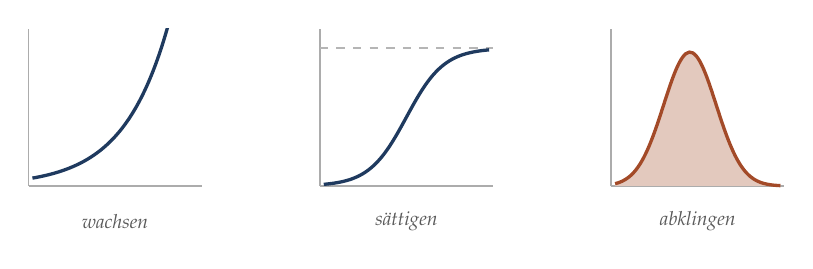
\begin{tikzpicture}[scale=1.0]
% exponentiell
\begin{scope}[xshift=-3.7cm]
\draw[grau!50, line width=0.6pt] (-1.1,-0.85) -- (-1.1,1.15);
\draw[grau!50, line width=0.6pt] (-1.1,-0.85) -- (1.1,-0.85);
\begin{scope}
\clip (-1.1,-0.86) rectangle (1.1,1.15);
\draw[tief, line width=1.2pt, smooth, samples=60, domain=-1.05:1.05]
  plot (\x, {-0.85 + 0.10*exp(1.75*(\x+1.05))});
\end{scope}
\node[font=\scriptsize\itshape, color=grau] at (0,-1.3) {wachsen};
\end{scope}
% logistisch
\begin{scope}
\draw[grau!50, line width=0.6pt] (-1.1,-0.85) -- (-1.1,1.15);
\draw[grau!50, line width=0.6pt] (-1.1,-0.85) -- (1.1,-0.85);
\draw[grau!45, dashed, line width=0.5pt] (-1.1,0.9) -- (1.1,0.9);
\draw[tief, line width=1.2pt, smooth, samples=60, domain=-1.05:1.05]
  plot (\x, {-0.85 + 1.75/(1+exp(-4.2*\x))});
\node[font=\scriptsize\itshape, color=grau] at (0,-1.3) {sättigen};
\end{scope}
% Epidemiekurve
\begin{scope}[xshift=3.7cm]
\draw[grau!50, line width=0.6pt] (-1.1,-0.85) -- (-1.1,1.15);
\draw[grau!50, line width=0.6pt] (-1.1,-0.85) -- (1.1,-0.85);
\fill[akzent!30] plot[smooth, samples=50, domain=-1.05:1.05] (\x,{-0.85+1.7*exp(-4.5*(\x+0.1)*(\x+0.1))}) -- (1.05,-0.85) -- (-1.05,-0.85) -- cycle;
\draw[akzent, line width=1.2pt, smooth, samples=50, domain=-1.05:1.05]
  plot (\x, {-0.85 + 1.7*exp(-4.5*(\x+0.1)*(\x+0.1))});
\node[font=\scriptsize\itshape, color=grau] at (0,-1.3) {abklingen};
\end{scope}
\end{tikzpicture}

\vspace{1.4cm}
{\large\color{grau} Von der Zellteilung bis zum Epidemieverlauf}\\[6pt]
{\color{grau} Jeder Schritt erklärt. Mit vollständig durchgerechneten Übungsaufgaben.}\\[1.9cm]
{\small\color{grau} Stand der Forschung: August 2026}
\end{titlepage}
\thispagestyle{empty}
\vspace*{\fill}
\begin{flushleft}
{\small\color{grau}
\textbf{\color{tief}Mathematik von Grund auf} --- Band 18\\[2pt]
\textit{Wachsen und Vergehen} $\cdot$ Biomathematik\\[14pt]

Herausgeber und Urheber: Jürgen Maier\\[2pt]
Entstanden 2026 in Zusammenarbeit mit Claude (Anthropic); Konzeption, Vorgaben, Prüfung und Herausgeberschaft: Jürgen Maier.\\[14pt]

\textbf{Lizenz}\\[2pt]
Dieses Werk ist lizenziert unter einer Creative-Commons-Lizenz \textbf{Namensnennung -- Weitergabe unter gleichen Bedingungen 4.0 International (CC BY-SA 4.0)}. Sie dürfen das Werk vervielfältigen, verbreiten, bearbeiten und auch kommerziell nutzen, sofern Sie den Urheber nennen und Bearbeitungen unter derselben Lizenz weitergeben.\\[2pt]
Lizenztext: \texttt{https://creativecommons.org/licenses/by-sa/4.0/legalcode.de}\\[14pt]

\textbf{Quellen und Fassungen}\\[2pt]
Quelltexte, Simulationen, Fehlermeldungen und aktuelle Fassungen aller Bände:\\
\texttt{https://github.com/juergenmaier2026/mathematik-von-grund-auf}\\[2pt]
Dauerhaft archiviert bei Zenodo: \texttt{https://doi.org/10.5281/zenodo.23698547}\\[14pt]

\textbf{Zitiervorschlag}\\[2pt]
Maier, J. (2026). \textit{Mathematik von Grund auf, Band 18: Wachsen und Vergehen}. Fassung 1.0.1. \texttt{https://doi.org/10.5281/zenodo.23698547}\\[14pt]

Satz: \LaTeX{} mit Palatino. Fassung 1.0.1, Oktober 2026. 262 Seiten.
}
\end{flushleft}
\vspace*{1.5cm}

\tableofcontents
\mainmatter

\chapter*{Vorwort: Was ein Modell kann}
\addcontentsline{toc}{chapter}{Vorwort}
\markboth{Vorwort}{Vorwort}

Die Biomathematik ist das Gebiet, in dem die Mathematik am sichtbarsten \kursiv{scheitert} --- und gerade deshalb am meisten leistet.

\begin{merksatz}
\boxtitel{Der Ausgangspunkt}
\begin{center}
\begin{minipage}{0.9\textwidth}
Jedes Modell dieses Bandes ist falsch. Kein Bakterium teilt sich exakt nach einer Exponentialfunktion, keine Epidemie verläuft wie eine Gleichung, kein Wirkstoff verteilt sich in drei wohldefinierten Behältern.
\end{minipage}
\end{center}

\begin{center}
\begin{minipage}{0.88\textwidth}
\kursiv{Die Frage ist daher nie, ob ein Modell stimmt --- es stimmt nie. Die Frage lautet: Welche Auskunft gibt es trotzdem, und ab wann führt es in die Irre? Das ist die Leitfrage dieses Bandes, und sie steht in jedem Kapitel als eigener Abschnitt.}
\end{minipage}
\end{center}
\end{merksatz}

\section*{Warum sich das lohnt}

\begin{merksatz}
\boxtitel{Vier Dinge, die ein Modell leistet}
\begin{center}
{\small
\renewcommand{\arraystretch}{1.55}
\begin{tabular}{@{}P{3.0cm}P{5.6cm}@{}}
\toprule
\textbf{Zusammen\-hänge sichtbar machen} & Warum wirkt eine Impfquote von $80\,\%$ anders als eine von $60\,\%$? Die Antwort ist eine Schwelle, und man sieht sie nur in der Gleichung.\\
\textbf{Größen abschätzen} & Wie lange dauert es, bis ein Wirkstoffspiegel sein Gleichgewicht erreicht? Vier Halbwertszeiten --- das folgt aus der Rechnung, nicht aus der Erfahrung.\\
\textbf{Annahmen prüfen} & Ein Modell zwingt dazu, alle Annahmen aufzuschreiben. Widersprüche werden dabei sichtbar.\\
\textbf{Überraschungen erzeugen} & Einige Ergebnisse dieses Bandes widersprechen der Anschauung --- und sind trotzdem richtig.\\
\bottomrule
\end{tabular}}
\end{center}

\begin{center}
\begin{minipage}{0.88\textwidth}
\kursiv{Zur letzten Zeile ein Vorgriff: Eine einfache Gleichung für eine Insektenpopulation --- eine Zeile, drei Zeichen --- erzeugt bei bestimmten Parameterwerten einen Verlauf, der sich nie wiederholt und von keiner Rechnung vorhersagen lässt. Kapitel~3 führt das vor. Es war eine der folgenreichsten Entdeckungen der Mathematik des zwanzigsten Jahrhunderts, und sie stammt aus der Biologie.}
\end{minipage}
\end{center}
\end{merksatz}

\begin{warnung}
\boxtitelr{Der Aufbau jedes Kapitels}
\begin{center}
\renewcommand{\arraystretch}{1.5}
\begin{tabular}{@{}P{2.4cm}P{6.2cm}@{}}
\toprule
\textbf{Die Annahme} & Was genau wird unterstellt? In Worten, vor jeder Formel.\\
\textbf{Die Gleichung} & Aus der Annahme aufgestellt, Schritt für Schritt.\\
\textbf{Die Lösung} & Vollständig hergeleitet, nicht nachgeschlagen.\\
\textbf{Die Deutung} & Was bedeuten die Parameter in der Sache?\\
\textbf{Der Bruchfall} & Wo versagt das Modell, und woran erkennt man es?\\
\bottomrule
\end{tabular}
\end{center}

\begin{center}
\begin{minipage}{0.88\textwidth}
\kursiv{Der letzte Punkt ist derselbe wie in Band 17. Ein Modell, dessen Grenzen man nicht kennt, wendet man blind an --- und in der Biomathematik sind diese Grenzen oft näher, als die Eleganz der Gleichungen vermuten lässt.}
\end{minipage}
\end{center}
\end{warnung}

\section*{Was Sie mitbringen müssen}

\begin{merksatz}
\boxtitel{Die Voraussetzungen}
\begin{center}
{\small
\renewcommand{\arraystretch}{1.5}
\begin{tabular}{@{}P{3.0cm}P{5.6cm}@{}}
\toprule
\textbf{Ableiten} & Was $f'(x)$ bedeutet und wie man Polynome, Exponentialfunktionen und Produkte ableitet. Band 3.\\
\textbf{Integrieren} & Stammfunktionen der Grundfunktionen; Trennung der Veränderlichen wird in Kapitel~1 vorgeführt.\\
\textbf{Exponential und Logarithmus} & Die Rechenregeln. Band 0, Teil~IV.\\
\textbf{Matrizen} & Erst ab Kapitel~6, und dort nur $2\times2$. Band 2.\\
\textbf{Statistik} & Nicht nötig. Wo Daten vorkommen, wird auf Band 17 verwiesen.\\
\bottomrule
\end{tabular}}
\end{center}

\begin{center}
\begin{minipage}{0.88\textwidth}
\kursiv{Band 14 \enquote{Die Gesetze der Veränderung} behandelt Differentialgleichungen allgemein und systematisch. Dieser Band setzt ihn nicht voraus: Jede benötigte Lösungsmethode wird an der Stelle hergeleitet, an der sie gebraucht wird. Wer die Theorie dahinter sehen will, findet sie dort.}
\end{minipage}
\end{center}
\end{merksatz}

\section*{Neustadt und sein Klinikum}

\begin{merksatz}
\boxtitel{Der Leitfall}
Wie in Band 17 läuft ein einziger erfundener Fall durch alle fünfzehn Kapitel.

\begin{center}
\begin{minipage}{0.9\textwidth}
In der Stadt \textbf{Neustadt} mit $100\,000$ Einwohnern breitet sich ein bakterieller Erreger aus. Am Klinikum wird er in Kulturen untersucht, mit einem Antibiotikum behandelt --- und nach einigen Monaten treten erste unempfindliche Stämme auf.
\end{minipage}
\end{center}

\begin{center}
{\small
\renewcommand{\arraystretch}{1.5}
\begin{tabular}{@{}P{1.6cm}P{2.8cm}P{3.6cm}@{}}
\toprule
\textbf{Teil} & \textbf{Thema} & \textbf{Der Leitfall zeigt}\\
\midrule
I & Wachstum & die Kultur im Labor\\
II & Wechselwirkung & zwei Stämme im selben Nährmedium\\
III & Ausbreitung & die Epidemie in Neustadt\\
IV & Der Körper & das Antibiotikum im Patienten\\
V & Krankheit & die Entstehung der Resistenz\\
VI & Stand & was die Forschung heute kann\\
\bottomrule
\end{tabular}}
\end{center}

\begin{center}
\begin{minipage}{0.88\textwidth}
\kursiv{Die Zahlen sind erfunden und so gewählt, dass sie sich von Hand rechnen lassen. Sie sind aber der Größenordnung nach realistisch --- Verdopplungszeiten, Halbwertszeiten und Reproduktionszahlen liegen in Bereichen, die man aus der Literatur kennt.}
\end{minipage}
\end{center}
\end{merksatz}

\section*{Drei Warnungen}

\begin{warnung}
\boxtitelr{Erstens: Parameter sind keine Naturkonstanten}
In jeder Gleichung dieses Bandes stehen Buchstaben wie $r$, $K$, $\beta$. Sie sehen aus wie feste Größen. Sie sind es nicht.

\begin{center}
\begin{minipage}{0.9\textwidth}
Eine Wachstumsrate hängt von Temperatur, Nährstoffen und Stamm ab. Eine Übertragungsrate hängt vom Verhalten der Menschen ab --- und ändert sich, sobald über die Epidemie berichtet wird.
\end{minipage}
\end{center}

\kursiv{Wer einen Parameter aus Daten schätzt, schätzt ihn für die Umstände, unter denen die Daten entstanden.}
\end{warnung}

\begin{warnung}
\boxtitelr{Zweitens: Genauigkeit ist nicht Richtigkeit}
Ein Modell liefert Zahlen mit beliebig vielen Stellen. Das verführt dazu, sie für genau zu halten.

Bei Epidemiemodellen ist der Fehler besonders groß: Kleine Änderungen der Übertragungsrate verändern den Verlauf erheblich, weil sie sich über viele Generationen aufschaukeln. Kapitel~7 rechnet das vor.
\end{warnung}

\begin{warnung}
\boxtitelr{Drittens: Das einfachste Modell ist oft das nützlichste}
Man kann jedes Modell verfeinern --- Altersgruppen, räumliche Verteilung, Verhaltensänderung. Jede Verfeinerung fügt Parameter hinzu, die man nicht kennt.

\begin{center}
\begin{minipage}{0.88\textwidth}
\kursiv{Ein Modell mit drei Gleichungen, dessen Verhalten man versteht, ist einem mit dreißig überlegen, dessen Ergebnis man nur glauben kann. Die Aufgabe der Modellierung ist nicht, die Wirklichkeit nachzubauen --- dafür gibt es die Wirklichkeit.}
\end{minipage}
\end{center}
\end{warnung}

\section*{Der Aufbau}

\begin{merksatz}
\boxtitel{Sechs Teile, fünfzehn Kapitel}
\begin{center}
{\small
\renewcommand{\arraystretch}{1.45}
\begin{tabular}{@{}P{1.0cm}P{3.0cm}P{4.6cm}@{}}
\toprule
\textbf{Teil} & \textbf{Thema} & \textbf{Die Leitfrage}\\
\midrule
I & Wachstum (1--3) & Wie viel wird daraus?\\
II & Wechselwirkung (4--6) & Was geschieht, wenn zwei sich beeinflussen?\\
III & Ausbreitung (7--9) & Wann bricht eine Epidemie aus?\\
IV & Der Körper (10--12) & Wie verteilt und wirkt ein Stoff?\\
V & Krankheit (13--14) & Wie wachsen Tumoren, wie entsteht Resistenz?\\
VI & Stand (15) & Was können Modelle heute?\\
\bottomrule
\end{tabular}}
\end{center}
\end{merksatz}

\vspace{10pt}
\begin{flushright}
\itshape\color{grau}
Alle Modelle sind falsch.\\
Einige sind brauchbar.\\[8pt]
\normalfont\color{grau}\upshape --- George Box, 1976
\end{flushright}

\part{Wachstum}

\chapter{Exponentielles Wachstum}

\section{Die Annahme}

\begin{merksatz}
\boxtitel{Der Leitfall beginnt im Labor}
Am Klinikum Neustadt wird der Erreger in einer Nährlösung angezüchtet. Zu Beginn enthält ein Milliliter etwa $10^4$ Bakterien. Unter günstigen Bedingungen teilt sich jede Zelle etwa alle dreißig Minuten.

\textbf{Die Frage:} Wie viele sind es nach acht Stunden?
\end{merksatz}

\begin{merksatz}
\boxtitel{Die Annahme in Worten --- vor jeder Formel}
\begin{center}
\begin{minipage}{0.9\textwidth}
\textbf{Jede Zelle teilt sich unabhängig von den anderen mit derselben Rate. Nichts hindert sie daran.}
\end{minipage}
\end{center}

Daraus folgt: Die Zahl der Neuzugänge je Zeiteinheit ist \kursiv{proportional} zur vorhandenen Zahl. Doppelt so viele Zellen erzeugen doppelt so viele Neue.

\begin{center}
\begin{minipage}{0.88\textwidth}
\kursiv{Das ist die gesamte Annahme. Alles Weitere in diesem Kapitel folgt aus ihr --- und alle Schwierigkeiten, die in Kapitel~2 auftreten, stammen daher, dass sie auf Dauer nicht zutrifft.}
\end{minipage}
\end{center}
\end{merksatz}

\begin{definition}
\boxtitelm{Definition 1.1 --- die Wachstumsgleichung}
Sei $N(t)$ die Anzahl zur Zeit~$t$. Die Annahme lautet in Zeichen
\[ \frac{\dd N}{\dd t} \;=\; r\,N \]
mit der \Begriff{Wachstums\-rate} $r > 0$.
\end{definition}

\begin{merksatz}
\boxtitel{Wie man die Gleichung liest}
\begin{center}
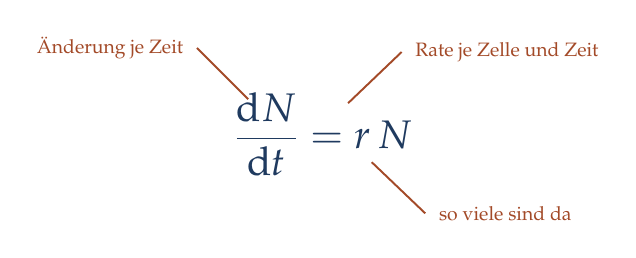
\begin{tikzpicture}[scale=1.0]
\node[font=\Large, color=tief] at (0,0) {$\displaystyle \frac{\dd N}{\dd t} = r\,N$};
\draw[akzent, line width=0.7pt] (-0.95,0.45) -- (-1.6,1.1);
\node[font=\scriptsize, color=akzent, anchor=east] at (-1.65,1.1) {Änderung je Zeit};
\draw[akzent, line width=0.7pt] (0.62,-0.35) -- (1.3,-1.0);
\node[font=\scriptsize, color=akzent, anchor=west] at (1.35,-1.0) {so viele sind da};
\draw[akzent, line width=0.7pt] (0.32,0.4) -- (1.0,1.05);
\node[font=\scriptsize, color=akzent, anchor=west] at (1.05,1.05) {Rate je Zelle und Zeit};
\end{tikzpicture}
\end{center}

\schritt{Die Einheit von $r$}
Links steht \enquote{Zellen je Stunde}, rechts \enquote{$r$ mal Zellen}. Damit beides übereinstimmt, muss $r$ die Einheit \enquote{je Stunde} tragen --- also $\mathrm{h}^{-1}$.

\begin{center}
\begin{minipage}{0.88\textwidth}
\kursiv{Diese Einheitenprüfung ist keine Formsache. Sie ist die schnellste Art, einen Fehler in einem Modell zu finden: Wenn die Einheiten nicht zusammenpassen, stimmt die Gleichung nicht --- gleichgültig wie plausibel sie aussieht.}
\end{minipage}
\end{center}

\schritt{Was $r$ bedeutet}
\[ r = \frac{1}{N}\cdot\frac{\dd N}{\dd t} \]
Das ist die \kursiv{relative} Zuwachsrate: der Zuwachs je vorhandener Zelle und Zeiteinheit. Bei $r = 0{,}5\,\mathrm{h}^{-1}$ wächst die Kultur in jeder Stunde um etwa die Hälfte ihres Bestands.
\end{merksatz}

\section{Die Lösung}

\begin{merksatz}
\boxtitel{Satz 1.2 --- Trennung der Veränderlichen}
Die Lösung von $\dfrac{\dd N}{\dd t} = rN$ mit $N(0) = N_0 > 0$ lautet
\[ N(t) = N_0\,e^{rt} . \]
\end{merksatz}

\begin{merksatz}
\boxtitel{Beweis --- in fünf Schritten}
\schritt{Schritt 1 --- Sortieren}
Wir bringen alles mit $N$ nach links, alles mit $t$ nach rechts. Da $N > 0$ ist, darf man durch $N$ teilen:
\[ \frac{1}{N}\,\dd N = r\,\dd t . \]

\begin{center}
\begin{minipage}{0.88\textwidth}
\kursiv{Diese Schreibweise --- mit $\dd N$ und $\dd t$ als getrennten Größen --- ist streng genommen eine Abkürzung. Sie lässt sich rechtfertigen, und Band 14 tut das. Für unsere Zwecke genügt es zu wissen, dass das Ergebnis korrekt ist und sich durch Einsetzen prüfen lässt --- was wir in Schritt 5 tun.}
\end{minipage}
\end{center}

\schritt{Schritt 2 --- Beide Seiten integrieren}
\[ \int \frac{1}{N}\,\dd N = \int r\,\dd t \]
\[ \ln N = r\,t + C \]
Die Stammfunktion von $1/N$ ist $\ln N$ (für $N>0$), die von der Konstanten $r$ ist $rt$. Die beiden Integrationskonstanten fasst man zu einer zusammen.

\schritt{Schritt 3 --- Nach $N$ auflösen}
\[ N = e^{rt + C} = e^{C}\cdot e^{rt} \]
Die Zahl $e^C$ ist positiv, aber unbekannt. Wir nennen sie $A$:
\[ N(t) = A\,e^{rt} . \]

\schritt{Schritt 4 --- Die Konstante bestimmen}
Zur Zeit $t=0$ gilt
\[ N(0) = A\,e^{0} = A \cdot 1 = A . \]
Also ist $A = N_0$, und
\[ N(t) = N_0\,e^{rt} . \]

\schritt{Schritt 5 --- Die Probe}
Wir setzen die gefundene Lösung in die ursprüngliche Gleichung ein.

\kursiv{Linke Seite:}
\[ \frac{\dd}{\dd t}\Bigl(N_0e^{rt}\Bigr) = N_0 \cdot r\,e^{rt} = r\,N_0e^{rt} \]
nach der Kettenregel.

\kursiv{Rechte Seite:}
\[ r\,N(t) = r\,N_0e^{rt} \]

Beide stimmen überein. Und $N(0) = N_0$. \checkmark\ $\blacksquare$

\begin{center}
\begin{minipage}{0.88\textwidth}
\kursiv{Schritt 5 ist nicht bloße Sorgfalt. Die Trennung der Veränderlichen ist ein Verfahren, das \kursiv{Kandidaten} liefert; erst die Probe macht daraus eine Lösung. In diesem Band wird jede Lösung geprüft.}
\end{minipage}
\end{center}
\end{merksatz}

\section{Verdopplungszeit}

\begin{merksatz}
\boxtitel{Satz 1.3}
Die Zeit, in der sich der Bestand verdoppelt, beträgt
\[ T_2 = \frac{\ln 2}{r} \]
und hängt \kursiv{nicht} vom Ausgangswert ab.

\schritt{Beweis}
Gesucht ist $T_2$ mit $N(t+T_2) = 2\,N(t)$:
\begin{align*}
N_0e^{r(t+T_2)} &= 2\,N_0e^{rt}\\
e^{rt}\cdot e^{rT_2} &= 2\,e^{rt}\\
e^{rT_2} &= 2 && \text{(durch } e^{rt} \neq 0 \text{ geteilt)}\\
rT_2 &= \ln 2\\
T_2 &= \frac{\ln 2}{r} . \qquad \blacksquare
\end{align*}

\schritt{Die bemerkenswerte Eigenschaft}
In der Rechnung fiel $e^{rt}$ vollständig heraus --- und mit ihm $N_0$ und $t$.

\begin{center}
\begin{minipage}{0.9\textwidth}
\textbf{Von $10$ auf $20$ dauert genauso lange wie von $10^{12}$ auf $2\cdot10^{12}$.} Diese Eigenschaft kennzeichnet das exponentielle Wachstum und kein anderes.
\end{minipage}
\end{center}
\end{merksatz}

\begin{merksatz}
\boxtitel{Die Kultur am Klinikum}
\schritt{Schritt 1 --- Die Rate bestimmen}
Gegeben ist $T_2 = 30\ \text{min} = 0{,}5\ \text{h}$. Aus Satz 1.3:
\[ r = \frac{\ln 2}{T_2} = \frac{0{,}6931}{0{,}5} = 1{,}386\ \mathrm{h}^{-1} . \]

\schritt{Schritt 2 --- Nach acht Stunden}
\[ N(8) = 10^4 \cdot e^{1{,}386 \cdot 8} = 10^4 \cdot e^{11{,}09} \]
\[ e^{11{,}09} = 65\,536 \]
\[ N(8) = 10^4 \cdot 65\,536 = 6{,}55 \cdot 10^{8} \ \text{je Milliliter} . \]

\schritt{Schritt 3 --- Die Kontrolle ohne $e$}
In acht Stunden liegen $8/0{,}5 = 16$ Verdopplungen. Also
\[ N(8) = 10^4 \cdot 2^{16} = 10^4 \cdot 65\,536 . \quad \checkmark \]

\begin{center}
\begin{minipage}{0.88\textwidth}
\kursiv{Die zweite Rechnung ist die anschaulichere und sollte immer mitlaufen: Verdopplungen zählen ist einfacher als Exponenten ausrechnen und macht Größenordnungsfehler sofort sichtbar.}
\end{minipage}
\end{center}

\schritt{Schritt 4 --- Der Bezug zur Praxis}
Eine Keimzahl von $10^8$ bis $10^9$ je Milliliter ist die Größenordnung, bei der eine Bakterienkultur sichtbar trüb wird. Nach acht Stunden ist die Nährlösung also erkennbar bewachsen --- was mit der Laborerfahrung übereinstimmt.
\end{merksatz}

\section{Der Bruchfall}

Jetzt der wichtigste Abschnitt des Kapitels.

\begin{warnung}
\boxtitelr{Nichts wächst lange exponentiell}
Rechnen wir weiter. Nach $48$ Stunden lägen $96$ Verdopplungen vor:
\[ N(48) = 10^4 \cdot 2^{96} = 10^4 \cdot 7{,}92\cdot10^{28} = 7{,}9\cdot10^{32} \ \text{je Milliliter} . \]

\schritt{Was das bedeutet}
Eine Bakterienzelle wiegt etwa $10^{-12}$ Gramm. Ein Milliliter Kultur wöge dann
\[ 7{,}9\cdot10^{32} \cdot 10^{-12}\ \text{g} = 7{,}9\cdot10^{20}\ \text{g} = 7{,}9\cdot10^{17}\ \text{kg} . \]

\schritt{Wann die Erdmasse erreicht wäre}
Die Erde wiegt $5{,}97\cdot10^{24}$ kg, also $5{,}97\cdot10^{27}$ g --- das sind $5{,}97\cdot10^{39}$ Bakterien.

Von $10^4$ aus braucht man den Faktor $5{,}97\cdot10^{35}$, also
\[ \log_2\bigl(5{,}97\cdot10^{35}\bigr) = \frac{35{,}78}{0{,}301} = 118{,}9 \ \text{Verdopplungen} , \]
das sind $118{,}9 \cdot 0{,}5 = 59{,}4$ Stunden.

\begin{center}
\begin{minipage}{0.9\textwidth}
\textbf{Nach zweieinhalb Tagen wöge ein Milliliter Kultur so viel wie die Erde.}
\end{minipage}
\end{center}

\begin{center}
\begin{minipage}{0.88\textwidth}
\kursiv{Das ist kein Rechenfehler, sondern die korrekte Folgerung aus der Annahme. Es zeigt, dass die Annahme falsch sein muss --- und zwar lange vorher. Ein Modell an seine Grenze zu treiben, ist die beste Art, seine Grenze zu finden.}
\end{minipage}
\end{center}
\end{warnung}

\begin{merksatz}
\boxtitel{Woran die Annahme scheitert}
\begin{center}
{\small
\renewcommand{\arraystretch}{1.5}
\begin{tabular}{@{}P{3.0cm}P{5.6cm}@{}}
\toprule
\textbf{Nährstoffe} & Sie werden knapp. Die Teilungsrate sinkt.\\
\textbf{Abfallstoffe} & Sie reichern sich an und hemmen das Wachstum.\\
\textbf{Platz} & Das Volumen ist endlich.\\
\textbf{Wechsel\-wirkung} & \kursiv{Jede} Zelle teilt sich unabhängig --- das setzt voraus, dass sie einander nicht bemerken.\\
\bottomrule
\end{tabular}}
\end{center}

\schritt{Die typische Wachstumskurve im Labor}
\begin{center}
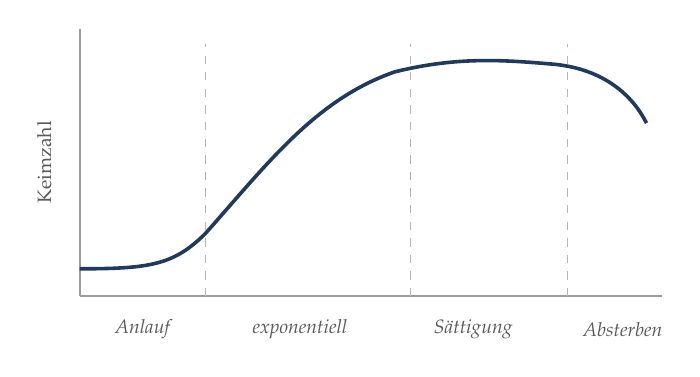
\begin{tikzpicture}[scale=1.0]
\draw[grau!60, line width=0.7pt] (0,0) -- (7.4,0);
\draw[grau!60, line width=0.7pt] (0,0) -- (0,3.4);
\draw[tief, line width=1.3pt]
  (0,0.35) .. controls (0.9,0.35) and (1.2,0.4) .. (1.6,0.8)
  .. controls (2.4,1.7) and (3.0,2.5) .. (4.0,2.85)
  .. controls (4.8,3.05) and (5.4,3.0) .. (6.0,2.95)
  .. controls (6.6,2.9) and (7.0,2.6) .. (7.2,2.2);
\foreach \x/\lab in {0.8/{Anlauf}, 2.8/{exponentiell}, 5.0/{Sättigung}, 6.9/{Absterben}}
  \node[font=\scriptsize\itshape, color=grau] at (\x,-0.42) {\lab};
\draw[grau!45, dashed] (1.6,0) -- (1.6,3.2);
\draw[grau!45, dashed] (4.2,0) -- (4.2,3.2);
\draw[grau!45, dashed] (6.2,0) -- (6.2,3.2);
\node[font=\scriptsize, color=grau, rotate=90] at (-0.45,1.7) {Keimzahl};
\end{tikzpicture}
\end{center}

\begin{center}
\begin{minipage}{0.9\textwidth}
\textbf{Das exponentielle Modell beschreibt genau den zweiten Abschnitt --- und nur ihn.} Er dauert im Labor typischerweise einige Stunden.
\end{minipage}
\end{center}

\begin{center}
\begin{minipage}{0.88\textwidth}
\kursiv{Das ist die ehrliche Beschreibung: Das Modell ist nicht falsch, sondern \kursiv{lokal} gültig. Kapitel~2 erweitert es so, dass es auch den dritten Abschnitt erfasst.}
\end{minipage}
\end{center}
\end{merksatz}

\section{Die halblogarithmische Darstellung}

\begin{merksatz}
\boxtitel{Wie man exponentielles Wachstum erkennt}
Logarithmiert man die Lösung, so wird sie linear:
\[ \ln N(t) = \ln\bigl(N_0e^{rt}\bigr) = \ln N_0 + rt . \]

\begin{center}
\begin{minipage}{0.9\textwidth}
\textbf{Trägt man $\ln N$ gegen $t$ auf, so liegt exponentielles Wachstum auf einer Geraden --- mit der Steigung $r$ und dem Achsenabschnitt $\ln N_0$.}
\end{minipage}
\end{center}

\begin{center}
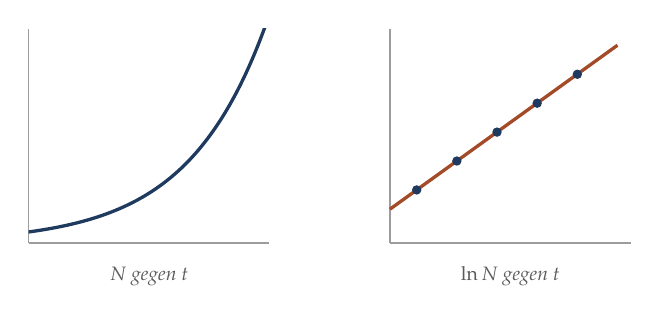
\begin{tikzpicture}[scale=0.85]
\begin{scope}
\draw[grau!60, line width=0.6pt] (0,0) -- (3.6,0);
\draw[grau!60, line width=0.6pt] (0,0) -- (0,3.2);
\begin{scope}
\clip (0,0) rectangle (3.6,3.2);
\draw[tief, line width=1.2pt, smooth, samples=50, domain=0:3.6]
  plot (\x, {0.16*exp(0.85*\x)});
\end{scope}
\node[font=\scriptsize\itshape, color=grau] at (1.8,-0.5) {$N$ gegen $t$};
\end{scope}
\begin{scope}[xshift=5.4cm]
\draw[grau!60, line width=0.6pt] (0,0) -- (3.6,0);
\draw[grau!60, line width=0.6pt] (0,0) -- (0,3.2);
\draw[akzent, line width=1.2pt] (0,0.5) -- (3.4,2.95);
\foreach \x in {0.4,1.0,1.6,2.2,2.8}
  \fill[tief] (\x,{0.5+0.72*\x}) circle (2.0pt);
\node[font=\scriptsize\itshape, color=grau] at (1.8,-0.5) {$\ln N$ gegen $t$};
\end{scope}
\end{tikzpicture}
\end{center}

\schritt{Wozu das gut ist}
\begin{center}
\renewcommand{\arraystretch}{1.5}
\begin{tabular}{@{}P{2.4cm}P{6.2cm}@{}}
\toprule
\textbf{Prüfen} & Krümmt sich die Linie, ist das Wachstum nicht exponentiell --- das sieht man in der gewöhnlichen Darstellung nicht.\\
\textbf{Schätzen} & Die Steigung liefert $r$ unmittelbar. Kapitel~10 in Band 17 zeigt, wie man sie bestimmt.\\
\textbf{Darstellen} & Über viele Größenordnungen bleibt alles sichtbar.\\
\bottomrule
\end{tabular}
\end{center}

\begin{center}
\begin{minipage}{0.88\textwidth}
\kursiv{Die erste Zeile ist der eigentliche Nutzen. In der gewöhnlichen Darstellung sieht jedes rasche Wachstum gleich aus --- eine steile Kurve. Erst die logarithmische Achse trennt exponentielles von überexponentiellem und von gesättigtem Wachstum.}
\end{minipage}
\end{center}
\end{merksatz}

\section{Zerfall: dieselbe Gleichung mit anderem Vorzeichen}

\begin{merksatz}
\boxtitel{Wenn $r$ negativ ist}
Setzt man $r = -k$ mit $k > 0$, so lautet die Gleichung
\[ \frac{\dd N}{\dd t} = -k\,N \qquad\text{mit der Lösung}\qquad N(t) = N_0e^{-kt} . \]

\schritt{Die Annahme in Worten}
\begin{center}
\begin{minipage}{0.9\textwidth}
\textbf{Jedes vorhandene Teilchen verschwindet unabhängig von den anderen mit derselben Wahrscheinlichkeit je Zeiteinheit.}
\end{minipage}
\end{center}

\schritt{Wo das zutrifft}
\begin{center}
{\small
\renewcommand{\arraystretch}{1.5}
\begin{tabular}{@{}P{2.6cm}P{6.0cm}@{}}
\toprule
\textbf{Radioaktiver Zerfall} & Trifft exakt zu --- ein Atomkern hat kein Gedächtnis.\\
\textbf{Arzneimittel} & Trifft näherungsweise zu, solange die abbauenden Enzyme nicht gesättigt sind. Kapitel~10.\\
\textbf{Absterben} & Trifft zu, wenn alle Zellen gleich gefährdet sind.\\
\bottomrule
\end{tabular}}
\end{center}
\end{merksatz}

\begin{merksatz}
\boxtitel{Halbwertszeit}
Dieselbe Rechnung wie in Satz 1.3, mit $\frac12$ statt $2$:
\[ e^{-kT_{1/2}} = \tfrac12 \quad\Longrightarrow\quad -kT_{1/2} = \ln\tfrac12 = -\ln 2 \]
\[ T_{1/2} = \frac{\ln 2}{k} . \]

\schritt{Die Merktabelle}
\begin{center}
\renewcommand{\arraystretch}{1.48}
\begin{tabular}{@{}P{2.6cm}P{2.4cm}P{2.6cm}@{}}
\toprule
\textbf{Nach} & \textbf{Anteil übrig} & \\
\midrule
$1\,T_{1/2}$ & $50{,}0\,\%$ & \\
$2\,T_{1/2}$ & $25{,}0\,\%$ & \\
$3\,T_{1/2}$ & $12{,}5\,\%$ & \\
$4\,T_{1/2}$ & $6{,}25\,\%$ & \textcolor{gruen}{Faustregel}\\
$5\,T_{1/2}$ & $3{,}13\,\%$ & \\
$7\,T_{1/2}$ & $0{,}78\,\%$ & praktisch weg\\
\bottomrule
\end{tabular}
\end{center}

\begin{center}
\begin{minipage}{0.88\textwidth}
\kursiv{Die Zeile mit vier Halbwertszeiten ist die klinisch wichtigste: Nach dieser Zeit sind rund $94\,\%$ eines Wirkstoffs eliminiert. Dieselbe Zahl kehrt in Kapitel~10 in umgekehrter Richtung wieder --- als Zeit bis zum Erreichen des Gleichgewichtsspiegels.}
\end{minipage}
\end{center}
\end{merksatz}

\section{Übungsaufgaben}

\begin{aufgabe}
\boxtitel{Aufgabe 1.1 --- Rate aus zwei Messwerten}
Eine Kultur enthält zur Zeit $t=0$ genau $2{,}0\cdot10^5$ Zellen je Milliliter, nach $3$ Stunden $1{,}8\cdot10^6$. Bestimmen Sie $r$, die Verdopplungszeit und den Bestand nach $7$ Stunden.

\loesung
\schritt{Schritt 1 --- Die Gleichung aufstellen}
\[ N(3) = N_0e^{3r} \quad\Longrightarrow\quad 1{,}8\cdot10^6 = 2{,}0\cdot10^5 \cdot e^{3r} \]

\schritt{Schritt 2 --- Nach $r$ auflösen}
\[ e^{3r} = \frac{1{,}8\cdot10^6}{2{,}0\cdot10^5} = 9{,}0 \]
\[ 3r = \ln 9{,}0 = 2{,}1972 \]
\[ r = \frac{2{,}1972}{3} = 0{,}7324\ \mathrm{h}^{-1} \]

\schritt{Schritt 3 --- Verdopplungszeit}
\[ T_2 = \frac{\ln 2}{r} = \frac{0{,}6931}{0{,}7324} = 0{,}946\ \text{h} = 56{,}8\ \text{min} \]

\schritt{Schritt 4 --- Die Kontrolle über Verdopplungen}
In drei Stunden hat sich der Bestand verneunfacht. Neun liegt zwischen $8 = 2^3$ und $16 = 2^4$, genauer bei
\[ \log_2 9 = \frac{\ln 9}{\ln 2} = \frac{2{,}1972}{0{,}6931} = 3{,}17 \ \text{Verdopplungen} . \]
\[ T_2 = \frac{3\ \text{h}}{3{,}17} = 0{,}946\ \text{h} . \quad \checkmark \]

\schritt{Schritt 5 --- Der Bestand nach sieben Stunden}
\[ N(7) = 2{,}0\cdot10^5 \cdot e^{0{,}7324 \cdot 7} = 2{,}0\cdot10^5 \cdot e^{5{,}127} \]
\[ e^{5{,}127} = 168{,}5 \]
\[ N(7) = 3{,}37\cdot10^{7} \ \text{je Milliliter} \]

\schritt{Schritt 6 --- Die Kontrolle}
Sieben Stunden entsprechen $7/0{,}946 = 7{,}40$ Verdopplungen:
\[ 2^{7{,}40} = 168{,}9 \quad\Longrightarrow\quad 2{,}0\cdot10^5 \cdot 168{,}9 = 3{,}38\cdot10^7 . \quad \checkmark \]

\schritt{Ein Vorbehalt}
Die Rechnung setzt voraus, dass das Wachstum über die ganzen sieben Stunden exponentiell bleibt. Bei $3{,}4\cdot10^7$ je Milliliter ist das plausibel --- die Sättigung setzt meist erst bei $10^8$ bis $10^9$ ein.

\begin{center}
\begin{minipage}{0.86\textwidth}
\kursiv{Hätte man nach $24$ Stunden gefragt, so ergäbe die Formel $8{,}8\cdot10^{12}$ --- weit jenseits des Möglichen. Die Antwort wäre rechnerisch richtig und sachlich unbrauchbar. Jede Hochrechnung mit einem Wachstumsmodell braucht die Frage, ob das Modell dort noch gilt.}
\end{minipage}
\end{center}
\end{aufgabe}

\begin{aufgabe}
\boxtitel{Aufgabe 1.2 --- Wirkstoffelimination}
Ein Antibiotikum hat eine Halbwertszeit von $4$ Stunden. Nach einer Einmalgabe beträgt die Spitzenkonzentration $32\ \mathrm{mg/l}$. Die wirksame Mindestkonzentration liegt bei $2\ \mathrm{mg/l}$.
\begin{center}
{\small
\renewcommand{\arraystretch}{1.35}
\begin{tabular}{@{}P{4.2cm}P{4.2cm}@{}}
\toprule
(a) Eliminationskonstante $k$ & (c) Wie lange über $2\ \mathrm{mg/l}$?\\
(b) Konzentration nach $6$ h & (d) Welches Dosierungsintervall?\\
\bottomrule
\end{tabular}}
\end{center}

\loesung
\schritt{(a) --- Die Konstante}
\[ k = \frac{\ln 2}{T_{1/2}} = \frac{0{,}6931}{4} = 0{,}1733\ \mathrm{h}^{-1} \]

\schritt{(b) --- Nach sechs Stunden}
\[ c(6) = 32 \cdot e^{-0{,}1733 \cdot 6} = 32 \cdot e^{-1{,}0397} = 32 \cdot 0{,}3536 = 11{,}3\ \mathrm{mg/l} \]

\kursiv{Kontrolle:} Sechs Stunden sind $1{,}5$ Halbwertszeiten. Also
\[ 32 \cdot \left(\tfrac12\right)^{1{,}5} = 32 \cdot 0{,}3536 = 11{,}3 . \quad \checkmark \]

\schritt{(c) --- Die Zeit bis zur Mindestkonzentration}
\[ 2 = 32\,e^{-kt} \quad\Longrightarrow\quad e^{-kt} = \frac{2}{32} = \frac{1}{16} \]
\[ -kt = \ln\tfrac{1}{16} = -\ln 16 = -2{,}7726 \]
\[ t = \frac{2{,}7726}{0{,}1733} = 16{,}0\ \text{h} \]

\kursiv{Die Kontrolle in Halbwertszeiten:} Von $32$ auf $2$ ist der Faktor $16 = 2^4$, also genau vier Halbwertszeiten:
\[ 4 \cdot 4\ \text{h} = 16\ \text{h} . \quad \checkmark \]

\schritt{(d) --- Das Dosierungsintervall}
Soll die Konzentration nie unter $2\ \mathrm{mg/l}$ fallen, so darf das Intervall höchstens $16$ Stunden betragen. In der Praxis wählte man $12$ Stunden --- zweimal täglich --- mit Sicherheitsabstand.

\schritt{Ein Vorbehalt zu dieser Rechnung}
Die Rechnung betrachtet eine \kursiv{Einmalgabe}. Bei wiederholter Gabe reichert sich der Wirkstoff an, und die Spitzenkonzentration steigt von Gabe zu Gabe, bis sich ein Gleichgewicht einstellt.

\begin{center}
\begin{minipage}{0.86\textwidth}
\kursiv{Kapitel~10 rechnet das vollständig durch. Das Ergebnis vorweg: Das Gleichgewicht ist nach etwa vier Halbwertszeiten erreicht --- hier also nach $16$ Stunden, unabhängig von der Dosis. Es ist dieselbe Zahl wie in Teil (c), und das ist kein Zufall.}
\end{minipage}
\end{center}
\end{aufgabe}

\begin{aufgabe}
\boxtitel{Aufgabe 1.3 --- Zwei Stämme im Vergleich}
Im Labor wachsen nebeneinander ein empfindlicher Stamm ($T_2 = 30$ min) und ein unempfindlicher ($T_2 = 36$ min). Zu Beginn macht der unempfindliche einen Anteil von $0{,}1\,\%$ aus. Wie entwickelt sich sein Anteil --- ohne Antibiotikum?

\loesung
\schritt{Schritt 1 --- Die beiden Raten}
\[ r_E = \frac{\ln 2}{0{,}5} = 1{,}3863\ \mathrm{h}^{-1}, \qquad r_U = \frac{\ln 2}{0{,}6} = 1{,}1552\ \mathrm{h}^{-1} \]

\schritt{Schritt 2 --- Die Ausgangszahlen}
Sei die Gesamtzahl zu Beginn $N_{\text{ges}} = 10^6$. Dann
\[ E_0 = 0{,}999 \cdot 10^6 = 999\,000, \qquad U_0 = 0{,}001 \cdot 10^6 = 1000 . \]

\schritt{Schritt 3 --- Der Anteil als Funktion der Zeit}
\[ \text{Anteil}(t) = \frac{U_0e^{r_Ut}}{U_0e^{r_Ut} + E_0e^{r_Et}} \]

Wir teilen Zähler und Nenner durch $U_0e^{r_Ut}$:
\[ \text{Anteil}(t) = \frac{1}{1 + \dfrac{E_0}{U_0}\,e^{(r_E-r_U)t}} \]

\schritt{Schritt 4 --- Die maßgebliche Größe}
\[ r_E - r_U = 1{,}3863 - 1{,}1552 = 0{,}2311\ \mathrm{h}^{-1} \]
\[ \frac{E_0}{U_0} = \frac{999\,000}{1000} = 999 \]

\[ \text{Anteil}(t) = \frac{1}{1 + 999\,e^{0{,}2311\,t}} \]

\schritt{Schritt 5 --- Die Werte}
\begin{center}
\renewcommand{\arraystretch}{1.45}
\begin{tabular}{@{}P{1.8cm}P{2.6cm}P{2.6cm}@{}}
\toprule
$t$ (h) & $999\,e^{0{,}2311t}$ & \textbf{Anteil}\\
\midrule
$0$ & $999$ & $0{,}100\,\%$\\
$6$ & $3995$ & $0{,}025\,\%$\\
$12$ & $15\,977$ & $0{,}006\,\%$\\
$24$ & $255\,500$ & $0{,}0004\,\%$\\
\bottomrule
\end{tabular}
\end{center}

\schritt{Schritt 6 --- Die Deutung}
\begin{center}
\begin{minipage}{0.9\textwidth}
\textbf{Der unempfindliche Stamm wird verdrängt.} Sein Anteil viertelt sich etwa alle sechs Stunden.
\end{minipage}
\end{center}

Der Grund steht in Schritt 4: Weil $r_E > r_U$, wächst der Nenner, und der Anteil fällt. Die Unempfindlichkeit kostet Wachstumsgeschwindigkeit --- man nennt das die \Begriff{Fitnesskosten} der Resistenz.

\schritt{Schritt 7 --- Was ein Antibiotikum ändert}
Unter Antibiotikum wird $r_E$ negativ --- der empfindliche Stamm stirbt --- während $r_U$ positiv bleibt. Dann kehrt sich die Rechnung um, und zwar mit derselben Formel: Aus $r_E - r_U > 0$ wird $r_E - r_U < 0$, und der Anteil wächst statt zu fallen.

\begin{center}
\begin{minipage}{0.86\textwidth}
\kursiv{In dieser einen Vorzeichenänderung steckt die gesamte Resistenzproblematik. Kapitel~14 führt sie vollständig aus --- einschließlich der Frage, warum Behandlungspausen die Lage manchmal verbessern und manchmal verschlimmern.}
\end{minipage}
\end{center}
\end{aufgabe}

\begin{geschichte}
\boxtitelg{Ein Pfarrer, ein Pamphlet und ein Streit, der nie aufhörte}
\Person{Thomas Robert Malthus} (1766--1834), anglikanischer Geistlicher und Ökonom, veröffentlichte 1798 anonym eine Schrift über das Bevölkerungsgesetz. Ihr Kern ist die Gegenüberstellung zweier Wachstumsarten:

\begin{center}
\renewcommand{\arraystretch}{1.5}
\begin{tabular}{@{}P{3.0cm}P{5.6cm}@{}}
\toprule
\textbf{Bevölkerung} & wächst \kursiv{geometrisch} --- $1, 2, 4, 8, 16$\\
\textbf{Nahrungs\-mittel} & wachsen \kursiv{arithmetisch} --- $1, 2, 3, 4, 5$\\
\bottomrule
\end{tabular}
\end{center}

Daraus folgerte Malthus, dass die Bevölkerung notwendig an eine Grenze stoße, und zwar durch Hunger, Krankheit oder Krieg.

\begin{center}
\begin{minipage}{0.9\textwidth}
\kursiv{Die erste Behauptung ist mathematisch die Gleichung dieses Kapitels. Die zweite war schon damals nicht begründet und erwies sich als falsch --- die Nahrungsmittelerzeugung wuchs ihrerseits weitgehend exponentiell. Malthus' Vorhersage traf nicht ein; sein mathematischer Kern blieb.}
\end{minipage}
\end{center}

\schritt{Die Wirkung}
Malthus beeinflusste \Person{Charles Darwin} unmittelbar. Darwin schrieb, die Lektüre habe ihm den entscheidenden Gedanken geliefert: Wenn mehr Nachkommen entstehen, als überleben können, muss eine Auslese stattfinden.

\begin{center}
\begin{minipage}{0.9\textwidth}
\kursiv{Das ist die Verbindung, die diesen Band trägt. Exponentielles Wachstum in einer begrenzten Welt \kursiv{erzwingt} Auslese --- und damit alles, was in Teil~II über Konkurrenz und in Teil~V über Resistenz steht. Die Mathematik des ersten Kapitels ist zugleich die Grundlage der Evolutionstheorie.}
\end{minipage}
\end{center}

\Person{Pierre-François Verhulst} nahm Malthus' Gleichung 1838 auf und ergänzte sie um den Sättigungsterm. Davon handelt das nächste Kapitel.
\end{geschichte}

\begin{forschung}
\boxtitelp{Wo exponentielles Wachstum heute gerechnet wird}
\begin{center}
{\small
\renewcommand{\arraystretch}{1.45}
\begin{tabular}{@{}P{3.0cm}P{5.2cm}@{}}
\toprule
\textbf{Frühphase einer Epidemie} & Solange fast alle empfänglich sind, wächst die Fallzahl exponentiell. Die Wachstumsrate ist die zentrale Beobachtungsgröße --- Kapitel~7.\\
\textbf{Tumorzellzahl} & In der frühesten Phase; später deutlich langsamer, Kapitel~13.\\
\textbf{Virus\-vermehrung} & In den ersten Tagen einer Infektion, über mehrere Größenordnungen.\\
\bottomrule
\end{tabular}}
\end{center}

\schritt{Die Verdopplungszeit als Berichtsgröße}
In der Epidemiologie hat sich die Verdopplungszeit gegenüber der Wachstumsrate durchgesetzt --- sie ist anschaulicher und lässt sich schneller einordnen.

\begin{center}
\begin{minipage}{0.88\textwidth}
\kursiv{Beide Angaben sind gleichwertig; man rechnet mit Satz 1.3 ineinander um. Eine Verdopplungszeit von drei Tagen entspricht $r = 0{,}231$ je Tag; eine von einer Woche entspricht $r = 0{,}099$.}
\end{minipage}
\end{center}

\schritt{Die Schwierigkeit beim Schätzen}
Aus Meldedaten die Wachstumsrate zu bestimmen, ist heikler, als es aussieht: Meldeverzüge, Wochenendmuster und wechselnde Testhäufigkeit verzerren die Kurve. Verfahren zur Rückrechnung auf den Erkrankungszeitpunkt sind ein eigenes Forschungsfeld.

\begin{center}
\begin{minipage}{0.88\textwidth}
\kursiv{Das ist die Verbindung zu Band 17: Die Modellrechnung ist der leichtere Teil. Der schwierige ist die Frage, was die Daten eigentlich messen --- und dafür braucht man die Kapitel über Erhebung und Verzerrung.}
\end{minipage}
\end{center}
\end{forschung}

\begin{merksatz}
\boxtitel{Was Sie jetzt können}
\begin{center}
\renewcommand{\arraystretch}{1.5}
\begin{tabular}{@{}P{3.2cm}P{5.4cm}@{}}
\toprule
\textbf{Definition 1.1} & $\dd N/\dd t = rN$, aus der Annahme aufgestellt\\
\textbf{Satz 1.2} & Trennung der Veränderlichen, mit Probe\\
\textbf{Satz 1.3} & $T_2 = \ln 2/r$, unabhängig vom Bestand\\
\textbf{Der Bruchfall} & nach $59$ Stunden die Erdmasse\\
\textbf{Halb\-logarithmisch} & wie man exponentielles Wachstum erkennt\\
\textbf{Zerfall} & dieselbe Gleichung, $T_{1/2} = \ln2/k$\\
\bottomrule
\end{tabular}
\end{center}

\begin{center}
\begin{minipage}{0.88\textwidth}
\kursiv{Im nächsten Kapitel bauen wir die Grenze ein, an der dieses Modell scheitert --- mit einem einzigen zusätzlichen Faktor.}
\end{minipage}
\end{center}
\end{merksatz}

\chapter{Beschränktes Wachstum}

\section{Der eine zusätzliche Faktor}

Kapitel~1 endete bei einer Kultur, die nach zweieinhalb Tagen die Erdmasse erreicht hätte. Der Fehler steckt in der Annahme, dass sich jede Zelle ungehindert teilt. Wir bauen das Hindernis ein.

\begin{merksatz}
\boxtitel{Die neue Annahme in Worten}
\begin{center}
\begin{minipage}{0.9\textwidth}
\textbf{Es gibt eine Obergrenze $K$. Je näher der Bestand ihr kommt, desto stärker sinkt die Teilungsrate --- und bei $N = K$ ist sie null.}
\end{minipage}
\end{center}

\schritt{Die einfachste Umsetzung}
Die Rate soll bei $N \approx 0$ den Wert $r$ haben und bei $N = K$ den Wert $0$. Der einfachste Ausdruck mit dieser Eigenschaft ist
\[ r\left(1 - \frac{N}{K}\right) . \]

\begin{center}
\renewcommand{\arraystretch}{1.48}
\begin{tabular}{@{}P{2.0cm}P{2.6cm}P{3.0cm}@{}}
\toprule
$N$ & $1 - N/K$ & \textbf{Rate}\\
\midrule
klein & $\approx 1$ & $\approx r$ --- wie Kapitel 1\\
$K/2$ & $0{,}5$ & $r/2$\\
$K$ & $0$ & \textcolor{akzent}{null}\\
$> K$ & negativ & \textcolor{akzent}{Bestand sinkt}\\
\bottomrule
\end{tabular}
\end{center}

\begin{center}
\begin{minipage}{0.88\textwidth}
\kursiv{Die letzte Zeile ist wichtig und oft übersehen: Das Modell beschreibt auch, was oberhalb der Grenze geschieht. Ein zu großer Bestand schrumpft --- was in der Biologie tatsächlich vorkommt, etwa wenn eine Population ihre Nahrungsgrundlage überzehrt hat.}
\end{minipage}
\end{center}
\end{merksatz}

\begin{definition}
\boxtitelm{Definition 2.1 --- die logistische Gleichung}
\[ \frac{\dd N}{\dd t} \;=\; r\,N\left(1 - \frac{N}{K}\right) \]
mit der \Begriff{Wachstumsrate} $r > 0$ und der \Begriff{Kapazitätsgrenze} $K > 0$.
\end{definition}

\begin{merksatz}
\boxtitel{Die beiden Faktoren}
\begin{center}
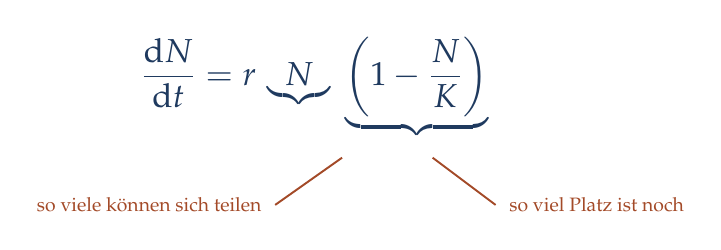
\begin{tikzpicture}[scale=1.0]
\node[font=\large, color=tief] at (0,0) {$\displaystyle \frac{\dd N}{\dd t} = r\,\underbrace{N}_{\ }\;\underbrace{\left(1-\frac{N}{K}\right)}_{\ }$};
\draw[akzent, line width=0.7pt] (0.35,-0.75) -- (-0.5,-1.35);
\node[font=\scriptsize, color=akzent, anchor=east] at (-0.55,-1.35) {so viele können sich teilen};
\draw[akzent, line width=0.7pt] (1.5,-0.75) -- (2.3,-1.35);
\node[font=\scriptsize, color=akzent, anchor=west] at (2.35,-1.35) {so viel Platz ist noch};
\end{tikzpicture}
\end{center}

\schritt{Das Produkt als Funktion von $N$}
\[ \frac{\dd N}{\dd t} = rN - \frac{r}{K}N^2 \]
Das ist eine nach unten geöffnete Parabel in $N$ mit Nullstellen bei $N=0$ und $N=K$.

\begin{center}
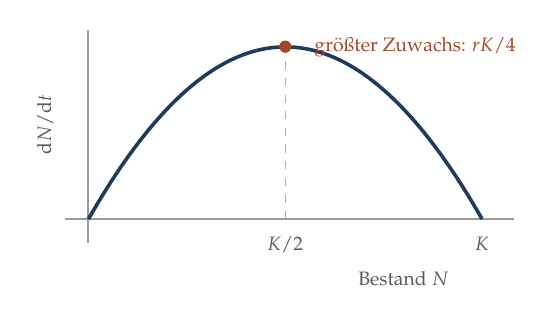
\begin{tikzpicture}[scale=1.0]
\draw[grau!60, line width=0.7pt] (-0.3,0) -- (5.4,0);
\draw[grau!60, line width=0.7pt] (0,-0.3) -- (0,2.4);
\draw[tief, line width=1.3pt, smooth, samples=60, domain=0:5.0]
  plot (\x, {0.35*\x*(5-\x)});
\draw[grau!50, dashed] (2.5,0) -- (2.5,2.19);
\fill[akzent] (2.5,2.19) circle (2.2pt);
\node[font=\scriptsize, color=grau] at (2.5,-0.32) {$K/2$};
\node[font=\scriptsize, color=grau] at (5.0,-0.32) {$K$};
\node[font=\scriptsize, color=akzent, anchor=west] at (2.75,2.19) {größter Zuwachs: $rK/4$};
\node[font=\scriptsize, color=grau, rotate=90] at (-0.55,1.2) {$\dd N/\dd t$};
\node[font=\scriptsize, color=grau] at (4.0,-0.75) {Bestand $N$};
\end{tikzpicture}
\end{center}

\schritt{Der Scheitel}
Eine Parabel mit Nullstellen bei $0$ und $K$ hat ihren Scheitel in der Mitte, also bei $N = K/2$. Der Wert dort:
\[ r\cdot\frac{K}{2}\left(1-\frac12\right) = \frac{rK}{4} . \]

\begin{center}
\begin{minipage}{0.9\textwidth}
\textbf{Der Zuwachs je Zeiteinheit ist am größten, wenn der Bestand die halbe Kapazität erreicht hat.} Vorher sind zu wenige da, nachher ist zu wenig Platz.
\end{minipage}
\end{center}
\end{merksatz}

\section{Die Lösung}

\begin{merksatz}
\boxtitel{Satz 2.2 --- die logistische Funktion}
Die Lösung von Definition 2.1 mit $N(0) = N_0$, wobei $0 < N_0 < K$, lautet
\[ N(t) \;=\; \frac{K}{1 + \left(\dfrac{K-N_0}{N_0}\right)e^{-rt}} . \]
\end{merksatz}

\begin{merksatz}
\boxtitel{Beweis --- Schritt 1 bis 3}
\schritt{Schritt 1 --- Trennen}
\[ \frac{\dd N}{N\left(1-\frac{N}{K}\right)} = r\,\dd t \]

\schritt{Schritt 2 --- Den Bruch zerlegen}
Der Nenner links ist ein Produkt. Solche Brüche zerlegt man in eine Summe --- das ist die \Begriff{Partialbruchzerlegung} (Band 3, Teil~III).

\kursiv{Die Behauptung:}
\[ \frac{1}{N\left(1-\frac{N}{K}\right)} \;=\; \frac{1}{N} + \frac{1/K}{1-\frac{N}{K}} \]

\kursiv{Die Probe} --- rechte Seite auf den gemeinsamen Nenner bringen:
\begin{align*}
\frac{1}{N} + \frac{1/K}{1-\frac{N}{K}} &= \frac{\left(1-\frac{N}{K}\right) + \frac{N}{K}}{N\left(1-\frac{N}{K}\right)}\\
&= \frac{1 - \frac{N}{K} + \frac{N}{K}}{N\left(1-\frac{N}{K}\right)} = \frac{1}{N\left(1-\frac{N}{K}\right)} . \quad \checkmark
\end{align*}

\schritt{Schritt 3 --- Beide Seiten integrieren}
\[ \int\frac{\dd N}{N} + \int\frac{1/K}{1-\frac{N}{K}}\,\dd N = \int r\,\dd t \]

Das erste Integral ist $\ln N$.

Für das zweite setzen wir $u = 1 - \frac{N}{K}$, also $\dd u = -\frac{1}{K}\dd N$ und damit $\frac{1}{K}\dd N = -\dd u$:
\[ \int\frac{1/K}{u}\,\dd N = \int \frac{-\dd u}{u} = -\ln u = -\ln\left(1-\frac{N}{K}\right) . \]

Zusammen:
\[ \ln N - \ln\left(1-\frac{N}{K}\right) = rt + C \]
\[ \ln\frac{N}{1-\frac{N}{K}} = rt + C \]
\end{merksatz}

\begin{merksatz}
\boxtitel{Beweis --- Schritt 4 bis 6}
\schritt{Schritt 4 --- Entlogarithmieren und nach $N$ auflösen}
\[ \frac{N}{1-\frac{N}{K}} = e^{C}e^{rt} =: A\,e^{rt} \]

Mit $1-\frac{N}{K}$ durchmultiplizieren:
\begin{align*}
N &= A\,e^{rt}\left(1-\frac{N}{K}\right)\\
N &= A\,e^{rt} - \frac{A\,e^{rt}}{K}\,N\\
N + \frac{A\,e^{rt}}{K}\,N &= A\,e^{rt}\\
N\left(1 + \frac{A\,e^{rt}}{K}\right) &= A\,e^{rt}\\
N &= \frac{A\,e^{rt}}{1 + \frac{A\,e^{rt}}{K}}
\end{align*}

Zähler und Nenner durch $A\,e^{rt}$ teilen:
\[ N(t) = \frac{1}{\frac{1}{A\,e^{rt}} + \frac{1}{K}} = \frac{K}{\frac{K}{A}\,e^{-rt} + 1} \]

\schritt{Schritt 5 --- Die Konstante bestimmen}
Bei $t=0$:
\[ N_0 = \frac{K}{\frac{K}{A} + 1} \quad\Longrightarrow\quad \frac{K}{A} + 1 = \frac{K}{N_0} \quad\Longrightarrow\quad \frac{K}{A} = \frac{K}{N_0} - 1 = \frac{K-N_0}{N_0} \]

Eingesetzt ergibt sich die Behauptung.

\schritt{Schritt 6 --- Die Probe}
Wir schreiben zur Abkürzung $B = \frac{K-N_0}{N_0}$, also $N = \dfrac{K}{1+Be^{-rt}}$.

\kursiv{Ableiten} mit der Kettenregel:
\[ \frac{\dd N}{\dd t} = K \cdot \left(-1\right)\left(1+Be^{-rt}\right)^{-2}\cdot B\cdot(-r)e^{-rt} = \frac{KrBe^{-rt}}{\left(1+Be^{-rt}\right)^{2}} \]

\kursiv{Die rechte Seite der Gleichung:}
\[ 1 - \frac{N}{K} = 1 - \frac{1}{1+Be^{-rt}} = \frac{1+Be^{-rt}-1}{1+Be^{-rt}} = \frac{Be^{-rt}}{1+Be^{-rt}} \]
\[ rN\left(1-\frac{N}{K}\right) = r\cdot\frac{K}{1+Be^{-rt}}\cdot\frac{Be^{-rt}}{1+Be^{-rt}} = \frac{KrBe^{-rt}}{\left(1+Be^{-rt}\right)^{2}} \]

Beide Seiten stimmen überein. Und $N(0) = \frac{K}{1+B} = \frac{K}{K/N_0} = N_0$. \checkmark\ $\blacksquare$
\end{merksatz}

\section{Was die Kurve tut}

\begin{merksatz}
\boxtitel{Die drei Grenzfälle}
\begin{center}
{\small
\renewcommand{\arraystretch}{1.55}
\begin{tabular}{@{}P{2.6cm}P{6.0cm}@{}}
\toprule
\textbf{$t \to -\infty$} & $e^{-rt} \to \infty$, der Nenner wird groß, $N \to 0$.\\
\textbf{$t \to +\infty$} & $e^{-rt} \to 0$, der Nenner wird $1$, also $N \to K$.\\
\textbf{$N \ll K$} & Der Term $N/K$ ist vernachlässigbar; die Gleichung geht in $\dd N/\dd t = rN$ über --- Kapitel~1.\\
\bottomrule
\end{tabular}}
\end{center}

\begin{center}
\begin{minipage}{0.88\textwidth}
\kursiv{Die dritte Zeile ist die Rechtfertigung von Kapitel~1: Das exponentielle Modell ist der Grenzfall des logistischen bei kleinem Bestand. Es ist nicht falsch, sondern eine Näherung mit angebbarem Gültigkeitsbereich.}
\end{minipage}
\end{center}
\end{merksatz}

\begin{merksatz}
\boxtitel{Satz 2.3 --- der Wendepunkt}
Die logistische Kurve hat ihren Wendepunkt genau bei $N = K/2$, und zwar zur Zeit
\[ t^{*} = \frac{1}{r}\,\ln\frac{K-N_0}{N_0} . \]

\schritt{Beweis --- der Wendepunkt}
Wir leiten die Gleichung nach $t$ ab. Mit $\dd N/\dd t = rN - \frac{r}{K}N^2$:
\[ \frac{\dd^2N}{\dd t^2} = r\frac{\dd N}{\dd t} - \frac{2r}{K}N\frac{\dd N}{\dd t} = \frac{\dd N}{\dd t}\left(r - \frac{2r}{K}N\right) = r\,\frac{\dd N}{\dd t}\left(1 - \frac{2N}{K}\right) \]

Da $0 < N < K$ ist $\dd N/\dd t > 0$, also verschwindet die zweite Ableitung genau dann, wenn
\[ 1 - \frac{2N}{K} = 0 \quad\Longleftrightarrow\quad N = \frac{K}{2} . \]

\schritt{Beweis --- der Zeitpunkt}
Aus der Lösung mit $N = K/2$:
\[ \frac{K}{2} = \frac{K}{1+Be^{-rt^*}} \quad\Longrightarrow\quad 1+Be^{-rt^*} = 2 \quad\Longrightarrow\quad Be^{-rt^*} = 1 \]
\[ e^{-rt^*} = \frac{1}{B} \quad\Longrightarrow\quad -rt^* = -\ln B \quad\Longrightarrow\quad t^* = \frac{\ln B}{r} = \frac{1}{r}\ln\frac{K-N_0}{N_0} . \qquad \blacksquare \]

\begin{center}
\begin{minipage}{0.88\textwidth}
\kursiv{Der Wendepunkt ist der Zeitpunkt des schnellsten Zuwachses. In einer Epidemie entspricht er dem Gipfel der Neuinfektionen --- und er liegt \kursiv{nicht} dort, wo die meisten Menschen erkrankt sind, sondern dort, wo die meisten \kursiv{neu} erkranken. Kapitel~7 kommt darauf zurück.}
\end{minipage}
\end{center}
\end{merksatz}

\section{Die Kultur am Klinikum}

\begin{merksatz}
\boxtitel{Dieselben Zahlen wie in Kapitel~1, mit Grenze}
$N_0 = 10^4$ je Milliliter, $r = 1{,}386\ \mathrm{h}^{-1}$, und als Kapazitätsgrenze $K = 10^9$ je Milliliter.

\schritt{Die Konstante}
\[ B = \frac{K-N_0}{N_0} = \frac{10^9 - 10^4}{10^4} = 10^5 - 1 = 99\,999 \approx 10^5 \]

\schritt{Die Lösung}
\[ N(t) = \frac{10^9}{1 + 99\,999\,e^{-1{,}386\,t}} \]

\schritt{Der Vergleich mit Kapitel~1}
\begin{center}
{\small
\renewcommand{\arraystretch}{1.48}
\begin{tabular}{@{}P{1.4cm}P{2.2cm}P{2.2cm}P{2.0cm}@{}}
\toprule
$t$ (h) & \textbf{exponentiell} & \textbf{logistisch} & \textbf{Abweichung}\\
\midrule
$2$ & $1{,}6\cdot10^{5}$ & $1{,}6\cdot10^{5}$ & \textcolor{gruen}{$<1\,\%$}\\
$4$ & $2{,}56\cdot10^{6}$ & $2{,}55\cdot10^{6}$ & \textcolor{gruen}{$0{,}3\,\%$}\\
$6$ & $4{,}10\cdot10^{7}$ & $3{,}93\cdot10^{7}$ & $4\,\%$\\
$8$ & $6{,}55\cdot10^{8}$ & $3{,}96\cdot10^{8}$ & \textcolor{akzent}{$40\,\%$}\\
$10$ & $1{,}05\cdot10^{10}$ & $8{,}68\cdot10^{8}$ & \textcolor{akzent}{Faktor $12$}\\
$12$ & $1{,}68\cdot10^{11}$ & $9{,}91\cdot10^{8}$ & \textcolor{akzent}{Faktor $169$}\\
\bottomrule
\end{tabular}}
\end{center}

\kursiv{Beispielrechnung für $t=8$:}
\[ e^{-1{,}386\cdot8} = e^{-11{,}09} = 1{,}526\cdot10^{-5} \]
\[ 99\,999 \cdot 1{,}526\cdot10^{-5} = 1{,}526 \]
\[ N(8) = \frac{10^9}{1+1{,}526} = \frac{10^9}{2{,}526} = 3{,}96\cdot10^{8} \]

\schritt{Die Deutung}
\begin{center}
\begin{minipage}{0.9\textwidth}
\textbf{Bis etwa sechs Stunden sind beide Modelle praktisch gleich.} Danach trennen sie sich rasch --- und zwar genau dort, wo der Bestand in die Größenordnung von $K$ kommt.
\end{minipage}
\end{center}

\schritt{Der Wendepunkt}
\[ t^{*} = \frac{\ln 99\,999}{1{,}386} = \frac{11{,}513}{1{,}386} = 8{,}31\ \text{h} \]

Zu diesem Zeitpunkt beträgt der Bestand $5\cdot10^8$, und der Zuwachs ist am größten:
\[ \frac{rK}{4} = \frac{1{,}386\cdot10^9}{4} = 3{,}47\cdot10^{8} \ \text{je Stunde} . \]

\begin{center}
\begin{minipage}{0.88\textwidth}
\kursiv{Die praktische Folgerung für das Labor: Will man die Kultur im gleichmäßigen Wachstum halten --- etwa für einen Empfindlichkeitstest ---, so muss man vor dem Wendepunkt verdünnen. Nach acht Stunden ist die Kultur bereits im Übergang zur Sättigung, und die Zellen verhalten sich anders.}
\end{minipage}
\end{center}
\end{merksatz}

\section{Der Bruchfall}

\begin{warnung}
\boxtitelr{Vier Dinge, die das logistische Modell nicht kann}
\begin{center}
{\small
\renewcommand{\arraystretch}{1.52}
\begin{tabular}{@{}P{2.6cm}P{6.0cm}@{}}
\toprule
\textbf{Anlaufphase} & Die Kurve steigt von Anfang an. Die Verzögerung, bis sich Zellen an ein neues Medium angepasst haben, fehlt.\\
\textbf{Absterben} & Nach der Sättigung bleibt $N = K$ für immer. Das Absterben aus dem Bild in Kapitel~1 kommt nicht vor.\\
\textbf{Symmetrie} & Die Kurve ist punktsymmetrisch zum Wendepunkt --- Aufgabe 2.3. Viele biologische Verläufe sind es nicht.\\
\textbf{Feste Grenze} & $K$ gilt als Konstante. In Wirklichkeit hängt sie von Bedingungen ab, die sich ändern.\\
\bottomrule
\end{tabular}}
\end{center}

\schritt{Zur dritten Zeile}
Die Symmetrie ist die folgenreichste Einschränkung. Beim Tumorwachstum etwa verlangsamt sich das Wachstum \kursiv{früher} als bei halber Endgröße --- das logistische Modell passt dort schlecht.

\begin{center}
\begin{minipage}{0.88\textwidth}
\kursiv{Deshalb benutzt man in der Onkologie meist das Gompertz-Modell, dessen Wendepunkt bei etwa $37\,\%$ der Endgröße liegt --- bei $K/e$, um genau zu sein. Kapitel~13 leitet es her.}
\end{minipage}
\end{center}
\end{warnung}

\begin{merksatz}
\boxtitel{Wie man die Parameter schätzt}
$r$ und $K$ sind selten bekannt; man bestimmt sie aus Daten.

\begin{center}
{\small
\renewcommand{\arraystretch}{1.5}
\begin{tabular}{@{}P{2.4cm}P{6.2cm}@{}}
\toprule
\textbf{$K$ ablesen} & Aus dem Sättigungswert --- setzt voraus, dass man lange genug gemessen hat.\\
\textbf{$r$ aus der Frühphase} & Halblogarithmische Auftragung der frühen Werte; die Steigung ist $r$ (Kapitel~1).\\
\textbf{Beides zugleich} & Nichtlineare Anpassung nach kleinsten Quadraten --- Band 17, Kapitel~10, mit einer nichtlinearen Funktion.\\
\bottomrule
\end{tabular}}
\end{center}

\schritt{Der übliche Fehler}
Schätzt man $K$ aus Daten, die noch weit vor der Sättigung liegen, so ist die Schätzung praktisch beliebig.

\begin{center}
\begin{minipage}{0.88\textwidth}
\kursiv{Das ist bei Epidemien und beim Tumorwachstum der Regelfall: Man hat die aufsteigende Flanke und will die Endgröße vorhersagen. Verschiedene Kurven, die alle gut zu den vorhandenen Daten passen, sagen dann völlig verschiedene Endwerte voraus. Die Unsicherheit ist \kursiv{sehr} viel größer, als die Anpassungsgüte vermuten lässt.}
\end{minipage}
\end{center}

\schritt{Eine Faustregel}
\begin{center}
\begin{minipage}{0.9\textwidth}
\textbf{Vor dem Wendepunkt ist $K$ nicht zuverlässig schätzbar.} Solange die Kurve noch beschleunigt, enthalten die Daten kaum Auskunft über die Grenze.
\end{minipage}
\end{center}
\end{merksatz}

\section{Übungsaufgaben}

\begin{aufgabe}
\boxtitel{Aufgabe 2.1 --- Eine logistische Kurve aufstellen}
Eine Hefekultur startet mit $N_0 = 5$ Einheiten, erreicht als Sättigungswert $K = 665$ Einheiten und hat eine Anfangswachstumsrate von $r = 0{,}54\ \mathrm{h}^{-1}$. Bestimmen Sie die Lösung, den Wendepunkt und den Bestand nach $10$ und $20$ Stunden.

\loesung
\schritt{Schritt 1 --- Die Konstante}
\[ B = \frac{K-N_0}{N_0} = \frac{665-5}{5} = \frac{660}{5} = 132 \]

\schritt{Schritt 2 --- Die Lösung}
\[ N(t) = \frac{665}{1 + 132\,e^{-0{,}54\,t}} \]

\schritt{Schritt 3 --- Der Wendepunkt}
\[ t^{*} = \frac{\ln 132}{0{,}54} = \frac{4{,}883}{0{,}54} = 9{,}04\ \text{h} \]
Dort ist $N = K/2 = 332{,}5$, und der Zuwachs beträgt
\[ \frac{rK}{4} = \frac{0{,}54 \cdot 665}{4} = 89{,}8 \ \text{Einheiten je Stunde} . \]

\schritt{Schritt 4 --- Nach zehn Stunden}
\[ e^{-0{,}54 \cdot 10} = e^{-5{,}40} = 0{,}004517 \]
\[ 132 \cdot 0{,}004517 = 0{,}5962 \]
\[ N(10) = \frac{665}{1{,}5962} = 416{,}6 \]

\schritt{Schritt 5 --- Nach zwanzig Stunden}
\[ e^{-10{,}80} = 2{,}039\cdot10^{-5} \]
\[ 132 \cdot 2{,}039\cdot10^{-5} = 0{,}002692 \]
\[ N(20) = \frac{665}{1{,}002692} = 663{,}2 \]

\schritt{Schritt 6 --- Die Übersicht}
\begin{center}
\renewcommand{\arraystretch}{1.45}
\begin{tabular}{@{}P{1.8cm}P{2.0cm}P{2.6cm}@{}}
\toprule
$t$ (h) & $N(t)$ & \textbf{Anteil an $K$}\\
\midrule
$0$ & $5{,}0$ & $0{,}8\,\%$\\
$5$ & $50{,}5$ & $7{,}6\,\%$\\
$9{,}04$ & $332{,}5$ & $50{,}0\,\%$\\
$10$ & $416{,}6$ & $62{,}6\,\%$\\
$15$ & $632{,}8$ & $95{,}2\,\%$\\
$20$ & $663{,}2$ & $99{,}7\,\%$\\
\bottomrule
\end{tabular}
\end{center}

\schritt{Probe an der Symmetrie}
Der Wendepunkt liegt bei $9{,}04$ h. Nach Aufgabe 2.3 muss gelten
\[ N(t^*-\Delta) + N(t^*+\Delta) = K . \]
Prüfen wir mit $\Delta = 4$ h, also $t = 5{,}04$ und $t = 13{,}04$:
\[ N(5{,}04) = \frac{665}{1+132\,e^{-2{,}722}} = \frac{665}{1+132\cdot0{,}06573} = \frac{665}{9{,}676} = 68{,}7 \]
\[ N(13{,}04) = \frac{665}{1+132\,e^{-7{,}042}} = \frac{665}{1+132\cdot0{,}0008737} = \frac{665}{1{,}1153} = 596{,}3 \]
\[ 68{,}7 + 596{,}3 = 665{,}0 = K . \quad \checkmark \]

\schritt{Eine Bemerkung zu den Zahlen}
Die Werte $N_0 = 5$, $K = 665$, $r = 0{,}54$ stammen aus der klassischen Hefeuntersuchung von Carlson (1913) --- einem der ersten Datensätze, an denen die logistische Kurve geprüft wurde. Sie passt dort außergewöhnlich gut.
\end{aufgabe}

\begin{aufgabe}
\boxtitel{Aufgabe 2.2 --- Wann sind $90$ Prozent erreicht?}
Leiten Sie eine allgemeine Formel für den Zeitpunkt her, zu dem der Bestand einen Anteil $p$ der Kapazität erreicht, und wenden Sie sie auf die Klinikumskultur an.

\loesung
\schritt{Schritt 1 --- Die Bedingung}
\[ N(t_p) = p\,K \quad\Longrightarrow\quad \frac{K}{1+Be^{-rt_p}} = pK \]

\schritt{Schritt 2 --- Auflösen}
\begin{align*}
\frac{1}{1+Be^{-rt_p}} &= p\\
1+Be^{-rt_p} &= \frac{1}{p}\\
Be^{-rt_p} &= \frac{1}{p} - 1 = \frac{1-p}{p}\\
e^{-rt_p} &= \frac{1-p}{p\,B}\\
-rt_p &= \ln\frac{1-p}{p\,B}\\
t_p &= \frac{1}{r}\,\ln\frac{p\,B}{1-p}
\end{align*}

\schritt{Schritt 3 --- Die Formel prüfen}
Für $p = \frac12$ ergibt sich
\[ t_{1/2} = \frac{1}{r}\ln\frac{\frac12 B}{\frac12} = \frac{\ln B}{r} = t^{*} . \quad \checkmark \]
Das stimmt mit Satz 2.3 überein.

\schritt{Schritt 4 --- Anwendung auf die Kultur}
$B = 99\,999$, $r = 1{,}386\ \mathrm{h}^{-1}$.
\begin{center}
{\small
\renewcommand{\arraystretch}{1.45}
\begin{tabular}{@{}P{1.4cm}P{2.6cm}P{2.2cm}P{1.8cm}@{}}
\toprule
$p$ & $\frac{pB}{1-p}$ & $\ln$ & $t_p$ (h)\\
\midrule
$0{,}10$ & $11\,111$ & $9{,}316$ & $6{,}72$\\
$0{,}50$ & $99\,999$ & $11{,}513$ & $8{,}31$\\
$0{,}90$ & $899\,991$ & $13{,}710$ & $9{,}89$\\
$0{,}99$ & $9{,}9\cdot10^{6}$ & $16{,}108$ & $11{,}62$\\
\bottomrule
\end{tabular}}
\end{center}

\schritt{Schritt 5 --- Die Beobachtung}
Von $10$ auf $50$ Prozent dauert es $1{,}59$ Stunden. Von $50$ auf $90$ Prozent ebenfalls $1{,}58$ Stunden.

\begin{center}
\begin{minipage}{0.9\textwidth}
\textbf{Das ist wieder die Symmetrie.} Die Zeitspanne von $p$ bis $\frac12$ ist genauso lang wie die von $\frac12$ bis $1-p$.
\end{minipage}
\end{center}

\schritt{Schritt 6 --- Der Nachweis}
Aus der Formel:
\[ t_{1-p} - t_{1/2} = \frac{1}{r}\left[\ln\frac{(1-p)B}{p} - \ln B\right] = \frac{1}{r}\ln\frac{1-p}{p} \]
\[ t_{1/2} - t_{p} = \frac{1}{r}\left[\ln B - \ln\frac{pB}{1-p}\right] = \frac{1}{r}\ln\frac{1-p}{p} \]
Beide Ausdrücke sind gleich. $\blacksquare$

\begin{center}
\begin{minipage}{0.86\textwidth}
\kursiv{Bemerkenswert ist, dass $B$ dabei herausfällt --- die Spanne hängt also nicht vom Ausgangsbestand ab, sondern nur von $r$. Für die Klinikumskultur: Von zehn auf neunzig Prozent dauert es stets $\frac{2}{r}\ln 9 = \frac{4{,}394}{1{,}386} = 3{,}17$ Stunden, gleichgültig wie klein man beginnt.}
\end{minipage}
\end{center}
\end{aufgabe}

\begin{aufgabe}
\boxtitel{Aufgabe 2.3 --- Die Symmetrie beweisen}
Zeigen Sie, dass die logistische Kurve punktsymmetrisch zu ihrem Wendepunkt ist --- also dass für alle $\Delta$ gilt
\[ N(t^*-\Delta) + N(t^*+\Delta) = K . \]

\loesung
\schritt{Schritt 1 --- Den Wendepunkt einsetzen}
Aus Satz 2.3 ist $e^{-rt^*} = 1/B$, also $B\,e^{-rt^*} = 1$.

\schritt{Schritt 2 --- Die beiden Werte ausdrücken}
\[ N(t^*+\Delta) = \frac{K}{1+Be^{-r(t^*+\Delta)}} = \frac{K}{1+Be^{-rt^*}e^{-r\Delta}} = \frac{K}{1+e^{-r\Delta}} \]
\[ N(t^*-\Delta) = \frac{K}{1+Be^{-rt^*}e^{+r\Delta}} = \frac{K}{1+e^{r\Delta}} \]

\begin{center}
\begin{minipage}{0.88\textwidth}
\kursiv{Beachten Sie, was hier geschehen ist: Durch die Verschiebung auf den Wendepunkt ist $B$ vollständig verschwunden. Die Kurve sieht, vom Wendepunkt aus betrachtet, für jeden Ausgangsbestand gleich aus.}
\end{minipage}
\end{center}

\schritt{Schritt 3 --- Addieren}
Wir schreiben zur Abkürzung $u = e^{r\Delta}$, also $e^{-r\Delta} = 1/u$:
\begin{align*}
N(t^*-\Delta) + N(t^*+\Delta) &= \frac{K}{1+u} + \frac{K}{1+\frac{1}{u}}\\
&= \frac{K}{1+u} + \frac{K\,u}{u+1}\\
&= \frac{K + K\,u}{1+u}\\
&= \frac{K(1+u)}{1+u} \;=\; K . \qquad \blacksquare
\end{align*}

\schritt{Schritt 4 --- Die Deutung}
\begin{center}
\begin{minipage}{0.9\textwidth}
Der Verlauf vor dem Wendepunkt ist das Spiegelbild des Verlaufs danach --- gespiegelt an der Höhe $K/2$.
\end{minipage}
\end{center}

\begin{center}
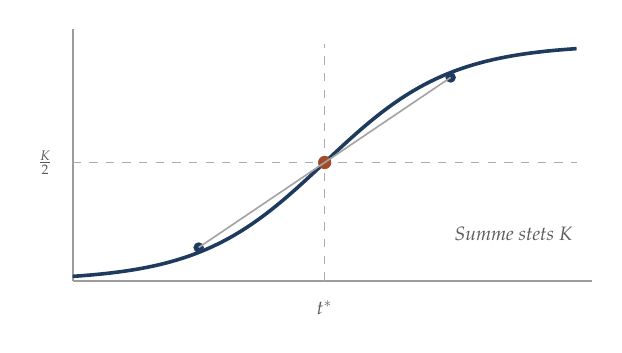
\begin{tikzpicture}[scale=1.0]
\draw[grau!60, line width=0.7pt] (0,0) -- (6.6,0);
\draw[grau!60, line width=0.7pt] (0,0) -- (0,3.2);
\draw[grau!50, dashed] (0,1.5) -- (6.4,1.5);
\draw[grau!50, dashed] (3.2,0) -- (3.2,3.0);
\draw[tief, line width=1.3pt, smooth, samples=70, domain=0:6.4]
  plot (\x, {3.0/(1+exp(-1.25*(\x-3.2)))});
\fill[akzent] (3.2,1.5) circle (2.4pt);
\node[font=\scriptsize, color=grau] at (-0.35,1.5) {$\frac{K}{2}$};
\node[font=\scriptsize, color=grau] at (3.2,-0.35) {$t^{*}$};
\fill[tief] (1.6,0.42) circle (1.9pt);
\fill[tief] (4.8,2.58) circle (1.9pt);
\draw[grau!55, line width=0.6pt] (1.6,0.42) -- (4.8,2.58);
\node[font=\scriptsize\itshape, color=grau] at (5.6,0.6) {Summe stets $K$};
\end{tikzpicture}
\end{center}

\schritt{Schritt 5 --- Warum das eine Einschränkung ist}
Die Symmetrie ist keine Beobachtung, sondern eine \kursiv{Folge des Modells}. Sie wurde nicht aus Daten gewonnen, sondern steckt bereits in der Annahme, dass die Rate \kursiv{linear} mit dem Bestand abnimmt.

\begin{center}
\begin{minipage}{0.86\textwidth}
\kursiv{Wer eine logistische Kurve an Daten anpasst, erzwingt damit die Symmetrie --- auch dann, wenn die Daten sie nicht zeigen. Das ist der Grund, warum man in der Onkologie und bei manchen Epidemien andere Modelle wählt. Kapitel~13 führt die Alternativen vor.}
\end{minipage}
\end{center}
\end{aufgabe}

\begin{geschichte}
\boxtitelg{Ein Name, der zweimal erfunden wurde}
\Person{Pierre-François Verhulst} (1804--1849), belgischer Mathematiker und Schüler von Quetelet, veröffentlichte die Gleichung 1838. Er suchte nach einer Antwort auf Malthus und wollte zeigen, dass das Wachstum einer Bevölkerung an eine Grenze stößt, ohne dass es zur Katastrophe kommen muss.

Verhulst prägte auch den Namen: Er nannte die Kurve \kursiv{logistique}, ohne zu erklären, warum. Über die Herkunft des Wortes wird bis heute gestritten --- am wahrscheinlichsten ist eine Anspielung auf das Logarithmische, das in der Lösung steckt.

\begin{center}
\begin{minipage}{0.9\textwidth}
\kursiv{Verhulst starb mit 45 Jahren, und seine Arbeit geriet vollständig in Vergessenheit. Erst 1920 wurde die Gleichung von \Person{Raymond Pearl} und \Person{Lowell Reed} unabhängig wiederentdeckt, die sie an die Bevölkerungszahlen der Vereinigten Staaten anpassten. Pearl erfuhr erst nachträglich von Verhulsts Arbeit und nannte ihn danach als Urheber.}
\end{minipage}
\end{center}

\schritt{Eine Warnung aus der Geschichte}
Pearl sagte aufgrund seiner Anpassung voraus, die Bevölkerung der Vereinigten Staaten werde sich bei etwa $197$ Millionen einpendeln. Tatsächlich waren es im Jahr 2020 über $330$ Millionen.

\begin{center}
\begin{minipage}{0.9\textwidth}
\kursiv{Der Fehler ist genau der aus dem Abschnitt über die Parameterschätzung: Pearl schätzte $K$ aus Daten, die noch weit vor der Sättigung lagen. Die Anpassung war ausgezeichnet --- und die Hochrechnung falsch. Gute Anpassung an vorhandene Daten sagt nichts über die Güte einer Vorhersage jenseits davon.}
\end{minipage}
\end{center}
\end{geschichte}

\begin{forschung}
\boxtitelp{Wo die logistische Gleichung heute steht}
\begin{center}
{\small
\renewcommand{\arraystretch}{1.45}
\begin{tabular}{@{}P{2.8cm}P{5.4cm}@{}}
\toprule
\textbf{Als Modell} & Für Bakterienkulturen im geschlossenen Gefäß gut brauchbar; für Bevölkerungen und Tumoren meist zu einfach.\\
\textbf{Als Baustein} & In Epidemie- und Ökologiemodellen steckt der Faktor $(1-N/K)$ an vielen Stellen.\\
\textbf{Als Funktion} & Die logistische \kursiv{Funktion} ist von der Gleichung unabhängig geworden: Sie ist die Rückrechnung im logistischen Regressionsmodell (Band 17, Kapitel~11) und die gebräuchlichste Aktivierungsfunktion in neuronalen Netzen.\\
\bottomrule
\end{tabular}}
\end{center}

\begin{center}
\begin{minipage}{0.88\textwidth}
\kursiv{Die dritte Zeile ist bemerkenswert: Dieselbe Funktion entstand in der Bevölkerungslehre, wurde in der Statistik neu entdeckt und ist heute in der Rechnerkunde allgegenwärtig. In keinem der drei Zusammenhänge spielt ihr ursprünglicher Anlass noch eine Rolle.}
\end{minipage}
\end{center}

\schritt{Verallgemeinerungen}
\begin{center}
{\small
\renewcommand{\arraystretch}{1.45}
\begin{tabular}{@{}P{2.4cm}P{5.8cm}@{}}
\toprule
Gompertz & Wendepunkt bei $K/e$; Standard beim Tumorwachstum (Kapitel~13)\\
Richards & Ein zusätzlicher Formparameter verschiebt den Wendepunkt frei\\
Allee-Effekt & Bei sehr kleinem Bestand ist die Rate \kursiv{negativ} --- Partner finden einander nicht mehr\\
\bottomrule
\end{tabular}}
\end{center}

Die letzte Zeile ist für den Artenschutz folgenreich: Unterhalb einer Schwelle stirbt eine Population aus, auch wenn genügend Lebensraum vorhanden wäre. Das logistische Modell kennt diese Schwelle nicht --- bei ihm erholt sich jeder noch so kleine Bestand.
\end{forschung}

\begin{merksatz}
\boxtitel{Was Sie jetzt können}
\begin{center}
\renewcommand{\arraystretch}{1.5}
\begin{tabular}{@{}P{3.0cm}P{5.6cm}@{}}
\toprule
\textbf{Definition 2.1} & ein Faktor mehr als Kapitel~1\\
\textbf{Satz 2.2} & Lösung über Partialbruchzerlegung, mit Probe\\
\textbf{Satz 2.3} & Wendepunkt bei $K/2$, größter Zuwachs $rK/4$\\
\textbf{Die Symmetrie} & eine Folge des Modells, keine Beobachtung\\
\textbf{Der Bruchfall} & $K$ ist vor dem Wendepunkt nicht schätzbar\\
\bottomrule
\end{tabular}
\end{center}

\begin{center}
\begin{minipage}{0.88\textwidth}
\kursiv{Im nächsten Kapitel lassen wir die Zeit in Sprüngen statt stetig verlaufen --- und dieselbe Gleichung verhält sich plötzlich völlig anders.}
\end{minipage}
\end{center}
\end{merksatz}

\chapter{Diskrete Modelle und Chaos}

\section{Wenn die Zeit springt}

\begin{merksatz}
\boxtitel{Wann stetige Modelle nicht passen}
Die Kapitel~1 und 2 setzen voraus, dass sich der Bestand ununterbrochen ändert. Bei einer Bakterienkultur trifft das zu --- in jedem Augenblick teilt sich irgendwo eine Zelle.

Bei anderen Populationen ist das anders:

\begin{center}
{\small
\renewcommand{\arraystretch}{1.5}
\begin{tabular}{@{}P{2.6cm}P{6.0cm}@{}}
\toprule
\textbf{Insekten} & Eine Generation je Jahr. Die Elterngeneration ist tot, bevor die nächste schlüpft.\\
\textbf{Jahreszeitliche Vermehrung} & Fische, Vögel, einjährige Pflanzen.\\
\textbf{Messung in Schritten} & Auch bei stetigem Vorgang misst man täglich oder wöchentlich.\\
\bottomrule
\end{tabular}}
\end{center}

\begin{center}
\begin{minipage}{0.9\textwidth}
In solchen Fällen fragt man nicht nach $\dd N/\dd t$, sondern nach einer \Begriff{Rekursion}: Wie hängt die nächste Generation von der jetzigen ab?
\end{minipage}
\end{center}
\end{merksatz}

\begin{definition}
\boxtitelm{Definition 3.1 --- die logistische Abbildung}
Sei $x_n \in [0,1]$ der Bestand der $n$-ten Generation, gemessen als Anteil der Kapazitätsgrenze. Dann ist
\[ x_{n+1} \;=\; a\,x_n\,(1-x_n) \]
mit dem Parameter $a > 0$.
\end{definition}

\begin{merksatz}
\boxtitel{Dieselbe Idee wie in Kapitel 2}
\begin{center}
\renewcommand{\arraystretch}{1.5}
\begin{tabular}{@{}P{2.2cm}P{2.8cm}P{3.0cm}@{}}
\toprule
& \textbf{stetig} & \textbf{diskret}\\
\midrule
Vermehrung & $rN$ & $a\,x_n$\\
Hemmung & $(1-N/K)$ & $(1-x_n)$\\
\bottomrule
\end{tabular}
\end{center}

\begin{center}
\begin{minipage}{0.88\textwidth}
\kursiv{Die Bauweise ist dieselbe: ein Vermehrungsfaktor, gedämpft durch den freien Platz. Man würde erwarten, dass sich die diskrete Fassung ähnlich verhält wie die stetige. Dieses Kapitel handelt davon, dass das grob falsch ist.}
\end{minipage}
\end{center}

\schritt{Warum $x$ ein Anteil ist}
Man rechnet in Einheiten der Kapazitätsgrenze, also $x = N/K$. Das spart einen Parameter: Statt $r$ und $K$ bleibt nur $a$ übrig. Für $x > 1$ wird $x_{n+1}$ negativ --- die Population stirbt aus. Wir bleiben daher in $[0,1]$, was für $0 < a \le 4$ gesichert ist.
\end{merksatz}

\section{Ruhelagen}

\begin{definition}
\boxtitelm{Definition 3.2 --- Fixpunkt}
Ein \Begriff{Fixpunkt} der Abbildung $f$ ist ein Wert $x^{*}$ mit $f(x^{*}) = x^{*}$ --- der Bestand ändert sich von einer Generation zur nächsten nicht.
\end{definition}

\begin{merksatz}
\boxtitel{Satz 3.3 --- die beiden Fixpunkte}
Die logistische Abbildung hat genau die Fixpunkte
\[ x^{*}_1 = 0 \qquad\text{und}\qquad x^{*}_2 = 1 - \frac{1}{a} . \]

\schritt{Beweis}
\begin{align*}
a\,x(1-x) &= x\\
a\,x(1-x) - x &= 0\\
x\bigl[a(1-x) - 1\bigr] &= 0
\end{align*}
Ein Produkt ist null, wenn ein Faktor null ist:
\[ x = 0 \qquad\text{oder}\qquad a(1-x) = 1 \;\Longleftrightarrow\; 1-x = \frac1a \;\Longleftrightarrow\; x = 1-\frac1a . \quad \blacksquare \]

\schritt{Die Bedingung für den zweiten}
$x^{*}_2$ liegt nur dann in $[0,1]$, wenn $a \ge 1$. Für $a < 1$ gibt es nur den Nullpunkt --- die Population stirbt aus.
\end{merksatz}

\begin{merksatz}
\boxtitel{Satz 3.4 --- wann ein Fixpunkt stabil ist}
Ein Fixpunkt $x^{*}$ heißt \Begriff{stabil}, wenn Bestände in seiner Nähe zu ihm hinstreben. Das ist genau dann der Fall, wenn
\[ \bigl|f'(x^{*})\bigr| < 1 . \]

\schritt{Begründung}
Sei $x_n = x^{*} + \varepsilon_n$ mit kleinem $\varepsilon_n$. Dann ist
\[ x_{n+1} = f(x^{*}+\varepsilon_n) \approx f(x^{*}) + f'(x^{*})\,\varepsilon_n = x^{*} + f'(x^{*})\,\varepsilon_n \]
nach der Näherung durch die Tangente (Band 3, Teil~II). Also
\[ \varepsilon_{n+1} \approx f'(x^{*})\,\varepsilon_n . \]

\begin{center}
\begin{minipage}{0.9\textwidth}
Die Abweichung wird in jedem Schritt mit demselben Faktor multipliziert. Ist sein Betrag kleiner als eins, schrumpft sie; ist er größer, wächst sie.
\end{minipage}
\end{center}

\begin{center}
\begin{minipage}{0.88\textwidth}
\kursiv{Das ist wieder exponentielles Verhalten --- nur diesmal für den \kursiv{Fehler} statt für den Bestand. Dieselbe Rechnung wie in Kapitel~1, an einer ganz anderen Stelle.}
\end{minipage}
\end{center}
\end{merksatz}

\begin{merksatz}
\boxtitel{Die Stabilität der beiden Fixpunkte}
\schritt{Die Ableitung}
\[ f(x) = a\,x - a\,x^2 \quad\Longrightarrow\quad f'(x) = a - 2a\,x = a\,(1-2x) \]

\schritt{Am Nullpunkt}
\[ f'(0) = a \]
Stabil für $a < 1$. Die Population stirbt dann aus, gleichgültig wie sie startet.

\schritt{Am zweiten Fixpunkt}
\[ f'\!\left(1-\frac1a\right) = a\left(1 - 2\left(1-\frac1a\right)\right) = a\left(1 - 2 + \frac2a\right) = a\left(\frac2a - 1\right) = 2 - a \]

Stabil, wenn $|2-a| < 1$, also
\[ -1 < 2-a < 1 \quad\Longleftrightarrow\quad 1 < a < 3 . \]

\begin{center}
\begin{minipage}{0.9\textwidth}
\textbf{Bei $a = 3$ verliert der Fixpunkt seine Stabilität.} Was dann geschieht, ist der Gegenstand dieses Kapitels.
\end{minipage}
\end{center}
\end{merksatz}

\begin{merksatz}
\boxtitel{Ein Beispiel: $a = 2{,}8$}
Fixpunkt: $1 - 1/2{,}8 = 0{,}642857$. Ableitung dort: $2 - 2{,}8 = -0{,}8$, Betrag kleiner eins --- stabil.

Start bei $x_0 = 0{,}1$:
\begin{center}
{\small
\renewcommand{\arraystretch}{1.38}
\begin{tabular}{@{}P{1.0cm}P{1.8cm}P{1.0cm}P{1.8cm}@{}}
\toprule
$n$ & $x_n$ & $n$ & $x_n$\\
\midrule
$0$ & $0{,}100000$ & $6$ & $0{,}612166$\\
$1$ & $0{,}252000$ & $7$ & $0{,}664773$\\
$2$ & $0{,}527789$ & $8$ & $0{,}623980$\\
$3$ & $0{,}697838$ & $10$ & $0{,}631017$\\
$4$ & $0{,}590409$ & $12$ & $0{,}635363$\\
$5$ & $0{,}677114$ & $\infty$ & $\mathbf{0{,}642857}$\\
\bottomrule
\end{tabular}}
\end{center}

\begin{center}
\begin{minipage}{0.88\textwidth}
\kursiv{Die Werte springen abwechselnd über und unter den Fixpunkt und nähern sich ihm. Das entspricht dem \kursiv{negativen} Vorzeichen der Ableitung: Jede Abweichung wechselt das Vorzeichen und schrumpft um den Faktor $0{,}8$.}
\end{minipage}
\end{center}
\end{merksatz}

\section{Periodenverdopplung}

\begin{merksatz}
\boxtitel{Was bei $a > 3$ geschieht}
Der Fixpunkt ist instabil. Statt sich einzupendeln, springt der Bestand zwischen \kursiv{zwei} Werten hin und her.

\schritt{Ein Beispiel: $a = 3{,}2$, Start bei $x_0 = 0{,}5$}
Nach einigen Schritten:
\[ \ldots,\ 0{,}799456,\ 0{,}513044,\ 0{,}799455,\ 0{,}513044,\ 0{,}799455,\ \ldots \]

\schritt{Die beiden Werte exakt}
Man sucht Lösungen von $f(f(x)) = x$, die keine Fixpunkte sind. Das führt auf eine quadratische Gleichung mit der Lösung
\[ x = \frac{a+1 \pm \sqrt{(a-3)(a+1)}}{2a} . \]
Für $a = 3{,}2$:
\[ \sqrt{0{,}2 \cdot 4{,}2} = \sqrt{0{,}84} = 0{,}91652 \]
\[ x = \frac{4{,}2 \pm 0{,}91652}{6{,}4} = 0{,}799455 \quad\text{und}\quad 0{,}513045 . \quad \checkmark \]

\begin{center}
\begin{minipage}{0.88\textwidth}
\kursiv{Unter der Wurzel steht $(a-3)(a+1)$. Für $a < 3$ ist der erste Faktor negativ --- es gibt keinen Zweierzyklus. Bei $a = 3$ entsteht er, und zwar genau dort, wo der Fixpunkt seine Stabilität verliert. Die Schwelle ist dieselbe.}
\end{minipage}
\end{center}
\end{merksatz}

\begin{merksatz}
\boxtitel{Und weiter}
Erhöht man $a$ weiter, so wird auch der Zweierzyklus instabil und teilt sich in einen Viererzyklus, dieser in einen Achterzyklus, und so fort.

\begin{center}
{\small
\renewcommand{\arraystretch}{1.48}
\begin{tabular}{@{}P{2.4cm}P{2.4cm}P{2.6cm}@{}}
\toprule
\textbf{Schwelle} & \textbf{Wert von $a$} & \textbf{danach}\\
\midrule
$a_1$ & $3{,}000000$ & Zweierzyklus\\
$a_2$ & $3{,}449490$ & Viererzyklus\\
$a_3$ & $3{,}544090$ & Achterzyklus\\
$a_4$ & $3{,}564407$ & Sechzehner\\
$\vdots$ & $\vdots$ & $\vdots$\\
$a_\infty$ & $\mathbf{3{,}569946}$ & \textcolor{akzent}{\textbf{Chaos}}\\
\bottomrule
\end{tabular}}
\end{center}

Der Wert $a_2 = 1+\sqrt6 = 3{,}44949$ lässt sich noch geschlossen angeben; die weiteren nicht.

\schritt{Die Abstände schrumpfen}
\begin{center}
\renewcommand{\arraystretch}{1.45}
\begin{tabular}{@{}P{2.8cm}P{2.2cm}P{2.6cm}@{}}
\toprule
\textbf{Abstand} & \textbf{Wert} & \textbf{Verhältnis}\\
\midrule
$a_2 - a_1$ & $0{,}449490$ & \\
$a_3 - a_2$ & $0{,}094600$ & $4{,}751$\\
$a_4 - a_3$ & $0{,}020317$ & $4{,}656$\\
$a_5 - a_4$ & $0{,}004351$ & $4{,}669$\\
\bottomrule
\end{tabular}
\end{center}

\begin{center}
\begin{minipage}{0.9\textwidth}
\textbf{Die Verhältnisse streben gegen $\delta = 4{,}669201\ldots$ --- die Feigenbaum-Konstante.}
\end{minipage}
\end{center}

\begin{center}
\begin{minipage}{0.88\textwidth}
\kursiv{Das Bemerkenswerte daran: Diese Zahl hängt \kursiv{nicht} von der logistischen Abbildung ab. Jede Abbildung mit einem glatten Höchstwert zeigt dieselbe Konstante --- ob man $ax(1-x)$ nimmt, $a\sin(\pi x)$ oder etwas ganz anderes. Sie ist eine Naturkonstante der Mathematik, vergleichbar mit $\pi$, und wurde 1975 entdeckt.}
\end{minipage}
\end{center}
\end{merksatz}

\section{Chaos}

\begin{merksatz}
\boxtitel{Jenseits der Häufungsstelle}
Für $a > 3{,}5699$ wiederholt sich die Folge nicht mehr. Sie bleibt beschränkt, springt aber unregelmäßig und ohne erkennbares Muster.

\schritt{Der entscheidende Versuch}
Wir rechnen mit $a = 3{,}9$ zweimal --- einmal mit $x_0 = 0{,}400$, einmal mit $x_0 = 0{,}401$. Der Unterschied im Startwert beträgt ein Promille.

\begin{center}
{\small
\renewcommand{\arraystretch}{1.4}
\begin{tabular}{@{}P{1.0cm}P{2.0cm}P{2.0cm}P{2.0cm}@{}}
\toprule
$n$ & $x_0 = 0{,}400$ & $x_0 = 0{,}401$ & \textbf{Differenz}\\
\midrule
$0$ & $0{,}400000$ & $0{,}401000$ & $0{,}001000$\\
$1$ & $0{,}936000$ & $0{,}936776$ & $0{,}000776$\\
$2$ & $0{,}233626$ & $0{,}230984$ & $0{,}002642$\\
$3$ & $0{,}698274$ & $0{,}692758$ & $0{,}005516$\\
$4$ & $0{,}821681$ & $0{,}830093$ & $0{,}008412$\\
$5$ & $0{,}571434$ & $0{,}550052$ & $0{,}021383$\\
$10$ & $0{,}121805$ & $0{,}140343$ & $0{,}018538$\\
$15$ & $0{,}933177$ & $0{,}913481$ & $0{,}019696$\\
$20$ & $0{,}890718$ & $\mathbf{0{,}125669}$ & \textcolor{akzent}{$\mathbf{0{,}765048}$}\\
\bottomrule
\end{tabular}}
\end{center}

\begin{center}
\begin{minipage}{0.9\textwidth}
\textbf{Nach zwanzig Generationen haben die beiden Verläufe nichts mehr miteinander zu tun.} Der eine liegt nahe am oberen Rand, der andere am unteren.
\end{minipage}
\end{center}
\end{merksatz}

\begin{merksatz}
\boxtitel{Was das bedeutet}
\begin{center}
{\small
\renewcommand{\arraystretch}{1.55}
\begin{tabular}{@{}P{2.6cm}P{6.0cm}@{}}
\toprule
\textbf{Nicht zufällig} & Die Gleichung ist vollständig bestimmt. Bei exakt gleichem Startwert kommt exakt dieselbe Folge heraus.\\
\textbf{Trotzdem unvorhersagbar} & Jeder gemessene Startwert hat einen Fehler. Nach genügend vielen Schritten ist die Vorhersage wertlos.\\
\textbf{Nicht kompliziert} & Die Gleichung hat drei Zeichen. Die Unvorhersagbarkeit entsteht nicht aus Kompliziertheit.\\
\bottomrule
\end{tabular}}
\end{center}

\schritt{Die Rechnung dazu}
Der Fehler wächst im Mittel exponentiell:
\[ \varepsilon_n \approx \varepsilon_0\,e^{\lambda n} \]
mit dem \Begriff{Lyapunow-Exponenten} $\lambda$. Für $a = 3{,}9$ ist $\lambda \approx 0{,}5$.

Ein Anfangsfehler von $10^{-3}$ erreicht die Größenordnung $1$ nach
\[ n \approx \frac{\ln(10^{3})}{0{,}5} = \frac{6{,}91}{0{,}5} \approx 14 \ \text{Schritten} . \]
Das passt zur Tabelle.

\schritt{Was zehnmal genauere Messung brächte}
\[ n \approx \frac{\ln(10^{4})}{0{,}5} = 18{,}4 \]
Vier Schritte mehr. Für weitere vier Schritte bräuchte man wieder zehnmal genauere Messung.

\begin{center}
\begin{minipage}{0.9\textwidth}
\textbf{Der Vorhersagehorizont wächst nur logarithmisch mit der Messgenauigkeit.} Das ist der Grund, warum die Wettervorhersage bei etwa zwei Wochen an eine Grenze stößt, die sich durch bessere Messungen nicht wesentlich verschieben lässt.
\end{minipage}
\end{center}
\end{merksatz}

\begin{warnung}
\boxtitelr{Drei Fehldeutungen}
\begin{center}
{\small
\renewcommand{\arraystretch}{1.52}
\begin{tabular}{@{}P{2.8cm}P{5.8cm}@{}}
\toprule
\textbf{\enquote{Chaos heißt Unordnung}} & Nein. Die Folge bleibt in $[0,1]$, und ihre Häufigkeitsverteilung ist völlig regelmäßig. Ungeordnet ist nur die \kursiv{Reihenfolge}.\\
\textbf{\enquote{Chaos heißt Zufall}} & Nein. Es gibt keinen Zufall in der Gleichung. Die Folge ist vollständig bestimmt.\\
\textbf{\enquote{Mehr Rechenleistung hilft}} & Nein. Das Problem liegt im Startwert, nicht in der Rechnung.\\
\bottomrule
\end{tabular}}
\end{center}

\begin{center}
\begin{minipage}{0.88\textwidth}
\kursiv{Die erste Zeile lohnt eine Bemerkung: Über lange Zeit lässt sich sehr wohl etwas vorhersagen --- nämlich die Verteilung der Werte. Man kann sagen, wie oft die Population klein sein wird, nur nicht wann. Das ist die statistische Betrachtungsweise eines chaotischen Systems, und sie ist oft die einzig sinnvolle.}
\end{minipage}
\end{center}
\end{warnung}

\section{Der Bruchfall}

\begin{warnung}
\boxtitelr{Wann tritt das in der Biologie wirklich auf?}
Die Frage ist berechtigt: Beobachtet man chaotische Populationen?

\begin{center}
{\small
\renewcommand{\arraystretch}{1.5}
\begin{tabular}{@{}P{2.6cm}P{6.0cm}@{}}
\toprule
\textbf{Im Labor} & Bei Mehlkäfern und Wasserflöhen wurden Verläufe gefunden, die zu chaotischen Modellen passen.\\
\textbf{Im Freiland} & Sehr schwer nachzuweisen --- man bräuchte lange, genaue Zeitreihen und müsste Chaos von Zufallsschwankungen trennen.\\
\textbf{Die Parameterwerte} & Chaos verlangt $a > 3{,}57$, also eine Vermehrung um mehr als das Dreieinhalbfache je Generation. Das ist bei Wirbeltieren unmöglich, bei Insekten gut denkbar.\\
\bottomrule
\end{tabular}}
\end{center}

\schritt{Die ehrliche Auskunft}
\begin{center}
\begin{minipage}{0.9\textwidth}
Der Nachweis von Chaos in freilebenden Populationen ist bis heute umstritten. Die Bedeutung dieses Kapitels liegt nicht in der Anwendung, sondern in der \kursiv{Warnung}.
\end{minipage}
\end{center}

\begin{center}
\begin{minipage}{0.88\textwidth}
\kursiv{Die Warnung lautet: Ein unregelmäßiger Verlauf in Daten muss keine äußere Störung haben. Er kann aus dem System selbst stammen. Wer bei schwankenden Populationszahlen nach der Ursache jeder einzelnen Schwankung sucht, sucht unter Umständen etwas, das es nicht gibt.}
\end{minipage}
\end{center}
\end{warnung}

\begin{warnung}
\boxtitelr{Und eine zweite Warnung: die Diskretisierung selbst}
Vergleichen wir für dieselbe biologische Lage:

\begin{center}
\renewcommand{\arraystretch}{1.48}
\begin{tabular}{@{}P{2.8cm}P{2.4cm}P{2.6cm}@{}}
\toprule
& \textbf{stetig} & \textbf{diskret}\\
\midrule
Verhalten & stets Sättigung & \textcolor{akzent}{Zyklen, Chaos}\\
Abhängig von $r$ bzw. $a$ & \textcolor{gruen}{nein} & \textcolor{akzent}{\textbf{ja}}\\
\bottomrule
\end{tabular}
\end{center}

\begin{center}
\begin{minipage}{0.9\textwidth}
\textbf{Die stetige logistische Gleichung strebt für \kursiv{jedes} $r > 0$ gegen $K$. Die diskrete tut das nur für $a < 3$.}
\end{minipage}
\end{center}

\schritt{Woher der Unterschied kommt}
Im stetigen Modell wirkt die Hemmung \kursiv{sofort}. Im diskreten wirkt sie mit einer Generation Verzögerung: Die Nachkommenzahl richtet sich nach dem Bestand der \kursiv{vorigen} Generation.

\begin{center}
\begin{minipage}{0.88\textwidth}
\kursiv{Diese Verzögerung ist die Ursache des Überschwingens --- und damit der Zyklen und des Chaos. Man kann dasselbe im stetigen Modell erzeugen, indem man eine Zeitverzögerung einbaut. \textbf{Verzögerte Rückkopplung erzeugt Schwingungen.} Das ist ein allgemeines Prinzip, das in Teil~II und in der Regelungstechnik wiederkehrt.}
\end{minipage}
\end{center}

\schritt{Die praktische Folgerung}
Wer ein stetiges Modell für die Rechnung in Zeitschritte zerlegt, muss die Schrittweite klein genug wählen. Zu große Schritte erzeugen Schwingungen, die im Modell gar nicht stecken.

\begin{center}
\begin{minipage}{0.88\textwidth}
\kursiv{Das ist kein theoretisches Problem. Ein numerisch gelöstes Modell mit zu grober Schrittweite kann Epidemiewellen oder Populationszyklen zeigen, die reine Rechenartefakte sind. Band 5 behandelt, wie man das erkennt und vermeidet.}
\end{minipage}
\end{center}
\end{warnung}

\section{Übungsaufgaben}

\begin{aufgabe}
\boxtitel{Aufgabe 3.1 --- Fixpunkte und Stabilität}
Untersuchen Sie die Abbildung $x_{n+1} = a\,x_n(1-x_n)$ für $a = 0{,}8$, $a = 2{,}0$ und $a = 3{,}5$.

\loesung
\schritt{$a = 0{,}8$}
Fixpunkte: $x^{*}_1 = 0$ und $x^{*}_2 = 1 - 1/0{,}8 = 1 - 1{,}25 = -0{,}25$.

Der zweite liegt außerhalb von $[0,1]$ und ist biologisch bedeutungslos.

Stabilität von $x^{*}_1 = 0$: $f'(0) = a = 0{,}8 < 1$ --- \textbf{stabil}.

\kursiv{Deutung:} Die Population stirbt aus. Jede Generation erzeugt weniger als eine Nachfolgerin je Individuum, auch bei maximalem freien Platz.

\schritt{$a = 2{,}0$}
Fixpunkte: $0$ und $1 - 1/2 = 0{,}5$.

$f'(0) = 2 > 1$ --- instabil.\\
$f'(0{,}5) = 2 - 2 = 0$ --- \textbf{stabil}, und zwar in besonderem Maße.

\kursiv{Probe mit $x_0 = 0{,}1$:}
\[ 0{,}1 \to 0{,}18 \to 0{,}2952 \to 0{,}41611 \to 0{,}48593 \to 0{,}49960 \to 0{,}5000 \]
Sehr rasche Annäherung, ohne Überschwingen.

\begin{center}
\begin{minipage}{0.86\textwidth}
\kursiv{Die Ableitung null bedeutet \Begriff{überstabil}: Der Fehler wird nicht nur kleiner, sondern quadriert sich. Aus $0{,}01$ wird etwa $0{,}0001$. Das ist die schnellstmögliche Annäherung.}
\end{minipage}
\end{center}

\schritt{$a = 3{,}5$}
Fixpunkt: $1 - 1/3{,}5 = 0{,}714286$.

$f'(0{,}714286) = 2 - 3{,}5 = -1{,}5$, Betrag größer als eins --- \textbf{instabil}.

Da $3{,}449 < 3{,}5 < 3{,}544$, liegt nach der Tabelle in Abschnitt 3.3 ein \textbf{Viererzyklus} vor.

\kursiv{Probe:} Die vier Werte lauten näherungsweise
\[ 0{,}500884,\quad 0{,}874997,\quad 0{,}382820,\quad 0{,}826941 \]
und wiederholen sich danach.

\schritt{Die Übersicht}
\begin{center}
\renewcommand{\arraystretch}{1.48}
\begin{tabular}{@{}P{1.4cm}P{2.4cm}P{2.0cm}P{2.4cm}@{}}
\toprule
$a$ & \textbf{stabiler Zustand} & $|f'|$ & \textbf{Verhalten}\\
\midrule
$0{,}8$ & $x=0$ & $0{,}8$ & Aussterben\\
$2{,}0$ & $x=0{,}5$ & $0$ & rasche Sättigung\\
$3{,}5$ & \textcolor{akzent}{keiner} & $1{,}5$ & Viererzyklus\\
\bottomrule
\end{tabular}
\end{center}
\end{aufgabe}

\begin{aufgabe}
\boxtitel{Aufgabe 3.2 --- Den Zweierzyklus herleiten}
Zeigen Sie, dass die Werte des Zweierzyklus
\[ x = \frac{a+1 \pm \sqrt{(a-3)(a+1)}}{2a} \]
lauten, und bestimmen Sie, ab welchem $a$ er existiert.

\loesung
\schritt{Schritt 1 --- Die Bedingung}
Ein Zweierzyklus besteht aus zwei Werten $p$ und $q$ mit
\[ f(p) = q \qquad\text{und}\qquad f(q) = p , \]
also $f(f(p)) = p$. Wir suchen die Fixpunkte der zweifach angewandten Abbildung.

\schritt{Schritt 2 --- Ein Kunstgriff}
Statt $f(f(x)) = x$ auszumultiplizieren --- das gäbe ein Polynom vierten Grades ---, nutzen wir zwei Beziehungen aus. Aus
\[ q = ap(1-p) \qquad\text{und}\qquad p = aq(1-q) \]
folgt durch Addition und Subtraktion Handlicheres.

\kursiv{Subtraktion:}
\begin{align*}
q - p &= ap(1-p) - aq(1-q)\\
&= a\bigl[p - p^2 - q + q^2\bigr]\\
&= a\bigl[(p-q) - (p^2-q^2)\bigr]\\
&= a(p-q)\bigl[1 - (p+q)\bigr]
\end{align*}
Da $p \neq q$, dürfen wir durch $(q-p) = -(p-q)$ teilen:
\[ 1 = -a\bigl[1-(p+q)\bigr] \quad\Longrightarrow\quad p+q = 1 + \frac{1}{a} = \frac{a+1}{a} . \]

\schritt{Schritt 3 --- Das Produkt}
\kursiv{Addition:}
\[ p+q = a\bigl[(p+q) - (p^2+q^2)\bigr] \]
Mit $p^2+q^2 = (p+q)^2 - 2pq$ und $S := p+q = \frac{a+1}{a}$:
\[ S = a\bigl[S - S^2 + 2pq\bigr] \]
\[ \frac{S}{a} = S - S^2 + 2pq \quad\Longrightarrow\quad 2pq = \frac{S}{a} - S + S^2 \]

Einsetzen von $S = \frac{a+1}{a}$:
\[ 2pq = \frac{a+1}{a^2} - \frac{a+1}{a} + \frac{(a+1)^2}{a^2} = \frac{(a+1) - a(a+1) + (a+1)^2}{a^2} \]
\[ = \frac{(a+1)\bigl[1 - a + a + 1\bigr]}{a^2} = \frac{2(a+1)}{a^2} \]
\[ P := pq = \frac{a+1}{a^2} \]

\schritt{Schritt 4 --- Die quadratische Gleichung}
$p$ und $q$ sind die Lösungen von $x^2 - Sx + P = 0$:
\[ x = \frac{S \pm \sqrt{S^2 - 4P}}{2} \]

\kursiv{Die Diskriminante:}
\[ S^2 - 4P = \frac{(a+1)^2}{a^2} - \frac{4(a+1)}{a^2} = \frac{(a+1)\bigl[(a+1)-4\bigr]}{a^2} = \frac{(a+1)(a-3)}{a^2} \]

\[ x = \frac{\frac{a+1}{a} \pm \frac{\sqrt{(a+1)(a-3)}}{a}}{2} = \frac{a+1 \pm \sqrt{(a-3)(a+1)}}{2a} . \qquad \blacksquare \]

\schritt{Schritt 5 --- Wann er existiert}
Die Wurzel ist genau dann reell, wenn $(a-3)(a+1) \ge 0$. Für $a > 0$ ist $a+1 > 0$, also
\[ a \ge 3 . \]

\begin{center}
\begin{minipage}{0.9\textwidth}
\textbf{Der Zweierzyklus entsteht genau dort, wo der Fixpunkt seine Stabilität verliert.} Beide Schwellen liegen bei $a = 3$.
\end{minipage}
\end{center}

\schritt{Probe für $a = 3{,}2$}
\[ S = \frac{4{,}2}{3{,}2} = 1{,}3125, \qquad P = \frac{4{,}2}{10{,}24} = 0{,}410156 \]
\[ p + q = 0{,}513045 + 0{,}799455 = 1{,}312500 \quad \checkmark \]
\[ p \cdot q = 0{,}513045 \cdot 0{,}799455 = 0{,}410156 \quad \checkmark \]
\end{aufgabe}

\begin{aufgabe}
\boxtitel{Aufgabe 3.3 --- Wie weit reicht eine Vorhersage?}
Ein chaotisches System hat den Lyapunow-Exponenten $\lambda = 0{,}5$ je Schritt. Der Startwert ist auf drei Stellen genau bekannt. Nach wie vielen Schritten ist die Vorhersage wertlos? Wie viel brächte eine Messung auf sechs Stellen?

\loesung
\schritt{Schritt 1 --- Die Bedingung}
Der Fehler wächst wie $\varepsilon_n = \varepsilon_0\,e^{\lambda n}$. Die Vorhersage ist wertlos, wenn er die Größenordnung des Wertebereichs erreicht --- hier etwa $1$.

\[ \varepsilon_0\,e^{\lambda n} \approx 1 \quad\Longrightarrow\quad e^{\lambda n} \approx \frac{1}{\varepsilon_0} \quad\Longrightarrow\quad n \approx \frac{1}{\lambda}\ln\frac{1}{\varepsilon_0} \]

\schritt{Schritt 2 --- Drei Stellen}
$\varepsilon_0 = 10^{-3}$:
\[ n \approx \frac{\ln 10^3}{0{,}5} = \frac{6{,}908}{0{,}5} = 13{,}8 \approx 14 \ \text{Schritte} \]

\schritt{Schritt 3 --- Sechs Stellen}
$\varepsilon_0 = 10^{-6}$:
\[ n \approx \frac{\ln 10^6}{0{,}5} = \frac{13{,}816}{0{,}5} = 27{,}6 \approx 28 \ \text{Schritte} \]

\schritt{Schritt 4 --- Der Vergleich}
\begin{center}
\renewcommand{\arraystretch}{1.48}
\begin{tabular}{@{}P{2.4cm}P{2.4cm}P{2.8cm}@{}}
\toprule
\textbf{Genauigkeit} & \textbf{Faktor} & \textbf{Horizont}\\
\midrule
$10^{-3}$ & $1$ & $14$ Schritte\\
$10^{-6}$ & $1000\times$ & $28$ Schritte\\
$10^{-9}$ & $10^6\times$ & $41$ Schritte\\
$10^{-15}$ & $10^{12}\times$ & $69$ Schritte\\
\bottomrule
\end{tabular}
\end{center}

\schritt{Schritt 5 --- Die Deutung}
\begin{center}
\begin{minipage}{0.9\textwidth}
\textbf{Tausendfach genauere Messung verdoppelt den Vorhersagehorizont.} Um ihn zu verdreifachen, bräuchte man den Faktor eine Million.
\end{minipage}
\end{center}

Die letzte Zeile entspricht der Genauigkeit doppelt genauer Gleitkommazahlen --- der Grenze gewöhnlicher Rechnerarithmetik. Selbst dann reicht die Vorhersage nur fünfmal so weit wie bei drei Stellen.

\schritt{Schritt 6 --- Was daraus folgt}
\begin{center}
\begin{minipage}{0.88\textwidth}
\kursiv{Bei chaotischen Systemen ist langfristige Vorhersage nicht eine Frage des Aufwands, sondern grundsätzlich ausgeschlossen. Man verlagert die Frage daher: Statt \enquote{wie wird es am Tag $100$ sein?} fragt man \enquote{wie ist die Verteilung der Zustände über lange Zeit?} --- und das lässt sich beantworten.}
\end{minipage}
\end{center}

\schritt{Eine Kontrollrechnung an der Tabelle in Abschnitt 3.4}
Dort war $\varepsilon_0 = 10^{-3}$ und nach $20$ Schritten $\varepsilon_{20} = 0{,}765$.
\[ \lambda = \frac{1}{20}\ln\frac{0{,}765}{0{,}001} = \frac{\ln 765}{20} = \frac{6{,}640}{20} = 0{,}332 \]
Etwas kleiner als $0{,}5$ --- der Fehler wächst nicht gleichmäßig, sondern im Mittel. Die Größenordnung stimmt. \checkmark
\end{aufgabe}

\begin{geschichte}
\boxtitelg{Ein Zoologe, ein Meteorologe und ein Aufsatz mit einer Aufforderung}
\Person{Robert May}, australischer Physiker und späterer Zoologieprofessor in Oxford, veröffentlichte 1976 in \kursiv{Nature} einen Übersichtsaufsatz mit dem Titel \kursiv{Simple mathematical models with very complicated dynamics}.

Er zeigte darin an der logistischen Abbildung, dass ein Modell mit einer einzigen Zeile Verhalten erzeugt, das man bis dahin für unmöglich gehalten hatte. Der Aufsatz endet mit einer ungewöhnlichen Aufforderung: May schlug vor, dass jeder Studierende diese Gleichung einmal selbst mit einem Taschenrechner durchspielen solle.

\begin{center}
\begin{minipage}{0.9\textwidth}
\kursiv{Seine Begründung war didaktisch und politisch zugleich: Wer einmal gesehen habe, dass eine einfache Gleichung unvorhersagbares Verhalten erzeugt, werde vorsichtiger mit Vorhersagen in Wirtschaft, Ökologie und Politik umgehen. Der Aufsatz gehört zu den meistzitierten der Biologie.}
\end{minipage}
\end{center}

\schritt{Der Vorläufer}
\Person{Edward Lorenz} hatte den Effekt bereits 1963 bei Wettermodellen beobachtet --- der Legende nach, weil er eine Rechnung mit gerundeten Zwischenwerten neu startete und einen völlig anderen Verlauf erhielt. Seine Arbeit erschien in einer meteorologischen Zeitschrift und blieb ein Jahrzehnt lang außerhalb des Fachs unbekannt.

Von Lorenz stammt auch das Bild vom Flügelschlag des Schmetterlings --- als Titel eines Vortrags von 1972, den er selbst nicht so gemeint hatte, wie er verstanden wurde.

\schritt{Die Konstante}
\Person{Mitchell Feigenbaum} entdeckte 1975 am Taschenrechner, dass die Verhältnisse der Abstände gegen eine feste Zahl streben --- und dass dieselbe Zahl bei ganz anderen Abbildungen auftritt. Seine Arbeit wurde von zwei Zeitschriften abgelehnt, bevor sie 1978 erschien.

\begin{center}
\begin{minipage}{0.9\textwidth}
\kursiv{Die Ablehnung ist verständlich: Feigenbaum hatte ein numerisches Ergebnis ohne Beweis. Dass die Konstante allgemein gilt, wurde erst 1982 von Lanford mit rechnergestützten Methoden bewiesen --- eines der frühen Beispiele für einen Beweis, den kein Mensch von Hand nachvollziehen kann.}
\end{minipage}
\end{center}
\end{geschichte}

\begin{forschung}
\boxtitelp{Was aus der Chaosforschung geworden ist}
\begin{center}
{\small
\renewcommand{\arraystretch}{1.45}
\begin{tabular}{@{}P{2.8cm}P{5.4cm}@{}}
\toprule
\textbf{Meteorologie} & Ensemblevorhersagen: Man rechnet viele leicht verschiedene Startwerte durch und berichtet die Streuung statt einer Zahl.\\
\textbf{Herzrhythmus} & Herzfrequenzvariabilität zeigt Merkmale nichtlinearer Dynamik; ihre Abnahme gilt als Warnzeichen.\\
\textbf{Epidemiologie} & Masernausbrüche vor der Impfung zeigten mehrjährige Zyklen, die zu solchen Modellen passen.\\
\bottomrule
\end{tabular}}
\end{center}

Die erste Zeile ist die folgenreichste Anwendung. Statt zu versuchen, den Startwert genauer zu messen, akzeptiert man die Unsicherheit und rechnet ihre Folgen aus. Eine Wettervorhersage mit Wahrscheinlichkeitsangabe ist unmittelbar das Ergebnis dieser Einsicht.

\begin{center}
\begin{minipage}{0.88\textwidth}
\kursiv{Dasselbe Vorgehen hat sich in der Epidemiemodellierung durchgesetzt: Man rechnet Szenarien mit einer Spanne von Parameterwerten und berichtet Bänder statt Kurven. Kapitel~7 kommt darauf zurück --- und Kapitel~15 auf die Frage, wie solche Bänder in der Öffentlichkeit gelesen werden.}
\end{minipage}
\end{center}

\schritt{Die nüchterne Bilanz}
Die Erwartung der 1980er Jahre, in vielen biologischen Zeitreihen Chaos nachzuweisen, hat sich weitgehend nicht erfüllt. Die Trennung von deterministischem Chaos und zufälliger Störung verlangt sehr lange, sehr saubere Zeitreihen, die in der Biologie selten vorliegen.

\begin{center}
\begin{minipage}{0.88\textwidth}
\kursiv{Geblieben ist etwas Wichtigeres als eine Nachweismethode: die Einsicht, dass Unregelmäßigkeit keine äußere Ursache braucht. Das hat die Art verändert, wie man Modelle beurteilt --- und wie viel man von ihnen erwartet.}
\end{minipage}
\end{center}
\end{forschung}

\begin{merksatz}
\boxtitel{Was Sie jetzt können}
\begin{center}
\renewcommand{\arraystretch}{1.5}
\begin{tabular}{@{}P{3.4cm}P{5.2cm}@{}}
\toprule
\textbf{Definition 3.1} & die logistische Abbildung\\
\textbf{Satz 3.3} & zwei Fixpunkte, $0$ und $1-1/a$\\
\textbf{Satz 3.4} & stabil genau dann, wenn $|f'| < 1$\\
\textbf{Perioden\-verdopplung} & bei $a=3$, $3{,}449$, $3{,}544$ \ldots\ mit Faktor $4{,}669$\\
\textbf{Chaos} & bestimmt und dennoch unvorhersagbar\\
\textbf{Der Bruchfall} & Verzögerte Rückkopplung erzeugt Schwingungen\\
\bottomrule
\end{tabular}
\end{center}

\begin{center}
\begin{minipage}{0.88\textwidth}
\kursiv{Damit endet Teil~I. Ab Kapitel~4 betrachten wir zwei Populationen gleichzeitig --- und das Prinzip der verzögerten Rückkopplung kehrt in anderer Gestalt wieder.}
\end{minipage}
\end{center}
\end{merksatz}

\part{Wechselwirkung}

\chapter{Räuber und Beute}

\section{Zwei Populationen}

\begin{merksatz}
\boxtitel{Der Leitfall: Bakterien und Phagen}
Am Klinikum Neustadt wird geprüft, ob sich der Erreger mit \Begriff{Bakteriophagen} bekämpfen lässt --- Viren, die ausschließlich Bakterien befallen und in ihnen neue Viren erzeugen.

\begin{center}
\begin{minipage}{0.9\textwidth}
Das ist ein Räuber-Beute-System im Reagenzglas: Die Phagen brauchen die Bakterien, um sich zu vermehren; die Bakterien werden von ihnen getötet.
\end{minipage}
\end{center}

\textbf{Die Frage:} Rottet der Phage die Bakterien aus? Oder pendelt sich etwas ein?
\end{merksatz}

\begin{merksatz}
\boxtitel{Die vier Annahmen}
Sei $x(t)$ die Zahl der Bakterien, $y(t)$ die der Phagen.

\begin{center}
{\small
\renewcommand{\arraystretch}{1.55}
\begin{tabular}{@{}P{0.7cm}P{3.0cm}P{4.6cm}@{}}
\toprule
$1$ & \textbf{Beute allein} & wächst exponentiell mit Rate $a$ --- Kapitel~1\\
$2$ & \textbf{Räuber allein} & stirbt exponentiell mit Rate $c$\\
$3$ & \textbf{Begegnungen} & sind proportional zu $x\cdot y$\\
$4$ & \textbf{Umsetzung} & Jede Begegnung tötet eine Beute und erzeugt Räuber\\
\bottomrule
\end{tabular}}
\end{center}

\schritt{Warum das Produkt $x\cdot y$}
Begegnen sich zwei Arten zufällig im Raum, so ist die Zahl der Zusammentreffen je Zeiteinheit proportional zu beiden Dichten: Doppelt so viele Bakterien bedeuten doppelt so viele Begegnungen, ebenso doppelt so viele Phagen.

\begin{center}
\begin{minipage}{0.88\textwidth}
\kursiv{Diese Annahme heißt \Begriff{Massenwirkungsgesetz} und stammt aus der Chemie. Sie setzt voraus, dass beide Arten \kursiv{gut durchmischt} sind --- dass also jeder Phage jedem Bakterium gleich nahe ist. Im gerührten Reagenzglas trifft das ungefähr zu, im Gewebe nicht. Kapitel~9 kommt darauf zurück.}
\end{minipage}
\end{center}
\end{merksatz}

\begin{definition}
\boxtitelm{Definition 4.1 --- das Lotka-Volterra-Modell}
\[ \frac{\dd x}{\dd t} = x\,(a - b\,y), \qquad \frac{\dd y}{\dd t} = y\,(-c + d\,x) \]
mit $a, b, c, d > 0$.
\end{definition}

\begin{merksatz}
\boxtitel{Die Parameter}
\begin{center}
{\small
\renewcommand{\arraystretch}{1.5}
\begin{tabular}{@{}P{1.2cm}P{3.2cm}P{3.6cm}@{}}
\toprule
& \textbf{Bedeutung} & \textbf{Einheit}\\
\midrule
$a$ & Wachstumsrate der Beute & $\mathrm{h}^{-1}$\\
$b$ & Verlustrate je Räuber & je Räuber und Stunde\\
$c$ & Sterberate der Räuber & $\mathrm{h}^{-1}$\\
$d$ & Vermehrung je Beute & je Beute und Stunde\\
\bottomrule
\end{tabular}}
\end{center}

\schritt{Wie man die Gleichungen liest}
Beide haben die Form \enquote{Bestand mal Rate}. Der Unterschied steckt im Vorzeichen:

\begin{center}
\renewcommand{\arraystretch}{1.5}
\begin{tabular}{@{}P{2.4cm}P{6.2cm}@{}}
\toprule
$a - by$ & Die Beute wächst, solange wenige Räuber da sind. Ab $y > a/b$ schrumpft sie.\\
$-c + dx$ & Die Räuber sterben, solange wenig Beute da ist. Ab $x > c/d$ vermehren sie sich.\\
\bottomrule
\end{tabular}
\end{center}

\begin{center}
\begin{minipage}{0.88\textwidth}
\kursiv{In diesen beiden Schwellen steckt bereits das gesamte Verhalten des Modells --- und, wie sich zeigen wird, auch sein überraschendstes Ergebnis.}
\end{minipage}
\end{center}
\end{merksatz}

\section{Die Gleichgewichte}

\begin{merksatz}
\boxtitel{Satz 4.2 --- die beiden Gleichgewichtspunkte}
Es gibt genau zwei Punkte, in denen sich beide Bestände nicht ändern:
\[ (x^{*}, y^{*}) = (0,0) \qquad\text{und}\qquad (x^{*}, y^{*}) = \left(\frac{c}{d},\ \frac{a}{b}\right) . \]

\schritt{Beweis}
Beide Ableitungen müssen null sein:
\[ x(a-by) = 0 \qquad\text{und}\qquad y(-c+dx) = 0 \]

Aus der ersten: $x = 0$ oder $y = a/b$.\\
Aus der zweiten: $y = 0$ oder $x = c/d$.

\begin{center}
\renewcommand{\arraystretch}{1.48}
\begin{tabular}{@{}P{2.6cm}P{2.6cm}P{2.6cm}@{}}
\toprule
\textbf{Fall} & \textbf{prüft sich als} & \\
\midrule
$x=0$ und $y=0$ & \textcolor{gruen}{Lösung} & beide ausgestorben\\
$x=0$ und $x=c/d$ & \textcolor{akzent}{Widerspruch} & da $c/d > 0$\\
$y=a/b$ und $y=0$ & \textcolor{akzent}{Widerspruch} & da $a/b > 0$\\
$y=a/b$ und $x=c/d$ & \textcolor{gruen}{Lösung} & \textbf{das Koexistenzgleichgewicht}\\
\bottomrule
\end{tabular}
\end{center}
$\blacksquare$
\end{merksatz}

\begin{warnung}
\boxtitelr{Das Gleichgewicht steht über Kreuz}
\begin{center}
\begin{minipage}{0.9\textwidth}
\textbf{Der Beutebestand $x^{*} = c/d$ hängt nur von den Räuberparametern ab. Der Räuberbestand $y^{*} = a/b$ hängt nur von den Beuteparametern ab.}
\end{minipage}
\end{center}

Das widerspricht der Anschauung. Man erwartete, dass eine schneller wachsende Beute zu mehr Beute führt. Tatsächlich führt sie zu mehr \kursiv{Räubern}.

\schritt{Die Erklärung}
Der Beutebestand pendelt sich dort ein, wo die Räuber gerade weder wachsen noch schrumpfen --- also bei $-c+dx = 0$. Das ist eine Bedingung an die Räuber.

Entsprechend pendelt sich der Räuberbestand dort ein, wo die Beute gerade stillsteht: $a - by = 0$.

\begin{center}
\begin{minipage}{0.88\textwidth}
\kursiv{Jede Art wird also von den Bedürfnissen der \kursiv{anderen} auf ihren Wert festgelegt. Das ist kein Rechentrick, sondern die Folge daraus, dass beide Gleichungen gleichzeitig null sein müssen. Abschnitt 4.5 macht daraus ein praktisch folgenreiches Ergebnis.}
\end{minipage}
\end{center}
\end{warnung}

\begin{merksatz}
\boxtitel{Die Phagen am Klinikum}
Gemessen wurden --- Bestände in Einheiten von $10^6$ je Milliliter:
\begin{center}
\renewcommand{\arraystretch}{1.45}
\begin{tabular}{@{}P{1.4cm}P{2.0cm}P{4.2cm}@{}}
\toprule
$a$ & $1{,}0\ \mathrm{h}^{-1}$ & Bakterienwachstum\\
$b$ & $0{,}5$ & Verlust je Phageneinheit\\
$c$ & $0{,}4\ \mathrm{h}^{-1}$ & Phagenzerfall\\
$d$ & $0{,}2$ & Phagenbildung je Bakterieneinheit\\
\bottomrule
\end{tabular}
\end{center}

\schritt{Das Gleichgewicht}
\[ x^{*} = \frac{c}{d} = \frac{0{,}4}{0{,}2} = 2{,}0 \qquad y^{*} = \frac{a}{b} = \frac{1{,}0}{0{,}5} = 2{,}0 \]

Also je $2\cdot10^6$ Bakterien und Phagen je Milliliter.

\schritt{Die Antwort auf die Ausgangsfrage}
Der Phage rottet die Bakterien \kursiv{nicht} aus. Beide bestehen nebeneinander --- allerdings, wie der nächste Abschnitt zeigt, nicht ruhig, sondern in Schwingungen.
\end{merksatz}

\section{Das Phasenporträt}

\begin{merksatz}
\boxtitel{Eine andere Darstellung}
Statt $x$ und $y$ getrennt über die Zeit aufzutragen, trägt man $y$ gegen $x$ auf. Jeder Punkt der Ebene ist ein Zustand des Systems; die Zeit wird zur Bewegungsrichtung entlang einer Bahn.

\begin{center}
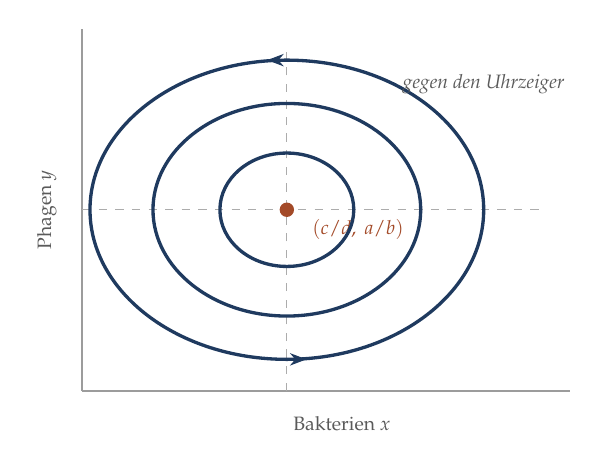
\begin{tikzpicture}[scale=1.0]
\draw[grau!60, line width=0.7pt] (0,0) -- (6.2,0);
\draw[grau!60, line width=0.7pt] (0,0) -- (0,4.6);
\draw[grau!50, dashed] (2.6,0) -- (2.6,4.3);
\draw[grau!50, dashed] (0,2.3) -- (5.9,2.3);
\fill[akzent] (2.6,2.3) circle (2.6pt);
\node[font=\scriptsize, color=akzent, anchor=west] at (2.8,2.05) {$(c/d,\ a/b)$};
\draw[tief, line width=1.2pt] (2.6,2.3) ellipse (0.85 and 0.72);
\draw[tief, line width=1.2pt] (2.6,2.3) ellipse (1.7 and 1.35);
\draw[tief, line width=1.2pt] (2.6,2.3) ellipse (2.5 and 1.9);
\draw[tief, -{Stealth[length=6pt]}] (2.6,4.2) -- (2.35,4.2);
\draw[tief, -{Stealth[length=6pt]}] (2.6,0.4) -- (2.85,0.4);
\node[font=\scriptsize, color=grau] at (3.3,-0.42) {Bakterien $x$};
\node[font=\scriptsize, color=grau, rotate=90] at (-0.45,2.3) {Phagen $y$};
\node[font=\scriptsize\itshape, color=grau] at (5.1,3.9) {gegen den Uhrzeiger};
\end{tikzpicture}
\end{center}

\schritt{Die vier Viertel}
\begin{center}
{\small
\renewcommand{\arraystretch}{1.5}
\begin{tabular}{@{}P{2.6cm}P{2.4cm}P{3.0cm}@{}}
\toprule
\textbf{Lage} & \textbf{Bakterien} & \textbf{Phagen}\\
\midrule
wenig von beidem & \textcolor{gruen}{wachsen} & \textcolor{akzent}{sterben}\\
viele Bakterien, wenige Phagen & \textcolor{gruen}{wachsen} & \textcolor{gruen}{wachsen}\\
viele von beidem & \textcolor{akzent}{sterben} & \textcolor{gruen}{wachsen}\\
wenige Bakterien, viele Phagen & \textcolor{akzent}{sterben} & \textcolor{akzent}{sterben}\\
\bottomrule
\end{tabular}}
\end{center}

\begin{center}
\begin{minipage}{0.88\textwidth}
\kursiv{Diese Reihenfolge erzeugt die Umlaufbewegung: Auf viele Bakterien folgen viele Phagen, auf viele Phagen wenige Bakterien, auf wenige Bakterien wenige Phagen --- und dann beginnt es von vorn. Der Räuber folgt der Beute mit einer Verzögerung von etwa einem Viertel Umlauf.}
\end{minipage}
\end{center}
\end{merksatz}

\begin{merksatz}
\boxtitel{Satz 4.3 --- eine Erhaltungsgröße}
Entlang jeder Bahn ist die Größe
\[ V(x,y) \;=\; d\,x - c\,\ln x + b\,y - a\,\ln y \]
konstant.

\schritt{Beweis}
Wir leiten $V$ nach der Zeit ab. Nach der Kettenregel:
\[ \frac{\dd V}{\dd t} = \left(d - \frac{c}{x}\right)\frac{\dd x}{\dd t} + \left(b - \frac{a}{y}\right)\frac{\dd y}{\dd t} \]

Die Ableitungen einsetzen:
\[ = \left(d - \frac{c}{x}\right)x(a-by) + \left(b - \frac{a}{y}\right)y(-c+dx) \]

Ausmultiplizieren --- $x$ beziehungsweise $y$ hineinziehen:
\[ = (dx - c)(a-by) + (by - a)(-c+dx) \]

Im zweiten Summanden klammern wir $-1$ zweimal aus:
\[ (by-a)(-c+dx) = -(a-by)\cdot(dx-c) \]

Also
\[ \frac{\dd V}{\dd t} = (dx-c)(a-by) - (a-by)(dx-c) = 0 . \qquad \blacksquare \]
\end{merksatz}

\begin{merksatz}
\boxtitel{Was das bedeutet}
\begin{center}
\begin{minipage}{0.9\textwidth}
\textbf{Jede Bahn ist eine geschlossene Kurve.} Das System kehrt immer wieder exakt zu seinem Ausgangszustand zurück --- und zwar für jeden Startwert.
\end{minipage}
\end{center}

\schritt{Woher die geschlossenen Bahnen kommen}
Die Bahn liegt auf einer Höhenlinie von $V$. Man kann zeigen, dass $V$ genau ein Minimum hat --- im Gleichgewichtspunkt --- und nach außen überall wächst. Die Höhenlinien einer solchen Funktion sind geschlossene Kurven um das Minimum.

\schritt{Die Periode nahe am Gleichgewicht}
Für kleine Auslenkungen ergibt die Linearisierung eine Schwingung mit der Kreisfrequenz $\sqrt{ac}$, also der Periode
\[ T = \frac{2\pi}{\sqrt{ac}} . \]

\kursiv{Für die Phagen am Klinikum:}
\[ T = \frac{2\pi}{\sqrt{1{,}0 \cdot 0{,}4}} = \frac{6{,}283}{0{,}6325} = 9{,}93\ \text{Stunden} . \]

\begin{center}
\begin{minipage}{0.88\textwidth}
\kursiv{Bemerkenswert: Die Periode hängt nur von $a$ und $c$ ab --- den Raten, mit denen jede Art \kursiv{allein} wächst oder stirbt. Die Wechselwirkungsstärken $b$ und $d$ bestimmen, wo das Gleichgewicht liegt, aber nicht, wie schnell umgelaufen wird.}
\end{minipage}
\end{center}
\end{merksatz}

\section{Volterras Prinzip}

Jetzt das Ergebnis, um dessentwillen dieses Kapitel geschrieben ist.

\begin{merksatz}
\boxtitel{Satz 4.4 --- die Mittelwerte über eine Periode}
Sei $T$ die Umlaufdauer einer Bahn. Dann gilt für die zeitlichen Mittelwerte
\[ \overline{x} = \frac{1}{T}\int_0^T x\,\dd t = \frac{c}{d}, \qquad \overline{y} = \frac{1}{T}\int_0^T y\,\dd t = \frac{a}{b} . \]

\begin{center}
\begin{minipage}{0.9\textwidth}
\textbf{Die Mittelwerte sind genau die Gleichgewichtswerte --- und zwar für \kursiv{jede} Bahn, gleichgültig wie groß die Schwingung ist.}
\end{minipage}
\end{center}
\end{merksatz}

\begin{merksatz}
\boxtitel{Beweis --- kurz und überraschend}
\schritt{Schritt 1 --- Die Gleichung umschreiben}
Wir teilen die erste Gleichung durch $x$:
\[ \frac{1}{x}\frac{\dd x}{\dd t} = a - b\,y \]

Links steht nach der Kettenregel gerade die Ableitung des Logarithmus:
\[ \frac{\dd}{\dd t}\ln x(t) = \frac{1}{x}\frac{\dd x}{\dd t} \]

Also
\[ \frac{\dd}{\dd t}\ln x = a - b\,y . \]

\schritt{Schritt 2 --- Über eine Periode integrieren}
\[ \int_0^T \frac{\dd}{\dd t}\ln x\,\dd t = \int_0^T (a - by)\,\dd t \]

Links steht nach dem Hauptsatz der Differential- und Integralrechnung
\[ \ln x(T) - \ln x(0) . \]

\schritt{Schritt 3 --- Der entscheidende Punkt}
Die Bahn ist geschlossen, also $x(T) = x(0)$. Damit ist die linke Seite \textbf{null}.

\schritt{Schritt 4 --- Auflösen}
\[ 0 = \int_0^T a\,\dd t - b\int_0^T y\,\dd t = aT - b\int_0^T y\,\dd t \]
\[ \int_0^T y\,\dd t = \frac{aT}{b} \quad\Longrightarrow\quad \overline y = \frac{1}{T}\cdot\frac{aT}{b} = \frac{a}{b} \]

\schritt{Schritt 5 --- Dasselbe für $x$}
Aus der zweiten Gleichung, durch $y$ geteilt:
\[ \frac{\dd}{\dd t}\ln y = -c + d\,x \]
Integrieren über eine Periode ergibt $0 = -cT + d\int_0^T x\,\dd t$, also $\overline x = c/d$. $\blacksquare$

\begin{center}
\begin{minipage}{0.88\textwidth}
\kursiv{Der Beweis benutzt keine einzige Eigenschaft der Bahn außer ihrer Geschlossenheit. Deshalb gilt er für alle Schwingungsgrößen gleichermaßen --- man muss die Bahn nicht kennen, nicht ausrechnen und nicht einmal wissen, wie lange $T$ ist.}
\end{minipage}
\end{center}
\end{merksatz}

\begin{merksatz}
\boxtitel{Die Folgerung: Volterras Prinzip}
Wir bekämpfen nun \kursiv{beide} Arten gleichzeitig --- etwa mit einem Mittel, das Bakterien und Phagen gleichermaßen abtötet, mit der Rate $h$:
\[ \frac{\dd x}{\dd t} = x\,(a - h - b\,y), \qquad \frac{\dd y}{\dd t} = y\,(-c - h + d\,x) \]

\schritt{Die neuen Mittelwerte}
Dieselbe Rechnung, mit $a \to a-h$ und $c \to c+h$:
\[ \overline{x} = \frac{c+h}{d}, \qquad \overline{y} = \frac{a-h}{b} \]

\begin{center}
\begin{minipage}{0.9\textwidth}
\textbf{Die Bekämpfung erhöht den mittleren Bestand der Beute und senkt den der Räuber.}
\end{minipage}
\end{center}

\schritt{Am Zahlenbeispiel}
\begin{center}
\renewcommand{\arraystretch}{1.48}
\begin{tabular}{@{}P{2.2cm}P{2.2cm}P{2.2cm}@{}}
\toprule
$h$ & $\overline x$ (Bakterien) & $\overline y$ (Phagen)\\
\midrule
$0$ & $2{,}00$ & $2{,}00$\\
$0{,}2$ & $3{,}00$ & $1{,}60$\\
$0{,}4$ & $4{,}00$ & $1{,}20$\\
$0{,}6$ & $5{,}00$ & $0{,}80$\\
$1{,}0$ & $7{,}00$ & \textcolor{akzent}{$0{,}00$}\\
\bottomrule
\end{tabular}
\end{center}

\kursiv{Rechnung für $h=0{,}4$:} $\overline x = (0{,}4+0{,}4)/0{,}2 = 4{,}0$ und $\overline y = (1{,}0-0{,}4)/0{,}5 = 1{,}2$.

\begin{center}
\begin{minipage}{0.9\textwidth}
\textbf{Ein Mittel, das beide tötet, verdoppelt den mittleren Bakterienbestand.} Bei $h \ge a$ verschwinden die Phagen ganz, und die Bakterien wachsen wieder unbeschränkt.
\end{minipage}
\end{center}
\end{merksatz}

\begin{warnung}
\boxtitelr{Warum das folgenreich ist}
Der Befund erklärt eine Beobachtung, die zunächst unverständlich schien.

\schritt{Die Adria, 1914 bis 1923}
Der Zoologe Umberto D'Ancona untersuchte die Fangstatistiken der Adriahäfen. Er fand, dass während des Ersten Weltkriegs --- als kaum gefischt wurde --- der Anteil der \kursiv{Raubfische} am Fang deutlich \textbf{stieg}.

\begin{center}
\begin{minipage}{0.9\textwidth}
Weniger Fischerei führte zu mehr Räubern, nicht zu mehr Beutefischen. D'Ancona konnte sich das nicht erklären und wandte sich an seinen Schwiegervater Vito Volterra.
\end{minipage}
\end{center}

\schritt{Die Auflösung}
Genau das sagt Satz 4.4 vorher. Fischerei wirkt wie das Mittel mit Rate $h$: Sie trifft beide Arten. Verringert man $h$, so steigt $\overline y$ und sinkt $\overline x$.

\schritt{Die allgemeine Regel}
\begin{center}
\begin{minipage}{0.9\textwidth}
\textbf{Wer in ein Räuber-Beute-System eingreift und beide Arten gleichermaßen trifft, begünstigt die Beute.}
\end{minipage}
\end{center}

\schritt{Wo das heute eine Rolle spielt}
\begin{center}
{\small
\renewcommand{\arraystretch}{1.5}
\begin{tabular}{@{}P{2.6cm}P{6.0cm}@{}}
\toprule
\textbf{Schädlings\-bekämpfung} & Ein Breitbandmittel tötet Schädling und Nützling. Der Schädling kann danach häufiger sein als vorher.\\
\textbf{Antibiotika} & Ein Breitbandantibiotikum trifft auch die konkurrierende Normalflora --- Kapitel~5.\\
\textbf{Fischerei} & Der ursprüngliche Fall; heute Grundlage von Fangquotenmodellen.\\
\bottomrule
\end{tabular}}
\end{center}

\begin{center}
\begin{minipage}{0.88\textwidth}
\kursiv{Die erste Zeile ist in der Landwirtschaft gut belegt: Nach Breitbandbehandlungen treten regelmäßig Schädlingsvermehrungen auf, die stärker sind als vor dem Eingriff. Man nennt das \Begriff{Sekundärgradation}, und Volterras Prinzip ist ihre einfachste Erklärung.}
\end{minipage}
\end{center}
\end{warnung}

\section{Der Bruchfall}

\begin{warnung}
\boxtitelr{Das Modell ist strukturell instabil}
Die geschlossenen Bahnen sind eine sehr besondere Eigenschaft. Sie verschwinden bei der kleinsten Änderung des Modells.

\schritt{Ein Beispiel}
Gibt man der Beute eine Kapazitätsgrenze --- wie in Kapitel~2 ---, so lautet die erste Gleichung
\[ \frac{\dd x}{\dd t} = x\left(a\left(1-\frac{x}{K}\right) - b\,y\right) . \]

Die Bahnen sind dann keine geschlossenen Kurven mehr, sondern Spiralen, die auf das Gleichgewicht zulaufen. Die Schwingungen klingen ab.

\begin{center}
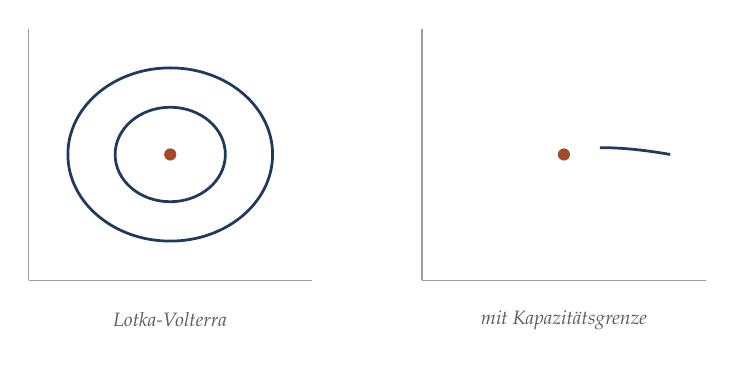
\begin{tikzpicture}[scale=1.0]
\begin{scope}
\draw[grau!60, line width=0.6pt] (0,0) -- (3.6,0);
\draw[grau!60, line width=0.6pt] (0,0) -- (0,3.2);
\fill[akzent] (1.8,1.6) circle (2.2pt);
\draw[tief, line width=1.0pt] (1.8,1.6) ellipse (1.3 and 1.1);
\draw[tief, line width=1.0pt] (1.8,1.6) ellipse (0.7 and 0.6);
\node[font=\scriptsize\itshape, color=grau] at (1.8,-0.5) {Lotka-Volterra};
\end{scope}
\begin{scope}[xshift=5.0cm]
\draw[grau!60, line width=0.6pt] (0,0) -- (3.6,0);
\draw[grau!60, line width=0.6pt] (0,0) -- (0,3.2);
\fill[akzent] (1.8,1.6) circle (2.2pt);
\draw[tief, line width=1.0pt, smooth, samples=100, domain=0:12.5]
  plot ({1.8+1.35*exp(-0.085*\x)*cos(\x)}, {1.6+1.15*exp(-0.085*\x)*sin(\x)});
\node[font=\scriptsize\itshape, color=grau] at (1.8,-0.5) {mit Kapazitätsgrenze};
\end{scope}
\end{tikzpicture}
\end{center}

\schritt{Warum das ein Mangel ist}
\begin{center}
\begin{minipage}{0.9\textwidth}
Ein Modell, dessen wichtigste Eigenschaft bei jeder kleinen Änderung verschwindet, beschreibt nichts Robustes. Die Natur enthält immer solche kleinen Änderungen.
\end{minipage}
\end{center}

\begin{center}
\begin{minipage}{0.88\textwidth}
\kursiv{Man sagt, das Modell sei \Begriff{strukturell instabil}. Die geschlossenen Bahnen sind ein Artefakt der besonderen Bauweise, nicht eine Vorhersage. Beobachtete Populationszyklen --- etwa die bekannten Schwankungen von Schneeschuhhase und Luchs --- sind daher \kursiv{nicht} als Beleg für dieses Modell zu lesen.}
\end{minipage}
\end{center}

\schritt{Was trotzdem bleibt}
\begin{center}
\renewcommand{\arraystretch}{1.5}
\begin{tabular}{@{}P{3.0cm}P{5.6cm}@{}}
\toprule
\textbf{Gleich\-gewichtslage} & Die Überkreuz-Beziehung bleibt auch in verfeinerten Modellen erhalten.\\
\textbf{Volterras Prinzip} & Gilt ebenfalls allgemeiner --- die Richtung des Effekts bleibt.\\
\textbf{Die Verzögerung} & Der Räuber folgt der Beute --- das ist ein robustes Merkmal.\\
\bottomrule
\end{tabular}
\end{center}
\end{warnung}

\begin{warnung}
\boxtitelr{Und eine Unstimmigkeit, die auffallen sollte}
Bei kleinem $x$ und kleinem $y$ wächst die Beute exponentiell. Das Modell kennt also weder eine Obergrenze noch ein Aussterben durch Zufall.

\begin{center}
\begin{minipage}{0.88\textwidth}
\kursiv{Läuft eine Bahn sehr nahe an die Achsen heran --- was bei großen Schwingungen geschieht ---, so sinkt der Bestand auf Werte wie $0{,}001$ Einheiten. Bei $10^6$ je Einheit wären das noch tausend Zellen; bei einer Tierpopulation wären es weniger als ein Individuum. Ein stetiges Modell rechnet das ohne Bedenken weiter. In Wirklichkeit ist die Art dann ausgestorben.}
\end{minipage}
\end{center}

\begin{center}
\begin{minipage}{0.9\textwidth}
\textbf{Stetige Modelle kennen keine ganzen Zahlen und kein Aussterben.} Bei kleinen Beständen muss man zu stochastischen Modellen übergehen.
\end{minipage}
\end{center}
\end{warnung}

\section{Übungsaufgaben}

\begin{aufgabe}
\boxtitel{Aufgabe 4.1 --- Gleichgewicht und Periode}
Für ein Räuber-Beute-System gilt $a = 0{,}8\ \mathrm{d}^{-1}$, $b = 0{,}004$, $c = 0{,}5\ \mathrm{d}^{-1}$, $d = 0{,}001$. Bestimmen Sie das Gleichgewicht, die Periode kleiner Schwingungen und deuten Sie das Ergebnis.

\loesung
\schritt{Schritt 1 --- Das Gleichgewicht}
\[ x^{*} = \frac{c}{d} = \frac{0{,}5}{0{,}001} = 500 \ \text{Beutetiere} \]
\[ y^{*} = \frac{a}{b} = \frac{0{,}8}{0{,}004} = 200 \ \text{Räuber} \]

\schritt{Schritt 2 --- Die Periode}
\[ T = \frac{2\pi}{\sqrt{ac}} = \frac{6{,}283}{\sqrt{0{,}8 \cdot 0{,}5}} = \frac{6{,}283}{\sqrt{0{,}4}} = \frac{6{,}283}{0{,}6325} = 9{,}93\ \text{Tage} \]

\schritt{Schritt 3 --- Die Probe über die Einheiten}
$a$ und $c$ haben die Einheit $\mathrm{d}^{-1}$, also hat $\sqrt{ac}$ ebenfalls $\mathrm{d}^{-1}$, und $T$ hat die Einheit Tage. \checkmark

\schritt{Schritt 4 --- Was geschieht, wenn die Beute schneller wächst?}
Verdoppeln wir $a$ auf $1{,}6$:
\begin{center}
\renewcommand{\arraystretch}{1.48}
\begin{tabular}{@{}P{2.4cm}P{2.0cm}P{2.0cm}P{1.8cm}@{}}
\toprule
& $x^{*}$ & $y^{*}$ & $T$\\
\midrule
$a = 0{,}8$ & $500$ & $200$ & $9{,}93$ d\\
$a = 1{,}6$ & $\mathbf{500}$ & $\mathbf{400}$ & $7{,}02$ d\\
\bottomrule
\end{tabular}
\end{center}

\begin{center}
\begin{minipage}{0.88\textwidth}
\kursiv{Der Beutebestand bleibt unverändert bei $500$; die Räuber verdoppeln sich. Das ist die Überkreuz-Eigenschaft aus Abschnitt 4.2, in Zahlen. Wer die Beute fördert --- etwa durch besseres Futterangebot --- fördert die Räuber.}
\end{minipage}
\end{center}

\schritt{Schritt 5 --- Und wenn man die Räuber dezimiert?}
Verdoppeln wir $c$ auf $1{,}0$ --- die Räuber sterben doppelt so schnell:
\[ x^{*} = \frac{1{,}0}{0{,}001} = 1000, \qquad y^{*} = 200 \ \text{unverändert} . \]

Die Beute verdoppelt sich, die Räuber bleiben gleich.

\begin{center}
\begin{minipage}{0.86\textwidth}
\kursiv{Auch das ist überkreuz --- und es ist die Gegenprobe zu Volterras Prinzip: Trifft man \kursiv{nur} die Räuber, so nützt das der Beute, ohne den Räubern im Mittel zu schaden. Die Kunst liegt in der Auswahl.}
\end{minipage}
\end{center}
\end{aufgabe}

\begin{aufgabe}
\boxtitel{Aufgabe 4.2 --- Schädlingsbekämpfung durchrechnen}
Ein Schädling ($x$) wird von einem Nützling ($y$) kurzgehalten: $a = 2{,}0$, $b = 0{,}01$, $c = 0{,}8$, $d = 0{,}004$ (je Woche). Ein Breitbandmittel tötet beide mit der Rate $h$. Wie ändern sich die Mittelwerte?

\loesung
\schritt{Schritt 1 --- Ohne Behandlung}
\[ \overline x = \frac{c}{d} = \frac{0{,}8}{0{,}004} = 200, \qquad \overline y = \frac{a}{b} = \frac{2{,}0}{0{,}01} = 200 \]

\schritt{Schritt 2 --- Mit Behandlung}
\[ \overline x = \frac{c+h}{d} = \frac{0{,}8+h}{0{,}004}, \qquad \overline y = \frac{a-h}{b} = \frac{2{,}0-h}{0{,}01} \]

\begin{center}
{\small
\renewcommand{\arraystretch}{1.48}
\begin{tabular}{@{}P{1.6cm}P{2.2cm}P{2.2cm}P{2.0cm}@{}}
\toprule
$h$ & $\overline x$ (Schädling) & $\overline y$ (Nützling) & \textbf{Änderung}\\
\midrule
$0$ & $200$ & $200$ & ---\\
$0{,}4$ & $300$ & $160$ & $+50\,\%$\\
$0{,}8$ & $400$ & $120$ & $+100\,\%$\\
$1{,}2$ & $500$ & $80$ & $+150\,\%$\\
$2{,}0$ & $700$ & \textcolor{akzent}{$0$} & \textcolor{akzent}{Nützling weg}\\
\bottomrule
\end{tabular}}
\end{center}

\schritt{Schritt 3 --- Die Deutung}
\begin{center}
\begin{minipage}{0.9\textwidth}
\textbf{Je stärker behandelt wird, desto größer der mittlere Schädlingsbestand.} Bei $h = 2{,}0$ ist der Nützling ausgerottet, und der Schädling wächst danach unbegrenzt.
\end{minipage}
\end{center}

\schritt{Schritt 4 --- Der scheinbare Widerspruch zur Erfahrung}
Nach einer Behandlung beobachtet man zunächst sehr wohl einen Rückgang. Das Modell widerspricht dem nicht --- es macht eine Aussage über den \kursiv{Mittelwert über eine Periode}, nicht über den Verlauf unmittelbar danach.

\begin{center}
\begin{minipage}{0.88\textwidth}
\kursiv{Genau darin liegt die Tücke: Der kurzfristige Erfolg ist sichtbar, der langfristige Schaden nicht. Wer nach jeder Behandlung den sofortigen Rückgang misst, wird das Mittel für wirksam halten --- und häufiger behandeln müssen als vorher.}
\end{minipage}
\end{center}

\schritt{Schritt 5 --- Was stattdessen hilft}
Ein Mittel, das \kursiv{nur} den Schädling trifft, wirkt wie eine Erhöhung von $c$ --- nein, genauer: Es erhöht die Sterberate der Beute, verändert also $a$ zu $a - h$, ohne $c$ zu berühren:
\[ \overline x = \frac{c}{d} = 200 \ \text{unverändert}, \qquad \overline y = \frac{a-h}{b} \ \text{sinkt} . \]

\begin{center}
\begin{minipage}{0.88\textwidth}
\kursiv{Also nützt auch das nichts --- im Mittel! Der Schädlingsbestand bleibt bei $200$, und man schadet dem Nützling. Die einzige Maßnahme, die den mittleren Schädlingsbestand senkt, ist eine, die den \kursiv{Nützling fördert}: Eine Verringerung von $c$ oder eine Erhöhung von $d$ senkt $\overline x = c/d$.}
\end{minipage}
\end{center}

\begin{center}
\begin{minipage}{0.9\textwidth}
\textbf{Das ist die Grundlage der biologischen Schädlingsbekämpfung} --- und sie folgt unmittelbar aus der Überkreuz-Eigenschaft.
\end{minipage}
\end{center}
\end{aufgabe}

\begin{aufgabe}
\boxtitel{Aufgabe 4.3 --- Die Erhaltungsgröße nutzen}
Für $a = 1{,}0$, $b = 0{,}5$, $c = 0{,}4$, $d = 0{,}2$ startet das System bei $x_0 = 4{,}0$ und $y_0 = 2{,}0$. Bestimmen Sie den Wert der Erhaltungsgröße und daraus den kleinsten vorkommenden Bakterienbestand.

\loesung
\schritt{Schritt 1 --- Die Erhaltungsgröße am Startpunkt}
\[ V = d\,x - c\ln x + b\,y - a\ln y \]
\[ V_0 = 0{,}2 \cdot 4 - 0{,}4\ln 4 + 0{,}5 \cdot 2 - 1{,}0\ln 2 \]
\[ = 0{,}8 - 0{,}4 \cdot 1{,}3863 + 1{,}0 - 0{,}6931 \]
\[ = 0{,}8 - 0{,}5545 + 1{,}0 - 0{,}6931 = 0{,}5524 \]

\schritt{Schritt 2 --- Wo der kleinste $x$-Wert liegt}
Auf einer geschlossenen Bahn wird $x$ dort am kleinsten, wo die Bahn senkrecht verläuft --- also wo $\dd x/\dd t = 0$ bei $\dd y/\dd t \neq 0$. Aus $x(a-by) = 0$ und $x > 0$:
\[ y = \frac{a}{b} = \frac{1{,}0}{0{,}5} = 2{,}0 = y^{*} \]

\begin{center}
\begin{minipage}{0.88\textwidth}
\kursiv{Die Extremwerte von $x$ werden also stets bei $y = y^{*}$ angenommen --- und umgekehrt. Die Bahn hat ihre waagerechten und senkrechten Tangenten genau auf den beiden gestrichelten Linien des Phasenporträts.}
\end{minipage}
\end{center}

\schritt{Schritt 3 --- Die Gleichung für $x$}
Wir setzen $y = 2{,}0$ und $V = 0{,}5524$ ein:
\[ 0{,}5524 = 0{,}2x - 0{,}4\ln x + 0{,}5 \cdot 2 - 1{,}0\ln 2 \]
\[ 0{,}5524 = 0{,}2x - 0{,}4\ln x + 1{,}0 - 0{,}6931 \]
\[ 0{,}2x - 0{,}4\ln x = 0{,}5524 - 0{,}3069 = 0{,}2455 \]

\schritt{Schritt 4 --- Lösen}
Die Gleichung $0{,}2x - 0{,}4\ln x = 0{,}2455$ lässt sich nicht geschlossen auflösen. Wir probieren:

\begin{center}
\renewcommand{\arraystretch}{1.42}
\begin{tabular}{@{}P{1.6cm}P{2.2cm}P{2.4cm}@{}}
\toprule
$x$ & $0{,}2x-0{,}4\ln x$ & \\
\midrule
$4{,}0$ & $0{,}2455$ & \textcolor{gruen}{der Startwert}\\
$2{,}0$ & $0{,}1227$ & zu klein\\
$1{,}0$ & $0{,}2000$ & zu klein\\
$0{,}8$ & $0{,}2493$ & knapp zu groß\\
$0{,}82$ & $0{,}2432$ & knapp zu klein\\
$\mathbf{0{,}81}$ & $\mathbf{0{,}2462}$ & \textcolor{gruen}{nahe genug}\\
\bottomrule
\end{tabular}
\end{center}

\schritt{Antwort}
Der kleinste Bakterienbestand beträgt etwa $\mathbf{0{,}81}$ Einheiten --- also $8{,}1\cdot10^{5}$ je Milliliter.

\schritt{Schritt 5 --- Die Probe}
Der Startwert $x_0 = 4{,}0$ liefert denselben Wert des Ausdrucks. Das muss so sein: Auch der Start lag bei $y = 2{,}0 = y^{*}$, also ist $x_0$ selbst ein Extremwert --- nämlich der \kursiv{größte}.

\begin{center}
\begin{minipage}{0.88\textwidth}
\kursiv{Die Bahn schwankt also zwischen $0{,}81$ und $4{,}0$ Einheiten Bakterien --- um den Mittelwert $\overline x = c/d = 2{,}0$. Beachten Sie, dass die Schwankung \kursiv{unsymmetrisch} ist: $1{,}19$ nach unten, $2{,}0$ nach oben. Der zeitliche Mittelwert ist dennoch genau $2{,}0$, weil sich das System in den unteren Bereichen länger aufhält.}
\end{minipage}
\end{center}

\schritt{Schritt 6 --- Warum das praktisch wichtig ist}
Bei $8{,}1\cdot10^5$ Bakterien je Milliliter ist die Population noch groß. Wäre die Anfangsauslenkung stärker gewesen --- etwa $x_0 = 20$ ---, so läge das Minimum um Größenordnungen tiefer, und das Aussterben durch Zufall würde wahrscheinlich.

\begin{center}
\begin{minipage}{0.86\textwidth}
\kursiv{Das ist die praktische Bedeutung der Erhaltungsgröße: Sie sagt, wie tief die Täler werden --- und damit, ob eine Phagentherapie den Erreger tatsächlich auslöschen könnte. Kapitel~5 und 9 gehen dieser Frage nach.}
\end{minipage}
\end{center}
\end{aufgabe}

\begin{geschichte}
\boxtitelg{Ein Schwiegervater, ein Versicherungsmathematiker und die Adria}
\Person{Vito Volterra} (1860--1940) war einer der führenden italienischen Mathematiker seiner Zeit --- Senator, Präsident der Accademia dei Lincei, Begründer der Funktionalanalysis.

1925 stellte ihm sein Schwiegersohn \Person{Umberto D'Ancona} die Frage aus dem Warnkasten: Warum stieg der Raubfischanteil, als weniger gefischt wurde? Volterra stellte binnen weniger Monate die Gleichungen auf und leitete das Prinzip her, das heute seinen Namen trägt.

\begin{center}
\begin{minipage}{0.9\textwidth}
\kursiv{Er war damals fünfundsechzig und hatte nie zuvor über Biologie gearbeitet. Die Arbeit von 1926 begründete ein ganzes Fach.}
\end{minipage}
\end{center}

\schritt{Der Vorläufer}
\Person{Alfred Lotka} (1880--1949), in Lemberg geborener Chemiker, der später als Versicherungsmathematiker bei einer amerikanischen Gesellschaft arbeitete, hatte dieselben Gleichungen bereits 1920 aufgestellt --- allerdings als Modell für eine chemische Reaktion, nicht für Populationen.

Als Volterras Arbeit erschien, wies Lotka in einem Brief an \kursiv{Nature} auf seine Priorität hin. Volterra räumte sie ein. Die Gleichungen tragen seither beide Namen.

\schritt{Ein Nachwort zu Volterra}
1931 verweigerte Volterra als einer von nur zwölf italienischen Professoren den Treueid auf den Faschismus. Er verlor seinen Lehrstuhl, wurde aus allen Akademien ausgeschlossen und arbeitete bis zu seinem Tod 1940 im Ausland und zu Hause weiter.

\begin{center}
\begin{minipage}{0.9\textwidth}
\kursiv{Von den etwa zwölfhundert italienischen Hochschullehrern jener Zeit verweigerten zwölf. Volterra war der bekannteste unter ihnen.}
\end{minipage}
\end{center}
\end{geschichte}

\begin{forschung}
\boxtitelp{Wie es weiterging}
\begin{center}
{\small
\renewcommand{\arraystretch}{1.45}
\begin{tabular}{@{}P{2.8cm}P{5.4cm}@{}}
\toprule
\textbf{Realistischere Funktionen} & Statt $bxy$ nimmt man eine sättigende Fraßrate --- ein Räuber kann nur begrenzt viel fressen. Das erzeugt statt geschlossener Bahnen einen \Begriff{Grenzzyklus}.\\
\textbf{Grenzzyklen} & Eine einzelne geschlossene Bahn, auf die alle anderen zulaufen. Strukturell stabil --- und damit ein brauchbares Modell für beobachtete Zyklen.\\
\textbf{Phagentherapie} & Seit etwa 2015 wieder ernsthaft untersucht, wegen zunehmender Antibiotikaresistenz. Die Modelle sind Weiterentwicklungen dieses Kapitels.\\
\bottomrule
\end{tabular}}
\end{center}

Die dritte Zeile ist der Anschluss an den Leitfall. Die entscheidende Frage lautet dort, ob Bakterien Resistenz gegen den Phagen entwickeln --- was sie tun --- und ob diese Resistenz Kosten hat, die sie gegenüber anderen Stämmen benachteiligen.

\begin{center}
\begin{minipage}{0.88\textwidth}
\kursiv{Ein besonders untersuchter Fall: Manche Bakterien werden phagenresistent, indem sie genau den Oberflächenrezeptor verlieren, über den auch bestimmte Antibiotika angreifen --- oder umgekehrt eine Resistenz gegen Antibiotika aufgeben. Man spricht von \Begriff{Kollateralsensitivität} und versucht, Phagen und Antibiotika so zu kombinieren, dass jeder Fluchtweg in eine Falle führt. Kapitel~14 kommt darauf zurück.}
\end{minipage}
\end{center}

\schritt{Der Schneeschuhhase}
Die berühmten Zyklen von Hase und Luchs aus den Fangdaten der Hudson's Bay Company --- über hundert Jahre, mit einer Periode von etwa zehn Jahren --- gelten bis heute als Lehrbuchbeispiel. Sie sind jedoch schlecht durch Lotka-Volterra erklärbar: Unter anderem geht der Luchs dem Hasen in den Daten stellenweise \kursiv{voraus}, was das Modell nicht zulässt.

\begin{center}
\begin{minipage}{0.88\textwidth}
\kursiv{Heutige Erklärungen beziehen die Pflanzennahrung der Hasen und die Fangstatistik selbst mit ein. Das Beispiel ist also weniger ein Beleg für das Modell als eine Mahnung, wie schwer der Nachweis eines Mechanismus aus Zeitreihen ist --- dasselbe Problem wie beim Chaosnachweis in Kapitel~3.}
\end{minipage}
\end{center}
\end{forschung}

\begin{merksatz}
\boxtitel{Was Sie jetzt können}
\begin{center}
\renewcommand{\arraystretch}{1.5}
\begin{tabular}{@{}P{3.0cm}P{5.6cm}@{}}
\toprule
\textbf{Definition 4.1} & aus vier Annahmen aufgestellt\\
\textbf{Satz 4.2} & Gleichgewicht überkreuz: $(c/d,\ a/b)$\\
\textbf{Satz 4.3} & eine Erhaltungsgröße, also geschlossene Bahnen\\
\textbf{Satz 4.4} & \textbf{Volterras Prinzip} --- Bekämpfung nützt der Beute\\
\textbf{Der Bruchfall} & strukturell instabil; keine ganzen Zahlen\\
\bottomrule
\end{tabular}
\end{center}

\begin{center}
\begin{minipage}{0.88\textwidth}
\kursiv{Im nächsten Kapitel wechseln wir die Beziehung: Statt Räuber und Beute betrachten wir zwei Arten, die um dasselbe konkurrieren --- und finden eine Bedingung dafür, wann beide nebeneinander bestehen können.}
\end{minipage}
\end{center}
\end{merksatz}

\chapter{Wettbewerb und Koexistenz}

\section{Zwei Stämme, ein Nährmedium}

\begin{merksatz}
\boxtitel{Der Leitfall}
Am Klinikum Neustadt treten zwei Stämme desselben Erregers auf: der ursprüngliche, \kursiv{empfindliche} Stamm $E$ und ein \kursiv{unempfindlicher} Stamm $R$.

Sie fressen dasselbe, besiedeln dieselben Nischen und behindern einander. Keiner frisst den anderen --- das unterscheidet diese Lage von Kapitel~4.

\textbf{Die Frage:} Setzt sich einer durch? Oder bestehen beide nebeneinander?
\end{merksatz}

\begin{merksatz}
\boxtitel{Die Annahme}
Wir gehen vom logistischen Modell aus (Kapitel~2) und ergänzen es um einen Punkt:

\begin{center}
\begin{minipage}{0.9\textwidth}
\textbf{Jede Art hemmt sich selbst \kursiv{und} die andere. Die Hemmung durch die andere Art wird in Einheiten der eigenen umgerechnet.}
\end{minipage}
\end{center}

\schritt{Der Umrechnungsfaktor}
Ein Individuum der Art $2$ hemmt die Art $1$ so stark wie $\alpha_{12}$ Individuen der eigenen Art. Der Hemmterm lautet daher
\[ \frac{x + \alpha_{12}\,y}{K_1} \]
statt $x/K_1$ wie in Kapitel~2.

\begin{center}
\renewcommand{\arraystretch}{1.48}
\begin{tabular}{@{}P{2.2cm}P{2.8cm}P{3.0cm}@{}}
\toprule
$\alpha_{12}$ & \textbf{Bedeutung} & \\
\midrule
$0$ & keine Hemmung & Arten sind unabhängig\\
$<1$ & schwächer als eigene & \textcolor{gruen}{günstig für Koexistenz}\\
$=1$ & genauso stark & völlig gleiche Nische\\
$>1$ & stärker als eigene & \textcolor{akzent}{Verdrängung droht}\\
\bottomrule
\end{tabular}
\end{center}
\end{merksatz}

\begin{definition}
\boxtitelm{Definition 5.1 --- das Konkurrenzmodell}
\[ \frac{\dd x}{\dd t} = r_1\,x\left(1 - \frac{x + \alpha_{12}\,y}{K_1}\right), \qquad \frac{\dd y}{\dd t} = r_2\,y\left(1 - \frac{y + \alpha_{21}\,x}{K_2}\right) \]
mit $r_i, K_i > 0$ und $\alpha_{12}, \alpha_{21} \ge 0$.
\end{definition}

\begin{merksatz}
\boxtitel{Die Sonderfälle}
\begin{center}
{\small
\renewcommand{\arraystretch}{1.5}
\begin{tabular}{@{}P{2.6cm}P{6.0cm}@{}}
\toprule
$y = 0$ & Die erste Gleichung wird zur logistischen Gleichung aus Kapitel~2. Art $1$ strebt gegen $K_1$.\\
$\alpha_{12} = \alpha_{21} = 0$ & Beide wachsen unabhängig gegen ihre eigenen Grenzen.\\
$\alpha_{12} = \alpha_{21} = 1$ & Beide Arten sind ununterscheidbar; nur die Summe zählt.\\
\bottomrule
\end{tabular}}
\end{center}

\begin{center}
\begin{minipage}{0.88\textwidth}
\kursiv{Die letzte Zeile ist der Fall vollständig überlappender Nischen. Er führt, wie sich zeigen wird, stets zur Verdrängung einer Art --- und ist die einfachste Form dessen, was man das Konkurrenzausschlussprinzip nennt.}
\end{minipage}
\end{center}
\end{merksatz}

\section{Nullklinen}

\begin{definition}
\boxtitelm{Definition 5.2 --- Nullkline}
Die \Begriff{$x$-Nullkline} ist die Menge aller Punkte der Ebene, in denen $\dd x/\dd t = 0$ gilt. Entsprechend für $y$.
\end{definition}

\begin{merksatz}
\boxtitel{Warum sie das Verhalten bestimmen}
Auf einer $x$-Nullkline ändert sich $x$ nicht --- die Bahn verläuft dort senkrecht. Zwischen den Nullklinen hat $\dd x/\dd t$ ein festes Vorzeichen.

\begin{center}
\begin{minipage}{0.9\textwidth}
\textbf{Man muss also nur wissen, wo die Nullklinen liegen und welche Vorzeichen dazwischen herrschen --- dann kennt man das Verhalten des Systems, ohne eine einzige Bahn auszurechnen.}
\end{minipage}
\end{center}

\schritt{Die Nullklinen dieses Modells}
Aus $\dd x/\dd t = 0$ folgt $x = 0$ oder
\[ x + \alpha_{12}\,y = K_1 . \]
Das ist eine Gerade mit den Achsenabschnitten
\[ x = K_1 \quad\text{und}\quad y = \frac{K_1}{\alpha_{12}} . \]

Entsprechend für $y$: die Gerade $y + \alpha_{21}x = K_2$ mit den Abschnitten
\[ y = K_2 \quad\text{und}\quad x = \frac{K_2}{\alpha_{21}} . \]

\begin{center}
\begin{minipage}{0.88\textwidth}
\kursiv{Beide Nullklinen sind Geraden. Das ganze Verhalten des Modells hängt daher nur davon ab, \kursiv{wie diese beiden Geraden zueinander liegen} --- und dafür gibt es genau vier Möglichkeiten.}
\end{minipage}
\end{center}
\end{merksatz}

\begin{merksatz}
\boxtitel{Die vier Lagen}
Wir vergleichen jeweils die Achsenabschnitte auf derselben Achse.

\begin{center}
{\small
\renewcommand{\arraystretch}{1.55}
\begin{tabular}{@{}P{0.7cm}P{2.6cm}P{2.4cm}P{2.4cm}@{}}
\toprule
& \textbf{Bedingung} & \textbf{Nullklinen} & \textbf{Ergebnis}\\
\midrule
$1$ & $K_1 > \frac{K_2}{\alpha_{21}}$ und $K_2 < \frac{K_1}{\alpha_{12}}$ & getrennt & \textbf{Art 1 gewinnt}\\
$2$ & $K_1 < \frac{K_2}{\alpha_{21}}$ und $K_2 > \frac{K_1}{\alpha_{12}}$ & getrennt & \textbf{Art 2 gewinnt}\\
$3$ & $K_1 < \frac{K_2}{\alpha_{21}}$ und $K_2 < \frac{K_1}{\alpha_{12}}$ & kreuzen sich & \textcolor{gruen}{\textbf{Koexistenz}}\\
$4$ & $K_1 > \frac{K_2}{\alpha_{21}}$ und $K_2 > \frac{K_1}{\alpha_{12}}$ & kreuzen sich & \textcolor{akzent}{\textbf{einer, je nach Start}}\\
\bottomrule
\end{tabular}}
\end{center}

\begin{center}
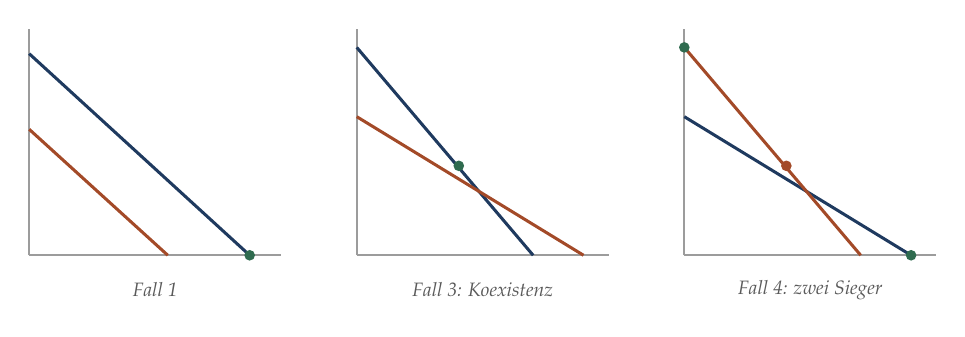
\begin{tikzpicture}[scale=0.8]
% Fall 1
\begin{scope}
\draw[grau!60, line width=0.6pt] (0,0) -- (4.0,0);
\draw[grau!60, line width=0.6pt] (0,0) -- (0,3.6);
\draw[tief, line width=1.1pt] (3.5,0) -- (0,3.2);
\draw[akzent, line width=1.1pt] (2.2,0) -- (0,2.0);
\fill[gruen] (3.5,0) circle (2.4pt);
\node[font=\scriptsize\itshape, color=grau] at (2.0,-0.55) {Fall 1};
\end{scope}
% Fall 3
\begin{scope}[xshift=5.2cm]
\draw[grau!60, line width=0.6pt] (0,0) -- (4.0,0);
\draw[grau!60, line width=0.6pt] (0,0) -- (0,3.6);
\draw[tief, line width=1.1pt] (2.8,0) -- (0,3.3);
\draw[akzent, line width=1.1pt] (3.6,0) -- (0,2.2);
\fill[gruen] (1.62,1.42) circle (2.4pt);
\node[font=\scriptsize\itshape, color=grau] at (2.0,-0.55) {Fall 3: Koexistenz};
\end{scope}
% Fall 4
\begin{scope}[xshift=10.4cm]
\draw[grau!60, line width=0.6pt] (0,0) -- (4.0,0);
\draw[grau!60, line width=0.6pt] (0,0) -- (0,3.6);
\draw[tief, line width=1.1pt] (3.6,0) -- (0,2.2);
\draw[akzent, line width=1.1pt] (2.8,0) -- (0,3.3);
\fill[akzent] (1.62,1.42) circle (2.4pt);
\fill[gruen] (3.6,0) circle (2.4pt);
\fill[gruen] (0,3.3) circle (2.4pt);
\node[font=\scriptsize\itshape, color=grau] at (2.0,-0.55) {Fall 4: zwei Sieger};
\end{scope}
\end{tikzpicture}
\end{center}

\begin{center}
\begin{minipage}{0.88\textwidth}
\kursiv{Grün markiert sind die stabilen Zustände. In Fall 4 gibt es zwei davon --- welcher erreicht wird, hängt vom Ausgangsbestand ab. Der Schnittpunkt ist dort instabil; er trennt die beiden Einzugsgebiete.}
\end{minipage}
\end{center}
\end{merksatz}

\section{Die Koexistenzbedingung}

\begin{merksatz}
\boxtitel{Satz 5.3 --- wann beide bestehen}
Die Arten können genau dann dauerhaft nebeneinander bestehen, wenn
\[ \alpha_{12} < \frac{K_1}{K_2} \qquad\text{und}\qquad \alpha_{21} < \frac{K_2}{K_1} . \]

\schritt{Beweis der ersten Bedingung}
Aus Fall 3 verlangen wir $K_2 < \frac{K_1}{\alpha_{12}}$. Umstellen --- $\alpha_{12} > 0$ und $K_2 > 0$, also darf man multiplizieren und teilen, ohne dass sich das Zeichen dreht:
\[ K_2\,\alpha_{12} < K_1 \quad\Longleftrightarrow\quad \alpha_{12} < \frac{K_1}{K_2} . \]

\schritt{Beweis der zweiten}
Entsprechend aus $K_1 < \frac{K_2}{\alpha_{21}}$:
\[ K_1\,\alpha_{21} < K_2 \quad\Longleftrightarrow\quad \alpha_{21} < \frac{K_2}{K_1} . \qquad \blacksquare \]

\schritt{Die Folgerung}
Multipliziert man beide Ungleichungen --- alle Größen sind positiv:
\[ \alpha_{12}\,\alpha_{21} < \frac{K_1}{K_2}\cdot\frac{K_2}{K_1} = 1 . \]

\begin{center}
\begin{minipage}{0.9\textwidth}
\textbf{Notwendig für Koexistenz ist $\alpha_{12}\,\alpha_{21} < 1$ --- die gegenseitige Hemmung muss im Mittel schwächer sein als die Selbsthemmung.}
\end{minipage}
\end{center}
\end{merksatz}

\begin{merksatz}
\boxtitel{Die Bedingung in Worten}
\begin{center}
\begin{minipage}{0.9\textwidth}
\textbf{Jede Art muss sich selbst stärker begrenzen als sie die andere begrenzt.}
\end{minipage}
\end{center}

\schritt{Warum das genau die richtige Bedingung ist}
Wird eine Art häufig, so hemmt sie überwiegend sich selbst. Das gibt der seltenen Art Raum, sich zu erholen.

Ist es umgekehrt --- jede hemmt die andere stärker als sich selbst ---, so verstärkt jeder Vorsprung sich selbst. Das ist Fall 4: Wer zuerst häufig ist, gewinnt.

\begin{center}
\begin{minipage}{0.88\textwidth}
\kursiv{Man nennt das Prinzip \Begriff{negative Rückkopplung auf die eigene Häufigkeit}. Es ist allgemeiner als dieses Modell und die Grundlage fast aller Koexistenzerklärungen in der Ökologie: Koexistenz braucht einen Mechanismus, der die seltene Art begünstigt.}
\end{minipage}
\end{center}
\end{merksatz}

\begin{merksatz}
\boxtitel{Satz 5.4 --- der Koexistenzpunkt}
Existiert Koexistenz, so liegt sie bei
\[ x^{*} = \frac{K_1 - \alpha_{12}K_2}{1 - \alpha_{12}\alpha_{21}}, \qquad y^{*} = \frac{K_2 - \alpha_{21}K_1}{1 - \alpha_{12}\alpha_{21}} . \]

\schritt{Beweis}
Beide Nullklinengleichungen müssen gelten:
\[ x + \alpha_{12}y = K_1 \qquad (\mathrm{I}) \]
\[ \alpha_{21}x + y = K_2 \qquad (\mathrm{II}) \]

Wir lösen $(\mathrm{II})$ nach $y$ auf: $y = K_2 - \alpha_{21}x$, und setzen in $(\mathrm{I})$ ein:
\begin{align*}
x + \alpha_{12}\bigl(K_2 - \alpha_{21}x\bigr) &= K_1\\
x + \alpha_{12}K_2 - \alpha_{12}\alpha_{21}x &= K_1\\
x\bigl(1 - \alpha_{12}\alpha_{21}\bigr) &= K_1 - \alpha_{12}K_2\\
x^{*} &= \frac{K_1 - \alpha_{12}K_2}{1 - \alpha_{12}\alpha_{21}}
\end{align*}
Einsetzen in $(\mathrm{II})$ liefert $y^{*}$. $\blacksquare$

\schritt{Die Probe an den Vorzeichen}
Unter der Koexistenzbedingung ist $\alpha_{12}K_2 < K_1$, also ist der Zähler positiv; und $\alpha_{12}\alpha_{21} < 1$, also ist der Nenner positiv. Beide Werte sind positiv. \checkmark
\end{merksatz}

\section{Der Leitfall}

\begin{merksatz}
\boxtitel{Empfindlicher und unempfindlicher Stamm --- ohne Antibiotikum}
Gemessen am Klinikum, Bestände in Einheiten von $10^8$ je Milliliter:

\begin{center}
\renewcommand{\arraystretch}{1.48}
\begin{tabular}{@{}P{2.0cm}P{1.6cm}P{4.4cm}@{}}
\toprule
$K_E$ & $10{,}0$ & Kapazität des empfindlichen Stamms\\
$K_R$ & $8{,}0$ & niedriger --- die Resistenz kostet\\
$\alpha_{ER}$ & $0{,}8$ & Hemmung von $E$ durch $R$\\
$\alpha_{RE}$ & $1{,}2$ & Hemmung von $R$ durch $E$\\
\bottomrule
\end{tabular}
\end{center}

\schritt{Die Bedingungen prüfen}
\[ \alpha_{ER} = 0{,}8 \quad\text{gegen}\quad \frac{K_E}{K_R} = \frac{10}{8} = 1{,}25 \quad\Longrightarrow\quad 0{,}8 < 1{,}25 \ \checkmark \]
\[ \alpha_{RE} = 1{,}2 \quad\text{gegen}\quad \frac{K_R}{K_E} = \frac{8}{10} = 0{,}8 \quad\Longrightarrow\quad 1{,}2 > 0{,}8 \ \textcolor{akzent}{\times} \]

Die zweite Bedingung ist verletzt: \textbf{Keine Koexistenz.}

\schritt{Wer gewinnt}
Wir bestimmen die Lage nach der Tabelle in Abschnitt 5.2:
\[ K_E = 10 \quad\text{gegen}\quad \frac{K_R}{\alpha_{RE}} = \frac{8}{1{,}2} = 6{,}67 \quad\Longrightarrow\quad 10 > 6{,}67 \]
\[ K_R = 8 \quad\text{gegen}\quad \frac{K_E}{\alpha_{ER}} = \frac{10}{0{,}8} = 12{,}5 \quad\Longrightarrow\quad 8 < 12{,}5 \]

Das ist Fall 1: \textbf{Der empfindliche Stamm verdrängt den unempfindlichen} --- und zwar von jedem Ausgangsbestand aus.

\begin{center}
\begin{minipage}{0.88\textwidth}
\kursiv{Das bestätigt die Rechnung aus Aufgabe 1.3 mit anderen Mitteln: Ohne Antibiotikum ist Resistenz ein Nachteil. Hier kommt der Grund hinzu --- $E$ ist nicht nur schneller, sondern auch der stärkere Konkurrent um dieselben Nährstoffe.}
\end{minipage}
\end{center}
\end{merksatz}

\begin{merksatz}
\boxtitel{Unter Antibiotikum}
Das Antibiotikum senkt die Kapazität des empfindlichen Stamms drastisch --- sagen wir auf $K_E = 1{,}0$.

\schritt{Neu prüfen}
\[ K_E = 1{,}0 \quad\text{gegen}\quad \frac{K_R}{\alpha_{RE}} = 6{,}67 \quad\Longrightarrow\quad 1{,}0 < 6{,}67 \]
\[ K_R = 8 \quad\text{gegen}\quad \frac{K_E}{\alpha_{ER}} = \frac{1{,}0}{0{,}8} = 1{,}25 \quad\Longrightarrow\quad 8 > 1{,}25 \]

Das ist Fall 2: \textbf{Der unempfindliche Stamm verdrängt den empfindlichen.}

\schritt{Die Umkehrung in einer Tabelle}
\begin{center}
\renewcommand{\arraystretch}{1.48}
\begin{tabular}{@{}P{2.8cm}P{2.4cm}P{2.4cm}@{}}
\toprule
& \textbf{ohne} & \textbf{mit}\\
\midrule
$K_E$ & $10{,}0$ & $1{,}0$\\
Fall & $1$ & $2$\\
Sieger & $E$ & \textcolor{akzent}{$R$}\\
Endzustand & $E = 10$, $R = 0$ & $E = 0$, $R = 8$\\
\bottomrule
\end{tabular}
\end{center}

\begin{center}
\begin{minipage}{0.88\textwidth}
\kursiv{Die Behandlung kehrt das Verhältnis vollständig um. Bemerkenswert ist, wie wenig dazu nötig war: Es genügte, \kursiv{einen} Parameter zu ändern. Alle Wechselwirkungsstärken blieben unberührt.}
\end{minipage}
\end{center}
\end{merksatz}

\begin{warnung}
\boxtitelr{Was daraus für die Behandlungsstrategie folgt}
Das Modell legt nahe, dass der empfindliche Stamm eine \kursiv{nützliche} Rolle spielt: Solange er vorhanden ist, hält er den resistenten klein.

\begin{center}
\begin{minipage}{0.9\textwidth}
\textbf{Wer den empfindlichen Stamm vollständig ausrottet, entfernt den natürlichen Konkurrenten des resistenten.}
\end{minipage}
\end{center}

\schritt{Der Gedanke der adaptiven Therapie}
Daraus ist ein Behandlungsansatz entstanden, der nicht auf vollständige Vernichtung zielt, sondern auf Eindämmung: Man behandelt nur so stark, dass die Gesamtlast beherrschbar bleibt --- und erhält dabei genug empfindliche Erreger, um den resistenten Stamm zu unterdrücken.

\begin{center}
\begin{minipage}{0.88\textwidth}
\kursiv{In der Krebsbehandlung wird dieser Ansatz seit etwa 2016 in Studien geprüft; Kapitel~14 stellt ihn ausführlich dar. In der Infektiologie ist er umstritten, weil dort eine anhaltende Erregerlast eigene Gefahren birgt --- und weil der Vergleich hinkt: Ein Tumor bleibt im Körper, ein Erreger wird weitergegeben.}
\end{minipage}
\end{center}

\schritt{Die Grenze des Arguments}
Das Modell kennt nur zwei Stämme in einem geschlossenen Gefäß. Es kennt keine Neuinfektion von außen, keine Übertragung auf andere Menschen und keine Mutation. Es begründet daher keine Behandlungsempfehlung, sondern schärft eine Frage.
\end{warnung}

\section{Der Bruchfall}

\begin{warnung}
\boxtitelr{Was dieses Modell nicht kann}
\begin{center}
{\small
\renewcommand{\arraystretch}{1.52}
\begin{tabular}{@{}P{2.8cm}P{5.8cm}@{}}
\toprule
\textbf{Feste $\alpha$} & Die Wechselwirkungsstärke gilt als Konstante. In Wirklichkeit hängt sie von den Bedingungen ab --- und vom Nährstoff, um den gerade konkurriert wird.\\
\textbf{Nur zwei Arten} & Bei drei und mehr Arten treten Erscheinungen auf, die im Zweiartenmodell unmöglich sind --- etwa zyklische Überlegenheit.\\
\textbf{Kein Raum} & Alles ist durchmischt. Räumliche Trennung ermöglicht Koexistenz auch dort, wo das Modell sie ausschließt.\\
\textbf{Keine Schwankung} & Wechselnde Bedingungen können Arten abwechselnd begünstigen und so Koexistenz erzeugen.\\
\bottomrule
\end{tabular}}
\end{center}

\schritt{Zur zweiten Zeile}
Bei drei Arten kann $A$ über $B$ siegen, $B$ über $C$ und $C$ über $A$ --- wie bei Schere, Stein, Papier. Alle drei bestehen dann dauerhaft nebeneinander, obwohl je zwei von ihnen es nicht könnten.

\begin{center}
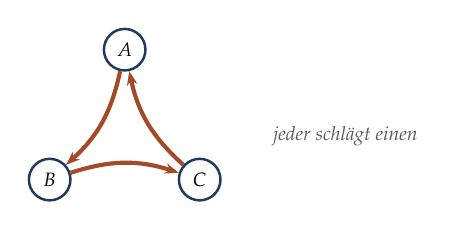
\begin{tikzpicture}[scale=1.1]
\node[knotenb] (a) at (90:1.0) {$A$};
\node[knotenb] (b) at (210:1.0) {$B$};
\node[knotenb] (c) at (330:1.0) {$C$};
\draw[kanted, -{Stealth[length=5pt]}] (a) to[bend left=18] (b);
\draw[kanted, -{Stealth[length=5pt]}] (b) to[bend left=18] (c);
\draw[kanted, -{Stealth[length=5pt]}] (c) to[bend left=18] (a);
\node[font=\scriptsize\itshape, color=grau, anchor=west] at (1.6,0) {jeder schlägt einen};
\end{tikzpicture}
\end{center}

\begin{center}
\begin{minipage}{0.88\textwidth}
\kursiv{Bei Darmbakterien ist das beobachtet: Manche Stämme erzeugen Giftstoffe gegen andere, sind aber selbst gegen einen dritten empfindlich. Solche Dreiecksbeziehungen gelten heute als eine Erklärung dafür, wie in der Darmflora Hunderte von Arten nebeneinander bestehen.}
\end{minipage}
\end{center}
\end{warnung}

\begin{warnung}
\boxtitelr{Der Zirkelschluss beim Konkurrenzausschluss}
Das \Begriff{Konkurrenzausschlussprinzip} lautet: Zwei Arten mit derselben ökologischen Nische können nicht dauerhaft nebeneinander bestehen.

Im Modell ist das bewiesen: Bei $\alpha_{12} = \alpha_{21} = 1$ ist die Koexistenzbedingung stets verletzt.

\begin{center}
\begin{minipage}{0.9\textwidth}
\textbf{Aber: Wie stellt man fest, ob zwei Arten dieselbe Nische haben?} In der Praxis oft daran, dass sie einander verdrängen.
\end{minipage}
\end{center}

\begin{center}
\begin{minipage}{0.88\textwidth}
\kursiv{Dann ist das Prinzip nicht mehr prüfbar, sondern eine Definition. Diese Kritik wurde seit den 1960er Jahren scharf geführt, und sie ist berechtigt. Der Ausweg besteht darin, die Nische \kursiv{unabhängig} zu bestimmen --- durch Messung von Ressourcennutzung --- und das Ergebnis dann vorherzusagen.}
\end{minipage}
\end{center}
\end{warnung}

\section{Übungsaufgaben}

\begin{aufgabe}
\boxtitel{Aufgabe 5.1 --- Koexistenz prüfen und berechnen}
Zwei Stämme mit $K_1 = 10$, $K_2 = 8$, $\alpha_{12} = 0{,}6$, $\alpha_{21} = 0{,}5$. Prüfen Sie auf Koexistenz und bestimmen Sie gegebenenfalls die Gleichgewichtsbestände.

\loesung
\schritt{Schritt 1 --- Die Bedingungen}
\[ \alpha_{12} = 0{,}6 \quad<\quad \frac{K_1}{K_2} = \frac{10}{8} = 1{,}25 \quad \checkmark \]
\[ \alpha_{21} = 0{,}5 \quad<\quad \frac{K_2}{K_1} = \frac{8}{10} = 0{,}80 \quad \checkmark \]

Beide erfüllt --- \textbf{Koexistenz.}

\schritt{Schritt 2 --- Die Probe über das Produkt}
\[ \alpha_{12}\alpha_{21} = 0{,}6 \cdot 0{,}5 = 0{,}30 < 1 \quad \checkmark \]

\schritt{Schritt 3 --- Der Gleichgewichtspunkt}
\[ 1 - \alpha_{12}\alpha_{21} = 1 - 0{,}30 = 0{,}70 \]
\[ x^{*} = \frac{10 - 0{,}6\cdot8}{0{,}70} = \frac{10 - 4{,}8}{0{,}70} = \frac{5{,}2}{0{,}70} = 7{,}43 \]
\[ y^{*} = \frac{8 - 0{,}5\cdot10}{0{,}70} = \frac{8 - 5}{0{,}70} = \frac{3}{0{,}70} = 4{,}29 \]

\schritt{Schritt 4 --- Die Proben}
\kursiv{Erste Nullkline:} $x + \alpha_{12}y = 7{,}43 + 0{,}6 \cdot 4{,}29 = 7{,}43 + 2{,}57 = 10{,}00 = K_1$. \checkmark\\
\kursiv{Zweite Nullkline:} $y + \alpha_{21}x = 4{,}29 + 0{,}5 \cdot 7{,}43 = 4{,}29 + 3{,}72 = 8{,}01 \approx K_2$. \checkmark

\schritt{Schritt 5 --- Die Deutung}
\begin{center}
\renewcommand{\arraystretch}{1.48}
\begin{tabular}{@{}P{2.8cm}P{2.0cm}P{2.4cm}@{}}
\toprule
& \textbf{allein} & \textbf{zusammen}\\
\midrule
Art 1 & $10{,}0$ & $7{,}43$\\
Art 2 & $8{,}0$ & $4{,}29$\\
\midrule
Summe & --- & $11{,}72$\\
\bottomrule
\end{tabular}
\end{center}

Beide Arten erreichen weniger als allein --- das ist Konkurrenz. Aber beide überleben.

\begin{center}
\begin{minipage}{0.86\textwidth}
\kursiv{Bemerkenswert ist die letzte Zeile: Die Gesamtbiomasse $11{,}72$ liegt \kursiv{über} der Kapazität jeder einzelnen Art. Weil sich die Arten nur teilweise behindern, nutzen sie zusammen mehr Ressourcen als jede für sich. Das ist der modellhafte Kern dessen, was man in der Ökologie den Vielfaltseffekt nennt.}
\end{minipage}
\end{center}
\end{aufgabe}

\begin{aufgabe}
\boxtitel{Aufgabe 5.2 --- Der zweideutige Fall}
Nun $K_1 = 10$, $K_2 = 8$, $\alpha_{12} = 2{,}0$, $\alpha_{21} = 1{,}5$. Bestimmen Sie den Fall, den Schnittpunkt und dessen Bedeutung.

\loesung
\schritt{Schritt 1 --- Die Bedingungen}
\[ \alpha_{12} = 2{,}0 \quad>\quad \frac{K_1}{K_2} = 1{,}25 \quad \textcolor{akzent}{\times} \]
\[ \alpha_{21} = 1{,}5 \quad>\quad \frac{K_2}{K_1} = 0{,}80 \quad \textcolor{akzent}{\times} \]

Beide verletzt --- das ist \textbf{Fall 4}.

\schritt{Schritt 2 --- Der Schnittpunkt}
\[ 1 - \alpha_{12}\alpha_{21} = 1 - 3{,}0 = -2{,}0 \]
\[ x^{*} = \frac{10 - 2{,}0\cdot8}{-2{,}0} = \frac{10-16}{-2{,}0} = \frac{-6}{-2{,}0} = 3{,}0 \]
\[ y^{*} = \frac{8 - 1{,}5\cdot10}{-2{,}0} = \frac{8-15}{-2{,}0} = \frac{-7}{-2{,}0} = 3{,}5 \]

\schritt{Schritt 3 --- Die Probe}
$x + 2{,}0y = 3{,}0 + 7{,}0 = 10{,}0 = K_1$. \checkmark\\
$y + 1{,}5x = 3{,}5 + 4{,}5 = 8{,}0 = K_2$. \checkmark

\schritt{Schritt 4 --- Warum dieser Punkt instabil ist}
Beide Zähler und der Nenner waren negativ. Das Vorzeichen des Nenners ist das Kennzeichen:

\begin{center}
\renewcommand{\arraystretch}{1.48}
\begin{tabular}{@{}P{2.8cm}P{3.0cm}P{2.0cm}@{}}
\toprule
$1-\alpha_{12}\alpha_{21}$ & \textbf{Bedeutung} & \\
\midrule
positiv & Selbsthemmung überwiegt & \textcolor{gruen}{stabil}\\
negativ & Fremdhemmung überwiegt & \textcolor{akzent}{instabil}\\
\bottomrule
\end{tabular}
\end{center}

\schritt{Schritt 5 --- Was tatsächlich geschieht}
Der Punkt $(3{,}0;\ 3{,}5)$ ist ein \Begriff{Sattelpunkt}: Er wird aus einer Richtung angezogen und in einer anderen abgestoßen. Startet das System nicht exakt auf der Trennlinie, so läuft es zu einem der beiden Randzustände:
\[ (10,\ 0) \qquad\text{oder}\qquad (0,\ 8) . \]

\schritt{Schritt 6 --- Die Trennlinie}
Sie verläuft näherungsweise durch den Ursprung und den Sattelpunkt. Als Faustregel:

\begin{center}
\begin{minipage}{0.9\textwidth}
\textbf{Wer zu Beginn im Verhältnis über $3{,}0 : 3{,}5$ liegt, gewinnt.}
\end{minipage}
\end{center}

\kursiv{Beispiel:} Start bei $(4;\ 3)$ --- Verhältnis $1{,}33$ gegen $0{,}857$ auf der Trennlinie --- führt zum Sieg von Art 1. Start bei $(2;\ 4)$ führt zum Sieg von Art 2.

\schritt{Schritt 7 --- Was das praktisch bedeutet}
\begin{center}
\begin{minipage}{0.88\textwidth}
\kursiv{Diese Lage heißt \Begriff{Vorrangeffekt}: Wer zuerst da ist, bleibt. Sie erklärt, warum eine einmal etablierte Darmflora einen eingebrachten Erreger abwehren kann --- man nennt das \Begriff{Kolonisationsresistenz} --- und warum nach einer Antibiotikabehandlung, die die Flora zerstört, gerade dann eine Besiedlung durch problematische Keime droht.}
\end{minipage}
\end{center}

\begin{center}
\begin{minipage}{0.88\textwidth}
\kursiv{Und es erklärt, warum die Übertragung von Darmflora eines gesunden Spenders bei wiederkehrenden Infektionen wirksam sein kann: Man verschiebt den Ausgangspunkt über die Trennlinie.}
\end{minipage}
\end{center}
\end{aufgabe}

\begin{aufgabe}
\boxtitel{Aufgabe 5.3 --- Ab wann kippt es?}
Für den Leitfall mit $K_R = 8$, $\alpha_{ER} = 0{,}8$, $\alpha_{RE} = 1{,}2$: Wie weit muss das Antibiotikum $K_E$ senken, damit der resistente Stamm gewinnt?

\loesung
\schritt{Schritt 1 --- Die Bedingung für den Sieg von $R$}
Nach der Tabelle in Abschnitt 5.2 ist das Fall 2:
\[ K_E < \frac{K_R}{\alpha_{RE}} \qquad\text{und}\qquad K_R > \frac{K_E}{\alpha_{ER}} \]

\schritt{Schritt 2 --- Die erste Bedingung}
\[ K_E < \frac{8}{1{,}2} = 6{,}67 \]

\schritt{Schritt 3 --- Die zweite Bedingung}
\[ 8 > \frac{K_E}{0{,}8} \quad\Longleftrightarrow\quad K_E < 8 \cdot 0{,}8 = 6{,}40 \]

\schritt{Schritt 4 --- Zusammen}
Die schärfere der beiden gilt:
\[ K_E < 6{,}40 \]

\schritt{Schritt 5 --- Die Übersicht}
\begin{center}
{\small
\renewcommand{\arraystretch}{1.48}
\begin{tabular}{@{}P{1.8cm}P{2.4cm}P{2.4cm}P{1.6cm}@{}}
\toprule
$K_E$ & $K_E \lessgtr 6{,}67$ & $K_E \lessgtr 6{,}40$ & \textbf{Fall}\\
\midrule
$10{,}0$ & größer & größer & $1$: $E$\\
$6{,}50$ & kleiner & größer & \textcolor{akzent}{$4$: je nach Start}\\
$6{,}00$ & kleiner & kleiner & $2$: $R$\\
$1{,}0$ & kleiner & kleiner & $2$: $R$\\
\bottomrule
\end{tabular}}
\end{center}

\schritt{Schritt 6 --- Der Zwischenbereich}
Zwischen $6{,}40$ und $6{,}67$ liegt Fall 4 --- der Vorrangeffekt aus Aufgabe 5.2. Dort entscheidet der Ausgangsbestand.

\begin{center}
\begin{minipage}{0.9\textwidth}
\textbf{Es gibt also einen schmalen Bereich der Antibiotikawirkung, in dem beide Ausgänge möglich sind.} Ob die Behandlung anschlägt, hängt dann davon ab, wie viele resistente Keime zu Beginn vorhanden waren.
\end{minipage}
\end{center}

\schritt{Schritt 7 --- Die Deutung}
\begin{center}
\begin{minipage}{0.88\textwidth}
\kursiv{Das Modell liefert damit eine Erklärung für eine klinische Beobachtung: Bei unzureichender Dosierung oder zu kurzer Behandlungsdauer ist der Ausgang schwer vorhersagbar. Nicht, weil der Zufall regiert, sondern weil der Ausgangsbestand entscheidet --- und der ist nicht bekannt.}
\end{minipage}
\end{center}

\begin{center}
\begin{minipage}{0.88\textwidth}
\kursiv{Beachten Sie zugleich die Grenze dieses Schlusses: Das Modell kennt keine Mutation. In Wirklichkeit entstehen resistente Keime auch während der Behandlung neu --- und gerade eine Behandlung im Zwischenbereich gibt ihnen Zeit dazu. Kapitel~14 baut diesen Vorgang ein.}
\end{minipage}
\end{center}
\end{aufgabe}

\begin{geschichte}
\boxtitelg{Zwei Hefearten und ein Prinzip}
\Person{Georgi Gause} (1910--1986), sowjetischer Mikrobiologe, führte 1932 bis 1934 die Versuche durch, die das Konkurrenzausschlussprinzip belegten --- und es zugleich in Frage stellten.

Er setzte zwei Arten von Wimpertierchen in dieselbe Nährlösung. Bei zwei Arten, die dieselbe Nahrung an derselben Stelle aufnahmen, verdrängte eine die andere binnen etwa zwei Wochen --- wie das Modell es vorhersagt.

\begin{center}
\begin{minipage}{0.9\textwidth}
\kursiv{Bei einem anderen Paar geschah das nicht: Die eine Art hielt sich im oberen Bereich des Gefäßes und ernährte sich von schwebenden Bakterien, die andere am Boden. Beide bestanden nebeneinander. Gause selbst zog daraus den richtigen Schluss --- dass es auf die \kursiv{Nische} ankommt, nicht auf die Art.}
\end{minipage}
\end{center}

\schritt{Der Name}
Gause nannte das Prinzip nicht nach sich selbst und beanspruchte es auch nicht. Im Englischen heißt es dennoch \kursiv{Gause's law}. Er selbst schrieb die Idee Volterra und Lotka zu.

\begin{center}
\begin{minipage}{0.9\textwidth}
\kursiv{Gause wandte sich später von der Ökologie ab. Im Zweiten Weltkrieg suchte er nach antibiotisch wirksamen Substanzen und entdeckte 1942 das Gramicidin~S, das in der sowjetischen Militärmedizin breit eingesetzt wurde. Der Begründer der Konkurrenzforschung wurde damit zu einem der frühen Antibiotikaforscher --- eine Verbindung, die zum Leitfall dieses Bandes passt.}
\end{minipage}
\end{center}

\schritt{Die Mehlkäfer}
\Person{Thomas Park} führte ab 1948 über Jahrzehnte Versuche mit zwei Mehlkäferarten durch. Das Ergebnis war unbequem: Welche Art gewann, hing von Temperatur und Feuchtigkeit ab --- und bei mittleren Bedingungen war der Ausgang \kursiv{nicht vorhersagbar}. Mal setzte sich die eine durch, mal die andere.

\begin{center}
\begin{minipage}{0.9\textwidth}
\kursiv{Das ist genau Fall 4. Parks Versuche gelten als die beste empirische Bestätigung dafür, dass der Vorrangeffekt wirklich vorkommt --- und dass es Bedingungen gibt, unter denen das Ergebnis eines Wettbewerbs grundsätzlich offen ist.}
\end{minipage}
\end{center}
\end{geschichte}

\begin{forschung}
\boxtitelp{Koexistenz heute}
\begin{center}
{\small
\renewcommand{\arraystretch}{1.45}
\begin{tabular}{@{}P{2.8cm}P{5.4cm}@{}}
\toprule
\textbf{Koexistenz\-theorie} & Seit etwa 2000 systematisch ausgearbeitet: Man trennt \kursiv{Nischenunterschiede}, die Koexistenz fördern, von \kursiv{Fitnessunterschieden}, die sie verhindern.\\
\textbf{Mikrobiom\-forschung} & Hunderte von Arten im Darm --- das Zweiartenmodell reicht nicht. Netzwerkmodelle mit vielen Arten sind ein aktives Feld.\\
\textbf{Kolonisations\-resistenz} & Der Vorrangeffekt als Schutzmechanismus; Grundlage der Stuhltransplantation bei wiederkehrenden Darminfektionen.\\
\bottomrule
\end{tabular}}
\end{center}

Die erste Zeile ist begrifflich der wichtigste Fortschritt. Die Frage \enquote{koexistieren sie?} zerfällt in zwei:

\begin{center}
\renewcommand{\arraystretch}{1.5}
\begin{tabular}{@{}P{2.8cm}P{5.8cm}@{}}
\toprule
\textbf{Stabilisierend} & Wie stark begünstigt das System die seltene Art?\\
\textbf{Ausgleichend} & Wie ähnlich sind die Arten in ihrer Durchsetzungsfähigkeit?\\
\bottomrule
\end{tabular}
\end{center}

\begin{center}
\begin{minipage}{0.88\textwidth}
\kursiv{Koexistenz verlangt, dass der erste Anteil den zweiten überwiegt. In der Sprache dieses Kapitels: Die Selbsthemmung muss den Unterschied in den Kapazitäten ausgleichen können. Das ist genau Satz 5.3, in eine Form gebracht, die sich auf viele Arten übertragen lässt.}
\end{minipage}
\end{center}

\schritt{Der Bezug zum Leitfall}
Für die Resistenzentwicklung ist die entscheidende Größe die \Begriff{Fitnesskosten} der Resistenz --- im Modell der Unterschied $K_E - K_R$. Sie bestimmen, wie schnell ein resistenter Stamm verschwindet, wenn das Antibiotikum abgesetzt wird.

\begin{center}
\begin{minipage}{0.88\textwidth}
\kursiv{Die praktische Hoffnung, dass Resistenzen nach Absetzen von selbst zurückgehen, hat sich nur teilweise erfüllt. Der Grund: Bakterien erwerben häufig zusätzliche Mutationen, die die Kosten ausgleichen, ohne die Resistenz aufzugeben. Aus $K_R = 8$ wird dann wieder $K_R = 10$ --- und der Vorteil des empfindlichen Stamms verschwindet.}
\end{minipage}
\end{center}
\end{forschung}

\begin{merksatz}
\boxtitel{Was Sie jetzt können}
\begin{center}
\renewcommand{\arraystretch}{1.5}
\begin{tabular}{@{}P{3.0cm}P{5.6cm}@{}}
\toprule
\textbf{Definition 5.1} & Konkurrenz über Umrechnungsfaktoren\\
\textbf{Nullklinen} & vier Lagen, vier Ausgänge\\
\textbf{Satz 5.3} & Koexistenz $\iff$ Selbsthemmung überwiegt\\
\textbf{Satz 5.4} & der Koexistenzpunkt, mit Vorzeichenprobe\\
\textbf{Fall 4} & Vorrangeffekt --- wer zuerst da ist, bleibt\\
\bottomrule
\end{tabular}
\end{center}

\begin{center}
\begin{minipage}{0.88\textwidth}
\kursiv{Im nächsten Kapitel entwickeln wir das Werkzeug, mit dem sich die Stabilität solcher Punkte allgemein bestimmen lässt --- statt sie wie bisher aus dem Bild abzulesen.}
\end{minipage}
\end{center}
\end{merksatz}

\chapter{Stabilität}

\section{Die Frage}

In den beiden vorigen Kapiteln haben wir Gleichgewichtspunkte gefunden und ihr Verhalten aus Bildern abgelesen. Das genügt bei zwei Gleichungen mit geraden Nullklinen. Bei allem Weiteren nicht mehr.

\begin{merksatz}
\boxtitel{Was wir brauchen}
\begin{center}
\begin{minipage}{0.9\textwidth}
\textbf{Ein Rechenverfahren, das aus den Gleichungen bestimmt, ob ein Gleichgewicht stabil ist --- ohne Bild und ohne Lösung.}
\end{minipage}
\end{center}

\schritt{Der Gedanke}
Er steht bereits in Satz 3.4: In der Nähe eines Gleichgewichts ersetzt man die Funktion durch ihre Tangente und schaut nach, ob kleine Abweichungen wachsen oder schrumpfen.

Neu ist nur, dass wir zwei Größen gleichzeitig betrachten --- und dass \enquote{Tangente} dann etwas anderes heißt.
\end{merksatz}

\section{Die Jacobi-Matrix}

\begin{definition}
\boxtitelm{Definition 6.1}
Für das System
\[ \frac{\dd x}{\dd t} = f(x,y), \qquad \frac{\dd y}{\dd t} = g(x,y) \]
heißt
\[ J = \begin{pmatrix}
\dfrac{\partial f}{\partial x} & \dfrac{\partial f}{\partial y}\\[8pt]
\dfrac{\partial g}{\partial x} & \dfrac{\partial g}{\partial y}
\end{pmatrix} \]
die \Begriff{Jacobi-Matrix}. Für die Stabilitätsuntersuchung wird sie im Gleichgewichtspunkt ausgewertet.
\end{definition}

\begin{merksatz}
\boxtitel{Warum eine Matrix}
Sei $(x^{*}, y^{*})$ ein Gleichgewicht und
\[ x = x^{*} + u, \qquad y = y^{*} + v \]
mit kleinen Abweichungen $u, v$.

\schritt{Die Näherung}
Nach der Taylor-Entwicklung in zwei Veränderlichen (Band 3, Teil~V):
\[ f(x^{*}+u,\ y^{*}+v) \approx \underbrace{f(x^{*},y^{*})}_{= 0} + \frac{\partial f}{\partial x}\,u + \frac{\partial f}{\partial y}\,v \]

Der erste Term verschwindet, weil es ein Gleichgewicht ist. Also
\[ \frac{\dd u}{\dd t} \approx \frac{\partial f}{\partial x}\,u + \frac{\partial f}{\partial y}\,v , \qquad \frac{\dd v}{\dd t} \approx \frac{\partial g}{\partial x}\,u + \frac{\partial g}{\partial y}\,v \]

oder kurz
\[ \frac{\dd}{\dd t}\begin{pmatrix}u\\v\end{pmatrix} = J\begin{pmatrix}u\\v\end{pmatrix} . \]

\begin{center}
\begin{minipage}{0.88\textwidth}
\kursiv{Das ist genau die Gleichung aus Kapitel~1 --- $\dd N/\dd t = rN$ ---, nur mit einer Matrix statt einer Zahl. Und die Lösung sieht entsprechend aus: Sie besteht aus Exponentialfunktionen, deren Raten die \kursiv{Eigenwerte} der Matrix sind.}
\end{minipage}
\end{center}
\end{merksatz}

\begin{merksatz}
\boxtitel{Satz 6.2 --- das Stabilitätskriterium}
Seien $\lambda_1, \lambda_2$ die Eigenwerte von $J$ im Gleichgewichtspunkt. Dann gilt:

\begin{center}
{\small
\renewcommand{\arraystretch}{1.55}
\begin{tabular}{@{}P{3.4cm}P{5.0cm}@{}}
\toprule
\textbf{Beide Realteile $<0$} & \textcolor{gruen}{stabil} --- alle nahen Bahnen laufen hin\\
\textbf{Ein Realteil $>0$} & \textcolor{akzent}{instabil} --- es gibt eine Fluchtrichtung\\
\textbf{Ein Realteil $=0$} & \textcolor{mittel}{unentschieden} --- die Näherung reicht nicht\\
\bottomrule
\end{tabular}}
\end{center}

\schritt{Warum}
Die Lösung der linearisierten Gleichung hat die Gestalt
\[ u(t) = c_1e^{\lambda_1 t} + c_2e^{\lambda_2 t} . \]
Ein Term wächst genau dann, wenn der Realteil des Exponenten positiv ist.

\begin{center}
\begin{minipage}{0.88\textwidth}
\kursiv{Die dritte Zeile ist keine Bequemlichkeit, sondern eine echte Grenze: Bei Realteil null entscheiden die vernachlässigten Terme höherer Ordnung. Genau dieser Fall trat in Kapitel~4 auf --- und deshalb war das Lotka-Volterra-Modell dort so empfindlich.}
\end{minipage}
\end{center}
\end{merksatz}

\section{Spur und Determinante}

\begin{merksatz}
\boxtitel{Man braucht die Eigenwerte nicht auszurechnen}
Für eine $2\times2$-Matrix $J = \begin{pmatrix} p & q\\ r & s\end{pmatrix}$ setzt man
\[ T = \operatorname{spur} J = p + s, \qquad D = \det J = ps - qr . \]

\schritt{Die charakteristische Gleichung}
Die Eigenwerte sind die Lösungen von
\[ \lambda^2 - T\lambda + D = 0 , \qquad\text{also}\qquad \lambda_{1,2} = \frac{T \pm \sqrt{T^2-4D}}{2} . \]

\schritt{Die beiden Beziehungen}
\[ \lambda_1 + \lambda_2 = T, \qquad \lambda_1\cdot\lambda_2 = D \]
Das folgt unmittelbar aus dem Satz von Vieta.

\begin{center}
\begin{minipage}{0.88\textwidth}
\kursiv{Daraus lässt sich die Stabilität ablesen, ohne die Wurzel zu ziehen --- was bei Handrechnungen und bei Formeln mit Buchstaben einen erheblichen Unterschied macht.}
\end{minipage}
\end{center}
\end{merksatz}

\begin{merksatz}
\boxtitel{Satz 6.3 --- das Kriterium in $T$ und $D$}
\[ \text{stabil} \quad\Longleftrightarrow\quad T < 0 \ \text{ und } \ D > 0 \]

\schritt{Beweis --- Fall 1: reelle Eigenwerte ($T^2 \ge 4D$)}
\kursiv{$D > 0$} bedeutet $\lambda_1\lambda_2 > 0$: beide Eigenwerte haben dasselbe Vorzeichen.\\
\kursiv{$T < 0$} bedeutet $\lambda_1+\lambda_2 < 0$: dieses gemeinsame Vorzeichen ist negativ.

Umgekehrt: Sind beide negativ, so ist ihr Produkt positiv und ihre Summe negativ.

\schritt{Beweis --- Fall 2: komplexe Eigenwerte ($T^2 < 4D$)}
Dann ist
\[ \lambda_{1,2} = \frac{T}{2} \pm \mathrm{i}\,\frac{\sqrt{4D-T^2}}{2} , \]
also ist der Realteil beider Eigenwerte gleich $T/2$. Er ist genau dann negativ, wenn $T < 0$.

Die Bedingung $D > 0$ ist hier automatisch erfüllt: Aus $T^2 < 4D$ folgt $D > T^2/4 \ge 0$. $\blacksquare$

\schritt{Die Kurzfassung}
\begin{center}
\begin{minipage}{0.9\textwidth}
\textbf{$D$ entscheidet, ob es ein Sattel ist. $T$ entscheidet, ob es stabil ist. Die Diskriminante $T^2-4D$ entscheidet, ob es schwingt.}
\end{minipage}
\end{center}
\end{merksatz}

\begin{merksatz}
\boxtitel{Die Landkarte}
\begin{center}
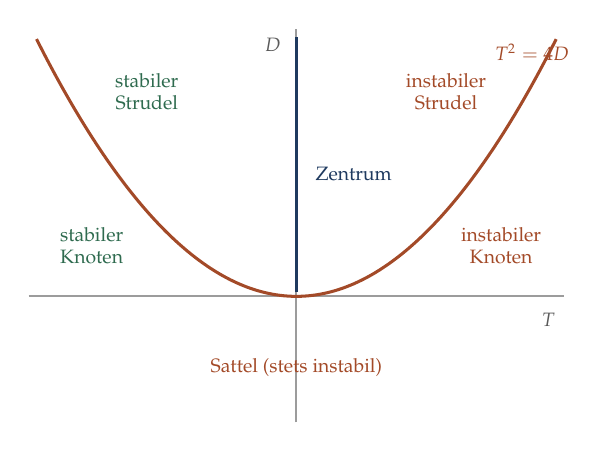
\begin{tikzpicture}[scale=1.0]
\draw[grau!60, line width=0.7pt] (-3.4,0) -- (3.4,0);
\draw[grau!60, line width=0.7pt] (0,-1.6) -- (0,3.4);
\draw[akzent, line width=1.1pt, smooth, samples=60, domain=-3.3:3.3]
  plot (\x, {0.3*\x*\x});
\node[font=\scriptsize, color=akzent, anchor=west] at (2.4,3.1) {$T^2 = 4D$};
\node[font=\scriptsize, color=grau] at (3.2,-0.3) {$T$};
\node[font=\scriptsize, color=grau] at (-0.3,3.2) {$D$};
\node[font=\scriptsize, color=gruen, align=center] at (-1.9,2.6) {stabiler\\Strudel};
\node[font=\scriptsize, color=akzent, align=center] at (1.9,2.6) {instabiler\\Strudel};
\node[font=\scriptsize, color=gruen, align=center] at (-2.6,0.65) {stabiler\\Knoten};
\node[font=\scriptsize, color=akzent, align=center] at (2.6,0.65) {instabiler\\Knoten};
\node[font=\scriptsize, color=akzent] at (0,-0.9) {Sattel (stets instabil)};
\draw[tief, line width=1.3pt] (0,0.05) -- (0,3.3);
\node[font=\scriptsize, color=tief, anchor=west] at (0.12,1.55) {Zentrum};
\end{tikzpicture}
\end{center}

\begin{center}
{\small
\renewcommand{\arraystretch}{1.5}
\begin{tabular}{@{}P{2.4cm}P{2.6cm}P{3.0cm}@{}}
\toprule
\textbf{Typ} & \textbf{Bedingung} & \textbf{Verhalten}\\
\midrule
Sattel & $D < 0$ & \textcolor{akzent}{zwei Richtungen, eine flieht}\\
Knoten & $D>0$, $T^2>4D$ & direkt hin oder weg\\
Strudel & $D>0$, $T^2<4D$ & \textcolor{mittel}{spiralig, schwingend}\\
Zentrum & $D>0$, $T=0$ & \textcolor{tief}{geschlossene Bahnen}\\
\bottomrule
\end{tabular}}
\end{center}
\end{merksatz}

\section{Die beiden Modelle geprüft}

\begin{merksatz}
\boxtitel{Lotka-Volterra --- warum ein Zentrum}
\[ f = x(a-by), \qquad g = y(-c+dx) \]

\schritt{Die Ableitungen}
\begin{align*}
\frac{\partial f}{\partial x} &= a - by & \frac{\partial f}{\partial y} &= -bx\\
\frac{\partial g}{\partial x} &= dy & \frac{\partial g}{\partial y} &= -c + dx
\end{align*}

\schritt{Im Gleichgewichtspunkt $\left(\frac{c}{d},\ \frac{a}{b}\right)$}
\[ \frac{\partial f}{\partial x} = a - b\cdot\frac{a}{b} = 0, \qquad \frac{\partial g}{\partial y} = -c + d\cdot\frac{c}{d} = 0 \]
\[ \frac{\partial f}{\partial y} = -\frac{bc}{d}, \qquad \frac{\partial g}{\partial x} = \frac{da}{b} \]

\[ J = \begin{pmatrix} 0 & -\frac{bc}{d}\\[4pt] \frac{da}{b} & 0 \end{pmatrix} \]

\schritt{Spur und Determinante}
\[ T = 0 + 0 = 0 \]
\[ D = 0\cdot0 - \left(-\frac{bc}{d}\right)\left(\frac{da}{b}\right) = +\,\frac{bc}{d}\cdot\frac{da}{b} = a\,c \]

\schritt{Das Ergebnis}
$T = 0$ und $D = ac > 0$: \textbf{ein Zentrum.}
\[ \lambda_{1,2} = \pm\mathrm{i}\sqrt{ac} \]

\begin{center}
\begin{minipage}{0.88\textwidth}
\kursiv{Damit ist die Periode aus Kapitel~4 begründet: Bei rein imaginären Eigenwerten $\pm\mathrm{i}\omega$ schwingt das System mit der Kreisfrequenz $\omega = \sqrt{ac}$, also der Periode $2\pi/\sqrt{ac}$. \checkmark}
\end{minipage}
\end{center}

\schritt{Und warum das so empfindlich ist}
Der Fall $T = 0$ ist genau der unentschiedene Fall aus Satz 6.2. Die Linearisierung sagt \enquote{Zentrum}, aber sie kann es nicht garantieren --- die vernachlässigten Terme entscheiden.

\begin{center}
\begin{minipage}{0.9\textwidth}
\textbf{Im Bild von Abschnitt 6.3 liegt das Zentrum genau auf der senkrechten Achse.} Jede noch so kleine Änderung schiebt den Punkt nach links oder rechts --- und macht daraus einen Strudel.
\end{minipage}
\end{center}

\begin{center}
\begin{minipage}{0.88\textwidth}
\kursiv{Das ist die strukturelle Instabilität aus Kapitel~4, nun in einem Satz begründet: Zentren sind Grenzfälle, und Grenzfälle sind fragil. Beim Lotka-Volterra-Modell rettet die Erhaltungsgröße aus Satz 4.3 das Zentrum --- aber nur, solange man das Modell nicht anrührt.}
\end{minipage}
\end{center}
\end{merksatz}

\begin{merksatz}
\boxtitel{Das Konkurrenzmodell --- Satz 5.3 nachgewiesen}
\[ f = r_1x\left(1 - \frac{x+\alpha_{12}y}{K_1}\right) \]

\schritt{Die Ableitungen}
Ausmultipliziert ist $f = r_1x - \frac{r_1}{K_1}x^2 - \frac{r_1\alpha_{12}}{K_1}xy$, also
\[ \frac{\partial f}{\partial x} = r_1 - \frac{2r_1}{K_1}x - \frac{r_1\alpha_{12}}{K_1}y, \qquad \frac{\partial f}{\partial y} = -\frac{r_1\alpha_{12}}{K_1}x \]

\schritt{Im Koexistenzpunkt}
Dort gilt $x^{*}+\alpha_{12}y^{*} = K_1$. Wir schreiben die erste Ableitung um:
\[ \frac{\partial f}{\partial x} = r_1\left(1 - \frac{x^{*}+\alpha_{12}y^{*}}{K_1} - \frac{x^{*}}{K_1}\right) = r_1\left(1 - 1 - \frac{x^{*}}{K_1}\right) = -\frac{r_1x^{*}}{K_1} \]

Entsprechend für $g$. Insgesamt
\[ J = \begin{pmatrix}
-\frac{r_1x^{*}}{K_1} & -\frac{r_1\alpha_{12}x^{*}}{K_1}\\[6pt]
-\frac{r_2\alpha_{21}y^{*}}{K_2} & -\frac{r_2y^{*}}{K_2}
\end{pmatrix} \]

\schritt{Die Spur}
\[ T = -\frac{r_1x^{*}}{K_1} - \frac{r_2y^{*}}{K_2} \;<\; 0 \]
--- stets negativ, da alle Größen positiv sind.

\schritt{Die Determinante}
\begin{align*}
D &= \frac{r_1x^{*}}{K_1}\cdot\frac{r_2y^{*}}{K_2} - \frac{r_1\alpha_{12}x^{*}}{K_1}\cdot\frac{r_2\alpha_{21}y^{*}}{K_2}\\
&= \frac{r_1r_2x^{*}y^{*}}{K_1K_2}\Bigl(1 - \alpha_{12}\alpha_{21}\Bigr)
\end{align*}

\schritt{Das Ergebnis}
\begin{center}
\begin{minipage}{0.9\textwidth}
\textbf{$D > 0$ genau dann, wenn $\alpha_{12}\alpha_{21} < 1$.} Und da $T$ ohnehin negativ ist, ist der Koexistenzpunkt genau unter dieser Bedingung stabil.
\end{minipage}
\end{center}

\begin{center}
\begin{minipage}{0.88\textwidth}
\kursiv{Damit ist Satz 5.3 sauber bewiesen, statt aus dem Bild abgelesen. Und man sieht zugleich, warum in Fall~4 ein Sattelpunkt vorliegt: Dort ist $\alpha_{12}\alpha_{21} > 1$, also $D < 0$.}
\end{minipage}
\end{center}
\end{merksatz}

\begin{merksatz}
\boxtitel{Mit den Zahlen aus Aufgabe 5.1}
$K_1=10$, $K_2=8$, $\alpha_{12}=0{,}6$, $\alpha_{21}=0{,}5$, $x^{*}=7{,}43$, $y^{*}=4{,}29$; dazu $r_1 = 1{,}0$, $r_2 = 0{,}8$.

\schritt{Die Matrix}
\[ J = \begin{pmatrix} -0{,}743 & -0{,}446\\ -0{,}215 & -0{,}429 \end{pmatrix} \]

\kursiv{Beispiel:} $-\frac{r_2\alpha_{21}y^{*}}{K_2} = -\frac{0{,}8 \cdot 0{,}5 \cdot 4{,}29}{8} = -\frac{1{,}716}{8} = -0{,}215$.

\schritt{Spur, Determinante, Diskriminante}
\[ T = -0{,}743 - 0{,}429 = -1{,}172 \]
\[ D = (-0{,}743)(-0{,}429) - (-0{,}446)(-0{,}215) = 0{,}3187 - 0{,}0959 = 0{,}2228 \]
\[ T^2 - 4D = 1{,}3736 - 0{,}8912 = 0{,}4824 > 0 \]

\schritt{Die Einordnung}
$D>0$, $T<0$, Diskriminante positiv: \textbf{stabiler Knoten.}

\schritt{Die Eigenwerte}
\[ \lambda_{1,2} = \frac{-1{,}172 \pm 0{,}6946}{2} \quad\Longrightarrow\quad \lambda_1 = -0{,}239,\quad \lambda_2 = -0{,}933 \]

\schritt{Die Probe}
$\lambda_1 + \lambda_2 = -1{,}172 = T$ \checkmark\\
$\lambda_1 \cdot \lambda_2 = 0{,}2230 \approx D$ \checkmark

\schritt{Die Deutung}
Die langsamere Annäherung erfolgt mit Rate $0{,}239$, also mit einer Halbwertszeit von
\[ \frac{\ln 2}{0{,}239} = 2{,}90 \ \text{Zeiteinheiten} . \]
Nach etwa vier solchen Zeiten --- rund zwölf Einheiten --- ist das Gleichgewicht praktisch erreicht. Das ist dieselbe Vier-Halbwertszeiten-Regel wie in Kapitel~1.
\end{merksatz}

\section{Der Bruchfall}

\begin{warnung}
\boxtitelr{Wo die Linearisierung nichts sagt}
\begin{center}
{\small
\renewcommand{\arraystretch}{1.52}
\begin{tabular}{@{}P{2.6cm}P{6.0cm}@{}}
\toprule
\textbf{Realteil null} & Der unentschiedene Fall aus Satz 6.2. Die Näherung sagt \enquote{Zentrum}, die Wirklichkeit kann eine langsam auslaufende oder aufklingende Spirale sein.\\
\textbf{Weit weg} & Die Aussage gilt nur \kursiv{nahe} dem Gleichgewicht. Wie nahe, sagt sie nicht.\\
\textbf{Mehrere Gleichgewichte} & Jedes wird einzeln untersucht; welches erreicht wird, bleibt offen.\\
\bottomrule
\end{tabular}}
\end{center}

\schritt{Zur zweiten Zeile}
Das ist die wichtigste Einschränkung. Ein stabiles Gleichgewicht kann ein winziges Einzugsgebiet haben.

\begin{center}
\begin{minipage}{0.88\textwidth}
\kursiv{Im Konkurrenzmodell Fall~4 sind beide Randzustände stabil --- und trotzdem landet man je nach Start bei verschiedenen. Die Stabilitätsuntersuchung sagt nichts darüber, wo die Grenze verläuft. Dafür braucht man die Bahn durch den Sattelpunkt, und die muss man ausrechnen.}
\end{minipage}
\end{center}
\end{warnung}

\begin{merksatz}
\boxtitel{Was sich beim Verändern eines Parameters ereignet}
Verschiebt man einen Parameter langsam, so wandert der Punkt $(T,D)$ durch das Bild aus Abschnitt 6.3. Überquert er eine Grenzlinie, ändert sich das Verhalten schlagartig. Man nennt das eine \Begriff{Bifurkation}.

\begin{center}
{\small
\renewcommand{\arraystretch}{1.5}
\begin{tabular}{@{}P{2.6cm}P{2.6cm}P{3.0cm}@{}}
\toprule
\textbf{Übergang} & \textbf{Grenze} & \textbf{Folge}\\
\midrule
Sattel-Knoten & $D = 0$ & zwei Gleichgewichte verschmelzen und verschwinden\\
Hopf & $T = 0$, $D>0$ & \textcolor{akzent}{aus Ruhe wird Schwingung}\\
Knoten-Strudel & $T^2 = 4D$ & nur die Form ändert sich\\
\bottomrule
\end{tabular}}
\end{center}

\begin{center}
\begin{minipage}{0.88\textwidth}
\kursiv{Die dritte Zeile ist harmlos --- die Stabilität ändert sich nicht. Die ersten beiden sind es nicht. Bei der Hopf-Bifurkation entsteht aus einem stabilen Ruhezustand eine anhaltende Schwingung; das ist der Weg, auf dem biologische Rhythmen in Modellen entstehen. Kapitel~12 zeigt es an der Erregung von Nervenzellen.}
\end{minipage}
\end{center}
\end{merksatz}

\begin{warnung}
\boxtitelr{Langsames Ankündigen}
Nähert sich ein System einer Bifurkation, so wird die Rückkehr nach einer Störung immer langsamer --- weil der maßgebliche Eigenwert gegen null geht.

\begin{center}
\begin{minipage}{0.9\textwidth}
\textbf{Das ist messbar, bevor der Übergang geschieht.} Wachsende Schwankungen und langsamere Erholung gelten als Frühwarnzeichen für einen bevorstehenden Umschlag.
\end{minipage}
\end{center}

\begin{center}
\begin{minipage}{0.88\textwidth}
\kursiv{Das Verfahren wird bei Ökosystemen, Klimakipppunkten und in der Medizin untersucht --- etwa bei der Frage, ob sich ein epileptischer Anfall oder ein Stimmungsumschwung ankündigt. Die Ergebnisse sind uneinheitlich: Das Zeichen tritt auf, ist aber wenig spezifisch. Kapitel~15 kommt darauf zurück.}
\end{minipage}
\end{center}
\end{warnung}

\section{Übungsaufgaben}

\begin{aufgabe}
\boxtitel{Aufgabe 6.1 --- Vier Systeme einordnen}
Bestimmen Sie Typ und Stabilität für die Matrizen
\[ J_1 = \begin{pmatrix} -2 & 1\\ 0 & -3\end{pmatrix},\quad
J_2 = \begin{pmatrix} 1 & 2\\ 3 & -1\end{pmatrix},\quad
J_3 = \begin{pmatrix} -1 & -4\\ 2 & -1\end{pmatrix},\quad
J_4 = \begin{pmatrix} 0 & -2\\ 3 & 0\end{pmatrix} . \]

\loesung
\schritt{$J_1$}
\[ T = -2 + (-3) = -5, \qquad D = (-2)(-3) - (1)(0) = 6 \]
\[ T^2-4D = 25 - 24 = 1 > 0 \]
$D>0$, $T<0$, Diskriminante positiv: \textbf{stabiler Knoten.}
\[ \lambda = \frac{-5 \pm 1}{2} = -2 \ \text{und}\ -3 \]
\kursiv{Probe:} Summe $-5$ \checkmark, Produkt $6$ \checkmark

\schritt{$J_2$}
\[ T = 1 + (-1) = 0, \qquad D = (1)(-1) - (2)(3) = -1 - 6 = -7 \]
$D < 0$: \textbf{Sattelpunkt, instabil.}
\[ T^2-4D = 0 + 28 = 28, \qquad \lambda = \frac{0 \pm 5{,}292}{2} = \pm2{,}646 \]
Ein positiver und ein negativer Eigenwert --- das Kennzeichen des Sattels.

\begin{center}
\begin{minipage}{0.86\textwidth}
\kursiv{Beachten Sie, dass hier $T = 0$ ist und der Punkt trotzdem eindeutig eingeordnet werden kann. Der unentschiedene Fall aus Satz 6.2 tritt nur ein, wenn $T=0$ \kursiv{und} $D>0$.}
\end{minipage}
\end{center}

\schritt{$J_3$}
\[ T = -1 + (-1) = -2, \qquad D = (-1)(-1) - (-4)(2) = 1 + 8 = 9 \]
\[ T^2-4D = 4 - 36 = -32 < 0 \]
$D>0$, $T<0$, Diskriminante negativ: \textbf{stabiler Strudel.}
\[ \lambda = \frac{-2 \pm \mathrm{i}\sqrt{32}}{2} = -1 \pm 2{,}828\,\mathrm{i} \]

\kursiv{Deutung:} Abklingrate $1$, Kreisfrequenz $2{,}828$, also Periode $2\pi/2{,}828 = 2{,}22$. Die Schwingung klingt mit der Halbwertszeit $\ln2/1 = 0{,}693$ ab --- deutlich schneller als eine Periode. Man sieht also kaum eine Schwingung, eher ein einmaliges Überschwingen.

\schritt{$J_4$}
\[ T = 0, \qquad D = 0 - (-2)(3) = 6 > 0 \]
$T=0$ und $D>0$: \textbf{Zentrum} --- und damit der \textcolor{akzent}{unentschiedene Fall}.
\[ \lambda = \pm\mathrm{i}\sqrt{6} = \pm2{,}449\,\mathrm{i} \]

\begin{center}
\begin{minipage}{0.86\textwidth}
\kursiv{Für die linearisierte Gleichung liegen geschlossene Bahnen vor. Ob das ursprüngliche nichtlineare System ebenfalls ein Zentrum hat, lässt sich daraus \kursiv{nicht} schließen.}
\end{minipage}
\end{center}

\schritt{Die Übersicht}
\begin{center}
\renewcommand{\arraystretch}{1.45}
\begin{tabular}{@{}P{1.2cm}P{1.4cm}P{1.4cm}P{1.6cm}P{2.4cm}@{}}
\toprule
& $T$ & $D$ & $T^2-4D$ & \textbf{Typ}\\
\midrule
$J_1$ & $-5$ & $6$ & $+1$ & stabiler Knoten\\
$J_2$ & $0$ & $-7$ & $+28$ & Sattel\\
$J_3$ & $-2$ & $9$ & $-32$ & stabiler Strudel\\
$J_4$ & $0$ & $6$ & $-24$ & Zentrum\\
\bottomrule
\end{tabular}
\end{center}
\end{aufgabe}

\begin{aufgabe}
\boxtitel{Aufgabe 6.2 --- Lotka-Volterra mit Kapazitätsgrenze}
Untersuchen Sie
\[ \frac{\dd x}{\dd t} = x\left(a\left(1-\frac{x}{K}\right) - by\right), \qquad \frac{\dd y}{\dd t} = y(-c+dx) \]
für $a=1{,}0$, $b=0{,}5$, $c=0{,}4$, $d=0{,}2$, $K=10$.

\loesung
\schritt{Schritt 1 --- Das Gleichgewicht}
Aus der zweiten Gleichung, mit $y \neq 0$:
\[ x^{*} = \frac{c}{d} = \frac{0{,}4}{0{,}2} = 2{,}0 \]
--- unverändert gegenüber Kapitel~4.

Aus der ersten, mit $x \neq 0$:
\[ a\left(1-\frac{x^{*}}{K}\right) = b\,y^{*} \quad\Longrightarrow\quad y^{*} = \frac{a}{b}\left(1-\frac{x^{*}}{K}\right) = \frac{1{,}0}{0{,}5}\left(1-\frac{2}{10}\right) = 2 \cdot 0{,}8 = 1{,}6 \]

\begin{center}
\begin{minipage}{0.86\textwidth}
\kursiv{Der Beutebestand bleibt bei $2{,}0$ --- die Überkreuz-Eigenschaft aus Kapitel~4 überlebt die Erweiterung. Der Räuberbestand sinkt von $2{,}0$ auf $1{,}6$, weil die Beute nun selbst begrenzt ist und weniger nachliefert.}
\end{minipage}
\end{center}

\schritt{Schritt 2 --- Die Ableitungen}
Ausmultipliziert: $f = ax - \frac{a}{K}x^2 - bxy$.
\[ \frac{\partial f}{\partial x} = a - \frac{2a}{K}x - by, \qquad \frac{\partial f}{\partial y} = -bx \]
\[ \frac{\partial g}{\partial x} = dy, \qquad \frac{\partial g}{\partial y} = -c+dx \]

\schritt{Schritt 3 --- Im Gleichgewicht einsetzen}
\[ \frac{\partial f}{\partial x} = 1{,}0 - \frac{2\cdot1{,}0}{10}\cdot2{,}0 - 0{,}5\cdot1{,}6 = 1{,}0 - 0{,}4 - 0{,}8 = -0{,}2 \]
\[ \frac{\partial f}{\partial y} = -0{,}5 \cdot 2{,}0 = -1{,}0 \]
\[ \frac{\partial g}{\partial x} = 0{,}2 \cdot 1{,}6 = 0{,}32 \]
\[ \frac{\partial g}{\partial y} = -0{,}4 + 0{,}2\cdot2{,}0 = 0 \]

\[ J = \begin{pmatrix} -0{,}2 & -1{,}0\\ 0{,}32 & 0 \end{pmatrix} \]

\schritt{Schritt 4 --- Einordnen}
\[ T = -0{,}2 + 0 = -0{,}2 \]
\[ D = (-0{,}2)(0) - (-1{,}0)(0{,}32) = 0{,}32 \]
\[ T^2-4D = 0{,}04 - 1{,}28 = -1{,}24 < 0 \]

$D>0$, $T<0$, Diskriminante negativ: \textbf{stabiler Strudel.}

\schritt{Schritt 5 --- Die Eigenwerte}
\[ \lambda = \frac{-0{,}2 \pm \mathrm{i}\sqrt{1{,}24}}{2} = -0{,}1 \pm 0{,}557\,\mathrm{i} \]

\schritt{Schritt 6 --- Die Deutung}
\begin{center}
\renewcommand{\arraystretch}{1.48}
\begin{tabular}{@{}P{2.8cm}P{2.4cm}P{2.4cm}@{}}
\toprule
& \textbf{Wert} & \\
\midrule
Abklingrate & $0{,}1\ \mathrm{h}^{-1}$ & \\
Halbwertszeit & $6{,}93$ h & $\ln2/0{,}1$\\
Kreisfrequenz & $0{,}557$ & \\
Periode & $11{,}3$ h & $2\pi/0{,}557$\\
\bottomrule
\end{tabular}
\end{center}

Die Schwingung hat eine Periode von etwa elf Stunden und klingt mit einer Halbwertszeit von sieben Stunden ab. Nach etwa vier Perioden ist sie praktisch verschwunden.

\schritt{Schritt 7 --- Der Vergleich mit Kapitel 4}
\begin{center}
\renewcommand{\arraystretch}{1.48}
\begin{tabular}{@{}P{2.8cm}P{2.4cm}P{2.4cm}@{}}
\toprule
& \textbf{ohne $K$} & \textbf{mit $K$}\\
\midrule
$T$ & $0$ & $\mathbf{-0{,}2}$\\
Typ & Zentrum & \textcolor{gruen}{stabiler Strudel}\\
Periode & $9{,}93$ h & $11{,}3$ h\\
\bottomrule
\end{tabular}
\end{center}

\begin{center}
\begin{minipage}{0.88\textwidth}
\kursiv{Damit ist der Bruchfall aus Kapitel~4 nachgewiesen statt behauptet: Die Kapazitätsgrenze verschiebt die Spur von null ins Negative, und aus dem Zentrum wird ein Strudel. \textbf{Die Ursache steckt allein im Term $-\frac{2a}{K}x$}, der bei $K \to \infty$ verschwindet --- dann wäre $T=0$ wie zuvor.}
\end{minipage}
\end{center}
\end{aufgabe}

\begin{aufgabe}
\boxtitel{Aufgabe 6.3 --- Eine Bifurkation aufspüren}
Für das System aus Aufgabe 6.2 sei $K$ veränderlich. Bei welchem $K$ ändert sich das Verhalten qualitativ, und was geschieht?

\loesung
\schritt{Schritt 1 --- Das Gleichgewicht allgemein}
\[ x^{*} = \frac{c}{d} = 2{,}0 \ \text{(von $K$ unabhängig)}, \qquad y^{*} = \frac{a}{b}\left(1-\frac{2}{K}\right) = 2\left(1-\frac{2}{K}\right) \]

\schritt{Schritt 2 --- Die erste Bedingung}
Damit $y^{*} > 0$ ist, muss
\[ 1 - \frac{2}{K} > 0 \quad\Longleftrightarrow\quad K > 2 . \]

\begin{center}
\begin{minipage}{0.9\textwidth}
\textbf{Bei $K = 2$ verschwindet der Räuber.} Ist die Kapazität der Beute nicht größer als der Bedarf des Räubers, so kann er nicht bestehen.
\end{minipage}
\end{center}

\schritt{Schritt 3 --- Die Spur allgemein}
\[ \frac{\partial f}{\partial x}\Big|_{*} = a - \frac{2a}{K}x^{*} - by^{*} \]
Mit $by^{*} = a\left(1-\frac{x^{*}}{K}\right)$:
\[ = a - \frac{2a x^{*}}{K} - a + \frac{ax^{*}}{K} = -\frac{a\,x^{*}}{K} \]

Da $\frac{\partial g}{\partial y} = 0$ im Gleichgewicht:
\[ T = -\frac{a\,x^{*}}{K} = -\frac{1{,}0 \cdot 2{,}0}{K} = -\frac{2}{K} \]

\schritt{Schritt 4 --- Die Determinante allgemein}
\[ D = 0 - (-b x^{*})(d y^{*}) = b\,d\,x^{*}y^{*} = 0{,}5 \cdot 0{,}2 \cdot 2{,}0 \cdot y^{*} = 0{,}2\,y^{*} \]
\[ = 0{,}2 \cdot 2\left(1-\frac{2}{K}\right) = 0{,}4\left(1-\frac{2}{K}\right) \]

\schritt{Schritt 5 --- Die Werte im Überblick}
\begin{center}
{\small
\renewcommand{\arraystretch}{1.48}
\begin{tabular}{@{}P{1.4cm}P{1.6cm}P{1.8cm}P{1.6cm}P{2.0cm}@{}}
\toprule
$K$ & $y^{*}$ & $T$ & $D$ & \textbf{Typ}\\
\midrule
$2{,}5$ & $0{,}40$ & $-0{,}800$ & $0{,}080$ & Knoten\\
$3{,}0$ & $0{,}67$ & $-0{,}667$ & $0{,}133$ & Knoten\\
$4{,}0$ & $1{,}00$ & $-0{,}500$ & $0{,}200$ & \textcolor{akzent}{Grenze}\\
$6{,}0$ & $1{,}33$ & $-0{,}333$ & $0{,}267$ & Strudel\\
$10{,}0$ & $1{,}60$ & $-0{,}200$ & $0{,}320$ & Strudel\\
$\infty$ & $2{,}00$ & $\mathbf{0}$ & $0{,}400$ & \textcolor{tief}{Zentrum}\\
\bottomrule
\end{tabular}}
\end{center}

\schritt{Schritt 6 --- Die Grenze bestimmen}
Der Übergang Knoten/Strudel liegt bei $T^2 = 4D$:
\[ \frac{4}{K^2} = 4 \cdot 0{,}4\left(1-\frac{2}{K}\right) = 1{,}6 - \frac{3{,}2}{K} \]
Mit $K^2$ multiplizieren:
\[ 4 = 1{,}6K^2 - 3{,}2K \quad\Longrightarrow\quad 1{,}6K^2 - 3{,}2K - 4 = 0 \]
\[ K^2 - 2K - 2{,}5 = 0 \quad\Longrightarrow\quad K = 1 \pm \sqrt{1+2{,}5} = 1 \pm 1{,}871 \]
Die positive Lösung: $K = 2{,}871$.

\kursiv{Kontrolle:} Bei $K=4$ ist $T^2 = 0{,}25$ und $4D = 0{,}80$ --- also bereits Strudel. Bei $K=2{,}5$ ist $T^2=0{,}64$ und $4D=0{,}32$ --- Knoten. Die Grenze liegt dazwischen. \checkmark

\schritt{Schritt 7 --- Die Zusammenfassung}
\begin{center}
{\small
\renewcommand{\arraystretch}{1.48}
\begin{tabular}{@{}P{2.6cm}P{5.8cm}@{}}
\toprule
$K \le 2$ & Der Räuber stirbt aus; die Beute strebt gegen $K$.\\
$2 < K < 2{,}87$ & Stabiler Knoten --- Annäherung ohne Schwingen.\\
$K > 2{,}87$ & Stabiler Strudel --- gedämpfte Schwingungen.\\
$K \to \infty$ & Zentrum --- ungedämpfte Schwingungen.\\
\bottomrule
\end{tabular}}
\end{center}

\schritt{Schritt 8 --- Die Deutung}
\begin{center}
\begin{minipage}{0.9\textwidth}
\textbf{Je reicher die Umwelt --- je größer $K$ ---, desto schwächer gedämpft sind die Schwingungen.}
\end{minipage}
\end{center}

\begin{center}
\begin{minipage}{0.88\textwidth}
\kursiv{Dieses Ergebnis ist der Kern des sogenannten \Begriff{Anreicherungsparadoxons}: Verbessert man die Lebensbedingungen der Beute, so wird das System \kursiv{instabiler}, nicht stabiler. Bei realistischeren Fraßfunktionen kippt es sogar ganz um --- die Schwingungen wachsen an, bis eine Art ausstirbt. Rosenzweig beschrieb das 1971; es gilt als eines der überraschendsten Ergebnisse der theoretischen Ökologie.}
\end{minipage}
\end{center}
\end{aufgabe}

\begin{geschichte}
\boxtitelg{Zwei Wege zur selben Frage}
Die Frage, ob ein Gleichgewicht stabil ist, stellte sich zuerst in der Himmelsmechanik: Bleibt das Sonnensystem, wie es ist?

\Person{Henri Poincaré} (1854--1912) entwickelte ab 1881 die Methoden, die dieses Kapitel benutzt --- Phasenporträt, Nullklinen, Einordnung der Gleichgewichte. Er tat es, weil er die Bahnen nicht ausrechnen konnte und deshalb einen Weg suchte, ihr Verhalten \kursiv{ohne} Lösung zu bestimmen.

\begin{center}
\begin{minipage}{0.9\textwidth}
\kursiv{Poincaré fand dabei auch die empfindliche Abhängigkeit von den Anfangsbedingungen --- siebzig Jahre vor Lorenz. In der Preisschrift von 1890 über das Dreikörperproblem beschreibt er Bahnen von einer Verwicklung, die er selbst nicht zeichnen zu können erklärte. Die Stelle wurde jahrzehntelang übersehen.}
\end{minipage}
\end{center}

\Person{Alexander Ljapunow} (1857--1918) bewies 1892 in seiner Dissertation, dass die Linearisierung tatsächlich entscheidet --- sofern kein Realteil null ist. Das ist genau der Vorbehalt aus Satz 6.2, und er stammt von ihm.

\begin{center}
\begin{minipage}{0.9\textwidth}
\kursiv{Ljapunow entwickelte daneben eine zweite Methode, die ohne Linearisierung auskommt: Man sucht eine Funktion, die entlang jeder Bahn abnimmt --- ähnlich der Erhaltungsgröße aus Satz 4.3, nur mit Ungleichung statt Gleichung. Diese \enquote{direkte Methode} gilt bis heute als das mächtigste Stabilitätswerkzeug.}
\end{minipage}
\end{center}

\schritt{Der Weg in die Biologie}
Poincaré und Ljapunow arbeiteten an Himmelsmechanik und Regelungstechnik. Dass ihre Werkzeuge auf Populationen passen, bemerkte man erst in den 1920er Jahren --- durch Lotka und Volterra.

\begin{center}
\begin{minipage}{0.9\textwidth}
\kursiv{Das ist ein wiederkehrendes Muster: Die mathematischen Mittel sind lange vor ihrer Anwendung da. Beim Chaos war es dieselbe Lage --- Poincaré 1890, Verwendung ab 1975.}
\end{minipage}
\end{center}
\end{geschichte}

\begin{forschung}
\boxtitelp{Stabilität heute}
\begin{center}
{\small
\renewcommand{\arraystretch}{1.45}
\begin{tabular}{@{}P{2.8cm}P{5.4cm}@{}}
\toprule
\textbf{Viele Arten} & Bei $n$ Arten ist $J$ eine $n\times n$-Matrix. Robert May zeigte 1972, dass zufällig verknüpfte große Systeme mit wachsender Artenzahl \kursiv{instabiler} werden --- entgegen der damaligen Lehrmeinung.\\
\textbf{Netzwerk\-struktur} & Die Auflösung des Widerspruchs: Echte Nahrungsnetze sind nicht zufällig verknüpft. Welche Strukturen stabilisieren, ist ein aktives Feld.\\
\textbf{Frühwarnzeichen} & Langsamere Erholung und wachsende Schwankungen vor Kipppunkten; geprüft an Seen, Klimadaten und medizinischen Zeitreihen.\\
\bottomrule
\end{tabular}}
\end{center}

Mays Ergebnis von 1972 ist ein Musterbeispiel dafür, wie ein mathematischer Befund ein Fach erschüttert. Die Ökologie hatte jahrzehntelang gelehrt, Vielfalt erzeuge Stabilität. May rechnete nach und fand das Gegenteil --- für zufällig verknüpfte Systeme.

\begin{center}
\begin{minipage}{0.88\textwidth}
\kursiv{Die Auflösung dauerte dreißig Jahre und lautet: Beides ist richtig, je nach Struktur. Vielfalt stabilisiert, wenn die Verknüpfungen bestimmten Mustern folgen --- viele schwache und wenige starke Wechselwirkungen, geschachtelte Nahrungsnetze. Zufällige Vielfalt destabilisiert. Das ist ein Ergebnis, das ohne die Matrixrechnung dieses Kapitels nicht formulierbar wäre.}
\end{minipage}
\end{center}
\end{forschung}

\begin{merksatz}
\boxtitel{Was Sie jetzt können}
\begin{center}
\renewcommand{\arraystretch}{1.5}
\begin{tabular}{@{}P{3.0cm}P{5.6cm}@{}}
\toprule
\textbf{Definition 6.1} & Jacobi-Matrix als Tangente in zwei Veränderlichen\\
\textbf{Satz 6.2} & Vorzeichen der Realteile entscheidet\\
\textbf{Satz 6.3} & stabil $\iff$ $T<0$ und $D>0$\\
\textbf{Die Landkarte} & Sattel, Knoten, Strudel, Zentrum\\
\textbf{Zwei Nachweise} & Lotka-Volterra ist ein Zentrum; Satz 5.3 bewiesen\\
\bottomrule
\end{tabular}
\end{center}

\begin{center}
\begin{minipage}{0.88\textwidth}
\kursiv{Damit endet Teil~II. Ab Kapitel~7 wenden wir dieselben Werkzeuge auf eine Frage an, bei der eine einzige Zahl über Ausbruch oder Abklingen entscheidet.}
\end{minipage}
\end{center}
\end{merksatz}

\part{Ausbreitung}

\chapter{Das SIR-Modell}

\section{Der Leitfall}

\begin{merksatz}
\boxtitel{Neustadt}
Der Erreger aus dem Klinikum hat die Stadt erreicht. Neustadt hat $100\,000$ Einwohner. Eine Person bleibt etwa fünf Tage ansteckend; danach ist sie genesen und nicht mehr empfänglich.

\textbf{Die Fragen:}
\begin{center}
\renewcommand{\arraystretch}{1.48}
\begin{tabular}{@{}P{1.0cm}P{7.4cm}@{}}
\toprule
$1$ & Breitet sich der Erreger überhaupt aus?\\
$2$ & Wann ist der Höhepunkt, und wie viele sind dann gleichzeitig krank?\\
$3$ & Wie viele erkranken insgesamt?\\
\bottomrule
\end{tabular}
\end{center}

\begin{center}
\begin{minipage}{0.88\textwidth}
\kursiv{Alle drei Fragen lassen sich mit drei Gleichungen beantworten --- und die Antwort auf die erste hängt an einer einzigen Zahl.}
\end{minipage}
\end{center}
\end{merksatz}

\begin{merksatz}
\boxtitel{Die drei Kammern}
Man teilt die Bevölkerung in drei Gruppen ein:

\begin{center}
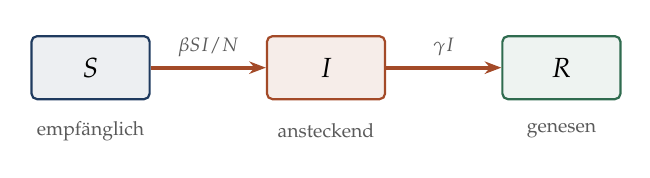
\begin{tikzpicture}[scale=1.15]
\node[draw=tief, thick, rounded corners=2pt, minimum width=1.5cm, minimum height=0.8cm, fill=tief!8] (S) at (-2.6,0) {$S$};
\node[draw=akzent, thick, rounded corners=2pt, minimum width=1.5cm, minimum height=0.8cm, fill=akzent!10] (I) at (0,0) {$I$};
\node[draw=gruen, thick, rounded corners=2pt, minimum width=1.5cm, minimum height=0.8cm, fill=gruen!8] (R) at (2.6,0) {$R$};
\draw[kanted, -{Stealth[length=6pt]}] (S) -- (I) node[midway, above, font=\scriptsize, color=grau] {$\beta SI/N$};
\draw[kanted, -{Stealth[length=6pt]}] (I) -- (R) node[midway, above, font=\scriptsize, color=grau] {$\gamma I$};
\node[font=\scriptsize, color=grau] at (-2.6,-0.7) {empfänglich};
\node[font=\scriptsize, color=grau] at (0,-0.7) {ansteckend};
\node[font=\scriptsize, color=grau] at (2.6,-0.7) {genesen};
\end{tikzpicture}
\end{center}

\begin{center}
{\small
\renewcommand{\arraystretch}{1.5}
\begin{tabular}{@{}P{1.4cm}P{2.6cm}P{4.4cm}@{}}
\toprule
$S$ & \kursiv{susceptible} & noch nicht angesteckt, kann es werden\\
$I$ & \kursiv{infectious} & angesteckt und ansteckend\\
$R$ & \kursiv{removed} & genesen oder gestorben --- in beiden Fällen aus dem Geschehen\\
\bottomrule
\end{tabular}}
\end{center}

\begin{center}
\begin{minipage}{0.88\textwidth}
\kursiv{Das $R$ steht für \kursiv{removed}, nicht für \kursiv{recovered}. Das ist keine Wortklauberei: Verstorbene und Genesene sind für die Ausbreitung gleichwertig --- beide stecken niemanden mehr an und können nicht erneut erkranken. Das Modell unterscheidet sie nicht.}
\end{minipage}
\end{center}
\end{merksatz}

\begin{merksatz}
\boxtitel{Die Annahmen --- alle sechs}
\begin{center}
{\small
\renewcommand{\arraystretch}{1.5}
\begin{tabular}{@{}P{0.7cm}P{7.7cm}@{}}
\toprule
$1$ & Die Bevölkerung ist \kursiv{gut durchmischt}: Jeder trifft jeden mit gleicher Wahrscheinlichkeit.\\
$2$ & Die Gesamtzahl $N = S+I+R$ bleibt fest --- keine Geburten, keine Zuwanderung.\\
$3$ & Genesene sind dauerhaft geschützt.\\
$4$ & Es gibt keine Inkubationszeit: Wer angesteckt wird, ist sofort ansteckend.\\
$5$ & Alle sind gleich ansteckend und gleich empfänglich.\\
$6$ & Die Ansteckungsrate ist proportional zu $S \cdot I$ --- das Massenwirkungsgesetz aus Kapitel~4.\\
\bottomrule
\end{tabular}}
\end{center}

\begin{center}
\begin{minipage}{0.88\textwidth}
\kursiv{Keine dieser sechs Annahmen trifft zu. Der Abschnitt über den Bruchfall geht jede einzeln durch. Erstaunlich ist, dass das Modell trotzdem brauchbare Auskünfte gibt --- und wichtig ist zu wissen, welche.}
\end{minipage}
\end{center}
\end{merksatz}

\begin{definition}
\boxtitelm{Definition 7.1 --- das SIR-Modell}
\[ \frac{\dd S}{\dd t} = -\beta\,\frac{S\,I}{N}, \qquad
\frac{\dd I}{\dd t} = \beta\,\frac{S\,I}{N} - \gamma\,I, \qquad
\frac{\dd R}{\dd t} = \gamma\,I \]
mit der \Begriff{Übertragungsrate} $\beta$ und der \Begriff{Genesungsrate} $\gamma$.
\end{definition}

\begin{merksatz}
\boxtitel{Die beiden Parameter}
\begin{center}
\renewcommand{\arraystretch}{1.5}
\begin{tabular}{@{}P{1.4cm}P{3.0cm}P{3.6cm}@{}}
\toprule
$\beta$ & Ansteckungen je Ansteckendem und Zeit, wenn alle empfänglich sind & $\mathrm{d}^{-1}$\\
$\gamma$ & Anteil der Ansteckenden, der je Zeiteinheit genest & $\mathrm{d}^{-1}$\\
$1/\gamma$ & \textbf{mittlere Ansteckungsdauer} & Tage\\
\bottomrule
\end{tabular}
\end{center}

\schritt{Warum $1/\gamma$ die Dauer ist}
Betrachtet man nur die zweite Gleichung ohne Neuansteckungen, so lautet sie $\dd I/\dd t = -\gamma I$ --- der Zerfall aus Kapitel~1. Die mittlere Verweildauer bei exponentiellem Zerfall beträgt $1/\gamma$.

\schritt{Die Probe: Bleibt $N$ fest?}
\[ \frac{\dd}{\dd t}(S+I+R) = -\beta\frac{SI}{N} + \beta\frac{SI}{N} - \gamma I + \gamma I = 0 . \quad \checkmark \]

\begin{center}
\begin{minipage}{0.88\textwidth}
\kursiv{Diese Probe sollte man bei jedem Kammermodell durchführen. Summieren sich die Ableitungen nicht zu null, so hat man einen Fluss vergessen oder doppelt gezählt --- der häufigste Fehler beim Aufstellen solcher Modelle.}
\end{minipage}
\end{center}

\schritt{Die dritte Gleichung ist überflüssig}
Da $R = N - S - I$, genügen die ersten beiden. Man führt $R$ trotzdem mit, weil es die Zahl der Genesenen liefert --- und weil die Probe sonst nicht möglich wäre.
\end{merksatz}

\section{Die Basisreproduktionszahl}

\begin{merksatz}
\boxtitel{Satz 7.2 --- die Schwellenbedingung}
Eine Epidemie breitet sich zu Beginn genau dann aus, wenn
\[ \Rnull \;:=\; \frac{\beta}{\gamma} \;>\; 1 . \]

\schritt{Beweis}
Ausbreitung bedeutet $\dd I/\dd t > 0$:
\[ \beta\frac{SI}{N} - \gamma I > 0 \]

Wir klammern $I$ aus --- es ist positiv, also dürfen wir teilen:
\[ I\left(\beta\frac{S}{N} - \gamma\right) > 0 \quad\Longleftrightarrow\quad \beta\frac{S}{N} > \gamma \quad\Longleftrightarrow\quad \frac{\beta}{\gamma}\cdot\frac{S}{N} > 1 \]

Zu Beginn ist fast die ganze Bevölkerung empfänglich, also $S/N \approx 1$:
\[ \frac{\beta}{\gamma} > 1 . \qquad \blacksquare \]
\end{merksatz}

\begin{merksatz}
\boxtitel{Was $\Rnull$ bedeutet}
\begin{center}
\begin{minipage}{0.9\textwidth}
\textbf{$\Rnull$ ist die mittlere Zahl der Personen, die ein Ansteckender in einer vollständig empfänglichen Bevölkerung ansteckt.}
\end{minipage}
\end{center}

\schritt{Warum $\beta/\gamma$ genau das ist}
Ein Ansteckender steckt je Zeiteinheit $\beta$ Personen an und bleibt im Mittel $1/\gamma$ lang ansteckend:
\[ \beta \cdot \frac{1}{\gamma} = \frac{\beta}{\gamma} = \Rnull . \]

\schritt{Die effektive Reproduktionszahl}
Während der Epidemie sind nicht mehr alle empfänglich. Man setzt
\[ \mathcal{R}_{\text{eff}}(t) = \Rnull\cdot\frac{S(t)}{N} . \]

\begin{center}
\renewcommand{\arraystretch}{1.48}
\begin{tabular}{@{}P{2.6cm}P{2.6cm}P{2.8cm}@{}}
\toprule
$\mathcal{R}_{\text{eff}}$ & \textbf{Fallzahl} & \\
\midrule
$> 1$ & \textcolor{akzent}{steigt} & Epidemie wächst\\
$= 1$ & \textcolor{mittel}{Höhepunkt} & Wendepunkt\\
$< 1$ & \textcolor{gruen}{fällt} & Epidemie klingt ab\\
\bottomrule
\end{tabular}
\end{center}

\begin{center}
\begin{minipage}{0.88\textwidth}
\kursiv{Die mittlere Zeile ist der Schlüssel zum Rest des Kapitels: Der Höhepunkt liegt genau dort, wo $\mathcal{R}_{\text{eff}} = 1$ wird --- also wo der Anteil der Empfänglichen auf $1/\Rnull$ gefallen ist. Das ist eine Bedingung, die man ausrechnen kann, ohne die Gleichungen zu lösen.}
\end{minipage}
\end{center}
\end{merksatz}

\begin{merksatz}
\boxtitel{Die Neustädter Zahlen}
\[ \frac{1}{\gamma} = 5\ \text{Tage} \quad\Longrightarrow\quad \gamma = 0{,}2\ \mathrm{d}^{-1} \]
\[ \Rnull = 2{,}5 \quad\Longrightarrow\quad \beta = \Rnull\,\gamma = 2{,}5 \cdot 0{,}2 = 0{,}5\ \mathrm{d}^{-1} \]

\schritt{Die Antwort auf Frage 1}
$\Rnull = 2{,}5 > 1$: \textbf{Die Epidemie breitet sich aus.}

\schritt{Das anfängliche Wachstum}
Solange $S \approx N$, lautet die zweite Gleichung
\[ \frac{\dd I}{\dd t} \approx (\beta - \gamma)\,I = 0{,}3\,I \]
--- exponentielles Wachstum aus Kapitel~1 mit $r = 0{,}3\ \mathrm{d}^{-1}$.

\[ T_2 = \frac{\ln 2}{0{,}3} = 2{,}31\ \text{Tage} \]

\begin{center}
\begin{minipage}{0.88\textwidth}
\kursiv{Die Verdopplungszeit ist die Größe, die in der Frühphase gemessen wird --- die Fallzahlen verdoppeln sich alle zweieinviertel Tage. Aus ihr und der bekannten Ansteckungsdauer lässt sich $\Rnull$ zurückrechnen: $\Rnull = 1 + r/\gamma = 1 + 0{,}3/0{,}2 = 2{,}5$. \checkmark}
\end{minipage}
\end{center}
\end{merksatz}

\section{Der Höhepunkt}

\begin{merksatz}
\boxtitel{Satz 7.3 --- die Höhe des Gipfels}
Beginnt die Epidemie mit $S_0 \approx N$ und $I_0 \approx 0$, so beträgt der größte gleichzeitige Krankenstand
\[ \frac{I_{\max}}{N} \;=\; 1 - \frac{1+\ln\Rnull}{\Rnull} . \]
\end{merksatz}

\begin{merksatz}
\boxtitel{Beweis --- die Zeit loswerden}
\schritt{Schritt 1 --- Zwei Gleichungen dividieren}
Wir fragen nicht nach $I(t)$, sondern nach $I$ als Funktion von $S$. Dazu teilen wir:
\[ \frac{\dd I}{\dd S} = \frac{\dd I/\dd t}{\dd S/\dd t} = \frac{\beta\frac{SI}{N} - \gamma I}{-\beta\frac{SI}{N}} \]

Im Zähler $I$ ausklammern, dann durch $\beta SI/N$ kürzen:
\[ = \frac{I\left(\beta\frac{S}{N}-\gamma\right)}{-\beta\frac{SI}{N}} = -1 + \frac{\gamma N}{\beta S} = -1 + \frac{N}{\Rnull\,S} \]

\begin{center}
\begin{minipage}{0.88\textwidth}
\kursiv{Der Kunstgriff ist, die Zeit durch Division zu beseitigen. Zurück bleibt eine gewöhnliche Differentialgleichung erster Ordnung, die sich unmittelbar integrieren lässt. Das ist derselbe Gedanke wie bei den Bahnkurven in Kapitel~4.}
\end{minipage}
\end{center}

\schritt{Schritt 2 --- Integrieren}
\[ I(S) = -S + \frac{N}{\Rnull}\ln S + C \]

\schritt{Schritt 3 --- Die Konstante}
Bei $S = S_0$ ist $I = I_0$:
\[ C = I_0 + S_0 - \frac{N}{\Rnull}\ln S_0 \]

\[ I(S) = I_0 + S_0 - S + \frac{N}{\Rnull}\ln\frac{S}{S_0} \]

\schritt{Schritt 4 --- Wo der Gipfel liegt}
Nach Satz 7.2 ist $\dd I/\dd t = 0$ genau dann, wenn
\[ S = \frac{N}{\Rnull} . \]

\schritt{Schritt 5 --- Einsetzen}
Mit $S_0 = N$ und $I_0 = 0$:
\[ I_{\max} = N - \frac{N}{\Rnull} + \frac{N}{\Rnull}\ln\frac{N/\Rnull}{N} = N - \frac{N}{\Rnull} - \frac{N}{\Rnull}\ln\Rnull \]
\[ \frac{I_{\max}}{N} = 1 - \frac{1}{\Rnull} - \frac{\ln\Rnull}{\Rnull} = 1 - \frac{1+\ln\Rnull}{\Rnull} . \qquad \blacksquare \]
\end{merksatz}

\begin{merksatz}
\boxtitel{Die Antwort auf Frage 2}
Für $\Rnull = 2{,}5$:
\[ \ln 2{,}5 = 0{,}9163 \]
\[ \frac{I_{\max}}{N} = 1 - \frac{1 + 0{,}9163}{2{,}5} = 1 - \frac{1{,}9163}{2{,}5} = 1 - 0{,}7665 = 0{,}2335 \]

\[ I_{\max} = 0{,}2335 \cdot 100\,000 = \mathbf{23\,350} \ \text{gleichzeitig Kranke} . \]

Der Gipfel wird erreicht, wenn $S = N/\Rnull = 40\,000$ --- also wenn $60\,\%$ der Bevölkerung bereits erkrankt oder erkrankend sind.

\schritt{Die Probe durch numerische Lösung}
Rechnet man die Gleichungen schrittweise durch, so ergibt sich der Gipfel am Tag $32{,}1$ mit $23\,367$ Kranken --- gegen $23\,348$ aus der Formel. Die Abweichung von $0{,}1\,\%$ stammt daher, dass die Epidemie mit zehn statt null Kranken begann. \checkmark

\begin{center}
\begin{minipage}{0.88\textwidth}
\kursiv{Bemerkenswert ist, was die Formel \kursiv{nicht} liefert: den Zeitpunkt. Er hängt vom Ausgangswert $I_0$ ab und lässt sich nicht geschlossen angeben. Die Höhe des Gipfels ist von $I_0$ praktisch unabhängig, sein Zeitpunkt nicht.}
\end{minipage}
\end{center}
\end{merksatz}

\section{Die Endgröße}

\begin{merksatz}
\boxtitel{Satz 7.4 --- wie viele insgesamt erkranken}
Sei $s_\infty = S_\infty/N$ der Anteil, der nie erkrankt. Dann gilt
\[ s_\infty = e^{-\Rnull\,(1-s_\infty)} . \]

\schritt{Beweis}
Am Ende ist $I = 0$. Aus der Gleichung in Schritt 3 des vorigen Beweises, mit $S_0 = N$ und $I_0 = 0$:
\[ 0 = N - S_\infty + \frac{N}{\Rnull}\ln\frac{S_\infty}{N} \]

Durch $N$ teilen und $s_\infty = S_\infty/N$ setzen:
\[ 0 = 1 - s_\infty + \frac{1}{\Rnull}\ln s_\infty \]
\[ \ln s_\infty = -\Rnull\,(1-s_\infty) \]
\[ s_\infty = e^{-\Rnull(1-s_\infty)} . \qquad \blacksquare \]

\schritt{Warum man das nicht auflösen kann}
Die Unbekannte steht innerhalb und außerhalb der Exponentialfunktion. Eine solche Gleichung hat keine geschlossene Lösung in den Grundfunktionen; man löst sie durch Iteration.
\end{merksatz}

\begin{merksatz}
\boxtitel{Die Antwort auf Frage 3}
Wir lösen $s = e^{-2{,}5(1-s)}$ durch wiederholtes Einsetzen, beginnend bei $s = 0{,}5$:

\begin{center}
{\small
\renewcommand{\arraystretch}{1.38}
\begin{tabular}{@{}P{1.2cm}P{2.0cm}P{1.2cm}P{2.0cm}@{}}
\toprule
Schritt & $s$ & Schritt & $s$\\
\midrule
$0$ & $0{,}5000$ & $5$ & $0{,}1140$\\
$1$ & $0{,}2865$ & $10$ & $0{,}1075$\\
$2$ & $0{,}1665$ & $20$ & $0{,}1073$\\
$3$ & $0{,}1244$ & $\infty$ & $\mathbf{0{,}1073}$\\
\bottomrule
\end{tabular}}
\end{center}

\schritt{Das Ergebnis}
\[ s_\infty = 0{,}1073 \quad\Longrightarrow\quad \text{Befallsrate} = 1 - 0{,}1073 = \mathbf{89{,}3\,\%} \]

Rund $89\,300$ Menschen erkranken; etwa $10\,700$ bleiben verschont.

\schritt{Die Probe}
\[ e^{-2{,}5(1-0{,}1073)} = e^{-2{,}5 \cdot 0{,}8927} = e^{-2{,}2318} = 0{,}1073 . \quad \checkmark \]
\end{merksatz}

\begin{warnung}
\boxtitelr{Das Überschwingen --- der wichtigste Befund dieses Kapitels}
Die Herdenschwelle liegt bei
\[ 1 - \frac{1}{\Rnull} = 1 - \frac{1}{2{,}5} = 0{,}60 , \]
also bei $60\,\%$. Ab dort sinkt $\mathcal{R}_{\text{eff}}$ unter eins und die Fallzahlen fallen.

\begin{center}
\begin{minipage}{0.9\textwidth}
\textbf{Trotzdem erkranken am Ende $89{,}3\,\%$ --- fast dreißig Prozentpunkte mehr als nötig.}
\end{minipage}
\end{center}

\schritt{Warum}
Beim Erreichen der Schwelle sind noch $23\,350$ Menschen ansteckend. Diese stecken weiter an --- nur eben jeder weniger als einen. Die Epidemie klingt ab, aber sie hört nicht sofort auf.

\begin{center}
\begin{minipage}{0.88\textwidth}
\kursiv{Man nennt das den \Begriff{Überschwingeffekt}. Er ist der Grund, warum eine ungebremste Epidemie stets deutlich mehr Menschen befällt, als zum Erreichen der Herdenimmunität nötig wäre. Wer darauf setzt, die Schwelle durch Durchseuchung zu erreichen, bekommt sie nicht --- sondern weit mehr.}
\end{minipage}
\end{center}

\schritt{Die Größe des Überschwingens}
\begin{center}
{\small
\renewcommand{\arraystretch}{1.48}
\begin{tabular}{@{}P{1.2cm}P{1.8cm}P{1.8cm}P{2.4cm}@{}}
\toprule
$\Rnull$ & \textbf{Schwelle} & \textbf{Endgröße} & \textbf{Über\-schwingen}\\
\midrule
$1{,}2$ & $16{,}7\,\%$ & $31{,}4\,\%$ & $14{,}7$ Punkte\\
$1{,}5$ & $33{,}3\,\%$ & $58{,}3\,\%$ & $24{,}9$\\
$2{,}0$ & $50{,}0\,\%$ & $79{,}7\,\%$ & \textbf{$29{,}7$}\\
$2{,}5$ & $60{,}0\,\%$ & $89{,}3\,\%$ & $29{,}3$\\
$3{,}0$ & $66{,}7\,\%$ & $94{,}0\,\%$ & $27{,}4$\\
$6{,}0$ & $83{,}3\,\%$ & $99{,}7\,\%$ & $16{,}4$\\
\bottomrule
\end{tabular}}
\end{center}

\begin{center}
\begin{minipage}{0.88\textwidth}
\kursiv{Das Überschwingen ist bei $\Rnull \approx 2$ am größten. Bei sehr kleinem $\Rnull$ ist die Epidemie ohnehin schwach; bei sehr großem sind am Ende fast alle befallen, so dass wenig Raum zum Überschwingen bleibt.}
\end{minipage}
\end{center}
\end{warnung}

\begin{merksatz}
\boxtitel{Der Verlauf in Neustadt}
\begin{center}
{\small
\renewcommand{\arraystretch}{1.4}
\begin{tabular}{@{}P{1.4cm}P{2.0cm}P{2.0cm}P{2.0cm}@{}}
\toprule
\textbf{Tag} & $S$ & $I$ & $R$\\
\midrule
$0$ & $99\,990$ & $10$ & $0$\\
$10$ & $99\,675$ & $199$ & $126$\\
$20$ & $93\,879$ & $3\,599$ & $2\,523$\\
$30$ & $50\,870$ & $22\,108$ & $27\,023$\\
$\mathbf{32}$ & $\mathbf{40\,000}$ & $\mathbf{23\,367}$ & $36\,633$\\
$40$ & $18\,425$ & $13\,951$ & $67\,624$\\
$50$ & $12\,294$ & $3\,903$ & $83\,803$\\
$60$ & $11\,073$ & $939$ & $87\,988$\\
$100$ & $10\,722$ & $3$ & $89\,275$\\
\bottomrule
\end{tabular}}
\end{center}

\begin{center}
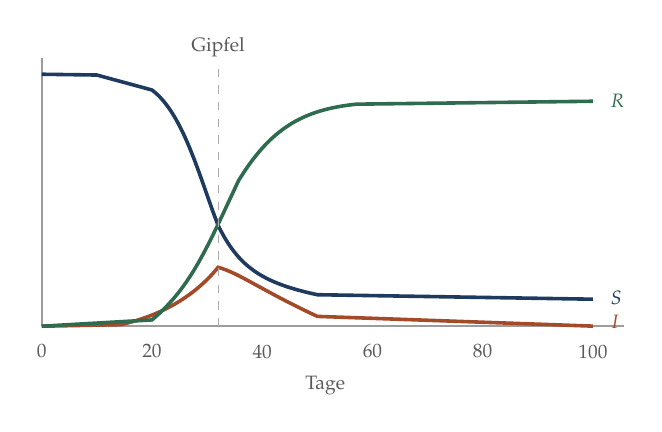
\begin{tikzpicture}[scale=1.0]
\draw[grau!60, line width=0.7pt] (0,0) -- (7.4,0);
\draw[grau!60, line width=0.7pt] (0,0) -- (0,3.4);
\foreach \x/\lab in {0/0, 1.4/20, 2.8/40, 4.2/60, 5.6/80, 7.0/100}
  \node[font=\scriptsize, color=grau] at (\x,-0.32) {\lab};
\node[font=\scriptsize, color=grau] at (3.6,-0.75) {Tage};
% S
\draw[tief, line width=1.3pt]
  (0,3.2) -- (0.7,3.19) -- (1.4,3.00) .. controls (1.8,2.7) and (2.0,1.9) .. (2.24,1.28)
  .. controls (2.5,0.75) and (2.8,0.55) .. (3.5,0.40) -- (7.0,0.343);
% I
\draw[akzent, line width=1.3pt]
  (0,0.0) -- (1.0,0.02) .. controls (1.6,0.15) and (2.0,0.45) .. (2.24,0.748)
  .. controls (2.5,0.68) and (2.8,0.45) .. (3.5,0.125) -- (7.0,0.001);
% R
\draw[gruen, line width=1.3pt]
  (0,0.0) -- (1.4,0.08) .. controls (1.9,0.5) and (2.1,1.0) .. (2.5,1.85)
  .. controls (2.9,2.5) and (3.3,2.75) .. (4.0,2.82) -- (7.0,2.857);
\draw[grau!50, dashed] (2.24,0) -- (2.24,3.3);
\node[font=\scriptsize, color=grau] at (2.24,3.55) {Gipfel};
\node[font=\scriptsize, color=tief, anchor=west] at (7.1,0.36) {$S$};
\node[font=\scriptsize, color=akzent, anchor=west] at (7.1,0.05) {$I$};
\node[font=\scriptsize, color=gruen, anchor=west] at (7.1,2.86) {$R$};
\end{tikzpicture}
\end{center}

\begin{center}
\begin{minipage}{0.88\textwidth}
\kursiv{Beachten Sie die Tage $20$ bis $30$: Der Anteil der Kranken steigt von $3{,}6$ auf $22{,}1$ Prozent --- in zehn Tagen mehr als das Sechsfache. Das ist die Eigenart exponentiellen Wachstums, das lange unauffällig bleibt und dann binnen weniger Verdopplungszeiten alles überrollt.}
\end{minipage}
\end{center}
\end{merksatz}

\section{Der Bruchfall}

\begin{warnung}
\boxtitelr{Die sechs Annahmen, einzeln geprüft}
\begin{center}
{\small
\renewcommand{\arraystretch}{1.5}
\begin{tabular}{@{}P{2.2cm}P{3.0cm}P{3.0cm}@{}}
\toprule
\textbf{Annahme} & \textbf{Verletzung} & \textbf{Folge}\\
\midrule
Durch\-mischung & Kontakte sind räumlich und sozial gebündelt & \textcolor{akzent}{Endgröße deutlich überschätzt}\\
Feste Zahl & Geburten, Zuzug & bei kurzen Epidemien unkritisch\\
Dauerhafter Schutz & Immunität lässt nach & wiederkehrende Wellen\\
Keine Inkubation & meist Tage & Gipfel später, Höhe kaum betroffen\\
Alle gleich & sehr verschieden & \textcolor{akzent}{Schwelle sinkt}\\
Massen\-wirkung & Verhalten ändert sich & \textcolor{akzent}{$\beta$ ist keine Konstante}\\
\bottomrule
\end{tabular}}
\end{center}

\schritt{Zur fünften Zeile --- die wichtigste Abweichung}
Streuen Ansteckbarkeit und Kontaktzahl stark, so erkranken die Kontaktfreudigsten zuerst. Die verbleibende Bevölkerung ist danach weniger gefährdet, als ihr Anteil vermuten lässt.

\begin{center}
\begin{minipage}{0.9\textwidth}
\textbf{Die Herdenschwelle liegt dann unter $1-1/\Rnull$, und die Endgröße unter dem berechneten Wert.}
\end{minipage}
\end{center}

\begin{center}
\begin{minipage}{0.88\textwidth}
\kursiv{Wie stark, hängt von der Streuung ab und ist schwer zu beziffern. Modelle mit starker Heterogenität liefern Schwellen, die deutlich unter der einfachen Formel liegen. Das ist ein Grund, warum die einfache Formel die Endgröße \kursiv{überschätzt} --- und kein Grund, sich darauf zu verlassen, denn die Streuung ist unbekannt.}
\end{minipage}
\end{center}

\schritt{Zur sechsten Zeile}
$\beta$ hängt vom Verhalten ab. Sobald über eine Epidemie berichtet wird, ändert es sich --- Menschen meiden Kontakte, waschen Hände, bleiben zu Hause.

\begin{center}
\begin{minipage}{0.9\textwidth}
\textbf{Das Modell beschreibt eine Bevölkerung, die nicht merkt, was geschieht.}
\end{minipage}
\end{center}

\begin{center}
\begin{minipage}{0.88\textwidth}
\kursiv{Das ist die grundlegendste Einschränkung, und keine Verfeinerung der Gleichungen behebt sie: Ein Modell, dessen Vorhersage das Verhalten ändert, sagt nicht mehr das vorher, was ohne es geschehen wäre. Kapitel~15 kommt auf dieses Eigenartige zurück.}
\end{minipage}
\end{center}
\end{warnung}

\begin{warnung}
\boxtitelr{Und die Empfindlichkeit gegenüber $\Rnull$}
\begin{center}
\renewcommand{\arraystretch}{1.48}
\begin{tabular}{@{}P{1.8cm}P{2.2cm}P{2.4cm}@{}}
\toprule
$\Rnull$ & \textbf{Endgröße} & \textbf{Gipfel}\\
\midrule
$2{,}0$ & $79{,}7\,\%$ & $15{,}3\,\%$\\
$2{,}5$ & $89{,}3\,\%$ & $23{,}3\,\%$\\
$3{,}0$ & $94{,}0\,\%$ & $30{,}0\,\%$\\
\bottomrule
\end{tabular}
\end{center}

Eine Unsicherheit von $\pm 20\,\%$ in $\Rnull$ führt zu einem Gipfel zwischen $15$ und $30$ Prozent --- einer Verdopplung.

\begin{center}
\begin{minipage}{0.88\textwidth}
\kursiv{Das ist die Warnung aus dem Vorwort in Zahlen: Genauigkeit ist nicht Richtigkeit. Wer eine Gipfelhöhe von \enquote{$23{,}3$ Prozent} berichtet, gibt eine Genauigkeit vor, die in der Eingangsgröße nicht steckt. Man berichtet Bänder.}
\end{minipage}
\end{center}
\end{warnung}

\section{Übungsaufgaben}

\begin{aufgabe}
\boxtitel{Aufgabe 7.1 --- $\Rnull$ aus Frühdaten schätzen}
In den ersten Tagen eines Ausbruchs verdoppeln sich die Fallzahlen alle $3{,}5$ Tage. Die mittlere Ansteckungsdauer beträgt $4$ Tage. Bestimmen Sie $\Rnull$, den Gipfel und die Endgröße.

\loesung
\schritt{Schritt 1 --- Die Wachstumsrate}
\[ r = \frac{\ln 2}{T_2} = \frac{0{,}6931}{3{,}5} = 0{,}1980\ \mathrm{d}^{-1} \]

\schritt{Schritt 2 --- Die Genesungsrate}
\[ \gamma = \frac{1}{4} = 0{,}25\ \mathrm{d}^{-1} \]

\schritt{Schritt 3 --- Die Reproduktionszahl}
In der Frühphase gilt $\dd I/\dd t = (\beta-\gamma)I$, also $r = \beta - \gamma$:
\[ \beta = r + \gamma = 0{,}1980 + 0{,}25 = 0{,}4480\ \mathrm{d}^{-1} \]
\[ \Rnull = \frac{\beta}{\gamma} = \frac{0{,}4480}{0{,}25} = 1{,}792 \]

\kursiv{Kurzformel:} $\Rnull = 1 + r/\gamma = 1 + 0{,}1980/0{,}25 = 1{,}792$. \checkmark

\schritt{Schritt 4 --- Der Gipfel}
\[ \ln 1{,}792 = 0{,}5834 \]
\[ \frac{I_{\max}}{N} = 1 - \frac{1+0{,}5834}{1{,}792} = 1 - \frac{1{,}5834}{1{,}792} = 1 - 0{,}8836 = 0{,}1164 \]

Etwa $11{,}6\,\%$ der Bevölkerung gleichzeitig krank.

\schritt{Schritt 5 --- Die Endgröße}
Wir lösen $s = e^{-1{,}792(1-s)}$:
\begin{center}
\renewcommand{\arraystretch}{1.38}
\begin{tabular}{@{}P{1.6cm}P{2.0cm}P{1.6cm}P{2.0cm}@{}}
\toprule
Schritt & $s$ & Schritt & $s$\\
\midrule
$0$ & $0{,}500$ & $10$ & $0{,}2748$\\
$2$ & $0{,}3305$ & $20$ & $0{,}2739$\\
$5$ & $0{,}2796$ & $\infty$ & $\mathbf{0{,}2739}$\\
\bottomrule
\end{tabular}
\end{center}
\[ \text{Befallsrate} = 1 - 0{,}2739 = 72{,}6\,\% \]

\schritt{Schritt 6 --- Die Probe}
\[ e^{-1{,}792 \cdot 0{,}7261} = e^{-1{,}3012} = 0{,}2722 \approx 0{,}274 \quad \checkmark \]

\schritt{Schritt 7 --- Die Empfindlichkeit prüfen}
Die Ansteckungsdauer ist meist unsicher. Wäre sie $5$ statt $4$ Tage:
\[ \gamma = 0{,}2, \quad \Rnull = 1 + \frac{0{,}198}{0{,}2} = 1{,}990 \]
\begin{center}
\renewcommand{\arraystretch}{1.48}
\begin{tabular}{@{}P{2.6cm}P{2.2cm}P{2.2cm}@{}}
\toprule
\textbf{Dauer} & $\Rnull$ & \textbf{Endgröße}\\
\midrule
$4$ Tage & $1{,}79$ & $72{,}6\,\%$\\
$5$ Tage & $1{,}99$ & $79{,}5\,\%$\\
\bottomrule
\end{tabular}
\end{center}

\begin{center}
\begin{minipage}{0.86\textwidth}
\kursiv{Ein Tag Unterschied in einer schwer messbaren Größe verändert die vorhergesagte Endgröße um sieben Prozentpunkte. Die Verdopplungszeit ist gut messbar, die Ansteckungsdauer nicht --- und $\Rnull$ hängt von beiden ab.}
\end{minipage}
\end{center}
\end{aufgabe}

\begin{aufgabe}
\boxtitel{Aufgabe 7.2 --- Den Gipfel senken}
Durch Maßnahmen wird $\beta$ in Neustadt von $0{,}5$ auf $0{,}3$ gesenkt. Wie ändern sich Schwelle, Gipfel und Endgröße?

\loesung
\schritt{Schritt 1 --- Die neue Reproduktionszahl}
\[ \Rnull = \frac{0{,}3}{0{,}2} = 1{,}5 \]

\schritt{Schritt 2 --- Der Gipfel}
\[ \ln 1{,}5 = 0{,}4055 \]
\[ \frac{I_{\max}}{N} = 1 - \frac{1{,}4055}{1{,}5} = 1 - 0{,}9370 = 0{,}0630 \]
\[ I_{\max} = 6\,300 \]

\schritt{Schritt 3 --- Die Endgröße}
$s = e^{-1{,}5(1-s)}$ liefert nach Iteration $s_\infty = 0{,}4172$, also eine Befallsrate von $58{,}3\,\%$.

\schritt{Schritt 4 --- Der Vergleich}
\begin{center}
{\small
\renewcommand{\arraystretch}{1.48}
\begin{tabular}{@{}P{2.6cm}P{1.8cm}P{1.8cm}P{1.8cm}@{}}
\toprule
& $\Rnull = 2{,}5$ & $\Rnull = 1{,}5$ & \textbf{Änderung}\\
\midrule
Schwelle & $60{,}0\,\%$ & $33{,}3\,\%$ & \\
Gipfel & $23\,350$ & $\mathbf{6\,300}$ & $-73\,\%$\\
Endgröße & $89\,300$ & $58\,300$ & $-35\,\%$\\
Wachstumsrate & $0{,}30$ & $0{,}10$ & $-67\,\%$\\
Verdopplungs\-zeit & $2{,}3$ d & $6{,}9$ d & $\times 3$\\
\bottomrule
\end{tabular}}
\end{center}

\schritt{Schritt 5 --- Die Deutung}
\begin{center}
\begin{minipage}{0.9\textwidth}
\textbf{Eine Senkung von $\beta$ um $40\,\%$ senkt den Gipfel um $73\,\%$ --- fast doppelt so stark.}
\end{minipage}
\end{center}

Der Grund ist die Nichtlinearität: Der Gipfel hängt über $\ln\Rnull/\Rnull$ von der Reproduktionszahl ab, nicht linear.

\begin{center}
\begin{minipage}{0.88\textwidth}
\kursiv{Das ist das rechnerische Argument für Maßnahmen zur Gipfelsenkung: Eine mäßige Verringerung der Kontakte wirkt auf den gleichzeitigen Krankenstand überproportional. Die Endgröße sinkt weit weniger --- sie wird vor allem \kursiv{verschoben}, nicht vermieden.}
\end{minipage}
\end{center}

\schritt{Schritt 6 --- Der Preis}
Die Verdopplungszeit verdreifacht sich, die Epidemie dauert entsprechend länger. Ein flacherer Gipfel bedeutet stets eine längere Epidemie --- die Fläche unter der Kurve entspricht der Endgröße und sinkt nur um ein Drittel.
\end{aufgabe}

\begin{aufgabe}
\boxtitel{Aufgabe 7.3 --- Die Formel für die Endgröße prüfen}
Zeigen Sie, dass die Gleichung $s = e^{-\Rnull(1-s)}$ für $\Rnull > 1$ genau zwei Lösungen in $[0,1]$ hat, und dass $s = 1$ stets eine davon ist.

\loesung
\schritt{Schritt 1 --- Die triviale Lösung}
Für $s = 1$:
\[ e^{-\Rnull(1-1)} = e^{0} = 1 = s . \quad \checkmark \]

\kursiv{Bedeutung:} Niemand erkrankt. Das ist die Lösung für den Fall, dass die Epidemie gar nicht beginnt.

\schritt{Schritt 2 --- Die Gleichung umformen}
Wir setzen
\[ h(s) = e^{-\Rnull(1-s)} - s \]
und suchen die Nullstellen von $h$ in $[0,1]$.

\schritt{Schritt 3 --- Die Randwerte}
\[ h(0) = e^{-\Rnull} - 0 = e^{-\Rnull} > 0 \]
\[ h(1) = 1 - 1 = 0 \]

\schritt{Schritt 4 --- Die Ableitung}
\[ h'(s) = \Rnull\,e^{-\Rnull(1-s)} - 1 \]
\[ h'(1) = \Rnull - 1 \]

\begin{center}
\begin{minipage}{0.9\textwidth}
\textbf{Für $\Rnull > 1$ ist $h'(1) > 0$: Die Funktion \kursiv{steigt} bei $s=1$.} Also war sie kurz vorher negativ.
\end{minipage}
\end{center}

\schritt{Schritt 5 --- Der Zwischenwertsatz}
$h$ ist stetig, $h(0) > 0$ und $h(s) < 0$ für $s$ knapp unter $1$. Also hat $h$ dazwischen eine Nullstelle.

\begin{center}
\begin{minipage}{0.88\textwidth}
\kursiv{Das ist die gesuchte Lösung: der Anteil, der bei einer tatsächlich ablaufenden Epidemie verschont bleibt.}
\end{minipage}
\end{center}

\schritt{Schritt 6 --- Dass es nur eine weitere gibt}
\[ h''(s) = \Rnull^2\,e^{-\Rnull(1-s)} > 0 \]
$h$ ist also überall streng konvex --- nach oben gekrümmt. Eine streng konvexe Funktion hat höchstens zwei Nullstellen.

Zusammen mit Schritt 5: \textbf{genau zwei.} $\blacksquare$

\schritt{Schritt 7 --- Der Fall $\Rnull < 1$}
Dann ist $h'(1) < 0$, die Funktion \kursiv{fällt} bei $s=1$. Zusammen mit $h(0)>0$ und der Konvexität folgt, dass $h$ auf $[0,1)$ keine Nullstelle hat.

\begin{center}
\begin{minipage}{0.9\textwidth}
\textbf{Für $\Rnull < 1$ bleibt nur $s_\infty = 1$: keine Epidemie.}
\end{minipage}
\end{center}

\schritt{Schritt 8 --- Die Einordnung}
\begin{center}
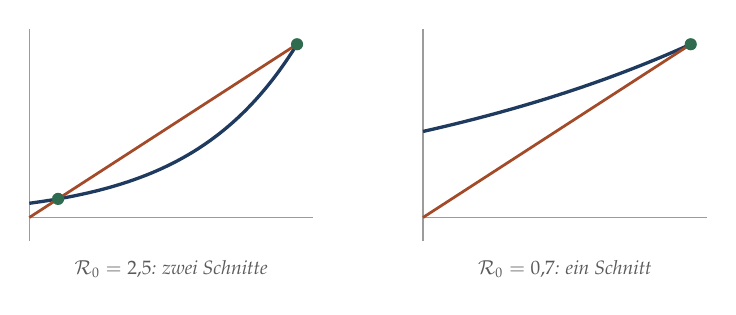
\begin{tikzpicture}[scale=1.0]
\begin{scope}
\draw[grau!60, line width=0.6pt] (0,0) -- (3.6,0);
\draw[grau!60, line width=0.6pt] (0,-0.3) -- (0,2.4);
\draw[tief, line width=1.2pt, smooth, samples=60, domain=0:3.4]
  plot (\x, {2.2*exp(-2.5*(1-\x/3.4))});
\draw[akzent, line width=1.0pt] (0,0) -- (3.4,2.2);
\fill[gruen] (0.365,0.236) circle (2.2pt);
\fill[gruen] (3.4,2.2) circle (2.2pt);
\node[font=\scriptsize\itshape, color=grau] at (1.8,-0.65) {$\Rnull = 2{,}5$: zwei Schnitte};
\end{scope}
\begin{scope}[xshift=5.0cm]
\draw[grau!60, line width=0.6pt] (0,0) -- (3.6,0);
\draw[grau!60, line width=0.6pt] (0,-0.3) -- (0,2.4);
\draw[tief, line width=1.2pt, smooth, samples=60, domain=0:3.4]
  plot (\x, {2.2*exp(-0.7*(1-\x/3.4))});
\draw[akzent, line width=1.0pt] (0,0) -- (3.4,2.2);
\fill[gruen] (3.4,2.2) circle (2.2pt);
\node[font=\scriptsize\itshape, color=grau] at (1.8,-0.65) {$\Rnull = 0{,}7$: ein Schnitt};
\end{scope}
\end{tikzpicture}
\end{center}

\begin{center}
\begin{minipage}{0.86\textwidth}
\kursiv{Der Schwellenwert $\Rnull = 1$ ist damit eine \Begriff{transkritische Bifurkation} im Sinne von Kapitel~6: Bei ihrem Durchschreiten wandert eine zweite Lösung aus dem Bereich $s>1$ herein und wird zur sinnvollen. Die gesamte Epidemiologie hängt an dieser einen Schwelle.}
\end{minipage}
\end{center}
\end{aufgabe}

\begin{geschichte}
\boxtitelg{Ein Arzt, ein Chemiker und ein Satz, der übersehen wurde}
\Person{William Kermack} (1898--1970), Chemiker, und \Person{Anderson McKendrick} (1876--1943), Militärarzt im indischen Sanitätsdienst, veröffentlichten 1927 in den \kursiv{Proceedings of the Royal Society} die Arbeit, die dieses Kapitel behandelt.

Sie enthält das Modell, den Schwellensatz und die Endgrößengleichung --- alles, was hier steht.

\begin{center}
\begin{minipage}{0.9\textwidth}
\kursiv{Die Arbeit wurde jahrzehntelang kaum beachtet. Erst in den 1970er Jahren, mit dem Aufkommen der mathematischen Epidemiologie als eigenem Fach, wurde sie zum meistzitierten Aufsatz des Gebiets. Der Schwellensatz gilt heute als eines der wichtigsten Ergebnisse der theoretischen Biologie überhaupt.}
\end{minipage}
\end{center}

\schritt{Kermacks Unfall}
1924, drei Jahre vor der Arbeit, erblindete Kermack bei einem Laborunfall durch eine Laugenexplosion vollständig. Er war sechsundzwanzig.

\begin{center}
\begin{minipage}{0.9\textwidth}
\kursiv{Er arbeitete weitere fünfundvierzig Jahre wissenschaftlich --- Kollegen lasen ihm vor, und er rechnete im Kopf. Zeitgenossen berichteten, seine Fähigkeit, lange Herleitungen ohne Papier zu führen, habe sich nach der Erblindung noch gesteigert. Die Arbeit von 1927 entstand vollständig auf diese Weise.}
\end{minipage}
\end{center}

\schritt{Der Vorläufer}
\Person{Ronald Ross} (1857--1932), Nobelpreisträger für die Entdeckung der Malariaübertragung durch Stechmücken, hatte bereits ab 1911 ähnliche Gleichungen aufgestellt.

\begin{center}
\begin{minipage}{0.9\textwidth}
\kursiv{Ross zog daraus eine praktisch folgenreiche Schlussfolgerung: Man muss die Mücken nicht ausrotten, um die Malaria auszurotten --- es genügt, ihre Zahl unter eine Schwelle zu drücken. Diese Einsicht war damals umstritten und ist die früheste Form des Schwellensatzes.}
\end{minipage}
\end{center}
\end{geschichte}

\begin{forschung}
\boxtitelp{Wo das SIR-Modell heute steht}
\begin{center}
{\small
\renewcommand{\arraystretch}{1.45}
\begin{tabular}{@{}P{2.8cm}P{5.4cm}@{}}
\toprule
\textbf{Als Grundbaustein} & Praktisch jedes Epidemiemodell ist eine Erweiterung: SEIR mit Inkubation, SIRS mit nachlassender Immunität, Altersgruppen, räumliche Struktur.\\
\textbf{$\Rnull$ als Berichtsgröße} & Hat sich weit über die Fachwelt hinaus verbreitet --- mit allen Missverständnissen, die das mit sich bringt.\\
\textbf{Netzwerk\-modelle} & Kontakte als Graph statt als Durchmischung. Kapitel~9.\\
\bottomrule
\end{tabular}}
\end{center}

\schritt{Was an $\Rnull$ regelmäßig missverstanden wird}
\begin{center}
{\small
\renewcommand{\arraystretch}{1.48}
\begin{tabular}{@{}P{3.0cm}P{5.2cm}@{}}
\toprule
\textcolor{akzent}{\enquote{Eine Eigenschaft des Erregers}} & Nein --- $\beta$ hängt vom Verhalten und von der Bevölkerungsdichte ab. Derselbe Erreger hat in verschiedenen Gesellschaften verschiedene $\Rnull$.\\
\textcolor{akzent}{\enquote{Eine feste Zahl}} & Nein --- $\Rnull$ wird geschätzt, mit erheblicher Unsicherheit, und die Schätzung hängt vom Modell ab.\\
\textcolor{akzent}{\enquote{$\Rnull<1$ heißt sicher}} & Nein --- es heißt, dass die Epidemie im Mittel abklingt. Einzelne Ausbrüche bleiben möglich.\\
\bottomrule
\end{tabular}}
\end{center}

\begin{center}
\begin{minipage}{0.88\textwidth}
\kursiv{Der erste Punkt ist der folgenreichste. $\Rnull$ ist keine Naturkonstante, sondern das Produkt aus Erregereigenschaften \kursiv{und} Gesellschaft. Genau deshalb lässt es sich durch Maßnahmen verändern --- was zugleich bedeutet, dass ein aus einer Bevölkerung geschätzter Wert nicht ohne Weiteres auf eine andere übertragbar ist.}
\end{minipage}
\end{center}

\schritt{Die Schätzung aus Daten}
Sie ist heikler, als die Formel $\Rnull = 1 + r/\gamma$ vermuten lässt. Sie setzt eine exponentiell verteilte Ansteckungsdauer voraus --- was selten zutrifft. Bei realistischeren Verteilungen ergibt sich aus derselben Wachstumsrate ein anderes $\Rnull$.

\begin{center}
\begin{minipage}{0.88\textwidth}
\kursiv{Die allgemeine Beziehung läuft über die Verteilung der Generationszeit. Bei stark gestreuter Generationszeit fällt $\Rnull$ für dieselbe beobachtete Wachstumsrate niedriger aus. Die in Umlauf gebrachten Zahlen hängen daher merklich davon ab, welches Modell ihnen zugrunde lag.}
\end{minipage}
\end{center}
\end{forschung}

\begin{merksatz}
\boxtitel{Was Sie jetzt können}
\begin{center}
\renewcommand{\arraystretch}{1.5}
\begin{tabular}{@{}P{3.0cm}P{5.6cm}@{}}
\toprule
\textbf{Definition 7.1} & drei Kammern, zwei Parameter\\
\textbf{Satz 7.2} & $\Rnull = \beta/\gamma$, Schwelle bei $1$\\
\textbf{Satz 7.3} & $I_{\max}/N = 1 - (1+\ln\Rnull)/\Rnull$\\
\textbf{Satz 7.4} & Endgröße aus $s = e^{-\Rnull(1-s)}$\\
\textbf{Überschwingen} & Endgröße weit über der Herdenschwelle\\
\bottomrule
\end{tabular}
\end{center}

\begin{center}
\begin{minipage}{0.88\textwidth}
\kursiv{Im nächsten Kapitel geht es um die Frage, wie viele geimpft werden müssen --- und warum die Antwort nicht \enquote{alle} lautet.}
\end{minipage}
\end{center}
\end{merksatz}

\chapter{Impfung und Schwellenwerte}

\section{Die Frage}

\begin{merksatz}
\boxtitel{Neustadt, ein Jahr später}
Gegen den Erreger steht nun ein Impfstoff zur Verfügung. Die Gesundheitsbehörde fragt:

\begin{center}
\begin{minipage}{0.9\textwidth}
\textbf{Wie viele Menschen müssen geimpft werden, damit sich der Erreger nicht mehr ausbreiten kann?}
\end{minipage}
\end{center}

Die Antwort lautet nicht \enquote{alle} --- und genau darin liegt der Wert des Modells.
\end{merksatz}

\begin{merksatz}
\boxtitel{Satz 8.1 --- die Herdenschwelle}
Wird ein Anteil $p$ der Bevölkerung vor Beginn immunisiert, so breitet sich der Erreger genau dann nicht aus, wenn
\[ p \;>\; p_c \;:=\; 1 - \frac{1}{\Rnull} . \]

\schritt{Beweis}
Geimpfte gehören von Anfang an zur Kammer $R$. Der Anteil der Empfänglichen beträgt also $S/N = 1-p$.

Nach Satz 7.2 breitet sich der Erreger aus, wenn
\[ \Rnull\cdot\frac{S}{N} > 1 \quad\Longleftrightarrow\quad \Rnull\,(1-p) > 1 . \]

Verneint man das:
\[ \Rnull\,(1-p) < 1 \quad\Longleftrightarrow\quad 1-p < \frac{1}{\Rnull} \quad\Longleftrightarrow\quad p > 1 - \frac{1}{\Rnull} . \qquad \blacksquare \]
\end{merksatz}

\begin{merksatz}
\boxtitel{Warum nicht alle geimpft werden müssen}
\begin{center}
\begin{minipage}{0.9\textwidth}
Eine ansteckende Person trifft im Mittel $\Rnull$ empfängliche Menschen --- \kursiv{wenn} alle empfänglich sind. Ist nur der Anteil $1-p$ empfänglich, so sind es nur $\Rnull(1-p)$.
\end{minipage}
\end{center}

Man muss also nicht jede Ansteckung verhindern, sondern nur so viele, dass jeder Ansteckende im Mittel weniger als einen neuen erzeugt.

\begin{center}
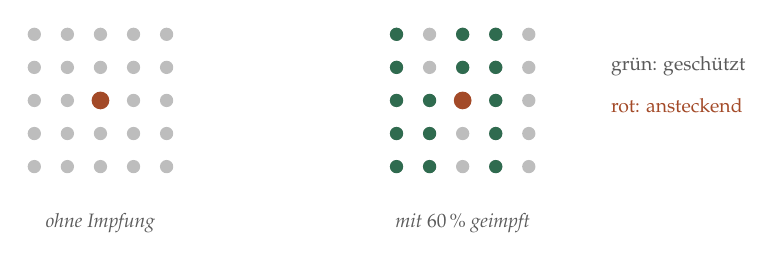
\begin{tikzpicture}[scale=1.0]
\begin{scope}
\foreach \i in {0,...,24} {
  \pgfmathsetmacro{\xx}{mod(\i,5)*0.42}
  \pgfmathsetmacro{\yy}{-floor(\i/5)*0.42}
  \fill[grau!40] (\xx,\yy) circle (2.4pt);
}
\fill[akzent] (0.84,-0.84) circle (3.2pt);
\node[font=\scriptsize\itshape, color=grau] at (0.84,-2.4) {ohne Impfung};
\end{scope}
\begin{scope}[xshift=4.6cm]
\foreach \i in {0,...,24} {
  \pgfmathsetmacro{\xx}{mod(\i,5)*0.42}
  \pgfmathsetmacro{\yy}{-floor(\i/5)*0.42}
  \fill[grau!40] (\xx,\yy) circle (2.4pt);
}
\foreach \i in {0,2,3,5,7,8,10,11,13,15,16,18,20,21,23} {
  \pgfmathsetmacro{\xx}{mod(\i,5)*0.42}
  \pgfmathsetmacro{\yy}{-floor(\i/5)*0.42}
  \fill[gruen] (\xx,\yy) circle (2.4pt);
}
\fill[akzent] (0.84,-0.84) circle (3.2pt);
\node[font=\scriptsize\itshape, color=grau] at (0.84,-2.4) {mit $60\,\%$ geimpft};
\end{scope}
\node[font=\scriptsize, color=grau, anchor=west] at (7.2,-0.4) {grün: geschützt};
\node[font=\scriptsize, color=akzent, anchor=west] at (7.2,-0.9) {rot: ansteckend};
\end{tikzpicture}
\end{center}
\end{merksatz}

\begin{merksatz}
\boxtitel{Die Schwellen für bekannte Erreger}
\begin{center}
{\small
\renewcommand{\arraystretch}{1.48}
\begin{tabular}{@{}P{2.6cm}P{2.2cm}P{2.6cm}@{}}
\toprule
\textbf{Erreger} & $\Rnull$ & \textbf{Schwelle $p_c$}\\
\midrule
Masern & $12$--$18$ & $92$--$94\,\%$\\
Keuchhusten & $12$--$17$ & $92$--$94\,\%$\\
Windpocken & $8$--$12$ & $88$--$92\,\%$\\
Röteln & $6$--$7$ & $83$--$86\,\%$\\
Pocken & $5$--$7$ & $80$--$86\,\%$\\
Mumps & $4$--$7$ & $75$--$86\,\%$\\
Neustädter Erreger & $2{,}5$ & $\mathbf{60\,\%}$\\
Grippe, saisonal & $1{,}2$--$1{,}4$ & $17$--$29\,\%$\\
\bottomrule
\end{tabular}}
\end{center}

\begin{center}
\begin{minipage}{0.88\textwidth}
\kursiv{Die Spannen sind echt: $\Rnull$ hängt von Bevölkerungsdichte, Altersaufbau und Verhalten ab und ist für denselben Erreger in verschiedenen Gesellschaften verschieden. Die Werte für Masern gehören zu den höchsten, die man kennt --- deshalb sind Masern der schwierigste Fall und zugleich der empfindlichste Anzeiger für Lücken im Impfschutz.}
\end{minipage}
\end{center}

\schritt{Die Antwort für Neustadt}
Bei $\Rnull = 2{,}5$ genügen $60\,\%$. Vierzig Prozent der Bevölkerung müssen nicht geimpft werden --- und sind trotzdem geschützt.
\end{merksatz}

\section{Unvollständiger Schutz}

\begin{warnung}
\boxtitelr{Kein Impfstoff wirkt bei allen}
Sei $\varepsilon$ der Anteil der Geimpften, bei denen der Impfschutz greift --- die \Begriff{Wirksamkeit}.

\schritt{Die neue Bedingung}
Der Anteil tatsächlich Geschützter beträgt $p\,\varepsilon$. Also
\[ p\,\varepsilon > 1 - \frac{1}{\Rnull} \quad\Longleftrightarrow\quad \boxed{\;p > \frac{1 - 1/\Rnull}{\varepsilon}\;} \]

\schritt{Die unbequeme Folgerung}
\begin{center}
\begin{minipage}{0.9\textwidth}
\textbf{Ist $\varepsilon < 1 - 1/\Rnull$, so lässt sich die Schwelle auch dann nicht erreichen, wenn jeder einzelne Mensch geimpft wird.}
\end{minipage}
\end{center}

Denn dann ist $p > 1$ verlangt, was unmöglich ist.

\schritt{Am Beispiel}
\begin{center}
{\small
\renewcommand{\arraystretch}{1.48}
\begin{tabular}{@{}P{1.8cm}P{1.6cm}P{2.2cm}P{2.4cm}@{}}
\toprule
$\Rnull$ & $p_c$ & $\varepsilon = 0{,}95$ & $\varepsilon = 0{,}60$\\
\midrule
$2{,}5$ & $60{,}0\,\%$ & $63{,}2\,\%$ & $100{,}0\,\%$\\
$6$ & $83{,}3\,\%$ & $87{,}7\,\%$ & \textcolor{akzent}{unmöglich}\\
$15$ & $93{,}3\,\%$ & $98{,}2\,\%$ & \textcolor{akzent}{unmöglich}\\
\bottomrule
\end{tabular}}
\end{center}

\kursiv{Rechnung für $\Rnull=15$, $\varepsilon=0{,}95$:}
\[ p > \frac{0{,}9333}{0{,}95} = 0{,}9824 \]

\begin{center}
\begin{minipage}{0.88\textwidth}
\kursiv{Bei Masern muss also praktisch jeder geimpft werden, obwohl der Impfstoff zu den wirksamsten gehört. Die zweite Impfung, die in vielen Ländern empfohlen wird, dient genau diesem Zweck: Sie hebt die Wirksamkeit von etwa $93\,\%$ auf über $97\,\%$ und macht die Schwelle dadurch überhaupt erst erreichbar.}
\end{minipage}
\end{center}
\end{warnung}

\section{Wenn die Schwelle nicht erreicht wird}

Der wichtigere Fall in der Praxis: Was nützt eine Impfquote \kursiv{unterhalb} der Schwelle?

\begin{merksatz}
\boxtitel{Die Endgröße bei teilweiser Impfung}
Wir wenden Satz 7.4 an, aber mit dem Ausgangsanteil $s_0 = 1-p$ statt $1$. Dieselbe Herleitung ergibt
\[ s_\infty = s_0\,e^{-\Rnull\,(s_0 - s_\infty)} . \]

\schritt{Für Neustadt, $\Rnull = 2{,}5$}
\begin{center}
{\small
\renewcommand{\arraystretch}{1.48}
\begin{tabular}{@{}P{1.4cm}P{1.6cm}P{2.2cm}P{2.6cm}@{}}
\toprule
$p$ & $s_0$ & \textbf{Erkrankte} & \textbf{davon bei den Ungeimpften}\\
\midrule
$0$ & $1{,}00$ & $89{,}3\,\%$ & $89{,}3\,\%$\\
$0{,}10$ & $0{,}90$ & $76{,}8\,\%$ & $85{,}3\,\%$\\
$0{,}20$ & $0{,}80$ & $63{,}7\,\%$ & $79{,}7\,\%$\\
$0{,}30$ & $0{,}70$ & $49{,}9\,\%$ & $71{,}3\,\%$\\
$0{,}40$ & $0{,}60$ & $35{,}0\,\%$ & $58{,}3\,\%$\\
$0{,}50$ & $0{,}50$ & $18{,}6\,\%$ & $37{,}1\,\%$\\
$0{,}55$ & $0{,}45$ & $9{,}6\,\%$ & $21{,}4\,\%$\\
$\mathbf{0{,}60}$ & $0{,}40$ & $\mathbf{0{,}2\,\%}$ & $0{,}4\,\%$\\
\bottomrule
\end{tabular}}
\end{center}

\schritt{Die Deutung}
\begin{center}
\begin{minipage}{0.9\textwidth}
\textbf{Jede Impfung nützt --- und zwar überproportional.} Zehn Prozent Impfquote senken die Zahl der Erkrankten um $12{,}5$ Prozentpunkte, nicht um zehn.
\end{minipage}
\end{center}

\schritt{Der indirekte Schutz}
Die rechte Spalte zeigt den Anteil der \kursiv{Ungeimpften}, die erkranken. Er fällt von $89{,}3$ auf $21{,}4$ Prozent --- ohne dass diese Menschen etwas getan hätten.

\begin{center}
\begin{minipage}{0.88\textwidth}
\kursiv{Das ist der \Begriff{indirekte Schutz}, und er ist der eigentliche Gegenstand dieses Kapitels. Eine Impfung nützt nicht nur der geimpften Person; sie nimmt den Erreger aus dem Umlauf und schützt dadurch auch diejenigen, die nicht geimpft werden können --- Säuglinge, Menschen mit geschwächtem Abwehrsystem, Personen mit Gegenanzeigen.}
\end{minipage}
\end{center}

\schritt{Die Nichtlinearität am Rand}
Von $p = 0{,}55$ auf $p = 0{,}60$ --- fünf Prozentpunkte --- fällt die Erkranktenzahl von $9{,}6$ auf $0{,}2$ Prozent.

\begin{center}
\begin{minipage}{0.9\textwidth}
\textbf{Die letzten Prozentpunkte vor der Schwelle bewirken am meisten.} Genau dort ist die Impfbereitschaft erfahrungsgemäß am schwersten zu erhöhen.
\end{minipage}
\end{center}
\end{merksatz}

\section{Die Altersverschiebung}

Nun ein Ergebnis, das der Anschauung zuwiderläuft und praktisch bedeutsam ist.

\begin{merksatz}
\boxtitel{Das Modell mit Nachwuchs}
Für Erreger, die über Jahrzehnte umlaufen, muss man Geburten berücksichtigen:
\[ \frac{\dd S}{\dd t} = \mu N - \beta\frac{SI}{N} - \mu S, \qquad
\frac{\dd I}{\dd t} = \beta\frac{SI}{N} - \gamma I - \mu I \]
mit der Geburts- und Sterberate $\mu = 1/L$, wobei $L$ die mittlere Lebensdauer ist.

\schritt{Das endemische Gleichgewicht}
Aus $\dd I/\dd t = 0$ mit $I \neq 0$:
\[ \beta\frac{S}{N} = \gamma + \mu \quad\Longrightarrow\quad \frac{S^{*}}{N} = \frac{\gamma+\mu}{\beta} = \frac{1}{\Rnull} \]
mit $\Rnull = \beta/(\gamma+\mu)$.

\begin{center}
\begin{minipage}{0.9\textwidth}
\textbf{Im Dauerzustand ist genau der Anteil $1/\Rnull$ empfänglich.} Die Krankheit reguliert sich selbst auf die Schwelle ein.
\end{minipage}
\end{center}

\begin{center}
\begin{minipage}{0.88\textwidth}
\kursiv{Das ist bemerkenswert: Der Anteil hängt nur von $\Rnull$ ab, nicht von der Geburtenrate. Und es liefert ein Verfahren zur Schätzung von $\Rnull$ aus Antikörperuntersuchungen --- misst man, welcher Anteil einer Bevölkerung noch nie Kontakt hatte, so kennt man $1/\Rnull$.}
\end{minipage}
\end{center}
\end{merksatz}

\begin{merksatz}
\boxtitel{Satz 8.2 --- das mittlere Erkrankungsalter}
Im endemischen Gleichgewicht beträgt das mittlere Alter bei Ansteckung näherungsweise
\[ A \;\approx\; \frac{L}{\Rnull - 1} . \]

\schritt{Begründung}
Eine empfängliche Person wird mit der Rate $\lambda = \beta I^{*}/N$ angesteckt. Die mittlere Wartezeit bis dahin ist $1/\lambda$ --- wie bei jedem exponentiellen Vorgang (Kapitel~1).

Aus dem Gleichgewicht der ersten Gleichung ergibt sich nach kurzer Rechnung $\lambda = \mu(\Rnull-1)$, also
\[ A = \frac{1}{\mu(\Rnull-1)} = \frac{L}{\Rnull-1} . \]

\schritt{Am Beispiel Masern}
$\Rnull = 15$, $L = 80$ Jahre:
\[ A = \frac{80}{14} = 5{,}7 \ \text{Jahre} \]

\begin{center}
\begin{minipage}{0.88\textwidth}
\kursiv{Das stimmt mit der Beobachtung überein: Vor Einführung der Impfung war Masern eine Krankheit des Vorschulalters. Je ansteckender ein Erreger, desto früher trifft er --- weil er praktisch jeden trifft, und zwar so bald wie möglich.}
\end{minipage}
\end{center}
\end{merksatz}

\begin{warnung}
\boxtitelr{Was die Impfung mit dem Erkrankungsalter macht}
Bei einer Impfquote $p$ unterhalb der Schwelle sinkt die effektive Reproduktionszahl auf $\Rnull(1-p)$. Also:
\[ A_p \approx \frac{L}{\Rnull(1-p) - 1} \]

\schritt{Für Röteln --- $\Rnull = 6$, $L = 75$ Jahre}
\begin{center}
{\small
\renewcommand{\arraystretch}{1.48}
\begin{tabular}{@{}P{1.6cm}P{2.0cm}P{2.6cm}@{}}
\toprule
$p$ & $\Rnull(1-p)$ & \textbf{mittleres Alter}\\
\midrule
$0$ & $6{,}00$ & $15{,}0$ Jahre\\
$0{,}30$ & $4{,}20$ & $23{,}4$\\
$0{,}50$ & $3{,}00$ & \textcolor{akzent}{$\mathbf{37{,}5}$}\\
$0{,}70$ & $1{,}80$ & $93{,}7$\\
$\mathbf{0{,}833}$ & $1{,}00$ & \textcolor{gruen}{Elimination}\\
\bottomrule
\end{tabular}}
\end{center}

\begin{center}
\begin{minipage}{0.9\textwidth}
\textbf{Eine Impfquote von $50\,\%$ verschiebt das mittlere Erkrankungsalter von $15$ auf $37$ Jahre.}
\end{minipage}
\end{center}

\schritt{Warum das gefährlich ist}
Röteln sind im Kindesalter harmlos. In der Schwangerschaft führen sie zu schweren Fehlbildungen beim Kind.

\begin{center}
\begin{minipage}{0.88\textwidth}
\kursiv{Eine unzureichende Impfquote kann daher die Zahl der schweren Fälle \kursiv{erhöhen}, obwohl die Gesamtzahl der Erkrankungen sinkt. Genau das geschah in Griechenland in den 1990er Jahren: Nach jahrelang mäßiger Impfquote kam es 1993 zu einem Rötelnausbruch mit ungewöhnlich vielen Erkrankungen im gebärfähigen Alter und in der Folge zur höchsten je dort verzeichneten Zahl angeborener Rötelnschäden.}
\end{minipage}
\end{center}

\schritt{Die Folgerung}
\begin{center}
\begin{minipage}{0.9\textwidth}
\textbf{Bei Erregern, deren Schwere mit dem Alter zunimmt, ist eine halbherzige Impfkampagne schlechter als keine.}
\end{minipage}
\end{center}

Das betrifft Röteln, Mumps, Windpocken, Hepatitis~A und Polio. Es betrifft \kursiv{nicht} Masern, deren Verlauf im Säuglingsalter am schwersten ist.

\begin{center}
\begin{minipage}{0.88\textwidth}
\kursiv{Die praktische Folgerung, die daraus gezogen wurde: Wer gegen Röteln impft, muss die Schwelle erreichen --- oder gezielt diejenigen impfen, für die die Krankheit gefährlich ist. Beides ist heute Bestandteil der Empfehlungen.}
\end{minipage}
\end{center}
\end{warnung}

\section{Der Bruchfall}

\begin{warnung}
\boxtitelr{Warum die Schwelle in der Wirklichkeit anders liegt}
\begin{center}
{\small
\renewcommand{\arraystretch}{1.5}
\begin{tabular}{@{}P{2.4cm}P{2.8cm}P{2.8cm}@{}}
\toprule
\textbf{Abweichung} & \textbf{Ursache} & \textbf{Folge}\\
\midrule
Heterogenität & Kontaktzahlen streuen & \textcolor{gruen}{Schwelle sinkt}\\
Bündelung & Ungeimpfte finden einander & \textcolor{akzent}{Schwelle steigt}\\
Nachlassender Schutz & Immunität schwindet & \textcolor{akzent}{Auffrischung nötig}\\
Einschleppung & keine geschlossene Bevölkerung & Ausbrüche bleiben möglich\\
\bottomrule
\end{tabular}}
\end{center}

\schritt{Die zweite Zeile ist die folgenreichste}
Das Modell setzt voraus, dass Geimpfte und Ungeimpfte gleichmäßig gemischt sind. Tatsächlich sammeln sich Impfgegner in bestimmten Schulen, Gemeinden und Regionen.

\begin{center}
\begin{minipage}{0.9\textwidth}
\textbf{Eine landesweite Impfquote von $95\,\%$ schützt nicht vor Ausbrüchen, wenn es einzelne Gemeinschaften mit $50\,\%$ gibt.} Dort ist die örtliche Reproduktionszahl über eins.
\end{minipage}
\end{center}

\begin{center}
\begin{minipage}{0.88\textwidth}
\kursiv{Alle größeren Masernausbrüche der letzten Jahrzehnte in Ländern mit hoher Durchimpfung folgten diesem Muster: Sie begannen in räumlich oder sozial abgegrenzten Gruppen mit niedriger Quote. Die Durchschnittszahl verdeckt das --- deshalb ist die \kursiv{Verteilung} der Impfquote wichtiger als ihr Mittelwert.}
\end{minipage}
\end{center}

\schritt{Zur ersten Zeile}
Streuen die Kontaktzahlen stark, so genügt es, die Kontaktfreudigsten zu impfen. Die Schwelle sinkt dann unter $1-1/\Rnull$.

\begin{center}
\begin{minipage}{0.88\textwidth}
\kursiv{Das ist die Grundlage gezielter Impfstrategien --- etwa der Riegelungsimpfung im Umfeld eines Falls, mit der die Pocken ausgerottet wurden. Sie wirkt, weil sie genau die Personen erreicht, über die die Übertragung läuft.}
\end{minipage}
\end{center}
\end{warnung}

\section{Übungsaufgaben}

\begin{aufgabe}
\boxtitel{Aufgabe 8.1 --- Schwelle mit unvollständiger Wirksamkeit}
Für einen Erreger mit $\Rnull = 8$ steht ein Impfstoff mit $\varepsilon = 0{,}90$ zur Verfügung. Welche Quote ist nötig? Was ändert sich bei $\varepsilon = 0{,}85$?

\loesung
\schritt{Schritt 1 --- Die Grundschwelle}
\[ p_c = 1 - \frac{1}{8} = 0{,}875 = 87{,}5\,\% \]

\schritt{Schritt 2 --- Mit $\varepsilon = 0{,}90$}
\[ p > \frac{0{,}875}{0{,}90} = 0{,}9722 = 97{,}2\,\% \]

\schritt{Schritt 3 --- Mit $\varepsilon = 0{,}85$}
\[ p > \frac{0{,}875}{0{,}85} = 1{,}0294 \]

Über eins --- \textbf{unmöglich.} Selbst bei vollständiger Durchimpfung bliebe die effektive Reproduktionszahl über eins.

\schritt{Schritt 4 --- Die Probe}
Bei $p=1$ und $\varepsilon = 0{,}85$ sind $85\,\%$ geschützt, $15\,\%$ empfänglich:
\[ \mathcal{R}_{\text{eff}} = 8 \cdot 0{,}15 = 1{,}20 > 1 \quad \textcolor{akzent}{\times} \]
Bei $\varepsilon = 0{,}90$: $\mathcal{R}_{\text{eff}} = 8 \cdot 0{,}10 = 0{,}80 < 1$ \checkmark

\schritt{Schritt 5 --- Die kritische Wirksamkeit}
Allgemein muss gelten $\varepsilon \ge p_c$, also hier $\varepsilon \ge 0{,}875$.

\begin{center}
\begin{minipage}{0.9\textwidth}
\textbf{Die Wirksamkeit muss mindestens so groß sein wie die Herdenschwelle.} Andernfalls ist Elimination durch Impfung allein ausgeschlossen.
\end{minipage}
\end{center}

\schritt{Schritt 6 --- Die Empfindlichkeit}
\begin{center}
\renewcommand{\arraystretch}{1.45}
\begin{tabular}{@{}P{2.0cm}P{2.4cm}P{2.4cm}@{}}
\toprule
$\varepsilon$ & \textbf{nötige Quote} & \\
\midrule
$1{,}00$ & $87{,}5\,\%$ & \\
$0{,}95$ & $92{,}1\,\%$ & \\
$0{,}90$ & $97{,}2\,\%$ & \\
$0{,}88$ & $99{,}4\,\%$ & \textcolor{akzent}{kaum erreichbar}\\
$0{,}875$ & $100{,}0\,\%$ & \textcolor{akzent}{Grenze}\\
\bottomrule
\end{tabular}
\end{center}

\begin{center}
\begin{minipage}{0.86\textwidth}
\kursiv{Fünf Prozentpunkte Wirksamkeit --- von $95$ auf $90$ --- erfordern fünf Prozentpunkte mehr Impfquote. Die letzten Zeilen zeigen, wie steil es danach wird: Nahe der kritischen Wirksamkeit wächst die nötige Quote über jede Grenze.}
\end{minipage}
\end{center}
\end{aufgabe}

\begin{aufgabe}
\boxtitel{Aufgabe 8.2 --- Die Altersverschiebung beziffern}
Für Mumps gilt $\Rnull = 5$ und $L = 78$ Jahre. Bestimmen Sie das mittlere Erkrankungsalter ohne Impfung und bei Quoten von $40$, $60$ und $75$ Prozent. Ab welcher Quote läge es über $20$ Jahren?

\loesung
\schritt{Schritt 1 --- Ohne Impfung}
\[ A = \frac{78}{5-1} = \frac{78}{4} = 19{,}5 \ \text{Jahre} \]

\begin{center}
\begin{minipage}{0.86\textwidth}
\kursiv{Schon ohne Impfung liegt das mittlere Alter bei knapp zwanzig Jahren. Mumps ist damit von vornherein ein Grenzfall --- die gefürchtete Hodenentzündung tritt vor allem nach der Pubertät auf.}
\end{minipage}
\end{center}

\schritt{Schritt 2 --- Die Schwelle}
\[ p_c = 1 - \frac{1}{5} = 0{,}80 = 80\,\% \]

\schritt{Schritt 3 --- Die Werte}
\begin{center}
\renewcommand{\arraystretch}{1.48}
\begin{tabular}{@{}P{1.6cm}P{2.2cm}P{2.6cm}@{}}
\toprule
$p$ & $\Rnull(1-p)$ & $A_p$\\
\midrule
$0$ & $5{,}00$ & $19{,}5$ J\\
$0{,}40$ & $3{,}00$ & $39{,}0$ J\\
$0{,}60$ & $2{,}00$ & $78{,}0$ J\\
$0{,}75$ & $1{,}25$ & $312{,}0$ J\\
$0{,}80$ & $1{,}00$ & \textcolor{gruen}{Elimination}\\
\bottomrule
\end{tabular}
\end{center}

\kursiv{Rechnung für $p=0{,}40$:} $A = 78/(3-1) = 39{,}0$.

\schritt{Schritt 4 --- Die Deutung der großen Werte}
Ein \enquote{mittleres Erkrankungsalter} von $312$ Jahren ist natürlich unsinnig. Die Zahl bedeutet: Die Ansteckungsrate ist so gering, dass die allermeisten Menschen \kursiv{nie} erkranken --- sie sterben vorher.

\begin{center}
\begin{minipage}{0.86\textwidth}
\kursiv{Die Formel gilt nur, solange $A$ klein gegen $L$ ist. Bei $A \ge L$ ist sie als Größenvergleich zu lesen, nicht als Vorhersage. Das ist eine Bruchstelle des Modells, die man kennen muss --- die Rechnung liefert weiter Zahlen, aber sie bedeuten etwas anderes.}
\end{minipage}
\end{center}

\schritt{Schritt 5 --- Ab welcher Quote über zwanzig Jahren}
\[ \frac{78}{5(1-p)-1} > 20 \]
\[ 5(1-p) - 1 < \frac{78}{20} = 3{,}9 \]
\[ 5(1-p) < 4{,}9 \quad\Longrightarrow\quad 1-p < 0{,}98 \quad\Longrightarrow\quad p > 0{,}02 \]

\schritt{Antwort}
\textbf{Ab zwei Prozent Impfquote.}

\begin{center}
\begin{minipage}{0.9\textwidth}
\textbf{Bei Mumps genügt schon eine minimale Impfquote, um das mittlere Erkrankungsalter über zwanzig Jahre zu schieben} --- weil es ohne Impfung bereits bei $19{,}5$ lag.
\end{minipage}
\end{center}

\begin{center}
\begin{minipage}{0.88\textwidth}
\kursiv{Das ist die schärfste Form des Arguments aus Abschnitt 8.4: Bei einem Erreger, dessen Erkrankungsalter ohnehin nahe der kritischen Grenze liegt, kippt jede unvollständige Impfung die Lage ins Ungünstige. Die einzige vertretbare Strategie ist dann, die Schwelle zu erreichen.}
\end{minipage}
\end{center}
\end{aufgabe}

\begin{aufgabe}
\boxtitel{Aufgabe 8.3 --- Wem nützt die Impfung?}
In Neustadt sind $50\,\%$ geimpft, $\Rnull = 2{,}5$. Von den Ungeimpften erkranken $37{,}1\,\%$. Vergleichen Sie den direkten und den indirekten Nutzen.

\loesung
\schritt{Schritt 1 --- Ohne jede Impfung}
Alle $100\,000$ sind empfänglich, $89\,300$ erkranken.

\schritt{Schritt 2 --- Mit $50\,\%$ Impfquote}
$50\,000$ Geimpfte erkranken nicht. Von den $50\,000$ Ungeimpften erkranken $37{,}1\,\%$:
\[ 0{,}371 \cdot 50\,000 = 18\,550 \]

\schritt{Schritt 3 --- Die Bilanz}
\begin{center}
\renewcommand{\arraystretch}{1.48}
\begin{tabular}{@{}P{3.0cm}P{2.2cm}P{2.4cm}@{}}
\toprule
& \textbf{ohne} & \textbf{mit $p=0{,}5$}\\
\midrule
Erkrankte gesamt & $89\,300$ & $18\,550$\\
Vermieden & --- & $\mathbf{70\,750}$\\
\bottomrule
\end{tabular}
\end{center}

\schritt{Schritt 4 --- Wer profitiert wovon}
\kursiv{Direkter Nutzen:} Die $50\,000$ Geimpften hätten ohne Impfung zu $89{,}3\,\%$ erkrankt, also
\[ 0{,}893 \cdot 50\,000 = 44\,650 \ \text{Fälle} . \]

\kursiv{Indirekter Nutzen:} Die $50\,000$ Ungeimpften hätten $44\,650$ Fälle gehabt, haben aber nur $18\,550$:
\[ 44\,650 - 18\,550 = 26\,100 \ \text{vermiedene Fälle} . \]

\begin{center}
\renewcommand{\arraystretch}{1.48}
\begin{tabular}{@{}P{3.0cm}P{2.2cm}P{2.4cm}@{}}
\toprule
\textbf{Nutzen} & \textbf{Fälle} & \textbf{Anteil}\\
\midrule
direkt (Geimpfte) & $44\,650$ & $63\,\%$\\
indirekt (Ungeimpfte) & $26\,100$ & $\mathbf{37\,\%}$\\
\midrule
Summe & $70\,750$ & $100\,\%$\\
\bottomrule
\end{tabular}
\end{center}

\schritt{Schritt 5 --- Die Deutung}
\begin{center}
\begin{minipage}{0.9\textwidth}
\textbf{Mehr als ein Drittel des Nutzens fällt bei Menschen an, die sich nicht haben impfen lassen.}
\end{minipage}
\end{center}

\schritt{Schritt 6 --- Je Geimpftem gerechnet}
\[ \frac{70\,750}{50\,000} = 1{,}42 \ \text{vermiedene Fälle je Impfung} \]

Eine Impfung verhindert im Mittel mehr als eine Erkrankung --- sie schützt die geimpfte Person \kursiv{und} einen halben weiteren Menschen.

\begin{center}
\begin{minipage}{0.88\textwidth}
\kursiv{Das ist der rechnerische Kern der Debatte um Impfpflichten. Die Entscheidung, sich nicht impfen zu lassen, betrifft nicht nur die entscheidende Person --- sie entzieht anderen einen Schutz, den diese nicht selbst herstellen können. Das Modell liefert dazu die Zahlen; die Abwägung liefert es nicht.}
\end{minipage}
\end{center}

\schritt{Schritt 7 --- Die Abhängigkeit von der Quote}
\begin{center}
\renewcommand{\arraystretch}{1.45}
\begin{tabular}{@{}P{1.8cm}P{2.6cm}P{2.6cm}@{}}
\toprule
$p$ & \textbf{vermieden je Impfung} & \\
\midrule
$0{,}10$ & $1{,}25$ & \\
$0{,}30$ & $1{,}31$ & \\
$0{,}50$ & $1{,}42$ & \\
$0{,}59$ & $1{,}51$ & \textcolor{gruen}{knapp unter der Schwelle}\\
\bottomrule
\end{tabular}
\end{center}

Je näher an der Schwelle, desto mehr bewirkt jede einzelne Impfung --- die Nichtlinearität aus Abschnitt 8.3 in einer anderen Gestalt.
\end{aufgabe}

\begin{geschichte}
\boxtitelg{Die einzige ausgerottete Krankheit des Menschen}
\Person{Edward Jenner} zeigte 1796, dass eine Infektion mit Kuhpocken gegen Menschenpocken schützt. Das Wort \kursiv{Vakzine} stammt vom lateinischen \kursiv{vacca} --- Kuh.

\begin{center}
\begin{minipage}{0.9\textwidth}
\kursiv{Jenner war nicht der Erste. Die Beobachtung, dass Melkerinnen keine Pocken bekamen, war unter Landärzten bekannt; der Bauer Benjamin Jesty hatte schon 1774 seine Familie geimpft. Jenners Verdienst war, es systematisch zu prüfen und zu veröffentlichen.}
\end{minipage}
\end{center}

\schritt{Die Ausrottung}
Die Weltgesundheitsorganisation beschloss 1967 ein weltweites Ausrottungsprogramm. Die Pocken hatten damals noch etwa zwei Millionen Todesfälle im Jahr zur Folge.

Der letzte natürlich erworbene Fall trat 1977 in Somalia auf; 1980 wurden die Pocken für ausgerottet erklärt.

\begin{center}
\begin{minipage}{0.9\textwidth}
\kursiv{Entscheidend war nicht die flächendeckende Impfung, sondern ein Strategiewechsel: Statt möglichst viele zu impfen, suchte man jeden Fall auf und impfte sein gesamtes Umfeld. Diese \Begriff{Riegelungsimpfung} erreichte die Ausrottung mit Quoten, die deutlich unter der Herdenschwelle lagen.}
\end{minipage}
\end{center}

\schritt{Warum das mathematisch funktioniert}
Die Schwellenformel setzt gleichmäßige Durchmischung voraus. Die Riegelungsimpfung nutzt das Gegenteil aus: Sie impft genau dort, wo das Ansteckungsgeschehen stattfindet.

\begin{center}
\begin{minipage}{0.9\textwidth}
\kursiv{Damit ist sie ein Beispiel dafür, dass eine Bruchstelle des Modells --- die verletzte Durchmischungsannahme --- sich auch \kursiv{nutzen} lässt. Vier Eigenschaften der Pocken machten es möglich: kein Tierreservoir, keine unbemerkten Verläufe, ein wirksamer und hitzestabiler Impfstoff, und ein Erreger ohne relevante Veränderlichkeit.}
\end{minipage}
\end{center}

\schritt{Warum es bei anderen nicht gelingt}
\begin{center}
{\small
\renewcommand{\arraystretch}{1.45}
\begin{tabular}{@{}P{2.2cm}P{2.6cm}P{3.2cm}@{}}
\toprule
\textbf{Erreger} & \textbf{Hindernis} & \\
\midrule
Polio & unbemerkte Verläufe & über $99\,\%$ ohne Lähmung\\
Masern & sehr hohes $\Rnull$ & Schwelle bei $94\,\%$\\
Grippe & Veränderlichkeit & jährlich neuer Impfstoff\\
Gelbfieber & Tierreservoir & Affen als Rückzugsort\\
\bottomrule
\end{tabular}}
\end{center}
\end{geschichte}

\begin{forschung}
\boxtitelp{Wohin sich die Impfmodellierung bewegt}
\begin{center}
{\small
\renewcommand{\arraystretch}{1.45}
\begin{tabular}{@{}P{2.8cm}P{5.4cm}@{}}
\toprule
\textbf{Alters\-strukturierte Modelle} & Kontaktmatrizen aus Befragungen; sie zeigen, dass Kinder untereinander weit mehr Kontakte haben als mit Erwachsenen.\\
\textbf{Räumliche Bündelung} & Modelle mit örtlich schwankender Impfquote; sie sagen Ausbrüche vorher, die Durchschnittsmodelle ausschließen.\\
\textbf{Verhaltens\-modelle} & Die Impfbereitschaft hängt von der wahrgenommenen Gefahr ab --- und die sinkt, wenn die Impfung wirkt.\\
\bottomrule
\end{tabular}}
\end{center}

\schritt{Die dritte Zeile}
Sie beschreibt eine Rückkopplung, die dem Modell dieses Kapitels fehlt: Eine erfolgreiche Impfkampagne lässt die Krankheit verschwinden --- und damit auch die Erinnerung an ihre Schwere.

\begin{center}
\begin{minipage}{0.88\textwidth}
\kursiv{Man kann daraus ein Modell bauen, in dem die Impfquote selbst eine Zustandsgröße ist. Solche Modelle zeigen regelmäßig Schwingungen: Die Quote steigt nach Ausbrüchen, sinkt in ruhigen Zeiten, bis ein neuer Ausbruch folgt. Das Muster entspricht dem, was man bei Masern in mehreren Ländern beobachtet hat --- und es ist wieder die verzögerte Rückkopplung aus Kapitel~3.}
\end{minipage}
\end{center}

\schritt{Die Kontaktmatrizen}
Groß angelegte Befragungen zum Kontaktverhalten haben die Modellierung verändert: Statt einer Durchmischungsannahme benutzt man gemessene Kontaktzahlen zwischen Altersgruppen.

\begin{center}
\begin{minipage}{0.88\textwidth}
\kursiv{Das Ergebnis ist eine Matrix mit starkem Übergewicht auf der Diagonale --- Menschen treffen überwiegend Gleichaltrige --- und einem Nebenband, das Eltern und Kinder verbindet. Aus ihr ergibt sich $\Rnull$ als größter Eigenwert, wieder mit dem Werkzeug aus Kapitel~6.}
\end{minipage}
\end{center}
\end{forschung}

\begin{merksatz}
\boxtitel{Was Sie jetzt können}
\begin{center}
\renewcommand{\arraystretch}{1.5}
\begin{tabular}{@{}P{3.4cm}P{5.2cm}@{}}
\toprule
\textbf{Satz 8.1} & Herdenschwelle $p_c = 1-1/\Rnull$\\
\textbf{Mit Wirksamkeit} & $p > p_c/\varepsilon$; unmöglich, falls $\varepsilon < p_c$\\
\textbf{Unterhalb der Schwelle} & jede Impfung nützt, zunehmend\\
\textbf{Satz 8.2} & $A \approx L/(\Rnull-1)$\\
\textbf{Alters\-verschiebung} & halbherziges Impfen kann schaden\\
\bottomrule
\end{tabular}
\end{center}

\begin{center}
\begin{minipage}{0.88\textwidth}
\kursiv{Im nächsten Kapitel geben wir die Durchmischungsannahme auf --- und stellen Kontakte als Netzwerk dar. Dabei zeigt sich, dass die Schwelle bei manchen Netzen überhaupt nicht existiert.}
\end{minipage}
\end{center}
\end{merksatz}

\chapter{Netzwerke und Heterogenität}

\section{Die Annahme, die nie stimmt}

Die Kapitel~7 und 8 setzten voraus, dass jeder jeden mit gleicher Wahrscheinlichkeit trifft. Das ist die erste der sechs Annahmen aus Abschnitt 7.1, und sie ist die falscheste.

\begin{merksatz}
\boxtitel{Was tatsächlich vorliegt}
\begin{center}
{\small
\renewcommand{\arraystretch}{1.5}
\begin{tabular}{@{}P{2.6cm}P{6.0cm}@{}}
\toprule
\textbf{Feste Partner} & Menschen treffen überwiegend dieselben Personen wieder --- Familie, Kollegen, Nachbarn.\\
\textbf{Sehr ungleiche Zahlen} & Manche haben drei enge Kontakte täglich, andere dreihundert.\\
\textbf{Gruppen} & Kontakte bilden Klumpen: Wer meine Freunde kennt, kennt oft auch einander.\\
\bottomrule
\end{tabular}}
\end{center}

\begin{center}
\begin{minipage}{0.9\textwidth}
Statt einer durchmischten Masse liegt ein \Begriff{Netzwerk} vor: Personen als Ecken, mögliche Übertragungswege als Kanten. Die Werkzeuge dafür stehen in Band 16.
\end{minipage}
\end{center}

\begin{center}
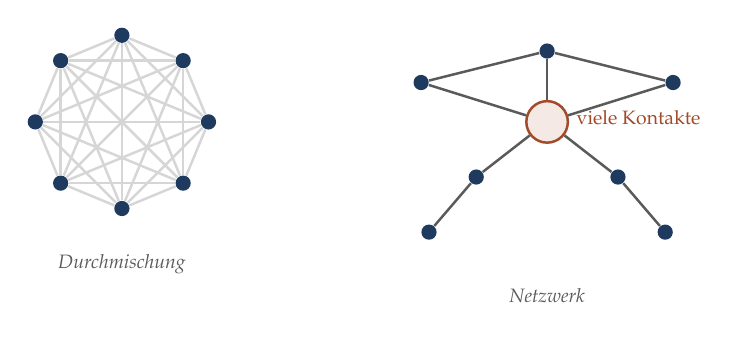
\begin{tikzpicture}[scale=1.0]
\begin{scope}
\foreach \i in {0,...,7} {
  \node[knoten] (h\i) at ({45*\i}:1.1) {};
}
\foreach \i in {0,...,7} \foreach \j in {0,...,7} {
  \ifnum\i<\j \draw[kante, grau!25] (h\i)--(h\j); \fi
}
\node[font=\scriptsize\itshape, color=grau] at (0,-1.8) {Durchmischung};
\end{scope}
\begin{scope}[xshift=5.4cm]
\node[knoten] (a) at (0,0.9) {};
\node[knotenr] (b) at (0,0) {};
\node[knoten] (c) at (-0.9,-0.7) {};
\node[knoten] (d) at (0.9,-0.7) {};
\node[knoten] (e) at (-1.6,0.5) {};
\node[knoten] (f) at (1.6,0.5) {};
\node[knoten] (g) at (-1.5,-1.4) {};
\node[knoten] (h) at (1.5,-1.4) {};
\draw[kante] (b)--(a); \draw[kante] (b)--(c); \draw[kante] (b)--(d);
\draw[kante] (b)--(e); \draw[kante] (b)--(f);
\draw[kante] (c)--(g); \draw[kante] (d)--(h);
\draw[kante] (a)--(e); \draw[kante] (a)--(f);
\node[font=\scriptsize\itshape, color=grau] at (0,-2.2) {Netzwerk};
\node[font=\scriptsize, color=akzent, anchor=west] at (0.25,0.05) {viele Kontakte};
\end{scope}
\end{tikzpicture}
\end{center}
\end{merksatz}

\begin{definition}
\boxtitelm{Definition 9.1 --- Gradverteilung}
Der \Begriff{Grad} $k$ einer Person ist die Zahl ihrer Kontakte. Die \Begriff{Gradverteilung} $p_k$ gibt an, welcher Anteil der Bevölkerung genau $k$ Kontakte hat.

Wir schreiben
\[ \langle k\rangle = \sum_k k\,p_k \qquad\text{und}\qquad \langle k^2\rangle = \sum_k k^2\,p_k \]
für den Mittelwert und den Mittelwert der Quadrate.
\end{definition}

\section{Das Freundschaftsparadoxon}

\begin{merksatz}
\boxtitel{Wen man erreicht, wenn man einer Kante folgt}
\begin{center}
\begin{minipage}{0.9\textwidth}
\textbf{Eine Person mit $k$ Kontakten ist über $k$ Kanten erreichbar. Folgt man einer zufällig gewählten Kante, so landet man bei kontaktreichen Personen mit entsprechend höherer Wahrscheinlichkeit.}
\end{minipage}
\end{center}

\schritt{Die Verteilung am Kantenende}
Die Wahrscheinlichkeit, über eine zufällige Kante bei einer Person vom Grad $k$ zu landen, ist proportional zu $k\,p_k$. Nach Normierung:
\[ q_k = \frac{k\,p_k}{\langle k\rangle} \]

\schritt{Der mittlere Grad dort}
\[ \sum_k k\,q_k = \sum_k k\cdot\frac{k\,p_k}{\langle k\rangle} = \frac{\langle k^2\rangle}{\langle k\rangle} \]

\begin{center}
\begin{minipage}{0.9\textwidth}
\textbf{Der Kontakt einer zufälligen Person hat im Mittel $\langle k^2\rangle/\langle k\rangle$ Kontakte --- und das ist stets mindestens so groß wie $\langle k\rangle$.}
\end{minipage}
\end{center}

\schritt{Der Nachweis}
Nach dem Verschiebungssatz (Band 17, Satz 2.11) ist
\[ \langle k^2\rangle - \langle k\rangle^2 = \operatorname{Var}(k) \ge 0 \quad\Longrightarrow\quad \frac{\langle k^2\rangle}{\langle k\rangle} \ge \langle k\rangle . \]
Gleichheit gilt nur, wenn alle denselben Grad haben.

\begin{center}
\begin{minipage}{0.88\textwidth}
\kursiv{Das ist das \Begriff{Freundschaftsparadoxon}: Die eigenen Freunde haben im Mittel mehr Freunde als man selbst. Es gilt für fast jede Person und ist kein psychologischer Effekt, sondern eine Folge der Auswahl --- kontaktreiche Menschen tauchen in mehr Freundeslisten auf.}
\end{minipage}
\end{center}
\end{merksatz}

\begin{merksatz}
\boxtitel{Satz 9.2 --- die Reproduktionszahl auf einem Netz}
Sei $T$ die Wahrscheinlichkeit, dass eine Übertragung entlang einer Kante stattfindet. Dann ist
\[ \Rnull \;=\; T\left(\frac{\langle k^2\rangle}{\langle k\rangle} - 1\right) . \]

\schritt{Begründung}
Eine angesteckte Person wurde über eine Kante erreicht. Sie hat im Mittel $\langle k^2\rangle/\langle k\rangle$ Kontakte, von denen einer die Quelle war --- also bleiben
\[ \frac{\langle k^2\rangle}{\langle k\rangle} - 1 \]
mögliche Empfänger. Über jede dieser Kanten überträgt sie mit Wahrscheinlichkeit $T$. $\blacksquare$

\schritt{Die Schwelle}
\[ \Rnull > 1 \quad\Longleftrightarrow\quad T > T_c := \frac{1}{\frac{\langle k^2\rangle}{\langle k\rangle} - 1} = \frac{\langle k\rangle}{\langle k^2\rangle - \langle k\rangle} \]
\end{merksatz}

\begin{merksatz}
\boxtitel{Zwei Netze mit demselben Durchschnitt}
\begin{center}
{\small
\renewcommand{\arraystretch}{1.5}
\begin{tabular}{@{}P{3.0cm}P{1.4cm}P{1.6cm}P{2.0cm}@{}}
\toprule
\textbf{Netz} & $\langle k\rangle$ & $\langle k^2\rangle$ & $T_c$\\
\midrule
alle $k=10$ & $10$ & $100$ & $0{,}1111$\\
$90\,\%$: $k=5$, $10\,\%$: $k=55$ & $10$ & $325$ & $0{,}0317$\\
$99\,\%$: $k=5$, $1\,\%$: $k=505$ & $10$ & $2575$ & $\mathbf{0{,}0039}$\\
\bottomrule
\end{tabular}}
\end{center}

\kursiv{Rechnung für die mittlere Zeile:}
\[ \langle k\rangle = 0{,}9\cdot5 + 0{,}1\cdot55 = 4{,}5+5{,}5 = 10 \]
\[ \langle k^2\rangle = 0{,}9\cdot25 + 0{,}1\cdot3025 = 22{,}5+302{,}5 = 325 \]
\[ \frac{\langle k^2\rangle}{\langle k\rangle} = 32{,}5, \qquad T_c = \frac{1}{31{,}5} = 0{,}0317 \]

\begin{center}
\begin{minipage}{0.9\textwidth}
\textbf{Alle drei Netze haben dieselbe mittlere Kontaktzahl. Die Ausbreitungsschwelle unterscheidet sich um den Faktor $28$.}
\end{minipage}
\end{center}

\begin{center}
\begin{minipage}{0.88\textwidth}
\kursiv{Damit ist die entscheidende Einsicht dieses Kapitels formuliert: \textbf{Nicht die mittlere Kontaktzahl bestimmt die Ausbreitung, sondern ihre Streuung.} Eine wenige Personen umfassende Gruppe mit sehr vielen Kontakten kann eine Epidemie tragen, die in einer gleichmäßigen Bevölkerung derselben Kontaktzahl erloschen wäre.}
\end{minipage}
\end{center}
\end{merksatz}

\begin{warnung}
\boxtitelr{Netze ohne Schwelle}
In vielen gemessenen Netzen folgt die Gradverteilung näherungsweise einem Potenzgesetz:
\[ p_k \sim k^{-\alpha} \qquad\text{mit}\qquad 2 < \alpha \le 3 . \]

\schritt{Was dann mit $\langle k^2\rangle$ geschieht}
\[ \langle k^2\rangle = \sum_k k^2\,p_k \sim \sum_k k^{2-\alpha} \]
Für $\alpha \le 3$ ist der Exponent $2-\alpha \ge -1$, und die Summe \kursiv{wächst über jede Grenze}, wenn das Netz groß wird.

\begin{center}
\begin{minipage}{0.9\textwidth}
\textbf{Dann ist $T_c = 0$: Es gibt keine Schwelle.} Jede noch so kleine Übertragungswahrscheinlichkeit genügt für eine Ausbreitung.
\end{minipage}
\end{center}

\begin{center}
\begin{minipage}{0.88\textwidth}
\kursiv{Dieses Ergebnis von Pastor-Satorras und Vespignani (2001) war eine Überraschung. Es erklärte, warum sich Rechnerviren in Netzen halten konnten, deren Ansteckungswahrscheinlichkeit weit unter jeder klassischen Schwelle lag --- und es hat die Netzwerkepidemiologie begründet.}
\end{minipage}
\end{center}

\schritt{Die Einschränkung}
Reale Netze sind endlich. Dann ist $\langle k^2\rangle$ endlich und die Schwelle nur \kursiv{sehr klein}, nicht null. Für praktische Zwecke läuft es auf dasselbe hinaus.

\begin{center}
\begin{minipage}{0.88\textwidth}
\kursiv{Ob menschliche Kontaktnetze wirklich einem Potenzgesetz folgen, ist umstritten. Bei Sexualkontakten deuten Befragungen darauf hin; bei Alltagskontakten spricht mehr für eine Verteilung mit endlichem, aber großem zweitem Moment. Die Folgerung bleibt in beiden Fällen dieselbe: Die Streuung zählt mehr als der Mittelwert.}
\end{minipage}
\end{center}
\end{warnung}

\section{Überstreuung und Superspreading}

\begin{merksatz}
\boxtitel{Nicht jeder steckt gleich viele an}
$\Rnull$ ist ein \kursiv{Mittelwert}. Die tatsächliche Zahl der Ansteckungen je Person schwankt erheblich.

\begin{center}
\begin{minipage}{0.9\textwidth}
Man beschreibt sie durch eine negative Binomialverteilung mit dem \Begriff{Überstreuungsparameter} $k$. Kleines $k$ bedeutet starke Streuung.
\end{minipage}
\end{center}

\begin{center}
{\small
\renewcommand{\arraystretch}{1.48}
\begin{tabular}{@{}P{1.6cm}P{2.8cm}P{3.4cm}@{}}
\toprule
$k$ & \textbf{Bedeutung} & \textbf{Beispiel}\\
\midrule
$\to\infty$ & Poisson, wenig Streuung & Modelle der Kapitel 7--8\\
$1$ & geometrisch & \\
$0{,}5$ & stark gestreut & \\
$\approx 0{,}16$ & sehr stark & SARS (2003)\\
$\approx 0{,}1$ & extrem & Masernausbrüche in Gruppen\\
\bottomrule
\end{tabular}}
\end{center}

\schritt{Wie ungleich die Übertragung verteilt ist}
\begin{center}
{\small
\renewcommand{\arraystretch}{1.48}
\begin{tabular}{@{}P{1.6cm}P{4.4cm}@{}}
\toprule
$k$ & \textbf{Anteil der Übertragungen durch die obersten $20\,\%$}\\
\midrule
$5{,}0$ & $43{,}8\,\%$\\
$1{,}0$ & $58{,}0\,\%$\\
$0{,}5$ & $69{,}2\,\%$\\
$0{,}16$ & $\mathbf{90{,}3\,\%}$\\
$0{,}1$ & $96{,}5\,\%$\\
\bottomrule
\end{tabular}}
\end{center}

\begin{center}
\begin{minipage}{0.88\textwidth}
\kursiv{Die vorletzte Zeile ist die berühmte Zwanzig-Achtzig-Regel: Bei $k \approx 0{,}16$ verursachen zwanzig Prozent der Fälle rund neunzig Prozent der Übertragungen. Der Rest steckt niemanden oder nur einen an.}
\end{minipage}
\end{center}
\end{merksatz}

\begin{merksatz}
\boxtitel{Satz 9.3 --- Wahrscheinlichkeit, dass ein Einzelfall folgenlos bleibt}
Wird ein einzelner Fall eingeschleppt, so erlischt die Kette mit Wahrscheinlichkeit $q$, wobei $q$ die kleinste Lösung von
\[ q = \left(1 + \frac{\Rnull}{k}(1-q)\right)^{-k} \]
in $[0,1]$ ist.

\schritt{Für $\Rnull = 2{,}5$}
\begin{center}
{\small
\renewcommand{\arraystretch}{1.48}
\begin{tabular}{@{}P{1.8cm}P{2.4cm}P{2.6cm}@{}}
\toprule
$k$ & \textbf{erlischt} & \textbf{Ausbruch}\\
\midrule
$\to\infty$ & $10{,}7\,\%$ & $89{,}3\,\%$\\
$5{,}0$ & $17{,}9\,\%$ & $82{,}1\,\%$\\
$1{,}0$ & $40{,}0\,\%$ & $60{,}0\,\%$\\
$0{,}5$ & $55{,}8\,\%$ & $44{,}2\,\%$\\
$0{,}16$ & $\mathbf{79{,}5\,\%}$ & $\mathbf{20{,}5\,\%}$\\
$0{,}1$ & $86{,}1\,\%$ & $13{,}9\,\%$\\
\bottomrule
\end{tabular}}
\end{center}

\begin{center}
\begin{minipage}{0.9\textwidth}
\textbf{Bei gleichem $\Rnull = 2{,}5$ erlischt eine Einschleppung mal in elf, mal in acht von zehn Fällen.} Der Unterschied liegt allein in der Streuung.
\end{minipage}
\end{center}

\begin{center}
\begin{minipage}{0.88\textwidth}
\kursiv{Bei starker Überstreuung sind die meisten Einschleppungen folgenlos --- und die wenigen, die nicht folgenlos bleiben, wachsen umso schneller. Das erklärt ein Muster, das bei SARS 2003 auffiel: lange Zeit nichts, dann plötzlich ein Ausbruch mit Dutzenden Fällen aus einer einzigen Quelle.}
\end{minipage}
\end{center}
\end{merksatz}

\begin{merksatz}
\boxtitel{Was daraus für Maßnahmen folgt}
\begin{center}
{\small
\renewcommand{\arraystretch}{1.52}
\begin{tabular}{@{}P{3.2cm}P{5.4cm}@{}}
\toprule
\textbf{Ausrottung ist leichter} & Weil die meisten Ketten von selbst erlöschen, genügen weniger Maßnahmen als bei gleichmäßiger Übertragung.\\
\textbf{Rückwärts\-verfolgung} & Sucht man von einem Fall aus \kursiv{rückwärts} nach der Quelle, so landet man mit hoher Wahrscheinlichkeit bei einem Superspreader --- und damit bei einem ganzen Bündel weiterer Fälle.\\
\textbf{Gelegenheiten statt Personen} & Superspreading hängt meist weniger an der Person als an der Gelegenheit: enge Räume, viele Menschen, lange Dauer, laute Umgebung.\\
\bottomrule
\end{tabular}}
\end{center}

\schritt{Warum die Rückwärtsverfolgung wirkt}
Das ist genau das Freundschaftsparadoxon aus Abschnitt 9.2, angewandt auf Ansteckungsketten: Ein zufällig gefundener Fall wurde mit erhöhter Wahrscheinlichkeit von jemandem angesteckt, der viele angesteckt hat.

\begin{center}
\begin{minipage}{0.88\textwidth}
\kursiv{Die übliche Kontaktverfolgung sucht vorwärts --- wen hat dieser Fall angesteckt? Die Rückwärtsverfolgung fragt zuerst: Wer hat ihn angesteckt? Und findet dadurch häufig ein ganzes Ereignis statt einzelner Kontakte. Modellrechnungen legen nahe, dass sie bei stark überstreuten Erregern zwei- bis dreimal so viele Fälle findet.}
\end{minipage}
\end{center}
\end{merksatz}

\section{Der Bruchfall}

\begin{warnung}
\boxtitelr{Was auch das Netzwerkmodell nicht leistet}
\begin{center}
{\small
\renewcommand{\arraystretch}{1.5}
\begin{tabular}{@{}P{2.6cm}P{6.0cm}@{}}
\toprule
\textbf{Festes Netz} & Kontakte ändern sich täglich. Ein Netz aus Befragungsdaten ist eine Momentaufnahme.\\
\textbf{Keine Klumpen} & Satz 9.2 setzt voraus, dass die Kontakte eines Menschen einander \kursiv{nicht} kennen. Tatsächlich tun sie es --- und dann trifft eine Übertragung oft auf bereits Angesteckte.\\
\textbf{Messbarkeit} & $\langle k^2\rangle$ hängt vom längsten Ausläufer der Verteilung ab. Genau dort sind Befragungsdaten am unzuverlässigsten.\\
\bottomrule
\end{tabular}}
\end{center}

\schritt{Zur dritten Zeile}
Das ist die unangenehmste Einschränkung: Die entscheidende Größe wird von wenigen extremen Werten bestimmt.

\begin{center}
\begin{minipage}{0.9\textwidth}
\textbf{Eine einzige Person mit $500$ Kontakten in einer Stichprobe von $1000$ verändert $\langle k^2\rangle$ erheblich --- und damit die berechnete Schwelle.}
\end{minipage}
\end{center}

\begin{center}
\begin{minipage}{0.88\textwidth}
\kursiv{Das ist derselbe Sachverhalt, der in Band 17, Kapitel~2 unter dem Stichwort Bruchpunkt behandelt wurde: Größen, die auf Quadraten beruhen, sind nicht robust. Man sollte sie mit einem Unsicherheitsbereich angeben --- und weiß dann, dass dieser groß ist.}
\end{minipage}
\end{center}

\schritt{Zur zweiten Zeile}
Bilden die Kontakte Dreiecke, so verläuft die Ausbreitung langsamer als berechnet: Ein Teil der Übertragungsversuche trifft auf Personen, die bereits angesteckt sind.

\begin{center}
\begin{minipage}{0.88\textwidth}
\kursiv{Das ist der Grund, warum Haushalte und geschlossene Einrichtungen sich schnell durchseuchen und danach nichts mehr beitragen. Modelle mit Haushaltsstruktur behandeln das gesondert --- und kommen zu deutlich anderen Vorhersagen als reine Netzwerkmodelle.}
\end{minipage}
\end{center}
\end{warnung}

\section{Übungsaufgaben}

\begin{aufgabe}
\boxtitel{Aufgabe 9.1 --- Schwellen auf zwei Netzen}
Zwei Bevölkerungen haben dieselbe mittlere Kontaktzahl $\langle k\rangle = 12$. In der ersten hat jeder genau zwölf Kontakte; in der zweiten haben $80\,\%$ der Menschen fünf und $20\,\%$ haben $40$. Vergleichen Sie die Schwellen.

\loesung
\schritt{Schritt 1 --- Die zweite Verteilung prüfen}
\[ \langle k\rangle = 0{,}8 \cdot 5 + 0{,}2 \cdot 40 = 4{,}0 + 8{,}0 = 12{,}0 \quad \checkmark \]

\schritt{Schritt 2 --- Die zweiten Momente}
\kursiv{Netz 1:} $\langle k^2\rangle = 12^2 = 144$.

\kursiv{Netz 2:}
\[ \langle k^2\rangle = 0{,}8 \cdot 25 + 0{,}2 \cdot 1600 = 20 + 320 = 340 \]

\schritt{Schritt 3 --- Die Kennzahlen}
\begin{center}
\renewcommand{\arraystretch}{1.48}
\begin{tabular}{@{}P{1.8cm}P{1.8cm}P{2.4cm}P{2.0cm}@{}}
\toprule
& $\langle k^2\rangle$ & $\langle k^2\rangle/\langle k\rangle$ & $T_c$\\
\midrule
Netz 1 & $144$ & $12{,}00$ & $0{,}0909$\\
Netz 2 & $340$ & $28{,}33$ & $\mathbf{0{,}0366}$\\
\bottomrule
\end{tabular}
\end{center}

\kursiv{Rechnung:} $T_c = 1/(12-1) = 0{,}0909$ und $T_c = 1/(28{,}33-1) = 1/27{,}33 = 0{,}0366$.

\schritt{Schritt 4 --- Die Deutung}
\begin{center}
\begin{minipage}{0.9\textwidth}
\textbf{Im zweiten Netz genügt eine um den Faktor $2{,}5$ kleinere Übertragungswahrscheinlichkeit für eine Epidemie.}
\end{minipage}
\end{center}

\schritt{Schritt 5 --- Ein Erreger mit $T = 0{,}06$}
\begin{center}
\renewcommand{\arraystretch}{1.48}
\begin{tabular}{@{}P{1.8cm}P{2.4cm}P{2.6cm}@{}}
\toprule
& $\Rnull = T(\ldots-1)$ & \\
\midrule
Netz 1 & $0{,}06 \cdot 11 = 0{,}66$ & \textcolor{gruen}{erlischt}\\
Netz 2 & $0{,}06 \cdot 27{,}33 = 1{,}64$ & \textcolor{akzent}{Epidemie}\\
\bottomrule
\end{tabular}
\end{center}

Bei gleicher mittlerer Kontaktzahl und gleichem Erreger: einmal Ausbreitung, einmal nicht.

\schritt{Schritt 6 --- Was das für Maßnahmen bedeutet}
Senkt man im zweiten Netz die Kontaktzahl der kontaktreichen Gruppe von $40$ auf $12$, so wird daraus:
\[ \langle k\rangle = 0{,}8\cdot5 + 0{,}2\cdot12 = 6{,}4, \qquad \langle k^2\rangle = 20 + 28{,}8 = 48{,}8 \]
\[ \frac{\langle k^2\rangle}{\langle k\rangle} = 7{,}625, \qquad \Rnull = 0{,}06 \cdot 6{,}625 = 0{,}40 \]

\begin{center}
\begin{minipage}{0.86\textwidth}
\kursiv{Man hat nur ein Fünftel der Bevölkerung eingeschränkt und die Reproduktionszahl von $1{,}64$ auf $0{,}40$ gedrückt --- weit unter die Schwelle. Hätte man stattdessen alle gleichmäßig um denselben Anteil eingeschränkt, wäre der Effekt erheblich geringer. \textbf{Gezielte Maßnahmen wirken auf überstreuten Netzen überproportional.}}
\end{minipage}
\end{center}
\end{aufgabe}

\begin{aufgabe}
\boxtitel{Aufgabe 9.2 --- Das Freundschaftsparadoxon nachrechnen}
In einer kleinen Gruppe von sechs Personen bestehen die Freundschaften $AB$, $AC$, $AD$, $AE$, $BC$, $EF$. Vergleichen Sie die mittlere Freundeszahl mit der mittleren Freundeszahl der Freunde.

\loesung
\schritt{Schritt 1 --- Die Grade}
\begin{center}
\renewcommand{\arraystretch}{1.42}
\begin{tabular}{@{}P{1.2cm}P{3.2cm}P{1.4cm}@{}}
\toprule
& \textbf{Freunde} & $k$\\
\midrule
$A$ & $B, C, D, E$ & $4$\\
$B$ & $A, C$ & $2$\\
$C$ & $A, B$ & $2$\\
$D$ & $A$ & $1$\\
$E$ & $A, F$ & $2$\\
$F$ & $E$ & $1$\\
\bottomrule
\end{tabular}
\end{center}

\schritt{Schritt 2 --- Die Probe}
Gradsumme $= 4+2+2+1+2+1 = 12 = 2 \cdot 6$ Kanten. \checkmark\ (Handschlaglemma, Band 16, Satz 1.3.)

\schritt{Schritt 3 --- Der Mittelwert}
\[ \langle k\rangle = \frac{12}{6} = 2{,}0 \]

\schritt{Schritt 4 --- Die mittlere Freundeszahl der Freunde}
Für jede Person bilden wir den Mittelwert der Grade ihrer Freunde:
\begin{center}
\renewcommand{\arraystretch}{1.42}
\begin{tabular}{@{}P{1.2cm}P{3.0cm}P{2.0cm}@{}}
\toprule
& \textbf{Grade der Freunde} & \textbf{Mittel}\\
\midrule
$A$ & $2,2,1,2$ & $1{,}75$\\
$B$ & $4,2$ & $3{,}00$\\
$C$ & $4,2$ & $3{,}00$\\
$D$ & $4$ & $4{,}00$\\
$E$ & $4,1$ & $2{,}50$\\
$F$ & $2$ & $2{,}00$\\
\bottomrule
\end{tabular}
\end{center}

\[ \text{Mittel über alle Personen} = \frac{1{,}75+3+3+4+2{,}5+2}{6} = \frac{16{,}25}{6} = 2{,}71 \]

\schritt{Schritt 5 --- Über die Formel}
\[ \langle k^2\rangle = \frac{16+4+4+1+4+1}{6} = \frac{30}{6} = 5{,}0 \]
\[ \frac{\langle k^2\rangle}{\langle k\rangle} = \frac{5{,}0}{2{,}0} = 2{,}5 \]

\schritt{Schritt 6 --- Warum zwei verschiedene Zahlen}
$2{,}71$ und $2{,}50$ --- kein Widerspruch, sondern zwei verschiedene Mittelungen:

\begin{center}
{\small
\renewcommand{\arraystretch}{1.5}
\begin{tabular}{@{}P{2.4cm}P{6.2cm}@{}}
\toprule
$2{,}71$ & Mittel über \kursiv{Personen}: Jede Person zählt gleich viel.\\
$2{,}50$ & Mittel über \kursiv{Kanten}: Jede Freundschaft zählt gleich viel.\\
\bottomrule
\end{tabular}}
\end{center}

Die Formel aus Abschnitt 9.2 liefert die zweite Zahl, weil dort einer zufälligen \kursiv{Kante} gefolgt wird.

\schritt{Schritt 7 --- Das Ergebnis}
\begin{center}
\begin{minipage}{0.9\textwidth}
\textbf{Beide Zahlen liegen über $\langle k\rangle = 2{,}0$.} Die Freunde haben im Mittel mehr Freunde --- gleichgültig, wie man mittelt.
\end{minipage}
\end{center}

\kursiv{Bei wem trifft es nicht zu?} Bei $A$: Die Freunde haben im Mittel $1{,}75$, $A$ selbst hat $4$. Der kontaktreichste Mensch erlebt das Paradoxon nicht --- und das gilt allgemein.

\begin{center}
\begin{minipage}{0.86\textwidth}
\kursiv{Hier zeigt sich zugleich der Zusammenhang mit Kapitel~9: Wäre $A$ ansteckend, würde sie vier Personen erreichen. Von einer zufällig angesteckten Person aus führt der Weg aber überdurchschnittlich oft zu $A$ zurück --- das ist das Argument für die Rückwärtsverfolgung.}
\end{minipage}
\end{center}
\end{aufgabe}

\begin{aufgabe}
\boxtitel{Aufgabe 9.3 --- Wie viele Einschleppungen bis zum Ausbruch?}
Ein Erreger mit $\Rnull = 2{,}5$ und $k = 0{,}16$ wird wiederholt eingeschleppt. Wie viele Einschleppungen dauert es im Mittel, bis eine zum Ausbruch führt? Vergleichen Sie mit $k \to \infty$.

\loesung
\schritt{Schritt 1 --- Die Ausbruchswahrscheinlichkeiten}
Aus Satz 9.3:
\[ k = 0{,}16: \quad 1-q = 0{,}205 \qquad k \to \infty: \quad 1-q = 0{,}893 \]

\schritt{Schritt 2 --- Die mittlere Zahl der Versuche}
Jede Einschleppung ist ein unabhängiger Versuch mit Erfolgswahrscheinlichkeit $1-q$. Die mittlere Zahl der Versuche bis zum ersten Erfolg beträgt bei einer geometrischen Verteilung
\[ \frac{1}{1-q} . \]

\begin{center}
\renewcommand{\arraystretch}{1.48}
\begin{tabular}{@{}P{2.0cm}P{2.2cm}P{3.2cm}@{}}
\toprule
$k$ & \textbf{Ausbruch} & \textbf{Einschlep\-pungen}\\
\midrule
$\to\infty$ & $89{,}3\,\%$ & $1{,}12$\\
$1{,}0$ & $60{,}0\,\%$ & $1{,}67$\\
$0{,}16$ & $20{,}5\,\%$ & $\mathbf{4{,}88}$\\
$0{,}1$ & $13{,}9\,\%$ & $7{,}19$\\
\bottomrule
\end{tabular}
\end{center}

\schritt{Schritt 3 --- Die Deutung}
\begin{center}
\begin{minipage}{0.9\textwidth}
\textbf{Bei starker Überstreuung braucht es im Mittel fünf Einschleppungen, bis eine zündet.} Vier von fünf bleiben folgenlos.
\end{minipage}
\end{center}

\schritt{Schritt 4 --- Was das für Grenzmaßnahmen bedeutet}
Verringert man die Zahl der Einschleppungen um die Hälfte, so verzögert man den Ausbruch --- man verhindert ihn nicht.

\kursiv{Rechnung:} Kommen statt zehn nur fünf Einschleppungen je Monat, so beträgt die Wahrscheinlichkeit, dass in einem Monat mindestens eine zündet:
\[ 1 - q^{5} = 1 - 0{,}795^{5} = 1 - 0{,}318 = 0{,}682 \]
gegen
\[ 1 - 0{,}795^{10} = 1 - 0{,}101 = 0{,}899 . \]

\begin{center}
\renewcommand{\arraystretch}{1.48}
\begin{tabular}{@{}P{3.2cm}P{2.2cm}P{2.4cm}@{}}
\toprule
\textbf{Einschlep\-pungen je Monat} & \textbf{Ausbruch im Monat} & \textbf{mittlere Frist}\\
\midrule
$10$ & $89{,}9\,\%$ & $0{,}49$ Monate\\
$5$ & $68{,}2\,\%$ & $0{,}98$ Monate\\
$2$ & $36{,}8\,\%$ & $2{,}44$ Monate\\
$1$ & $20{,}5\,\%$ & $4{,}88$ Monate\\
\bottomrule
\end{tabular}
\end{center}

\begin{center}
\begin{minipage}{0.88\textwidth}
\kursiv{Die gewonnene Zeit wächst umgekehrt proportional zur Zahl der Einschleppungen. Eine Halbierung verdoppelt die Frist. Das ist der rechnerische Gehalt der Aussage, dass Einreisebeschränkungen Zeit kaufen, aber nicht schützen --- und es sagt zugleich, wie viel Zeit: bei $\Rnull = 2{,}5$ und starker Überstreuung nur Wochen.}
\end{minipage}
\end{center}

\schritt{Schritt 5 --- Die entscheidende Einschränkung}
Die Rechnung setzt voraus, dass die Einschleppungen unabhängig sind und $\Rnull$ unverändert bleibt. Wird die gewonnene Zeit genutzt --- für Impfstoff, Behandlungskapazität, Vorbereitung ---, so ist sie wertvoll; wird sie nicht genutzt, ist sie es nicht.

\begin{center}
\begin{minipage}{0.86\textwidth}
\kursiv{Das Modell sagt, wie viel Zeit gewonnen wird. Ob sich das lohnt, sagt es nicht --- das hängt davon ab, was in dieser Zeit geschieht, und das steht in keiner Gleichung.}
\end{minipage}
\end{center}
\end{aufgabe}

\begin{geschichte}
\boxtitelg{Von den Zufallsgraphen zu den Kontaktnetzen}
Die mathematischen Werkzeuge dieses Kapitels stammen aus der Graphentheorie und waren lange vor ihrer Anwendung da --- dasselbe Muster wie bei Poincaré in Kapitel~6.

\begin{center}
{\small
\renewcommand{\arraystretch}{1.45}
\begin{tabular}{@{}P{1.4cm}P{2.6cm}P{3.8cm}@{}}
\toprule
\textbf{Jahr} & \textbf{Person} & \textbf{Beitrag}\\
\midrule
$1959$ & Erdős, Rényi & Zufallsgraphen, Schwellenwerte\\
$1991$ & Feld & Freundschafts\-paradoxon\\
$1998$ & Watts, Strogatz & Kleine-Welt-Netze\\
$1999$ & Barabási, Albert & Netze mit Potenzgesetz\\
$2001$ & Pastor-Satorras, Vespignani & Ausbreitung ohne Schwelle\\
$2005$ & Lloyd-Smith u.\,a. & Überstreuung bei SARS\\
\bottomrule
\end{tabular}}
\end{center}

\Person{Scott Feld}, Soziologe, veröffentlichte 1991 einen Aufsatz mit dem Titel \kursiv{Why your friends have more friends than you do}. Er war der Erste, der die Erscheinung benannte und ihre soziologischen Folgen untersuchte --- etwa, dass Menschen ihre eigene Beliebtheit systematisch unterschätzen.

\begin{center}
\begin{minipage}{0.9\textwidth}
\kursiv{Dasselbe gilt für viele andere Größen: Die eigenen Kollegen sind im Mittel produktiver, die eigenen Mitreisenden sitzen in volleren Zügen, die eigenen Mitstudierenden besuchen größere Vorlesungen. Überall, wo man durch Beteiligung ausgewählt wird, verzerrt sich der Eindruck nach oben.}
\end{minipage}
\end{center}

\schritt{Die Arbeit von 2005}
\Person{James Lloyd-Smith} und Mitarbeiter untersuchten nach dem SARS-Ausbruch von 2003, wie ungleich die Übertragung verteilt war. Sie fanden $k \approx 0{,}16$ und zeigten, dass dieselbe Reproduktionszahl je nach Streuung völlig verschiedene Ausbruchsmuster erzeugt.

\begin{center}
\begin{minipage}{0.9\textwidth}
\kursiv{Ihre Arbeit erschien in \kursiv{Nature} und veränderte die Sicht auf Ausbruchsbekämpfung: Nicht die Zahl der Fälle, sondern die Verteilung der Übertragungen bestimmt, welche Maßnahmen wirken. Der Begriff des Superspreading-Ereignisses --- statt der Superspreader-\kursiv{Person} --- geht darauf zurück.}
\end{minipage}
\end{center}
\end{geschichte}

\begin{forschung}
\boxtitelp{Netzwerkepidemiologie heute}
\begin{center}
{\small
\renewcommand{\arraystretch}{1.45}
\begin{tabular}{@{}P{2.8cm}P{5.4cm}@{}}
\toprule
\textbf{Zeitlich veränderliche Netze} & Kontakte als Folge von Begegnungen mit Zeitstempel; die Reihenfolge zählt, nicht nur die Verbindung.\\
\textbf{Mehrschichtige Netze} & Haushalt, Arbeit, Schule, Freizeit als getrennte Schichten mit eigenen Übertragungsraten.\\
\textbf{Digitale Kontaktdaten} & Näherungsdaten aus Mobilgeräten liefern erstmals gemessene statt erfragte Kontaktzahlen.\\
\bottomrule
\end{tabular}}
\end{center}

\schritt{Zur ersten Zeile}
Die Reihenfolge der Kontakte entscheidet mit. Trifft $A$ zuerst $B$ und dann $C$, so kann sich eine Ansteckung von $A$ nach $C$ ausbreiten --- in umgekehrter Reihenfolge nicht.

\begin{center}
\begin{minipage}{0.88\textwidth}
\kursiv{Ein Netz aus zusammengefassten Kontaktdaten überschätzt die Ausbreitung daher regelmäßig: Es erlaubt Wege, die zeitlich gar nicht möglich waren. Der Unterschied kann erheblich sein und ist ein aktives Forschungsfeld.}
\end{minipage}
\end{center}

\schritt{Zur dritten Zeile}
Sie bringt eigene Schwierigkeiten: Näherungsdaten messen räumliche Nähe, nicht Übertragung. Zwei Menschen durch eine Wand getrennt erscheinen als Kontakt.

\begin{center}
\begin{minipage}{0.88\textwidth}
\kursiv{Und sie werfen Fragen auf, die außerhalb der Mathematik liegen. Die Modelle werden genauer; die Frage, welche Daten dafür erhoben werden dürfen, beantwortet keine Gleichung. Kapitel~15 kommt darauf zurück.}
\end{minipage}
\end{center}
\end{forschung}

\begin{merksatz}
\boxtitel{Was Sie jetzt können}
\begin{center}
\renewcommand{\arraystretch}{1.5}
\begin{tabular}{@{}P{3.2cm}P{5.4cm}@{}}
\toprule
\textbf{Freundschafts\-paradoxon} & $\langle k^2\rangle/\langle k\rangle \ge \langle k\rangle$\\
\textbf{Satz 9.2} & $\Rnull = T(\langle k^2\rangle/\langle k\rangle - 1)$\\
\textbf{Ohne Schwelle} & bei Potenzgesetz mit $\alpha \le 3$\\
\textbf{Überstreuung} & bei $k=0{,}16$ vier von fünf Einschleppungen folgenlos\\
\textbf{Rückwärts\-verfolgung} & nutzt das Freundschaftsparadoxon\\
\bottomrule
\end{tabular}
\end{center}

\begin{center}
\begin{minipage}{0.88\textwidth}
\kursiv{Damit endet Teil~III. Ab Kapitel~10 wechseln wir den Maßstab: vom Geschehen in einer Stadt zum Geschehen in einem einzelnen Körper.}
\end{minipage}
\end{center}
\end{merksatz}

\part{Der Körper}

\chapter{Pharmakokinetik}

\section{Der Leitfall}

\begin{merksatz}
\boxtitel{Das Antibiotikum im Patienten}
Ein Patient des Klinikums Neustadt erhält das Antibiotikum aus Aufgabe 1.2. Bekannt sind:

\begin{center}
\renewcommand{\arraystretch}{1.48}
\begin{tabular}{@{}P{3.0cm}P{1.6cm}P{3.4cm}@{}}
\toprule
Halbwertszeit & $4$ h & aus Aufgabe 1.2\\
Verteilungs\-volumen & $20$ l & \\
Einzeldosis & $640$ mg & \\
Wirksame Mindest\-konzentration & $2$ mg/l & \\
\bottomrule
\end{tabular}
\end{center}

\textbf{Die Fragen:}
\begin{center}
\renewcommand{\arraystretch}{1.45}
\begin{tabular}{@{}P{1.0cm}P{7.4cm}@{}}
\toprule
$1$ & Wie hoch steigt der Spiegel bei wiederholter Gabe?\\
$2$ & Wann ist das Gleichgewicht erreicht?\\
$3$ & Lässt es sich schneller erreichen?\\
\bottomrule
\end{tabular}
\end{center}
\end{merksatz}

\begin{merksatz}
\boxtitel{Die Annahme}
\begin{center}
\begin{minipage}{0.9\textwidth}
\textbf{Der Körper wird als \kursiv{ein} gut durchmischter Behälter behandelt. Der Wirkstoff verteilt sich sofort gleichmäßig darin und wird mit einer festen Rate je Zeiteinheit eliminiert.}
\end{minipage}
\end{center}

\begin{center}
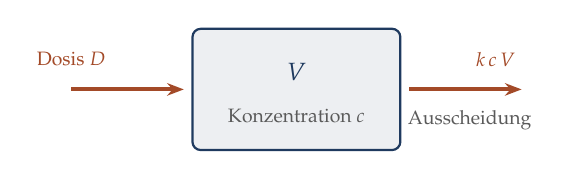
\begin{tikzpicture}[scale=1.1]
\draw[tief, thick, rounded corners=3pt, fill=tief!8] (-1.2,-0.7) rectangle (1.2,0.7);
\node[font=\small, color=tief] at (0,0.2) {$V$};
\node[font=\scriptsize, color=grau] at (0,-0.3) {Konzentration $c$};
\draw[kanted, -{Stealth[length=6pt]}] (-2.6,0) -- (-1.3,0);
\node[font=\scriptsize, color=akzent] at (-2.6,0.35) {Dosis $D$};
\draw[kanted, -{Stealth[length=6pt]}] (1.3,0) -- (2.6,0);
\node[font=\scriptsize, color=akzent] at (2.3,0.35) {$k\,c\,V$};
\node[font=\scriptsize, color=grau] at (2.0,-0.35) {Ausscheidung};
\end{tikzpicture}
\end{center}

\schritt{Was daran offensichtlich falsch ist}
Der Körper ist kein Behälter, und die Verteilung braucht Zeit. Der Abschnitt über den Bruchfall geht dem nach.

\begin{center}
\begin{minipage}{0.88\textwidth}
\kursiv{Das Modell trifft trotzdem für viele Wirkstoffe erstaunlich gut zu --- sobald die Verteilungsphase abgeschlossen ist. Es ist die Grundlage praktisch jeder Dosierungsempfehlung.}
\end{minipage}
\end{center}
\end{merksatz}

\section{Die drei Kenngrößen}

\begin{definition}
\boxtitelm{Definition 10.1}
\begin{center}
{\small
\renewcommand{\arraystretch}{1.6}
\begin{tabular}{@{}P{3.4cm}P{5.2cm}@{}}
\toprule
\textbf{Verteilungs\-volumen $V$} & Das Volumen, in dem sich die Dosis verteilen müsste, um die gemessene Konzentration zu ergeben: $V = D/c_0$.\\
\textbf{Eliminations\-konstante $k$} & Anteil, der je Zeiteinheit ausgeschieden wird.\\
\textbf{Clearance $\mathrm{CL}$} & Volumen, das je Zeiteinheit vollständig vom Wirkstoff befreit wird.\\
\bottomrule
\end{tabular}}
\end{center}
\end{definition}

\begin{merksatz}
\boxtitel{Wie sie zusammenhängen}
\schritt{Die Elimination}
Die Menge im Körper ist $M = c\,V$. Die Ausscheidungsrate beträgt
\[ -\frac{\dd M}{\dd t} = \mathrm{CL}\cdot c , \]
denn je Zeiteinheit wird das Volumen $\mathrm{CL}$ geklärt, jedes mit der Konzentration $c$.

\schritt{Die Gleichung}
\[ V\frac{\dd c}{\dd t} = -\mathrm{CL}\cdot c \quad\Longrightarrow\quad \frac{\dd c}{\dd t} = -\frac{\mathrm{CL}}{V}\,c \]

Das ist die Zerfallsgleichung aus Kapitel~1 mit
\[ \boxed{\;k = \frac{\mathrm{CL}}{V}, \qquad \mathrm{CL} = k\,V, \qquad t_{1/2} = \frac{\ln 2}{k} = \frac{\ln 2 \cdot V}{\mathrm{CL}}\;} \]

\begin{center}
\begin{minipage}{0.88\textwidth}
\kursiv{Von den drei Größen sind nur zwei unabhängig. $V$ und $\mathrm{CL}$ sind die \kursiv{grundlegenden} --- sie haben eine unmittelbare körperliche Bedeutung. Die Halbwertszeit ist eine abgeleitete Größe und kann sich ändern, ohne dass sich die Ausscheidungsleistung ändert: Bei Wassereinlagerung steigt $V$, und $t_{1/2}$ steigt mit, obwohl die Niere unverändert arbeitet.}
\end{minipage}
\end{center}

\schritt{Für den Leitfall}
\[ k = \frac{\ln 2}{4} = 0{,}1733\ \mathrm{h}^{-1} \]
\[ \mathrm{CL} = k\,V = 0{,}1733 \cdot 20 = 3{,}47\ \mathrm{l/h} \]
\[ c_0 = \frac{D}{V} = \frac{640}{20} = 32\ \mathrm{mg/l} \]
--- derselbe Wert wie in Aufgabe 1.2. \checkmark
\end{merksatz}

\section{Die Dauerinfusion}

\begin{merksatz}
\boxtitel{Satz 10.2 --- Anflutung}
Wird der Wirkstoff mit der festen Rate $R$ (Menge je Zeit) infundiert, so gilt
\[ c(t) = \frac{R}{\mathrm{CL}}\left(1 - e^{-kt}\right) . \]

\schritt{Beweis}
Die Gleichung lautet
\[ V\frac{\dd c}{\dd t} = R - \mathrm{CL}\cdot c \quad\Longrightarrow\quad \frac{\dd c}{\dd t} = \frac{R}{V} - k\,c . \]

\kursiv{Trennung der Veränderlichen.} Wir schreiben $c_\infty := R/\mathrm{CL} = R/(kV)$, dann ist
\[ \frac{\dd c}{\dd t} = k\,(c_\infty - c) \]
\[ \frac{\dd c}{c_\infty - c} = k\,\dd t \]

Integrieren --- links mit der Substitution $u = c_\infty - c$, also $\dd u = -\dd c$:
\[ -\ln(c_\infty - c) = kt + C_1 \]
\[ c_\infty - c = A\,e^{-kt} \]

\kursiv{Anfangsbedingung} $c(0) = 0$ liefert $A = c_\infty$:
\[ c(t) = c_\infty\left(1 - e^{-kt}\right) . \qquad \blacksquare \]

\schritt{Die Probe}
\[ \frac{\dd c}{\dd t} = c_\infty\,k\,e^{-kt} \]
\[ k(c_\infty - c) = k\,c_\infty e^{-kt} \quad \checkmark \]
und $c(0) = 0$. \checkmark
\end{merksatz}

\begin{merksatz}
\boxtitel{Der Gleichgewichtsspiegel}
\[ c_\infty = \frac{R}{\mathrm{CL}} \]

\begin{center}
\begin{minipage}{0.9\textwidth}
\textbf{Der Gleichgewichtsspiegel hängt nur von Infusionsrate und Clearance ab --- nicht vom Verteilungsvolumen.}
\end{minipage}
\end{center}

\begin{center}
\begin{minipage}{0.88\textwidth}
\kursiv{Das ist eine der praktisch wichtigsten Aussagen der Pharmakokinetik. Will man einen bestimmten Spiegel halten, so braucht man nur die Clearance zu kennen. Und wenn die Nierenfunktion nachlässt, sinkt $\mathrm{CL}$ --- der Spiegel steigt entsprechend, bei unveränderter Dosis.}
\end{minipage}
\end{center}

\schritt{Für den Leitfall}
Um dauerhaft $20$ mg/l zu halten:
\[ R = \mathrm{CL}\cdot c_\infty = 3{,}47 \cdot 20 = 69{,}3\ \mathrm{mg/h} \]
\end{merksatz}

\begin{merksatz}
\boxtitel{Satz 10.3 --- die Vier-Halbwertszeiten-Regel}
Der Anteil des Endwerts nach $n$ Halbwertszeiten beträgt
\[ 1 - \left(\tfrac12\right)^{n} . \]

\schritt{Beweis}
Nach $n$ Halbwertszeiten ist $t = n\,t_{1/2} = n\ln2/k$, also
\[ e^{-kt} = e^{-n\ln 2} = \left(e^{\ln 2}\right)^{-n} = 2^{-n} = \left(\tfrac12\right)^{n} . \qquad \blacksquare \]

\begin{center}
\renewcommand{\arraystretch}{1.45}
\begin{tabular}{@{}P{2.8cm}P{2.2cm}P{2.4cm}@{}}
\toprule
\textbf{Halbwerts\-zeiten} & \textbf{erreicht} & \\
\midrule
$1$ & $50{,}00\,\%$ & \\
$2$ & $75{,}00\,\%$ & \\
$3$ & $87{,}50\,\%$ & \\
$\mathbf{4}$ & $\mathbf{93{,}75\,\%}$ & \textcolor{gruen}{Faustregel}\\
$5$ & $96{,}88\,\%$ & \\
$7$ & $99{,}22\,\%$ & \\
\bottomrule
\end{tabular}
\end{center}

\begin{center}
\begin{minipage}{0.9\textwidth}
\textbf{Dieselbe Tabelle wie in Kapitel~1, nur von unten gelesen.} Das ist kein Zufall: Die Anflutungskurve ist das Spiegelbild der Abklingkurve.
\end{minipage}
\end{center}

\schritt{Die praktische Folgerung}
\begin{center}
\begin{minipage}{0.88\textwidth}
\kursiv{Nach vier Halbwertszeiten ist das Gleichgewicht praktisch erreicht --- unabhängig von der Dosis. Wer die Infusionsrate verdoppelt, verdoppelt den Endwert, erreicht ihn aber nicht schneller. Für den Leitfall bedeutet das $16$ Stunden; bei Wirkstoffen mit einer Halbwertszeit von Tagen entsprechend Wochen.}
\end{minipage}
\end{center}

\schritt{Die Antwort auf Frage 3 --- die Aufsättigungsdosis}
Will man den Zielspiegel sofort erreichen, gibt man vorweg die Menge, die zu diesem Spiegel gehört:
\[ D_{\text{Auf}} = c_\infty \cdot V = 20 \cdot 20 = 400\ \mathrm{mg} . \]

\begin{center}
\begin{minipage}{0.88\textwidth}
\kursiv{Hier ist es umgekehrt wie beim Gleichgewichtsspiegel: Die Aufsättigungsdosis hängt nur vom \kursiv{Volumen} ab, die Erhaltungsdosis nur von der \kursiv{Clearance}. Zwei verschiedene Fragen, zwei verschiedene Größen --- das ist der Grund, warum man beide getrennt kennt.}
\end{minipage}
\end{center}
\end{merksatz}

\section{Wiederholte Gaben}

\begin{merksatz}
\boxtitel{Satz 10.4 --- der Gleichgewichtszustand}
Wird alle $\tau$ Zeiteinheiten die Dosis $D$ gegeben, so pendeln sich die Spiegel ein bei
\[ c_{\max} = \frac{D/V}{1-r}, \qquad c_{\min} = \frac{(D/V)\,r}{1-r} \qquad\text{mit}\qquad r = e^{-k\tau} . \]

\schritt{Beweis}
Sei $c_n$ der Höchstwert unmittelbar nach der $n$-ten Gabe. Vor der nächsten Gabe ist der Spiegel auf $c_n r$ gefallen, dann kommt $D/V$ hinzu:
\[ c_{n+1} = c_n\,r + \frac{D}{V} \]

Das ist eine Rekursion wie in Kapitel~3. Im Gleichgewicht gilt $c_{n+1} = c_n = c_{\max}$:
\[ c_{\max} = c_{\max}\,r + \frac{D}{V} \quad\Longrightarrow\quad c_{\max}(1-r) = \frac{D}{V} \quad\Longrightarrow\quad c_{\max} = \frac{D/V}{1-r} . \]

Der Tiefstwert ist $c_{\min} = c_{\max}\,r$. $\blacksquare$

\schritt{Die Stabilität}
Nach Satz 3.4 ist der Fixpunkt stabil, wenn $|f'| < 1$. Hier ist $f(c) = cr + D/V$, also $f' = r = e^{-k\tau} < 1$. \checkmark

\schritt{Der Anreicherungsfaktor}
\[ R_{\text{ac}} = \frac{1}{1-r} \]
gibt an, um welchen Faktor der Spitzenspiegel gegenüber der Einzelgabe steigt.
\end{merksatz}

\begin{merksatz}
\boxtitel{Die Antwort auf die Fragen 1 und 2}
Für den Leitfall mit $\tau = 8$ h --- genau zwei Halbwertszeiten:
\[ r = e^{-0{,}1733 \cdot 8} = e^{-1{,}3863} = 0{,}2500 \]

\begin{center}
\begin{minipage}{0.88\textwidth}
\kursiv{Der Wert $0{,}25$ ist exakt, nicht gerundet: Zwei Halbwertszeiten bedeuten Viertelung. Man sollte solche Werte immer über die Halbwertszeiten prüfen --- es ist die schnellste Fehlerkontrolle.}
\end{minipage}
\end{center}

\[ R_{\text{ac}} = \frac{1}{1-0{,}25} = \frac{4}{3} = 1{,}333 \]
\[ c_{\max} = \frac{32}{0{,}75} = 42{,}67\ \mathrm{mg/l}, \qquad c_{\min} = 42{,}67 \cdot 0{,}25 = 10{,}67\ \mathrm{mg/l} \]

\schritt{Der Weg dorthin}
\begin{center}
{\small
\renewcommand{\arraystretch}{1.42}
\begin{tabular}{@{}P{1.4cm}P{1.8cm}P{1.8cm}P{2.4cm}@{}}
\toprule
\textbf{Gabe} & $c_{\max}$ & $c_{\min}$ & \textbf{Anteil am Endwert}\\
\midrule
$1$ & $32{,}00$ & $8{,}00$ & $75{,}0\,\%$\\
$2$ & $40{,}00$ & $10{,}00$ & $93{,}8\,\%$\\
$3$ & $42{,}00$ & $10{,}50$ & $98{,}4\,\%$\\
$4$ & $42{,}50$ & $10{,}62$ & $99{,}6\,\%$\\
$5$ & $42{,}62$ & $10{,}66$ & $99{,}9\,\%$\\
$\infty$ & $\mathbf{42{,}67}$ & $\mathbf{10{,}67}$ & $100\,\%$\\
\bottomrule
\end{tabular}}
\end{center}

\begin{center}
\begin{minipage}{0.9\textwidth}
\textbf{Nach der zweiten Gabe --- also nach $16$ Stunden --- sind $93{,}8\,\%$ erreicht.} Das ist wieder die Vier-Halbwertszeiten-Regel: $16$ h sind vier Halbwertszeiten.
\end{minipage}
\end{center}

\schritt{Die Schwankungsbreite}
\[ \frac{c_{\max}}{c_{\min}} = \frac{1}{r} = e^{k\tau} = 2^{\tau/t_{1/2}} = 2^{2} = 4 \]

\begin{center}
\begin{minipage}{0.88\textwidth}
\kursiv{Die Schwankungsbreite hängt \kursiv{allein} vom Verhältnis aus Dosierungsintervall und Halbwertszeit ab --- nicht von der Dosis. Je Halbwertszeit im Intervall verdoppelt sich das Verhältnis.}
\end{minipage}
\end{center}

\begin{center}
\renewcommand{\arraystretch}{1.45}
\begin{tabular}{@{}P{2.4cm}P{2.2cm}P{2.6cm}@{}}
\toprule
$\tau/t_{1/2}$ & $c_{\max}/c_{\min}$ & \\
\midrule
$0{,}5$ & $1{,}41$ & \textcolor{gruen}{fast gleichmäßig}\\
$1$ & $2$ & \\
$2$ & $4$ & unser Fall\\
$3$ & $8$ & \\
$4$ & $16$ & \textcolor{akzent}{starke Schwankung}\\
\bottomrule
\end{tabular}
\end{center}
\end{merksatz}

\begin{merksatz}
\boxtitel{Die Aufsättigungsdosis bei wiederholter Gabe}
\[ D_{\text{Auf}} = \frac{D}{1-r} = D \cdot R_{\text{ac}} = 640 \cdot 1{,}333 = 853\ \mathrm{mg} \]

Gibt man zuerst $853$ mg und danach alle acht Stunden $640$ mg, so liegt der Spiegel von Anfang an im Gleichgewichtsbereich.

\begin{center}
\begin{minipage}{0.88\textwidth}
\kursiv{Bei einem Anreicherungsfaktor von $1{,}33$ lohnt das kaum. Bei Wirkstoffen mit langer Halbwertszeit und kurzem Intervall wird der Faktor groß --- und dann ist die Aufsättigung unumgänglich, weil man sonst tagelang unwirksam behandelt.}
\end{minipage}
\end{center}

\schritt{Ein Beispiel dazu}
$t_{1/2} = 40$ h, $\tau = 12$ h:
\[ r = 2^{-12/40} = 2^{-0{,}3} = 0{,}812, \qquad R_{\text{ac}} = \frac{1}{0{,}188} = 5{,}32 \]
Ohne Aufsättigung dauerte es $4 \cdot 40 = 160$ Stunden --- fast sieben Tage --- bis zum Gleichgewicht.
\end{merksatz}

\section{Die Gabe durch den Mund}

\begin{merksatz}
\boxtitel{Zwei gegenläufige Vorgänge}
Bei oraler Gabe kommt der Wirkstoff nicht auf einmal an. Man beschreibt die Aufnahme als eigenen Vorgang erster Ordnung mit der Rate $k_a$.

\begin{center}
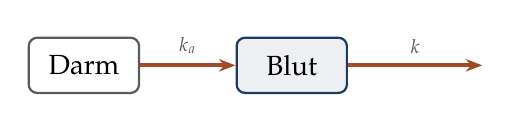
\begin{tikzpicture}[scale=1.1]
\node[draw=grau, thick, rounded corners=3pt, minimum width=1.4cm, minimum height=0.7cm] (G) at (-2.4,0) {Darm};
\node[draw=tief, thick, rounded corners=3pt, minimum width=1.4cm, minimum height=0.7cm, fill=tief!8] (B) at (0,0) {Blut};
\draw[kanted, -{Stealth[length=6pt]}] (G) -- (B) node[midway, above, font=\scriptsize, color=grau] {$k_a$};
\draw[kanted, -{Stealth[length=6pt]}] (B) -- (2.2,0) node[midway, above, font=\scriptsize, color=grau] {$k$};
\end{tikzpicture}
\end{center}

\schritt{Das Ergebnis}
\[ c(t) = \frac{F\,D}{V}\cdot\frac{k_a}{k_a-k}\left(e^{-kt} - e^{-k_a t}\right) \]
mit der \Begriff{Bioverfügbarkeit} $F$ --- dem Anteil, der überhaupt ins Blut gelangt.

Man nennt das die \Begriff{Bateman-Funktion}.

\begin{center}
\begin{minipage}{0.88\textwidth}
\kursiv{Die Herleitung führt auf eine lineare Differentialgleichung mit einem abklingenden Zufluss; sie steht in Band 14, Teil~II. Wir prüfen die Lösung stattdessen an ihren Eigenschaften.}
\end{minipage}
\end{center}

\schritt{Die Probe an $t=0$}
\[ c(0) = \frac{FD}{V}\cdot\frac{k_a}{k_a-k}\,(1-1) = 0 \quad \checkmark \]
Richtig: Unmittelbar nach dem Schlucken ist noch nichts im Blut.

\schritt{Die Probe für große $t$}
Da $k_a > k$, klingt $e^{-k_at}$ schneller ab. Für große $t$ bleibt
\[ c(t) \approx \frac{FD}{V}\cdot\frac{k_a}{k_a-k}\,e^{-kt} , \]
also derselbe Abfall wie bei der Spritze --- nur von einem anderen Ausgangswert. \checkmark
\end{merksatz}

\begin{merksatz}
\boxtitel{Der Gipfel}
\[ t_{\max} = \frac{\ln(k_a/k)}{k_a - k} \]

\schritt{Herleitung}
Ableiten und null setzen:
\[ \frac{\dd c}{\dd t} = \frac{FD}{V}\cdot\frac{k_a}{k_a-k}\left(-k\,e^{-kt} + k_a\,e^{-k_at}\right) \stackrel{!}{=} 0 \]
\[ k_a\,e^{-k_at} = k\,e^{-kt} \quad\Longrightarrow\quad \frac{k_a}{k} = e^{(k_a-k)t} \]
\[ t_{\max} = \frac{\ln(k_a/k)}{k_a-k} . \qquad \blacksquare \]

\schritt{Für den Leitfall}
Mit $k_a = 1{,}0\ \mathrm{h}^{-1}$ und $F = 0{,}8$:
\[ t_{\max} = \frac{\ln(1{,}0/0{,}1733)}{1{,}0-0{,}1733} = \frac{\ln 5{,}770}{0{,}8267} = \frac{1{,}7527}{0{,}8267} = 2{,}12\ \mathrm{h} \]
\[ c_{\max} = 17{,}7\ \mathrm{mg/l} \]

\begin{center}
{\small
\renewcommand{\arraystretch}{1.4}
\begin{tabular}{@{}P{1.4cm}P{1.8cm}P{1.4cm}P{1.8cm}@{}}
\toprule
$t$ (h) & $c$ (mg/l) & $t$ (h) & $c$ (mg/l)\\
\midrule
$0$ & $0{,}00$ & $3$ & $16{,}87$\\
$0{,}5$ & $9{,}61$ & $4$ & $14{,}92$\\
$1$ & $14{,}65$ & $6$ & $10{,}87$\\
$\mathbf{2{,}12}$ & $\mathbf{17{,}73}$ & $8$ & $7{,}73$\\
\bottomrule
\end{tabular}}
\end{center}

\begin{center}
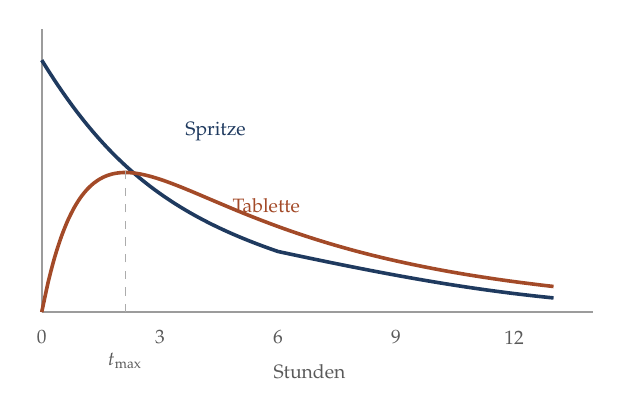
\begin{tikzpicture}[scale=1.0]
\draw[grau!60, line width=0.7pt] (0,0) -- (7.0,0);
\draw[grau!60, line width=0.7pt] (0,0) -- (0,3.6);
\foreach \x/\lab in {0/0, 1.5/3, 3.0/6, 4.5/9, 6.0/12}
  \node[font=\scriptsize, color=grau] at (\x,-0.32) {\lab};
\node[font=\scriptsize, color=grau] at (3.4,-0.75) {Stunden};
\draw[tief, line width=1.3pt] (0,3.2) .. controls (0.8,1.9) and (1.6,1.25) .. (3.0,0.77)
  .. controls (4.4,0.47) and (5.4,0.29) .. (6.5,0.18);
\draw[akzent, line width=1.3pt, smooth, samples=80, domain=0:6.5]
  plot (\x, {2.56*1.2096*(exp(-0.1733*\x*2)-exp(-1.0*\x*2))});
\node[font=\scriptsize, color=tief, anchor=west] at (1.7,2.3) {Spritze};
\node[font=\scriptsize, color=akzent, anchor=west] at (2.3,1.35) {Tablette};
\draw[grau!50, dashed] (1.06,0) -- (1.06,1.85);
\node[font=\scriptsize, color=grau] at (1.06,-0.62) {$t_{\max}$};
\end{tikzpicture}
\end{center}
\end{merksatz}

\begin{merksatz}
\boxtitel{Die Fläche unter der Kurve}
\[ \mathrm{AUC} = \int_0^\infty c(t)\,\dd t = \frac{F\,D}{\mathrm{CL}} \]

\schritt{Warum}
Die insgesamt ausgeschiedene Menge muss der aufgenommenen entsprechen:
\[ F\,D = \int_0^\infty \mathrm{CL}\cdot c(t)\,\dd t = \mathrm{CL}\cdot\mathrm{AUC} . \]

\begin{center}
\begin{minipage}{0.9\textwidth}
\textbf{Die Fläche hängt nur von der aufgenommenen Menge und der Clearance ab --- nicht von der Aufnahmegeschwindigkeit.}
\end{minipage}
\end{center}

\schritt{Für den Leitfall}
\begin{center}
\renewcommand{\arraystretch}{1.48}
\begin{tabular}{@{}P{2.4cm}P{2.6cm}P{2.4cm}@{}}
\toprule
& \textbf{AUC} & $c_{\max}$\\
\midrule
Spritze & $184{,}7$ & $32{,}0$\\
Tablette & $147{,}7$ & $17{,}7$\\
Verhältnis & $0{,}80 = F$ & $0{,}55$\\
\bottomrule
\end{tabular}
\end{center}

\begin{center}
\begin{minipage}{0.88\textwidth}
\kursiv{Das Verhältnis der Flächen ist genau die Bioverfügbarkeit --- und genau so wird sie gemessen. Beim Spitzenspiegel gilt das nicht: Er hängt zusätzlich von der Aufnahmegeschwindigkeit ab. Bei Prüfungen der Austauschbarkeit von Arzneimitteln werden deshalb \kursiv{beide} Größen verglichen.}
\end{minipage}
\end{center}
\end{merksatz}

\section{Der Bruchfall}

\begin{warnung}
\boxtitelr{Vier Stellen, an denen das Modell bricht}
\begin{center}
{\small
\renewcommand{\arraystretch}{1.5}
\begin{tabular}{@{}P{2.4cm}P{3.0cm}P{2.8cm}@{}}
\toprule
\textbf{Verletzung} & \textbf{Wann} & \textbf{Folge}\\
\midrule
Zwei Kammern & Verteilung braucht Zeit & früher Abfall steiler\\
Sättigung & Enzyme ausgelastet & \textcolor{akzent}{Elimination nicht mehr erster Ordnung}\\
Veränderliche Clearance & Nierenfunktion & Spiegel steigt\\
Erster Durchgang & Leberpassage & $F$ klein und schwankend\\
\bottomrule
\end{tabular}}
\end{center}

\schritt{Zur Sättigungskinetik}
Wird der Wirkstoff durch ein Enzym abgebaut, so gilt genauer
\[ -\frac{\dd c}{\dd t} = \frac{V_{\max}\,c}{K_M + c} \]
--- die Michaelis-Menten-Beziehung aus Kapitel~11.

\begin{center}
\renewcommand{\arraystretch}{1.5}
\begin{tabular}{@{}P{2.4cm}P{6.2cm}@{}}
\toprule
$c \ll K_M$ & Nenner $\approx K_M$, also Abbau proportional zu $c$ --- erster Ordnung, wie bisher.\\
$c \gg K_M$ & Nenner $\approx c$, also Abbau $\approx V_{\max}$ --- \kursiv{konstant}, unabhängig von $c$.\\
\bottomrule
\end{tabular}
\end{center}

\begin{center}
\begin{minipage}{0.9\textwidth}
\textbf{Im Sättigungsbereich gibt es keine Halbwertszeit.} Der Spiegel fällt linear statt exponentiell, und eine Dosiserhöhung kann den Spiegel überproportional steigen lassen.
\end{minipage}
\end{center}

\begin{center}
\begin{minipage}{0.88\textwidth}
\kursiv{Das betrifft unter anderem Phenytoin, Alkohol und hochdosierte Salicylate. Bei Alkohol ist es alltäglich bekannt: Der Abbau beträgt etwa $0{,}15$ Promille je Stunde, gleichgültig wie hoch der Spiegel ist. Widmark beschrieb das 1932 --- und nannte damit als Erster einen Wirkstoff, der der Zerfallsgleichung aus Kapitel~1 \kursiv{nicht} folgt.}
\end{minipage}
\end{center}
\end{warnung}

\begin{warnung}
\boxtitelr{Das Zweikammermodell}
Nach einer Spritze fällt der Spiegel zunächst steil, dann flacher. Die erste Phase ist die Verteilung ins Gewebe, die zweite die eigentliche Ausscheidung.

\begin{center}
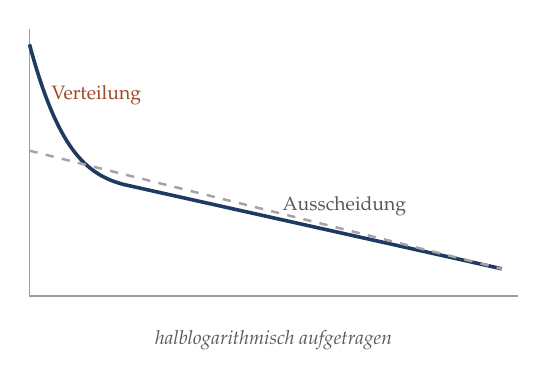
\begin{tikzpicture}[scale=1.0]
\draw[grau!60, line width=0.7pt] (0,0) -- (6.2,0);
\draw[grau!60, line width=0.7pt] (0,0) -- (0,3.4);
\draw[tief, line width=1.3pt]
  (0,3.2) .. controls (0.35,1.9) and (0.7,1.55) .. (1.2,1.42)
  -- (6.0,0.35);
\draw[grau!55, dashed, line width=0.9pt] (0,1.85) -- (6.0,0.35);
\node[font=\scriptsize, color=akzent] at (0.85,2.55) {Verteilung};
\node[font=\scriptsize, color=grau] at (4.0,1.15) {Ausscheidung};
\node[font=\scriptsize\itshape, color=grau] at (3.1,-0.55) {halblogarithmisch aufgetragen};
\end{tikzpicture}
\end{center}

\begin{center}
\begin{minipage}{0.88\textwidth}
\kursiv{In der halblogarithmischen Darstellung aus Kapitel~1 sieht man das sofort: Zwei Geraden statt einer. Die Steigung der zweiten liefert die eigentliche Eliminationskonstante; misst man zu früh, so erhält man eine zu kurze Halbwertszeit und dosiert zu hoch.}
\end{minipage}
\end{center}

\schritt{Die praktische Regel}
Blutspiegel zur Therapiesteuerung werden unmittelbar vor der nächsten Gabe abgenommen --- als Talspiegel. Dann ist die Verteilungsphase sicher vorbei.
\end{warnung}

\section{Übungsaufgaben}

\begin{aufgabe}
\boxtitel{Aufgabe 10.1 --- Dosierung bei eingeschränkter Nierenfunktion}
Ein Wirkstoff wird vollständig über die Niere ausgeschieden. Bei normaler Funktion gilt $\mathrm{CL} = 6{,}0$ l/h und $V = 40$ l. Bei einem Patienten ist die Nierenfunktion auf $40\,\%$ vermindert. Wie ändern sich Halbwertszeit, Erhaltungs- und Aufsättigungsdosis?

\loesung
\schritt{Schritt 1 --- Normalfall}
\[ k = \frac{\mathrm{CL}}{V} = \frac{6{,}0}{40} = 0{,}15\ \mathrm{h}^{-1} \]
\[ t_{1/2} = \frac{\ln 2}{0{,}15} = 4{,}62\ \mathrm{h} \]

\schritt{Schritt 2 --- Eingeschränkte Funktion}
\[ \mathrm{CL} = 0{,}4 \cdot 6{,}0 = 2{,}4\ \mathrm{l/h} \]
Das Verteilungsvolumen ändert sich nicht:
\[ k = \frac{2{,}4}{40} = 0{,}06\ \mathrm{h}^{-1}, \qquad t_{1/2} = \frac{0{,}6931}{0{,}06} = 11{,}55\ \mathrm{h} \]

\schritt{Schritt 3 --- Die Zusammenstellung}
\begin{center}
\renewcommand{\arraystretch}{1.48}
\begin{tabular}{@{}P{2.6cm}P{2.0cm}P{2.0cm}P{1.6cm}@{}}
\toprule
& \textbf{normal} & \textbf{vermindert} & \textbf{Faktor}\\
\midrule
$\mathrm{CL}$ & $6{,}0$ & $2{,}4$ & $0{,}40$\\
$V$ & $40$ & $40$ & $1{,}00$\\
$k$ & $0{,}150$ & $0{,}060$ & $0{,}40$\\
$t_{1/2}$ & $4{,}62$ h & $11{,}55$ h & $\mathbf{2{,}50}$\\
\bottomrule
\end{tabular}
\end{center}

\schritt{Schritt 4 --- Die Erhaltungsdosis}
Der Gleichgewichtsspiegel ist $c_\infty = R/\mathrm{CL}$. Um denselben Spiegel zu halten:
\[ R_{\text{neu}} = 0{,}4 \cdot R_{\text{alt}} \]

\begin{center}
\begin{minipage}{0.9\textwidth}
\textbf{Die Erhaltungsdosis muss auf $40\,\%$ gesenkt werden --- genau im Verhältnis der Clearance.}
\end{minipage}
\end{center}

\schritt{Schritt 5 --- Die Aufsättigungsdosis}
\[ D_{\text{Auf}} = c_{\text{Ziel}}\cdot V \]
$V$ ist unverändert, also bleibt die Aufsättigungsdosis \textbf{gleich}.

\begin{center}
\begin{minipage}{0.88\textwidth}
\kursiv{Das ist die praktisch wichtigste Aussage der Aufgabe und wird regelmäßig falsch gemacht: \textbf{Bei Niereninsuffizienz wird die Erhaltungsdosis angepasst, die Aufsättigungsdosis nicht.} Wer auch die erste Gabe reduziert, erreicht den wirksamen Bereich unter Umständen tagelang nicht --- und bei einer schweren Infektion kann das entscheidend sein.}
\end{minipage}
\end{center}

\schritt{Schritt 6 --- Zwei Wege zur Anpassung}
\begin{center}
\renewcommand{\arraystretch}{1.48}
\begin{tabular}{@{}P{2.6cm}P{2.6cm}P{2.6cm}@{}}
\toprule
\textbf{Verfahren} & \textbf{Dosis} & \textbf{Intervall}\\
\midrule
Dosis senken & $\times 0{,}4$ & unverändert\\
Intervall dehnen & unverändert & $\times 2{,}5$\\
\bottomrule
\end{tabular}
\end{center}

Beide halten den mittleren Spiegel gleich. Sie unterscheiden sich in der Schwankungsbreite:

\begin{center}
\begin{minipage}{0.88\textwidth}
\kursiv{Dosissenkung bei gleichem Intervall ergibt geringere Schwankungen --- richtig bei Wirkstoffen, die dauerhaft über einer Schwelle liegen müssen. Intervalldehnung ergibt hohe Spitzen und tiefe Täler --- richtig bei Wirkstoffen, deren Wirkung von der Spitzenkonzentration abhängt und deren Giftigkeit vom Talspiegel. Bei Aminoglykosiden trifft genau das zu, und deshalb dehnt man dort das Intervall.}
\end{minipage}
\end{center}
\end{aufgabe}

\begin{aufgabe}
\boxtitel{Aufgabe 10.2 --- Ein Dosierungsschema entwerfen}
Ein Antibiotikum soll dauerhaft zwischen $5$ und $20$ mg/l liegen. Bekannt: $t_{1/2} = 6$ h, $V = 35$ l. Bestimmen Sie Intervall und Dosis.

\loesung
\schritt{Schritt 1 --- Die Schwankungsbreite festlegen}
\[ \frac{c_{\max}}{c_{\min}} = \frac{20}{5} = 4 \]

\schritt{Schritt 2 --- Das Intervall}
Nach Abschnitt 10.4 ist
\[ \frac{c_{\max}}{c_{\min}} = 2^{\tau/t_{1/2}} \quad\Longrightarrow\quad 4 = 2^{\tau/6} \quad\Longrightarrow\quad \frac{\tau}{6} = 2 \quad\Longrightarrow\quad \tau = 12\ \mathrm{h} \]

\textbf{Zweimal täglich.}

\schritt{Schritt 3 --- Die Dosis}
\[ r = e^{-k\tau} = 2^{-2} = 0{,}25 \]
\[ c_{\max} = \frac{D/V}{1-r} \quad\Longrightarrow\quad 20 = \frac{D/35}{0{,}75} \]
\[ \frac{D}{35} = 20 \cdot 0{,}75 = 15 \quad\Longrightarrow\quad D = 525\ \mathrm{mg} \]

\schritt{Schritt 4 --- Die Proben}
\[ c_{\max} = \frac{525/35}{0{,}75} = \frac{15}{0{,}75} = 20{,}0 \quad \checkmark \]
\[ c_{\min} = 20{,}0 \cdot 0{,}25 = 5{,}0 \quad \checkmark \]

\schritt{Schritt 5 --- Die Aufsättigung}
\[ D_{\text{Auf}} = \frac{525}{0{,}75} = 700\ \mathrm{mg} \]

\kursiv{Probe:} $700/35 = 20$ mg/l unmittelbar nach der Gabe --- genau der Zielhöchstwert. \checkmark

\schritt{Schritt 6 --- Der Verlauf ohne Aufsättigung}
\begin{center}
\renewcommand{\arraystretch}{1.42}
\begin{tabular}{@{}P{1.4cm}P{1.8cm}P{1.8cm}P{2.2cm}@{}}
\toprule
\textbf{Gabe} & $c_{\max}$ & $c_{\min}$ & \textbf{im Zielbereich?}\\
\midrule
$1$ & $15{,}0$ & $3{,}75$ & \textcolor{akzent}{nein}\\
$2$ & $18{,}75$ & $4{,}69$ & \textcolor{akzent}{knapp nicht}\\
$3$ & $19{,}69$ & $4{,}92$ & \textcolor{mittel}{fast}\\
$4$ & $19{,}92$ & $4{,}98$ & \textcolor{gruen}{ja}\\
\bottomrule
\end{tabular}
\end{center}

\begin{center}
\begin{minipage}{0.88\textwidth}
\kursiv{Ohne Aufsättigung liegt der Talspiegel in den ersten zwei Tagen unter der Wirkschwelle. Bei einer schweren Infektion sind das zwei verlorene Tage --- genau dann, wenn die Erregerlast am größten ist.}
\end{minipage}
\end{center}

\schritt{Schritt 7 --- Eine Alternative prüfen}
Wäre $\tau = 8$ h besser?
\[ r = 2^{-8/6} = 2^{-1{,}333} = 0{,}397, \qquad \frac{c_{\max}}{c_{\min}} = 2{,}52 \]
Mit $c_{\min} = 5$: $c_{\max} = 12{,}6$ --- deutlich unter $20$.
\[ D = c_{\max}\,V\,(1-r) = 12{,}6 \cdot 35 \cdot 0{,}603 = 266\ \mathrm{mg} \]

\begin{center}
\renewcommand{\arraystretch}{1.48}
\begin{tabular}{@{}P{2.0cm}P{2.0cm}P{2.2cm}P{2.2cm}@{}}
\toprule
$\tau$ & \textbf{Dosis} & \textbf{Tagesdosis} & \textbf{Spanne}\\
\midrule
$12$ h & $525$ mg & $1050$ mg & $5$--$20$\\
$8$ h & $266$ mg & $798$ mg & $5$--$12{,}6$\\
\bottomrule
\end{tabular}
\end{center}

\begin{center}
\begin{minipage}{0.86\textwidth}
\kursiv{Das kürzere Intervall braucht ein Viertel weniger Wirkstoff für denselben Talspiegel --- weil weniger im hohen Bereich verschwendet wird. Dafür muss dreimal täglich gegeben werden, was die Zuverlässigkeit der Einnahme mindert. Diese Abwägung ist keine Rechenfrage.}
\end{minipage}
\end{center}
\end{aufgabe}

\begin{aufgabe}
\boxtitel{Aufgabe 10.3 --- Wann die Halbwertszeit täuscht}
Bei einem Patienten wird eine verlängerte Halbwertszeit gemessen. Zeigen Sie an zwei Fällen, dass daraus \kursiv{nicht} auf eine verminderte Ausscheidung zu schließen ist.

\loesung
\schritt{Schritt 1 --- Die Grundbeziehung}
\[ t_{1/2} = \frac{\ln 2 \cdot V}{\mathrm{CL}} \]

Die Halbwertszeit steigt, wenn $V$ steigt \kursiv{oder} $\mathrm{CL}$ fällt.

\schritt{Schritt 2 --- Fall A: verminderte Clearance}
Ausgangswerte $V = 30$ l, $\mathrm{CL} = 5$ l/h:
\[ t_{1/2} = \frac{0{,}693 \cdot 30}{5} = 4{,}16\ \mathrm{h} \]
Bei halbierter Clearance:
\[ t_{1/2} = \frac{0{,}693 \cdot 30}{2{,}5} = 8{,}32\ \mathrm{h} \]

\schritt{Schritt 3 --- Fall B: vergrößertes Verteilungsvolumen}
Etwa bei ausgeprägter Wassereinlagerung: $V = 60$ l bei unveränderter Clearance:
\[ t_{1/2} = \frac{0{,}693 \cdot 60}{5} = 8{,}32\ \mathrm{h} \]

\textbf{Dieselbe Halbwertszeit, völlig verschiedene Ursache.}

\schritt{Schritt 4 --- Die Folgen für die Dosierung}
\begin{center}
{\small
\renewcommand{\arraystretch}{1.5}
\begin{tabular}{@{}P{2.4cm}P{1.6cm}P{2.0cm}P{2.1cm}@{}}
\toprule
& \textbf{Ausgang} & \textbf{Fall A} & \textbf{Fall B}\\
\midrule
$V$ & $30$ & $30$ & $\mathbf{60}$\\
$\mathrm{CL}$ & $5$ & $\mathbf{2{,}5}$ & $5$\\
$t_{1/2}$ & $4{,}16$ & $8{,}32$ & $8{,}32$\\
\midrule
Erhaltungs\-dosis & --- & \textcolor{akzent}{halbieren} & \textcolor{gruen}{unverändert}\\
Aufsättigungs\-dosis & --- & \textcolor{gruen}{unverändert} & \textcolor{akzent}{verdoppeln}\\
\bottomrule
\end{tabular}}
\end{center}

\schritt{Schritt 5 --- Die Deutung}
\begin{center}
\begin{minipage}{0.9\textwidth}
\textbf{Die Anpassungen sind genau entgegengesetzt.} Wer beide Fälle verwechselt, dosiert in beide Richtungen falsch.
\end{minipage}
\end{center}

\begin{center}
\begin{minipage}{0.88\textwidth}
\kursiv{Daraus folgt die Regel, die am Anfang von Abschnitt 10.2 stand: Man denkt in $V$ und $\mathrm{CL}$, nicht in der Halbwertszeit. Die Halbwertszeit ist eine abgeleitete Größe und sagt für sich genommen nichts darüber, was zu tun ist.}
\end{minipage}
\end{center}

\schritt{Schritt 6 --- Wie man die Fälle unterscheidet}
Man misst den Spiegel unmittelbar nach einer bekannten Dosis:
\[ V = \frac{D}{c_0} \]

Ist $c_0$ niedriger als erwartet, liegt Fall B vor. Ist $c_0$ normal und der Abfall verlangsamt, liegt Fall A vor.

\begin{center}
\begin{minipage}{0.86\textwidth}
\kursiv{Bei Schwerkranken auf der Intensivstation treten beide Veränderungen häufig gemeinsam auf --- vergrößertes Verteilungsvolumen durch Flüssigkeitstherapie und veränderte Clearance. Deshalb wird dort bei mehreren Antibiotika der Spiegel gemessen statt nach Tabelle dosiert.}
\end{minipage}
\end{center}
\end{aufgabe}

\begin{geschichte}
\boxtitelg{Von der Blutalkoholbestimmung zur Arzneimitteldosierung}
\Person{Erik Widmark} (1889--1945), schwedischer Rechtsmediziner, untersuchte in den 1920er Jahren den Abbau von Alkohol. Er fand, dass der Blutspiegel \kursiv{linear} fällt --- nicht exponentiell --- und stellte 1932 die nach ihm benannte Formel auf.

\begin{center}
\begin{minipage}{0.9\textwidth}
\kursiv{Widmark führte dabei den Begriff des Verteilungsvolumens ein, wenn auch unter anderem Namen: Sein Faktor $\varrho$ ist das Verteilungsvolumen je Kilogramm Körpergewicht. Er ist bei Frauen kleiner als bei Männern, weil Alkohol sich nicht im Fettgewebe verteilt --- die erste Anwendung eines pharmakokinetischen Parameters auf Unterschiede zwischen Personengruppen.}
\end{minipage}
\end{center}

\schritt{Die Begründung des Fachs}
\Person{Friedrich Hartmut Dost} (1910--1985), Kinderarzt in Leipzig und später Gießen, prägte 1953 den Begriff \kursiv{Pharmakokinetik} und schrieb das erste Lehrbuch dazu.

\begin{center}
\begin{minipage}{0.9\textwidth}
\kursiv{Sein Ausgangspunkt war ein klinisches Bedürfnis: Kinder sind keine kleinen Erwachsenen, und die Umrechnung der Dosis nach Körpergewicht führte regelmäßig zu falschen Spiegeln. Dost zeigte, dass man Volumen und Clearance getrennt betrachten muss --- genau die Unterscheidung aus Aufgabe 10.3.}
\end{minipage}
\end{center}

\schritt{Die Funktion}
\Person{Harry Bateman} (1882--1946), britischer Mathematiker, leitete die nach ihm benannte Funktion 1910 her --- für radioaktive Zerfallsreihen, in denen ein Stoff entsteht und zugleich zerfällt.

\begin{center}
\begin{minipage}{0.9\textwidth}
\kursiv{Dass dieselbe Gleichung die Aufnahme einer Tablette beschreibt, bemerkte man erst Jahrzehnte später. Es ist wieder das Muster aus Kapitel~6: Die Mathematik ist lange vor der Anwendung da.}
\end{minipage}
\end{center}
\end{geschichte}

\begin{forschung}
\boxtitelp{Pharmakokinetik heute}
\begin{center}
{\small
\renewcommand{\arraystretch}{1.45}
\begin{tabular}{@{}P{2.8cm}P{5.4cm}@{}}
\toprule
\textbf{Bevölkerungs\-modelle} & Statt eines Patienten modelliert man eine ganze Gruppe und schätzt, wie stark die Parameter zwischen Personen streuen --- die Mehrebenenmodelle aus Band 17, Kapitel~11.\\
\textbf{Physiologisch begründete Modelle} & Ein Kompartiment je Organ, mit gemessenen Durchblutungen. Erlaubt Vorhersagen ohne Versuche am Menschen.\\
\textbf{Spiegelsteuerung} & Messung und Anpassung während der Behandlung, zunehmend rechnergestützt.\\
\bottomrule
\end{tabular}}
\end{center}

\schritt{Zur ersten Zeile}
Der entscheidende Fortschritt: Man kann aus wenigen Messungen je Patient, aber vielen Patienten, die Verteilung der Parameter schätzen --- und daraus für einen neuen Patienten eine Vorhersage ableiten, die mit jeder Messung genauer wird.

\begin{center}
\begin{minipage}{0.88\textwidth}
\kursiv{Das ist der bayessche Zugang aus Band 17, Kapitel~5: Die Bevölkerungsverteilung ist die Vorwissensverteilung, die Messung am einzelnen Patienten die Beobachtung. Eine einzige Spiegelmessung liefert dann eine erheblich bessere Dosisempfehlung als jede Tabelle.}
\end{minipage}
\end{center}

\schritt{Was bei Antibiotika besonders zählt}
Bei Antibiotika reicht der Spiegel allein nicht --- entscheidend ist sein Verhältnis zur Empfindlichkeit des Erregers.

\begin{center}
{\small
\renewcommand{\arraystretch}{1.45}
\begin{tabular}{@{}P{3.0cm}P{5.2cm}@{}}
\toprule
\textbf{Zeitabhängig} & Wirkung hängt davon ab, wie lange der Spiegel über der Hemmkonzentration liegt --- kurze Intervalle oder Dauerinfusion.\\
\textbf{Spiegel\-abhängig} & Wirkung hängt von der Spitze ab --- lange Intervalle, hohe Einzeldosen.\\
\bottomrule
\end{tabular}}
\end{center}

\begin{center}
\begin{minipage}{0.88\textwidth}
\kursiv{Diese Unterscheidung erklärt die Empfehlung aus Aufgabe 10.1, bei Aminoglykosiden das Intervall zu dehnen statt die Dosis zu senken --- und sie ist der Grund, warum bei Betalaktamen zunehmend über Dauerinfusion nachgedacht wird. Kapitel~14 verbindet das mit der Resistenzentwicklung.}
\end{minipage}
\end{center}
\end{forschung}

\begin{merksatz}
\boxtitel{Was Sie jetzt können}
\begin{center}
\renewcommand{\arraystretch}{1.5}
\begin{tabular}{@{}P{3.2cm}P{5.4cm}@{}}
\toprule
\textbf{Definition 10.1} & $\mathrm{CL} = kV$; nur zwei sind unabhängig\\
\textbf{Satz 10.2} & Anflutung $c_\infty(1-e^{-kt})$\\
\textbf{Satz 10.3} & vier Halbwertszeiten bis zum Gleichgewicht\\
\textbf{Satz 10.4} & $c_{\max} = (D/V)/(1-r)$; Schwankung $2^{\tau/t_{1/2}}$\\
\textbf{Getrennt denken} & Erhaltungsdosis aus $\mathrm{CL}$, Aufsättigung aus $V$\\
\bottomrule
\end{tabular}
\end{center}

\begin{center}
\begin{minipage}{0.88\textwidth}
\kursiv{Im nächsten Kapitel gehen wir eine Ebene tiefer: zu den Enzymen und Rezeptoren, an denen der Wirkstoff angreift --- und zu der Sättigungskurve, die in diesem Kapitel schon aufgetaucht ist.}
\end{minipage}
\end{center}
\end{merksatz}

\chapter{Enzym- und Rezeptorkinetik}

\section{Warum Sättigung}

\begin{merksatz}
\boxtitel{Der Leitfall, eine Ebene tiefer}
Kapitel~10 behandelte den Wirkstoff als Menge in einem Behälter. Jetzt fragen wir, was ihn abbaut --- und woran er wirkt.

\begin{center}
\begin{minipage}{0.9\textwidth}
Beides sind \kursiv{Bindungsvorgänge}: Ein Enzym bindet den Wirkstoff und baut ihn ab; ein Rezeptor bindet ihn und löst eine Wirkung aus. Die Mathematik ist in beiden Fällen dieselbe.
\end{minipage}
\end{center}

\schritt{Die entscheidende Einsicht}
\begin{center}
\begin{minipage}{0.9\textwidth}
\textbf{Es gibt nur endlich viele Enzym- und Rezeptormoleküle. Sind sie alle besetzt, kann mehr Substrat nichts mehr bewirken.}
\end{minipage}
\end{center}

Daraus folgt eine Sättigungskurve --- und damit der Grund, warum das Modell aus Kapitel~1 bei hohen Konzentrationen bricht.
\end{merksatz}

\begin{merksatz}
\boxtitel{Das Reaktionsschema}
\begin{center}
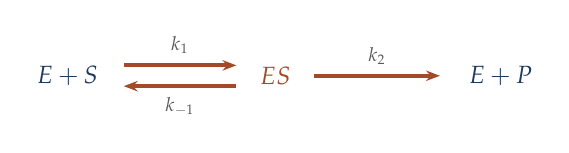
\begin{tikzpicture}[scale=1.1]
\node[font=\small, color=tief] (ES1) at (-2.4,0) {$E + S$};
\node[font=\small, color=akzent] (ES) at (0,0) {$ES$};
\node[font=\small, color=tief] (EP) at (2.6,0) {$E + P$};
\draw[kanted, -{Stealth[length=5pt]}] (-1.75,0.12) -- (-0.45,0.12) node[midway, above, font=\scriptsize, color=grau] {$k_1$};
\draw[kanted, -{Stealth[length=5pt]}] (-0.45,-0.12) -- (-1.75,-0.12) node[midway, below, font=\scriptsize, color=grau] {$k_{-1}$};
\draw[kanted, -{Stealth[length=5pt]}] (0.45,0) -- (1.9,0) node[midway, above, font=\scriptsize, color=grau] {$k_2$};
\end{tikzpicture}
\end{center}

\begin{center}
{\small
\renewcommand{\arraystretch}{1.48}
\begin{tabular}{@{}P{1.4cm}P{3.0cm}P{3.6cm}@{}}
\toprule
$E$ & freies Enzym & bindet\\
$S$ & Substrat & wird umgesetzt\\
$ES$ & Komplex & Zwischenzustand\\
$P$ & Erzeugnis & verlässt das Enzym\\
\bottomrule
\end{tabular}}
\end{center}

\schritt{Die Erhaltungsgröße}
Die Gesamtmenge an Enzym bleibt fest:
\[ [E] + [ES] = E_0 . \]

\begin{center}
\begin{minipage}{0.88\textwidth}
\kursiv{Das ist dieselbe Art von Probe wie bei den Kammermodellen in Kapitel~7: Was nicht frei ist, ist gebunden. Wer sie nicht aufstellt, verliert die entscheidende Beziehung.}
\end{minipage}
\end{center}
\end{merksatz}

\section{Die Michaelis-Menten-Gleichung}

\begin{merksatz}
\boxtitel{Satz 11.1}
Unter der Annahme, dass sich die Komplexmenge rasch einstellt und danach nahezu unverändert bleibt, gilt für die Umsatzgeschwindigkeit
\[ v \;=\; \frac{V_{\max}\,[S]}{K_M + [S]} \]
mit
\[ V_{\max} = k_2\,E_0 \qquad\text{und}\qquad K_M = \frac{k_{-1}+k_2}{k_1} . \]
\end{merksatz}

\begin{merksatz}
\boxtitel{Beweis}
\schritt{Schritt 1 --- Die Gleichung für den Komplex}
Der Komplex entsteht durch Bindung und zerfällt auf zwei Wegen:
\[ \frac{\dd[ES]}{\dd t} = \underbrace{k_1[E][S]}_{\text{Bildung}} - \underbrace{k_{-1}[ES]}_{\text{Zerfall zurück}} - \underbrace{k_2[ES]}_{\text{Umsatz}} \]

\schritt{Schritt 2 --- Die Annahme}
Nach kurzer Anlaufzeit ändert sich $[ES]$ kaum noch:
\[ \frac{\dd[ES]}{\dd t} \approx 0 \]

Man nennt das die \Begriff{Quasi-Stationarität}.

\begin{center}
\begin{minipage}{0.88\textwidth}
\kursiv{Sie ist gerechtfertigt, wenn das Substrat weit im Überschuss vorliegt --- dann ändert es sich langsam, und der Komplex folgt ihm nahezu augenblicklich. Das ist derselbe Gedanke wie bei der Trennung schneller und langsamer Vorgänge in der Pharmakokinetik.}
\end{minipage}
\end{center}

\schritt{Schritt 3 --- Auflösen}
\[ k_1[E][S] = (k_{-1}+k_2)[ES] \]

Mit $[E] = E_0 - [ES]$:
\[ k_1\bigl(E_0 - [ES]\bigr)[S] = (k_{-1}+k_2)[ES] \]
\[ k_1E_0[S] = (k_{-1}+k_2)[ES] + k_1[ES][S] \]
\[ k_1E_0[S] = [ES]\bigl(k_{-1}+k_2+k_1[S]\bigr) \]

Durch $k_1$ teilen:
\[ E_0[S] = [ES]\left(\frac{k_{-1}+k_2}{k_1} + [S]\right) = [ES]\bigl(K_M + [S]\bigr) \]
\[ [ES] = \frac{E_0\,[S]}{K_M+[S]} \]

\schritt{Schritt 4 --- Die Geschwindigkeit}
Das Erzeugnis entsteht mit der Rate
\[ v = k_2[ES] = \frac{k_2E_0\,[S]}{K_M+[S]} = \frac{V_{\max}[S]}{K_M+[S]} . \qquad \blacksquare \]
\end{merksatz}

\begin{merksatz}
\boxtitel{Was die beiden Parameter bedeuten}
\schritt{$V_{\max}$ --- die Höchstgeschwindigkeit}
Für $[S] \to \infty$ geht $\frac{[S]}{K_M+[S]} \to 1$, also $v \to V_{\max}$.

Sie hängt von der Enzymmenge ab: $V_{\max} = k_2E_0$. Doppelt so viel Enzym, doppelte Höchstgeschwindigkeit.

\schritt{$K_M$ --- die Halbsättigungskonzentration}
Setzt man $[S] = K_M$:
\[ v = \frac{V_{\max}K_M}{K_M+K_M} = \frac{V_{\max}}{2} \]

\begin{center}
\begin{minipage}{0.9\textwidth}
\textbf{$K_M$ ist diejenige Substratkonzentration, bei der die halbe Höchstgeschwindigkeit erreicht wird.}
\end{minipage}
\end{center}

\begin{center}
{\small
\renewcommand{\arraystretch}{1.45}
\begin{tabular}{@{}P{2.4cm}P{2.2cm}P{2.8cm}@{}}
\toprule
$[S]$ & $v/V_{\max}$ & \\
\midrule
$0{,}1\,K_M$ & $9{,}1\,\%$ & \\
$0{,}5\,K_M$ & $33{,}3\,\%$ & \\
$K_M$ & $\mathbf{50{,}0\,\%}$ & \\
$2\,K_M$ & $66{,}7\,\%$ & \\
$4\,K_M$ & $80{,}0\,\%$ & \\
$10\,K_M$ & $90{,}9\,\%$ & \\
$40\,K_M$ & $97{,}6\,\%$ & \\
\bottomrule
\end{tabular}}
\end{center}

\begin{center}
\begin{minipage}{0.88\textwidth}
\kursiv{Die Kurve nähert sich der Höchstgeschwindigkeit sehr langsam. Um von $90$ auf $98$ Prozent zu kommen, braucht man die vierfache Substratkonzentration. Deshalb lässt sich $V_{\max}$ aus Messwerten nur schlecht ablesen --- man erreicht es nie.}
\end{minipage}
\end{center}

\begin{center}
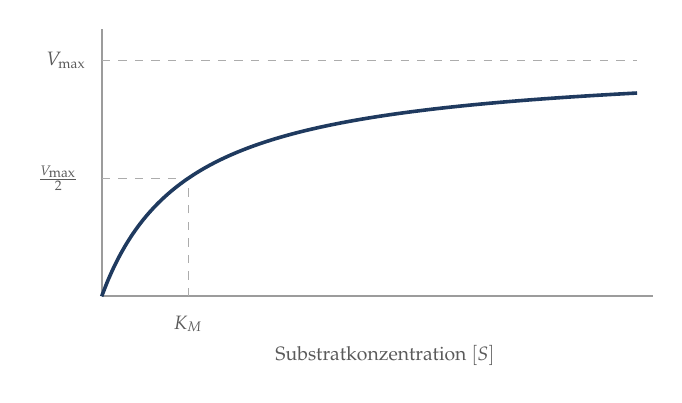
\begin{tikzpicture}[scale=1.0]
\draw[grau!60, line width=0.7pt] (0,0) -- (7.0,0);
\draw[grau!60, line width=0.7pt] (0,0) -- (0,3.4);
\draw[grau!50, dashed] (0,3.0) -- (6.8,3.0);
\node[font=\scriptsize, color=grau] at (-0.45,3.0) {$V_{\max}$};
\draw[grau!50, dashed] (0,1.5) -- (1.1,1.5);
\draw[grau!50, dashed] (1.1,0) -- (1.1,1.5);
\node[font=\scriptsize, color=grau] at (-0.55,1.5) {$\frac{V_{\max}}{2}$};
\node[font=\scriptsize, color=grau] at (1.1,-0.35) {$K_M$};
\draw[tief, line width=1.3pt, smooth, samples=90, domain=0:6.8]
  plot (\x, {3.0*\x/(1.1+\x)});
\node[font=\scriptsize, color=grau] at (3.6,-0.75) {Substratkonzentration $[S]$};
\end{tikzpicture}
\end{center}
\end{merksatz}

\begin{merksatz}
\boxtitel{Die zwei Bereiche}
\begin{center}
{\small
\renewcommand{\arraystretch}{1.5}
\begin{tabular}{@{}P{2.4cm}P{2.8cm}P{3.0cm}@{}}
\toprule
\textbf{Bereich} & \textbf{Näherung} & \textbf{Verhalten}\\
\midrule
$[S] \ll K_M$ & $v \approx \frac{V_{\max}}{K_M}[S]$ & \textcolor{gruen}{erster Ordnung}\\
$[S] \gg K_M$ & $v \approx V_{\max}$ & \textcolor{akzent}{nullter Ordnung}\\
\bottomrule
\end{tabular}}
\end{center}

\begin{center}
\begin{minipage}{0.9\textwidth}
\textbf{Im unteren Bereich ist die Gleichung aus Kapitel~1 richtig, im oberen nicht.} Das ist die Auflösung des Bruchfalls aus Kapitel~10.
\end{minipage}
\end{center}

\schritt{Die Folge für den Wirkstoffabbau}
\begin{center}
\renewcommand{\arraystretch}{1.5}
\begin{tabular}{@{}P{2.6cm}P{6.0cm}@{}}
\toprule
\textbf{Niedriger Spiegel} & Halbwertszeit ist eine sinnvolle Größe; alles aus Kapitel~10 gilt.\\
\textbf{Hoher Spiegel} & Der Abbau ist \kursiv{konstant}. Es gibt keine Halbwertszeit; der Spiegel fällt linear.\\
\bottomrule
\end{tabular}
\end{center}

\begin{center}
\begin{minipage}{0.88\textwidth}
\kursiv{Beim Alkohol liegt der übliche Bereich weit über $K_M$ --- daher der gleichmäßige Abbau von etwa $0{,}15$ Promille je Stunde. Bei Phenytoin liegt der therapeutische Bereich \kursiv{genau im Übergang}, und das macht diesen Wirkstoff so schwierig: Eine kleine Dosiserhöhung kann den Spiegel überproportional steigen lassen.}
\end{minipage}
\end{center}
\end{merksatz}

\section{Hemmung}

\begin{merksatz}
\boxtitel{Zwei Arten, ein Enzym zu bremsen}
\begin{center}
{\small
\renewcommand{\arraystretch}{1.55}
\begin{tabular}{@{}P{2.4cm}P{2.8cm}P{3.0cm}@{}}
\toprule
& \textbf{Kompetitiv} & \textbf{Nichtkompetitiv}\\
\midrule
Bindungsort & derselbe wie Substrat & anderer Ort\\
$V_{\max}$ & \textcolor{gruen}{unverändert} & \textcolor{akzent}{sinkt}\\
$K_M$ & \textcolor{akzent}{steigt} & \textcolor{gruen}{unverändert}\\
Überwindbar & \textcolor{gruen}{ja, durch mehr Substrat} & \textcolor{akzent}{nein}\\
\bottomrule
\end{tabular}}
\end{center}

\schritt{Kompetitive Hemmung}
\[ v = \frac{V_{\max}[S]}{K_M\left(1+\frac{[I]}{K_i}\right) + [S]} \]

Der Hemmstoff wirkt so, als wäre $K_M$ um den Faktor $1+[I]/K_i$ größer.

\schritt{Nichtkompetitive Hemmung}
\[ v = \frac{\frac{V_{\max}}{1+[I]/K_i}\,[S]}{K_M + [S]} \]

Hier sinkt $V_{\max}$, als hätte man Enzym entfernt.
\end{merksatz}

\begin{merksatz}
\boxtitel{Der Unterschied in Zahlen}
$V_{\max}=100$, $K_M=25$, $K_i=10$.

\begin{center}
{\small
\renewcommand{\arraystretch}{1.48}
\begin{tabular}{@{}P{1.6cm}P{2.0cm}P{2.0cm}P{2.2cm}@{}}
\toprule
$[I]$ & $K_{M,\text{eff}}$ & $v$ bei $[S]=25$ & $v$ bei $[S]=1000$\\
\midrule
$0$ & $25$ & $50{,}0$ & $97{,}6$\\
$10$ & $50$ & $33{,}3$ & $95{,}2$\\
$30$ & $100$ & $20{,}0$ & $90{,}9$\\
$90$ & $250$ & $9{,}1$ & $80{,}0$\\
\bottomrule
\end{tabular}}
\end{center}

\begin{center}
\begin{minipage}{0.9\textwidth}
\textbf{Bei niedriger Substratkonzentration hemmt der Stoff auf ein Fünftel; bei hoher kaum noch.} Genau das meint \enquote{überwindbar}.
\end{minipage}
\end{center}

\begin{center}
\begin{minipage}{0.88\textwidth}
\kursiv{Das ist klinisch folgenreich: Bei einer Vergiftung mit einem kompetitiven Hemmstoff kann man das natürliche Substrat im Überschuss zuführen und den Hemmstoff verdrängen. Bei Methanolvergiftung gibt man Ethanol, das um dasselbe Enzym konkurriert --- und verhindert so die Bildung des giftigen Abbauprodukts. Bei nichtkompetitiver Hemmung wirkt dieses Vorgehen nicht.}
\end{minipage}
\end{center}
\end{merksatz}

\begin{warnung}
\boxtitelr{Die Linearisierung nach Lineweaver und Burk}
Bildet man Kehrwerte, so wird aus der Sättigungskurve eine Gerade:
\[ \frac{1}{v} = \frac{K_M}{V_{\max}}\cdot\frac{1}{[S]} + \frac{1}{V_{\max}} \]

\schritt{Die Herleitung}
\[ \frac{1}{v} = \frac{K_M+[S]}{V_{\max}[S]} = \frac{K_M}{V_{\max}[S]} + \frac{[S]}{V_{\max}[S]} \]

Trägt man $1/v$ gegen $1/[S]$ auf, so ist der Achsenabschnitt $1/V_{\max}$ und die Steigung $K_M/V_{\max}$.

\schritt{Warum man das heute nicht mehr tut}
\begin{center}
\renewcommand{\arraystretch}{1.5}
\begin{tabular}{@{}P{3.0cm}P{5.6cm}@{}}
\toprule
\textbf{Fehler\-verzerrung} & Kleine Messwerte von $v$ werden zu großen Werten von $1/v$ --- gerade die unsichersten Punkte bestimmen die Gerade.\\
\textbf{Ungleiche Streuung} & Die Voraussetzung gleicher Streuung aus Band 17, Kapitel~10 ist verletzt.\\
\textbf{Hebelwirkung} & Der Punkt bei kleinstem $[S]$ liegt am weitesten rechts und hat die größte Hebelwirkung.\\
\bottomrule
\end{tabular}
\end{center}

\begin{center}
\begin{minipage}{0.88\textwidth}
\kursiv{Man passt die Sättigungskurve heute unmittelbar an, mit nichtlinearer Regression. Die Darstellung nach Lineweaver und Burk ist trotzdem nützlich --- nicht zum Schätzen, sondern zum \kursiv{Erkennen}: Kompetitive und nichtkompetitive Hemmung erzeugen dort unterscheidbare Geradenbüschel.}
\end{minipage}
\end{center}

\begin{center}
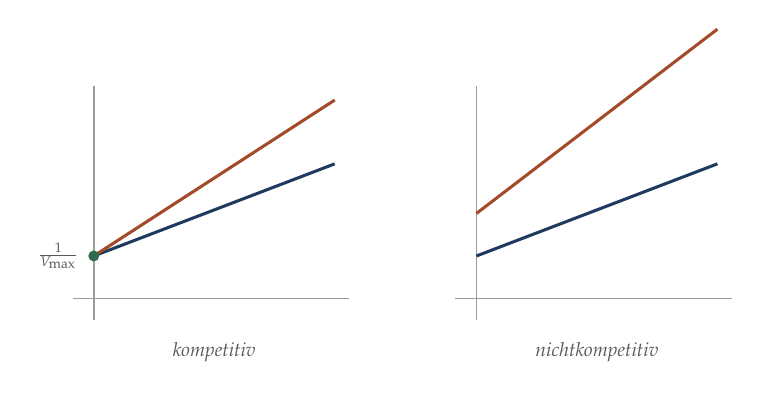
\begin{tikzpicture}[scale=0.9]
\begin{scope}
\draw[grau!60, line width=0.6pt] (-0.3,0) -- (3.6,0);
\draw[grau!60, line width=0.6pt] (0,-0.3) -- (0,3.0);
\draw[tief, line width=1.1pt] (0,0.6) -- (3.4,1.9);
\draw[akzent, line width=1.1pt] (0,0.6) -- (3.4,2.8);
\fill[gruen] (0,0.6) circle (2.2pt);
\node[font=\scriptsize\itshape, color=grau] at (1.7,-0.75) {kompetitiv};
\node[font=\scriptsize, color=grau] at (-0.5,0.6) {$\frac{1}{V_{\max}}$};
\end{scope}
\begin{scope}[xshift=5.4cm]
\draw[grau!60, line width=0.6pt] (-0.3,0) -- (3.6,0);
\draw[grau!60, line width=0.6pt] (0,-0.3) -- (0,3.0);
\draw[tief, line width=1.1pt] (0,0.6) -- (3.4,1.9);
\draw[akzent, line width=1.1pt] (0,1.2) -- (3.4,3.8);
\node[font=\scriptsize\itshape, color=grau] at (1.7,-0.75) {nichtkompetitiv};
\end{scope}
\end{tikzpicture}
\end{center}

Links schneiden sich alle Geraden auf der senkrechten Achse --- $V_{\max}$ bleibt gleich. Rechts nicht.
\end{warnung}

\section{Kooperativität und die Hill-Gleichung}

\begin{merksatz}
\boxtitel{Wenn Bindungsstellen sich beeinflussen}
Manche Moleküle haben mehrere Bindungsstellen, die einander begünstigen: Ist eine besetzt, binden die übrigen leichter.

\begin{center}
\begin{minipage}{0.9\textwidth}
Der Sättigungsanteil folgt dann der \Begriff{Hill-Gleichung}
\[ \theta = \frac{[L]^{n}}{K^{n} + [L]^{n}} \]
mit dem \Begriff{Hill-Koeffizienten} $n$.
\end{minipage}
\end{center}

\begin{center}
{\small
\renewcommand{\arraystretch}{1.48}
\begin{tabular}{@{}P{1.6cm}P{2.8cm}P{3.2cm}@{}}
\toprule
$n$ & \textbf{Bedeutung} & \textbf{Kurvenform}\\
\midrule
$1$ & keine Kooperativität & Michaelis-Menten\\
$>1$ & positiv kooperativ & \textcolor{akzent}{$S$-förmig}\\
$<1$ & negativ kooperativ & flacher\\
\bottomrule
\end{tabular}}
\end{center}

\begin{center}
\begin{minipage}{0.88\textwidth}
\kursiv{$n$ ist \kursiv{keine} Zahl von Bindungsstellen, sondern ein Maß für die Stärke der Wechselwirkung. Hämoglobin hat vier Bindungsstellen und einen Hill-Koeffizienten von etwa $2{,}8$ --- die Kooperativität ist stark, aber nicht vollständig.}
\end{minipage}
\end{center}
\end{merksatz}

\begin{merksatz}
\boxtitel{Wozu Kooperativität gut ist --- am Hämoglobin}
$K = P_{50} = 26$ mmHg, $n = 2{,}8$. Zum Vergleich dieselbe Halbsättigung mit $n=1$.

\begin{center}
{\small
\renewcommand{\arraystretch}{1.48}
\begin{tabular}{@{}P{2.4cm}P{2.0cm}P{2.2cm}P{2.0cm}@{}}
\toprule
\textbf{Ort} & $p\mathrm{O}_2$ & $n = 2{,}8$ & $n = 1$\\
\midrule
Lunge & $100$ & $\mathbf{97{,}8\,\%}$ & $79{,}4\,\%$\\
Gewebe, Ruhe & $40$ & $77{,}0\,\%$ & $60{,}6\,\%$\\
Muskel, Arbeit & $20$ & $\mathbf{32{,}4\,\%}$ & $43{,}5\,\%$\\
\bottomrule
\end{tabular}}
\end{center}

\schritt{Was abgegeben wird}
\begin{center}
\renewcommand{\arraystretch}{1.48}
\begin{tabular}{@{}P{2.8cm}P{2.2cm}P{2.2cm}@{}}
\toprule
& $n = 2{,}8$ & $n = 1$\\
\midrule
Lunge $\to$ Ruhe & $20{,}8\,\%$ & $18{,}8\,\%$\\
Lunge $\to$ Arbeit & $\mathbf{65{,}3\,\%}$ & $35{,}9\,\%$\\
\bottomrule
\end{tabular}
\end{center}

\begin{center}
\begin{minipage}{0.9\textwidth}
\textbf{Bei starker Beanspruchung gibt die kooperative Bindung fast doppelt so viel Sauerstoff ab.}
\end{minipage}
\end{center}

\schritt{Warum}
Die $S$-Form bewirkt zweierlei zugleich:

\begin{center}
\renewcommand{\arraystretch}{1.5}
\begin{tabular}{@{}P{2.4cm}P{6.2cm}@{}}
\toprule
\textbf{Oben flach} & Bei hohem Angebot fast vollständige Beladung --- und unempfindlich gegen Schwankungen.\\
\textbf{Mitte steil} & Im Gewebebereich führt ein kleiner Druckabfall zu großer Abgabe.\\
\bottomrule
\end{tabular}
\end{center}

\begin{center}
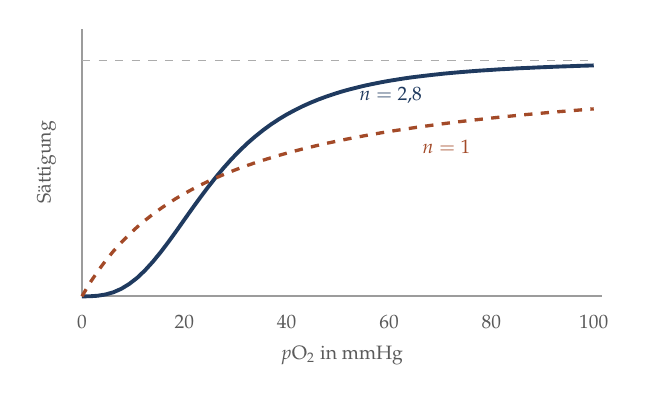
\begin{tikzpicture}[scale=1.0]
\draw[grau!60, line width=0.7pt] (0,0) -- (6.6,0);
\draw[grau!60, line width=0.7pt] (0,0) -- (0,3.4);
\foreach \x/\lab in {0/0, 1.3/20, 2.6/40, 3.9/60, 5.2/80, 6.5/100}
  \node[font=\scriptsize, color=grau] at (\x,-0.32) {\lab};
\draw[grau!50, dashed] (0,3.0) -- (6.5,3.0);
\draw[tief, line width=1.4pt] (0.000,0.000) -- (0.100,0.001) -- (0.200,0.008) -- (0.300,0.024) -- (0.400,0.052) -- (0.500,0.096) -- (0.600,0.157) -- (0.700,0.234) -- (0.800,0.329) -- (0.900,0.439) -- (1.000,0.561) -- (1.100,0.693) -- (1.200,0.831) -- (1.300,0.973) -- (1.400,1.114) -- (1.500,1.252) -- (1.600,1.385) -- (1.700,1.512) -- (1.800,1.632) -- (1.900,1.744) -- (2.000,1.847) -- (2.100,1.943) -- (2.200,2.030) -- (2.300,2.110) -- (2.400,2.183) -- (2.500,2.249) -- (2.600,2.309) -- (2.700,2.363) -- (2.800,2.413) -- (2.900,2.458) -- (3.000,2.499) -- (3.100,2.536) -- (3.200,2.570) -- (3.300,2.601) -- (3.400,2.629) -- (3.500,2.654) -- (3.600,2.678) -- (3.700,2.699) -- (3.800,2.719) -- (3.900,2.737) -- (4.000,2.753) -- (4.100,2.769) -- (4.200,2.783) -- (4.300,2.795) -- (4.400,2.807) -- (4.500,2.818) -- (4.600,2.829) -- (4.700,2.838) -- (4.800,2.847) -- (4.900,2.855) -- (5.000,2.863) -- (5.100,2.870) -- (5.200,2.876) -- (5.300,2.883) -- (5.400,2.888) -- (5.500,2.894) -- (5.600,2.899) -- (5.700,2.903) -- (5.800,2.908) -- (5.900,2.912) -- (6.000,2.916) -- (6.100,2.920) -- (6.200,2.923) -- (6.300,2.927) -- (6.400,2.930) -- (6.500,2.933);
\draw[akzent, line width=1.2pt, dashed] (0.000,0.000) -- (0.100,0.168) -- (0.200,0.317) -- (0.300,0.452) -- (0.400,0.574) -- (0.500,0.685) -- (0.600,0.786) -- (0.700,0.879) -- (0.800,0.964) -- (0.900,1.042) -- (1.000,1.115) -- (1.100,1.183) -- (1.200,1.246) -- (1.300,1.304) -- (1.400,1.359) -- (1.500,1.411) -- (1.600,1.459) -- (1.700,1.504) -- (1.800,1.547) -- (1.900,1.588) -- (2.000,1.626) -- (2.100,1.662) -- (2.200,1.697) -- (2.300,1.729) -- (2.400,1.760) -- (2.500,1.790) -- (2.600,1.818) -- (2.700,1.845) -- (2.800,1.871) -- (2.900,1.895) -- (3.000,1.919) -- (3.100,1.942) -- (3.200,1.963) -- (3.300,1.984) -- (3.400,2.004) -- (3.500,2.023) -- (3.600,2.042) -- (3.700,2.059) -- (3.800,2.077) -- (3.900,2.093) -- (4.000,2.109) -- (4.100,2.124) -- (4.200,2.139) -- (4.300,2.154) -- (4.400,2.167) -- (4.500,2.181) -- (4.600,2.194) -- (4.700,2.207) -- (4.800,2.219) -- (4.900,2.231) -- (5.000,2.242) -- (5.100,2.253) -- (5.200,2.264) -- (5.300,2.275) -- (5.400,2.285) -- (5.500,2.295) -- (5.600,2.305) -- (5.700,2.314) -- (5.800,2.323) -- (5.900,2.332) -- (6.000,2.341) -- (6.100,2.349) -- (6.200,2.357) -- (6.300,2.365) -- (6.400,2.373) -- (6.500,2.381);
\node[font=\scriptsize, color=tief, anchor=west] at (3.4,2.55) {$n=2{,}8$};
\node[font=\scriptsize, color=akzent, anchor=west] at (4.2,1.9) {$n=1$};
\node[font=\scriptsize, color=grau] at (3.3,-0.75) {$p\mathrm{O}_2$ in mmHg};
\node[font=\scriptsize, color=grau, rotate=90] at (-0.45,1.7) {Sättigung};
\end{tikzpicture}
\end{center}

\begin{center}
\begin{minipage}{0.88\textwidth}
\kursiv{Ein Molekül ohne Kooperativität kann nur eines von beidem: entweder fest binden und schlecht abgeben, oder locker binden und schlecht beladen. Die $S$-Form löst diesen Widerspruch --- und sie ist deshalb in der Biologie überall dort zu finden, wo ein Schalter gebraucht wird.}
\end{minipage}
\end{center}
\end{merksatz}

\begin{merksatz}
\boxtitel{Wo die Hill-Gleichung sonst auftaucht}
\begin{center}
{\small
\renewcommand{\arraystretch}{1.48}
\begin{tabular}{@{}P{2.6cm}P{5.6cm}@{}}
\toprule
\textbf{Dosis-Wirkung} & Die Wirkung eines Arzneimittels folgt derselben Form; $K$ heißt dort $\mathrm{EC}_{50}$.\\
\textbf{Genregulation} & Mehrere Regulatormoleküle binden gemeinsam --- die Steilheit erzeugt Schaltverhalten.\\
\textbf{Ionenkanäle} & Öffnungswahrscheinlichkeit in Abhängigkeit von Spannung oder Botenstoff.\\
\bottomrule
\end{tabular}}
\end{center}

\begin{center}
\begin{minipage}{0.88\textwidth}
\kursiv{Die erste Zeile ist der Grund, warum Dosis-Wirkungs-Kurven üblicherweise gegen den \kursiv{Logarithmus} der Dosis aufgetragen werden: In dieser Darstellung wird die Hill-Kurve punktsymmetrisch und im mittleren Bereich annähernd gerade --- was das Ablesen der $\mathrm{EC}_{50}$ erleichtert. Es ist dieselbe Überlegung wie bei der logistischen Kurve in Kapitel~2, deren Symmetrie in Aufgabe 2.3 bewiesen wurde.}
\end{minipage}
\end{center}
\end{merksatz}

\section{Der Bruchfall}

\begin{warnung}
\boxtitelr{Wann die Quasi-Stationarität nicht gilt}
Die Herleitung setzt voraus, dass $[ES]$ sich rasch einstellt und danach kaum ändert. Das verlangt
\[ E_0 \ll [S] + K_M . \]

\begin{center}
\begin{minipage}{0.9\textwidth}
\textbf{Das Enzym muss selten sein gegenüber dem Substrat.} In der Zelle trifft das oft \kursiv{nicht} zu: Manche Enzyme liegen in ähnlicher Menge vor wie ihre Substrate.
\end{minipage}
\end{center}

\begin{center}
\begin{minipage}{0.88\textwidth}
\kursiv{Dann bindet das Enzym einen erheblichen Teil des Substrats, und die frei messbare Konzentration ist kleiner als die Gesamtmenge. Für solche Fälle gibt es erweiterte Formeln; die Michaelis-Menten-Gleichung liefert dort systematisch zu kleine Umsatzraten.}
\end{minipage}
\end{center}
\end{warnung}

\begin{warnung}
\boxtitelr{Und drei weitere Einschränkungen}
\begin{center}
{\small
\renewcommand{\arraystretch}{1.5}
\begin{tabular}{@{}P{2.4cm}P{3.0cm}P{2.8cm}@{}}
\toprule
\textbf{Annahme} & \textbf{Verletzung} & \textbf{Folge}\\
\midrule
Kein Rückweg & $P$ kann zurückreagieren & gilt nur zu Beginn\\
Ein Substrat & meist zwei oder mehr & eigene Formeln nötig\\
Gut durchmischt & Zelle ist es nicht & örtliche Unterschiede\\
\bottomrule
\end{tabular}}
\end{center}

\schritt{Zur ersten Zeile}
Alle Messungen zur Bestimmung von $K_M$ und $V_{\max}$ werden als \Begriff{Anfangsgeschwindigkeit} durchgeführt --- in den ersten Augenblicken, bevor sich nennenswert Erzeugnis angesammelt hat.

\begin{center}
\begin{minipage}{0.88\textwidth}
\kursiv{Das ist keine Feinheit, sondern die Voraussetzung dafür, dass die gemessene Größe überhaupt das ist, was die Gleichung beschreibt. Wer zu spät misst, erhält zu kleine Werte --- und die Abweichung wächst mit der Zeit.}
\end{minipage}
\end{center}

\schritt{Zur dritten Zeile}
In der Zelle sind Enzyme oft in Komplexen zusammengefasst, und die Erzeugnisse werden unmittelbar weitergereicht.

\begin{center}
\begin{minipage}{0.88\textwidth}
\kursiv{Dann gilt das Massenwirkungsgesetz aus Kapitel~4 nicht mehr --- dieselbe Einschränkung, die dort das Räuber-Beute-Modell betraf. Es ist bemerkenswert, wie oft die Durchmischungsannahme in diesem Band die schwächste Stelle ist: bei Populationen, bei Epidemien, im Behälter und nun in der Zelle.}
\end{minipage}
\end{center}
\end{warnung}

\section{Übungsaufgaben}

\begin{aufgabe}
\boxtitel{Aufgabe 11.1 --- Parameter aus Messwerten}
Für ein Enzym wurden gemessen:
\begin{center}
{\small
\renewcommand{\arraystretch}{1.4}
\begin{tabular}{@{}P{2.2cm}P{1.4cm}P{1.4cm}P{1.4cm}P{1.4cm}@{}}
\toprule
$[S]$ (µmol/l) & $10$ & $25$ & $50$ & $200$\\
$v$ (µmol/min) & $28{,}6$ & $50{,}0$ & $66{,}7$ & $88{,}9$\\
\bottomrule
\end{tabular}}
\end{center}
Bestimmen Sie $K_M$ und $V_{\max}$.

\loesung
\schritt{Schritt 1 --- Zwei Gleichungen aufstellen}
Aus zwei Messpunkten lassen sich beide Parameter bestimmen. Wir nehmen $[S]=10$ und $[S]=200$:
\[ 28{,}6 = \frac{V_{\max}\cdot 10}{K_M+10}, \qquad 88{,}9 = \frac{V_{\max}\cdot 200}{K_M+200} \]

\schritt{Schritt 2 --- Umformen}
\[ 28{,}6\,(K_M+10) = 10\,V_{\max} \quad\Longrightarrow\quad V_{\max} = 2{,}86\,K_M + 28{,}6 \]
\[ 88{,}9\,(K_M+200) = 200\,V_{\max} \quad\Longrightarrow\quad V_{\max} = 0{,}4445\,K_M + 88{,}9 \]

\schritt{Schritt 3 --- Gleichsetzen}
\[ 2{,}86\,K_M + 28{,}6 = 0{,}4445\,K_M + 88{,}9 \]
\[ 2{,}4155\,K_M = 60{,}3 \]
\[ K_M = 24{,}96 \approx 25 \ \text{µmol/l} \]

\schritt{Schritt 4 --- $V_{\max}$}
\[ V_{\max} = 2{,}86 \cdot 25 + 28{,}6 = 71{,}5 + 28{,}6 = 100{,}1 \approx 100 \ \text{µmol/min} \]

\schritt{Schritt 5 --- Die Proben an den übrigen Punkten}
\begin{center}
\renewcommand{\arraystretch}{1.42}
\begin{tabular}{@{}P{1.8cm}P{2.2cm}P{2.2cm}P{1.4cm}@{}}
\toprule
$[S]$ & \textbf{gemessen} & \textbf{berechnet} & \\
\midrule
$10$ & $28{,}6$ & $\frac{100\cdot10}{35} = 28{,}6$ & \checkmark\\
$25$ & $50{,}0$ & $\frac{100\cdot25}{50} = 50{,}0$ & \checkmark\\
$50$ & $66{,}7$ & $\frac{100\cdot50}{75} = 66{,}7$ & \checkmark\\
$200$ & $88{,}9$ & $\frac{100\cdot200}{225} = 88{,}9$ & \checkmark\\
\bottomrule
\end{tabular}
\end{center}

\schritt{Schritt 6 --- Die Kontrolle über $K_M$}
Bei $[S] = 25 = K_M$ muss $v = V_{\max}/2 = 50$ sein. Gemessen: $50{,}0$. \checkmark

\schritt{Schritt 7 --- Eine Warnung zur Methode}
Aus zwei Punkten zwei Parameter zu bestimmen funktioniert nur bei fehlerfreien Werten. Bei echten Messdaten passt man alle Punkte gemeinsam an --- mit nichtlinearer Regression, nicht über Kehrwerte.

\begin{center}
\begin{minipage}{0.86\textwidth}
\kursiv{Und man achtet darauf, dass die Messpunkte den Bereich um $K_M$ abdecken. Liegen alle Werte weit darunter, so sieht man nur den linearen Anfangsbereich, und $V_{\max}$ ist praktisch nicht bestimmbar --- dieselbe Schwierigkeit wie bei der Kapazitätsgrenze in Kapitel~2.}
\end{minipage}
\end{center}
\end{aufgabe}

\begin{aufgabe}
\boxtitel{Aufgabe 11.2 --- Eine Hemmung einordnen}
In Gegenwart eines Hemmstoffs werden gemessen: bei $[S]=25$ ein Wert von $v=25{,}0$, bei $[S]=1000$ ein Wert von $v=97{,}6$. Ohne Hemmstoff galt $V_{\max}=100$, $K_M=25$. Welche Art der Hemmung liegt vor?

\loesung
\schritt{Schritt 1 --- Der hohe Wert entscheidet}
Bei $[S]=1000$ ohne Hemmstoff:
\[ v = \frac{100 \cdot 1000}{25+1000} = 97{,}6 \]
Gemessen mit Hemmstoff: ebenfalls $97{,}6$.

\begin{center}
\begin{minipage}{0.9\textwidth}
\textbf{$V_{\max}$ ist unverändert} --- bei hohem Substratüberschuss ist die Hemmung vollständig überwunden.
\end{minipage}
\end{center}

Das spricht für \textbf{kompetitive Hemmung.}

\schritt{Schritt 2 --- Den Faktor bestimmen}
Bei $[S]=25$:
\[ 25{,}0 = \frac{100 \cdot 25}{K_{M,\text{eff}}+25} \]
\[ K_{M,\text{eff}}+25 = \frac{2500}{25} = 100 \quad\Longrightarrow\quad K_{M,\text{eff}} = 75 \]

\schritt{Schritt 3 --- Der Hemmfaktor}
\[ \frac{K_{M,\text{eff}}}{K_M} = \frac{75}{25} = 3{,}0 = 1 + \frac{[I]}{K_i} \]
\[ \frac{[I]}{K_i} = 2{,}0 \]

Die Hemmstoffkonzentration beträgt also das Doppelte der Hemmkonstante.

\schritt{Schritt 4 --- Die Probe bei $[S]=1000$}
\[ v = \frac{100 \cdot 1000}{75+1000} = \frac{100\,000}{1075} = 93{,}0 \]

Hmm --- gemessen wurde $97{,}6$, berechnet $93{,}0$.

\schritt{Schritt 5 --- Der Widerspruch aufgelöst}
Die Abweichung zeigt, dass die Annahme reiner kompetitiver Hemmung nicht ganz trifft. Prüfen wir die Alternative:

\kursiv{Nichtkompetitiv} mit unverändertem $K_M$: Bei $[S]=25$ wäre
\[ 25{,}0 = \frac{V_{\max,\text{eff}}\cdot25}{50} \quad\Longrightarrow\quad V_{\max,\text{eff}} = 50 \]
Dann wäre bei $[S]=1000$:
\[ v = \frac{50\cdot1000}{1025} = 48{,}8 \]
--- weit unter dem gemessenen Wert.

\begin{center}
\renewcommand{\arraystretch}{1.48}
\begin{tabular}{@{}P{2.8cm}P{2.2cm}P{2.4cm}@{}}
\toprule
\textbf{Annahme} & \textbf{Vorhersage} & \textbf{gemessen $97{,}6$}\\
\midrule
kompetitiv & $93{,}0$ & \textcolor{gruen}{nahe}\\
nichtkompetitiv & $48{,}8$ & \textcolor{akzent}{weit daneben}\\
\bottomrule
\end{tabular}
\end{center}

\textbf{Es ist kompetitive Hemmung}, mit einer kleinen Messabweichung im hohen Bereich.

\schritt{Schritt 6 --- Die Lehre}
\begin{center}
\begin{minipage}{0.88\textwidth}
\kursiv{Die Unterscheidung der Hemmarten gelingt nur, wenn man bei \kursiv{hoher} Substratkonzentration misst. Zwei Messpunkte im mittleren Bereich lassen beide Deutungen zu. Das ist eine allgemeine Regel für die Versuchsplanung: Man misst dort, wo sich die Vorhersagen der konkurrierenden Modelle am stärksten unterscheiden.}
\end{minipage}
\end{center}
\end{aufgabe}

\begin{aufgabe}
\boxtitel{Aufgabe 11.3 --- Die Steilheit einer Hill-Kurve}
Zeigen Sie, dass bei der Hill-Gleichung das Verhältnis der Konzentrationen für $90\,\%$ und $10\,\%$ Sättigung
\[ \frac{[L]_{90}}{[L]_{10}} = 81^{1/n} \]
beträgt, und werten Sie es für $n=1$, $n=2{,}8$ und $n=8$ aus.

\loesung
\schritt{Schritt 1 --- Die Gleichung nach $[L]$ auflösen}
\[ \theta = \frac{[L]^n}{K^n+[L]^n} \]
\[ \theta\,(K^n+[L]^n) = [L]^n \]
\[ \theta\,K^n = [L]^n(1-\theta) \]
\[ [L]^n = K^n\,\frac{\theta}{1-\theta} \]
\[ [L] = K\left(\frac{\theta}{1-\theta}\right)^{1/n} \]

\schritt{Schritt 2 --- Die beiden Werte}
\[ [L]_{90} = K\left(\frac{0{,}9}{0{,}1}\right)^{1/n} = K\cdot 9^{1/n} \]
\[ [L]_{10} = K\left(\frac{0{,}1}{0{,}9}\right)^{1/n} = K\cdot 9^{-1/n} \]

\schritt{Schritt 3 --- Das Verhältnis}
\[ \frac{[L]_{90}}{[L]_{10}} = \frac{9^{1/n}}{9^{-1/n}} = 9^{2/n} = \left(9^2\right)^{1/n} = 81^{1/n} . \qquad \blacksquare \]

\schritt{Schritt 4 --- Die Werte}
\begin{center}
\renewcommand{\arraystretch}{1.48}
\begin{tabular}{@{}P{1.6cm}P{2.4cm}P{3.0cm}@{}}
\toprule
$n$ & $81^{1/n}$ & \\
\midrule
$1$ & $81{,}0$ & \textcolor{akzent}{sehr flach}\\
$2{,}8$ & $4{,}94$ & Hämoglobin\\
$4$ & $3{,}00$ & \\
$8$ & $1{,}73$ & \textcolor{gruen}{fast ein Schalter}\\
$\infty$ & $1{,}00$ & idealer Schalter\\
\bottomrule
\end{tabular}
\end{center}

\kursiv{Rechnung für $n=2{,}8$:} $81^{1/2{,}8} = e^{\ln81/2{,}8} = e^{4{,}394/2{,}8} = e^{1{,}569} = 4{,}80$.

\schritt{Schritt 5 --- Die Deutung}
\begin{center}
\begin{minipage}{0.9\textwidth}
\textbf{Ohne Kooperativität braucht man die $81$-fache Konzentration, um von zehn auf neunzig Prozent zu kommen.} Bei $n=8$ genügt weniger als das Doppelte.
\end{minipage}
\end{center}

\schritt{Schritt 6 --- Was das für Arzneimittel bedeutet}
Eine Dosis-Wirkungs-Kurve mit $n=1$ ist flach: Zwischen kaum wirksam und fast voll wirksam liegen fast zwei Zehnerpotenzen.

\begin{center}
\renewcommand{\arraystretch}{1.48}
\begin{tabular}{@{}P{2.0cm}P{3.0cm}P{2.6cm}@{}}
\toprule
$n$ & \textbf{Dosisspanne} & \textbf{Steuerbarkeit}\\
\midrule
$1$ & Faktor $81$ & \textcolor{gruen}{gut steuerbar}\\
$4$ & Faktor $3$ & \\
$8$ & Faktor $1{,}7$ & \textcolor{akzent}{schwer dosierbar}\\
\bottomrule
\end{tabular}
\end{center}

\begin{center}
\begin{minipage}{0.88\textwidth}
\kursiv{Hier kehrt sich die Bewertung um: Was beim Hämoglobin ein Vorteil ist --- der scharfe Umschlag ---, ist beim Arzneimittel ein Nachteil. Eine steile Dosis-Wirkungs-Kurve bedeutet, dass zwischen unwirksam und überdosiert wenig Raum liegt. Bei Wirkstoffen mit hohem Hill-Koeffizienten ist die Dosisfindung entsprechend heikel.}
\end{minipage}
\end{center}
\end{aufgabe}

\begin{geschichte}
\boxtitelg{Eine Arbeit von 1913 und ihre Autorin}
\Person{Leonor Michaelis} (1875--1949), Arzt und Biochemiker in Berlin, und \Person{Maud Menten} (1879--1960), kanadische Ärztin, veröffentlichten 1913 die Arbeit \kursiv{Die Kinetik der Invertinwirkung} --- auf Deutsch, in der \kursiv{Biochemischen Zeitschrift}.

\begin{center}
\begin{minipage}{0.9\textwidth}
\kursiv{Maud Menten gehörte zu den ersten Frauen in Kanada, die Medizin studieren durften. Da Frauen dort keine Forschung betreiben durften, ging sie nach Berlin. Sie promovierte später in Chicago, arbeitete über vierzig Jahre als Pathologin in Pittsburgh und wurde erst 1949 --- im Alter von siebzig Jahren --- zur ordentlichen Professorin ernannt.}
\end{minipage}
\end{center}

\schritt{Die Korrektur von 1925}
Michaelis und Menten nahmen an, dass sich zwischen $E$, $S$ und $ES$ ein \kursiv{Gleichgewicht} einstellt --- das gilt nur, wenn $k_2 \ll k_{-1}$.

\Person{George Briggs} und \Person{John Haldane} ersetzten das 1925 durch die Quasi-Stationarität, die in Satz 11.1 verwendet wurde. Dadurch wurde aus der Dissoziationskonstante $k_{-1}/k_1$ die heutige Größe
\[ K_M = \frac{k_{-1}+k_2}{k_1} . \]

\begin{center}
\begin{minipage}{0.9\textwidth}
\kursiv{Die Form der Gleichung blieb unverändert --- nur die Deutung von $K_M$ änderte sich. Deshalb ist $K_M$ \kursiv{keine} Bindungsstärke, auch wenn es oft so gelesen wird. Es wird nur dann zur Bindungskonstante, wenn der Umsatz langsam gegenüber dem Rückzerfall ist.}
\end{minipage}
\end{center}

\schritt{Die Hill-Gleichung}
\Person{Archibald Hill} veröffentlichte seine Gleichung 1910 --- als Student, in einer halbseitigen Mitteilung, zur Beschreibung der Sauerstoffbindung des Hämoglobins.

\begin{center}
\begin{minipage}{0.9\textwidth}
\kursiv{Er hielt $n$ zunächst für die Zahl der gleichzeitig bindenden Moleküle und war irritiert, dass sich keine ganze Zahl ergab. Die richtige Deutung --- als Maß für die Wechselwirkung --- kam erst später. Hill erhielt 1922 den Nobelpreis für ganz andere Arbeiten, über die Wärmeentwicklung im Muskel.}
\end{minipage}
\end{center}
\end{geschichte}

\begin{forschung}
\boxtitelp{Enzymkinetik heute}
\begin{center}
{\small
\renewcommand{\arraystretch}{1.45}
\begin{tabular}{@{}P{2.8cm}P{5.4cm}@{}}
\toprule
\textbf{Einzelmolekül\-messungen} & Man beobachtet einzelne Enzymmoleküle und findet, dass ihre Umsatzraten über die Zeit schwanken --- ein Molekül hat ein \enquote{Gedächtnis}.\\
\textbf{Vollständige Zellmodelle} & Alle Stoffwechselwege einer Zelle als Gleichungssystem; Hunderte von Parametern, die meisten geschätzt.\\
\textbf{Enzymentwurf} & Rechnergestützter Entwurf neuer Enzyme mit gewünschtem $K_M$ und $V_{\max}$.\\
\bottomrule
\end{tabular}}
\end{center}

\schritt{Zur ersten Zeile}
Die klassische Kinetik beschreibt den Mittelwert über Milliarden von Molekülen. Einzelmolekülmessungen zeigten ab etwa 1998, dass die Mittelung etwas verdeckt: Ein Enzymmolekül wechselt zwischen Zuständen verschiedener Aktivität und bleibt in jedem für Sekunden bis Minuten.

\begin{center}
\begin{minipage}{0.88\textwidth}
\kursiv{Bemerkenswert ist, dass die gemittelte Kurve trotzdem der Michaelis-Menten-Form folgt. Die Gleichung bleibt richtig; ihre Herleitung war es aus dem falschen Grund. Das ist ein wiederkehrendes Muster in diesem Band: Ein Modell kann zutreffen, obwohl sein Mechanismus anders ist als angenommen.}
\end{minipage}
\end{center}

\schritt{Zur zweiten Zeile}
Modelle des gesamten Zellstoffwechsels umfassen heute Tausende von Reaktionen. Die Schwierigkeit liegt nicht im Aufstellen, sondern im Bestimmen der Parameter.

\begin{center}
\begin{minipage}{0.88\textwidth}
\kursiv{Das ist die dritte Warnung aus dem Vorwort in ihrer schärfsten Form: Ein Modell mit tausend Gleichungen und achthundert geschätzten Parametern lässt sich an fast jede Beobachtung anpassen --- und sagt deshalb wenig vorher. Der Gegenentwurf sind Verfahren, die ohne kinetische Parameter auskommen und nur die Stoffbilanzen nutzen; sie sagen weniger, aber das Gesagte ist belastbar.}
\end{minipage}
\end{center}
\end{forschung}

\begin{merksatz}
\boxtitel{Was Sie jetzt können}
\begin{center}
\renewcommand{\arraystretch}{1.5}
\begin{tabular}{@{}P{3.0cm}P{5.6cm}@{}}
\toprule
\textbf{Satz 11.1} & Michaelis-Menten über Quasi-Stationarität\\
\textbf{$K_M$} & Halbsättigung --- keine Bindungsstärke\\
\textbf{Zwei Bereiche} & erster Ordnung unten, nullter oben\\
\textbf{Hemmung} & kompetitiv überwindbar, nichtkompetitiv nicht\\
\textbf{Hill} & Steilheit $81^{1/n}$; Kooperativität als Schalter\\
\bottomrule
\end{tabular}
\end{center}

\begin{center}
\begin{minipage}{0.88\textwidth}
\kursiv{Im nächsten Kapitel bauen wir aus Ionenkanälen, die genau solchen Kurven folgen, ein System, das von selbst Erregungen erzeugt --- und begegnen dabei der Hopf-Bifurkation aus Kapitel~6 wieder.}
\end{minipage}
\end{center}
\end{merksatz}

\chapter{Erregbare Zellen}

\section{Die Frage}

\begin{merksatz}
\boxtitel{Alles oder nichts}
Eine Nervenzelle antwortet auf einen schwachen Reiz mit einer kleinen, rasch abklingenden Spannungsänderung. Überschreitet der Reiz eine Schwelle, so antwortet sie mit einem \Begriff{Aktionspotential}: einem großen, immer gleich geformten Ausschlag.

\begin{center}
\begin{minipage}{0.9\textwidth}
\textbf{Die Antwort hängt nicht von der Reizstärke ab --- nur davon, ob die Schwelle erreicht wurde.}
\end{minipage}
\end{center}

\textbf{Die Frage:} Wie kann ein System aus stetigen Gleichungen ein solches Schaltverhalten erzeugen?
\end{merksatz}

\begin{merksatz}
\boxtitel{Die Membran als Bauteil}
\begin{center}
{\small
\renewcommand{\arraystretch}{1.5}
\begin{tabular}{@{}P{3.0cm}P{5.6cm}@{}}
\toprule
\textbf{Kondensator} & Die Lipidschicht trennt Ladungen. Kapazität etwa $1\ \mathrm{\mu F/cm^2}$.\\
\textbf{Widerstände} & Ionenkanäle lassen Ladung durch --- einer je Ionenart.\\
\textbf{Spannungs\-quellen} & Die Konzentrations\-unterschiede erzeugen für jede Ionenart eine eigene Gleichgewichtsspannung.\\
\bottomrule
\end{tabular}}
\end{center}

\begin{center}
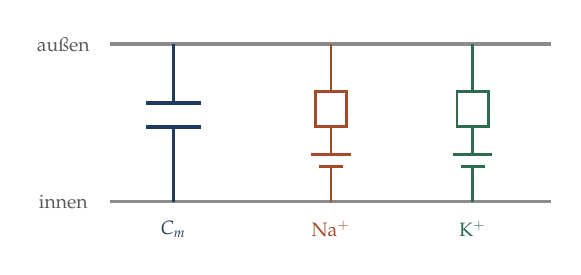
\begin{tikzpicture}[scale=1.0]
\draw[grau!70, line width=1.2pt] (-2.6,1.0) -- (3.0,1.0);
\draw[grau!70, line width=1.2pt] (-2.6,-1.0) -- (3.0,-1.0);
\node[font=\scriptsize, color=grau] at (-3.2,1.0) {außen};
\node[font=\scriptsize, color=grau] at (-3.2,-1.0) {innen};
% Kondensator
\draw[tief, line width=1.0pt] (-1.8,1.0) -- (-1.8,0.25);
\draw[tief, line width=1.4pt] (-2.15,0.25) -- (-1.45,0.25);
\draw[tief, line width=1.4pt] (-2.15,-0.05) -- (-1.45,-0.05);
\draw[tief, line width=1.0pt] (-1.8,-0.05) -- (-1.8,-1.0);
\node[font=\scriptsize, color=tief] at (-1.8,-1.35) {$C_m$};
% Kanal Na
\draw[akzent, line width=1.0pt] (0.2,1.0) -- (0.2,0.4);
\draw[akzent, line width=1.0pt] (0.0,0.4) rectangle (0.4,-0.05);
\draw[akzent, line width=1.0pt] (0.2,-0.05) -- (0.2,-0.4);
\draw[akzent, line width=1.3pt] (-0.05,-0.4) -- (0.45,-0.4);
\draw[akzent, line width=1.0pt] (0.05,-0.55) -- (0.35,-0.55);
\draw[akzent, line width=1.0pt] (0.2,-0.55) -- (0.2,-1.0);
\node[font=\scriptsize, color=akzent] at (0.2,-1.35) {Na$^+$};
% Kanal K
\draw[gruen, line width=1.0pt] (2.0,1.0) -- (2.0,0.4);
\draw[gruen, line width=1.0pt] (1.8,0.4) rectangle (2.2,-0.05);
\draw[gruen, line width=1.0pt] (2.0,-0.05) -- (2.0,-0.4);
\draw[gruen, line width=1.3pt] (1.75,-0.4) -- (2.25,-0.4);
\draw[gruen, line width=1.0pt] (1.85,-0.55) -- (2.15,-0.55);
\draw[gruen, line width=1.0pt] (2.0,-0.55) -- (2.0,-1.0);
\node[font=\scriptsize, color=gruen] at (2.0,-1.35) {K$^+$};
\end{tikzpicture}
\end{center}
\end{merksatz}

\begin{merksatz}
\boxtitel{Die Nernst-Spannung}
Für jede Ionenart stellt sich eine Spannung ein, bei der Diffusion und elektrische Kraft einander aufheben:
\[ E = \frac{R\,T}{z\,F}\,\ln\frac{c_{\text{außen}}}{c_{\text{innen}}} \;\approx\; \frac{61{,}5\ \mathrm{mV}}{z}\,\lg\frac{c_{\text{außen}}}{c_{\text{innen}}} \]
bei Körpertemperatur.

\begin{center}
{\small
\renewcommand{\arraystretch}{1.45}
\begin{tabular}{@{}P{1.6cm}P{1.8cm}P{1.8cm}P{2.0cm}@{}}
\toprule
\textbf{Ion} & \textbf{außen} & \textbf{innen} & $E$\\
\midrule
K$^+$ & $5$ & $140$ & $-89$ mV\\
Na$^+$ & $145$ & $15$ & $+61$ mV\\
Cl$^-$ & $110$ & $10$ & $-64$ mV\\
Ca$^{2+}$ & $2$ & $0{,}0001$ & $+132$ mV\\
\bottomrule
\end{tabular}}
\end{center}
\kursiv{Konzentrationen in mmol/l.}

\begin{center}
\begin{minipage}{0.88\textwidth}
\kursiv{Die Ruhespannung von etwa $-70$ mV liegt nahe bei $E_K$, weil die Membran in Ruhe überwiegend für Kalium durchlässig ist. Öffnen sich Natriumkanäle, so wandert die Spannung in Richtung $+61$ mV --- das ist der Aufstrich des Aktionspotentials.}
\end{minipage}
\end{center}
\end{merksatz}

\section{Die passive Membran}

\begin{merksatz}
\boxtitel{Satz 12.1 --- die Zeitkonstante}
Bleiben die Leitfähigkeiten fest, so gilt für die Spannung $V$ bei einem eingeprägten Strom $I$
\[ C_m\frac{\dd V}{\dd t} = -\frac{V - E}{R_m} + I \]
mit der Lösung
\[ V(t) = V_\infty + (V_0 - V_\infty)\,e^{-t/\tau}, \qquad \tau = R_m\,C_m . \]

\schritt{Beweis}
Umformen:
\[ \frac{\dd V}{\dd t} = -\frac{1}{R_mC_m}\bigl(V - E - R_mI\bigr) = -\frac{1}{\tau}\bigl(V - V_\infty\bigr) \]
mit $V_\infty := E + R_mI$.

Das ist die Anflutungsgleichung aus Satz 10.2, nur mit einem anderen Ausgangswert. Trennung der Veränderlichen wie dort. $\blacksquare$

\schritt{Die Zahlen}
Mit $C_m = 1\ \mathrm{\mu F/cm^2}$ und $R_m = 10\ \mathrm{k\Omega\,cm^2}$:
\[ \tau = 10^4\,\Omega\,\mathrm{cm^2} \cdot 10^{-6}\,\mathrm{F/cm^2} = 10^{-2}\,\mathrm{s} = 10\ \mathrm{ms} \]

\begin{center}
\begin{minipage}{0.88\textwidth}
\kursiv{Wieder die Vier-Zeitkonstanten-Regel aus Kapitel~10: Nach $40$ ms ist die passive Antwort praktisch abgeschlossen. Und wieder gilt --- die Zeitkonstante hängt nicht von der Reizstärke ab, nur der Endwert tut es.}
\end{minipage}
\end{center}

\schritt{Was die passive Membran nicht kann}
Sie antwortet stets \kursiv{proportional} zum Reiz. Ein doppelt so starker Reiz erzeugt eine doppelt so große Antwort. Ein Schwellenverhalten gibt es nicht.

\begin{center}
\begin{minipage}{0.9\textwidth}
\textbf{Alles-oder-Nichts verlangt, dass die Leitfähigkeiten selbst von der Spannung abhängen.} Damit wird die Gleichung nichtlinear --- und alles Weitere möglich.
\end{minipage}
\end{center}
\end{merksatz}

\section{Das Modell von Hodgkin und Huxley}

\begin{merksatz}
\boxtitel{Die Idee in vier Gleichungen}
\[ C_m\frac{\dd V}{\dd t} = -\bar{g}_{\mathrm{Na}}m^3h\,(V-E_{\mathrm{Na}}) - \bar{g}_{\mathrm{K}}n^4\,(V-E_{\mathrm{K}}) - g_L(V-E_L) + I \]
dazu drei Gleichungen der Form
\[ \frac{\dd m}{\dd t} = \frac{m_\infty(V) - m}{\tau_m(V)} \]
für $m$, $h$ und $n$.

\begin{center}
{\small
\renewcommand{\arraystretch}{1.5}
\begin{tabular}{@{}P{1.4cm}P{2.6cm}P{4.0cm}@{}}
\toprule
$m$ & Natrium-Aktivierung & öffnet \kursiv{schnell} bei Depolarisation\\
$h$ & Natrium-Inaktivierung & schließt \kursiv{langsam} bei Depolarisation\\
$n$ & Kalium-Aktivierung & öffnet \kursiv{langsam}\\
\bottomrule
\end{tabular}}
\end{center}

\schritt{Der Ablauf eines Aktionspotentials}
\begin{center}
\renewcommand{\arraystretch}{1.5}
\begin{tabular}{@{}P{1.0cm}P{7.4cm}@{}}
\toprule
$1$ & Reiz hebt $V$ an; $m$ öffnet rasch; Natrium strömt ein.\\
$2$ & Einströmendes Natrium hebt $V$ weiter --- \textbf{positive Rückkopplung}, der Aufstrich.\\
$3$ & Verzögert schließt $h$ und öffnet $n$; Natrium versiegt, Kalium strömt aus.\\
$4$ & $V$ fällt, teils unter die Ruhespannung. Erholung.\\
\bottomrule
\end{tabular}
\end{center}

\begin{center}
\begin{minipage}{0.88\textwidth}
\kursiv{In Schritt 2 steckt die Erklärung des Alles-oder-Nichts: Die positive Rückkopplung springt erst an, wenn genug Natriumkanäle offen sind. Unterhalb der Schwelle überwiegt der Kaliumstrom und zieht die Spannung zurück.}
\end{minipage}
\end{center}

\schritt{Warum wir es nicht ausrechnen}
Vier gekoppelte Gleichungen mit spannungsabhängigen Koeffizienten lassen sich nicht von Hand lösen. Hodgkin und Huxley rechneten 1952 an einer Handkurbelmaschine; eine einzige Kurve kostete Wochen.

\begin{center}
\begin{minipage}{0.88\textwidth}
\kursiv{Für das \kursiv{Verstehen} ist das auch nicht nötig. Der nächste Abschnitt zeigt ein Modell mit zwei Gleichungen, das dasselbe Verhalten erzeugt und sich mit den Werkzeugen aus Kapitel~6 vollständig durchschauen lässt.}
\end{minipage}
\end{center}
\end{merksatz}

\section{Das Modell von FitzHugh und Nagumo}

\begin{definition}
\boxtitelm{Definition 12.2}
\[ \frac{\dd v}{\dd t} = v - \frac{v^3}{3} - w + I, \qquad \frac{\dd w}{\dd t} = \varepsilon\,(v + a - b\,w) \]
mit $\varepsilon$ klein. Wir rechnen mit $a=0{,}7$, $b=0{,}8$, $\varepsilon=0{,}08$.
\end{definition}

\begin{merksatz}
\boxtitel{Was die beiden Größen bedeuten}
\begin{center}
{\small
\renewcommand{\arraystretch}{1.5}
\begin{tabular}{@{}P{1.4cm}P{2.8cm}P{3.8cm}@{}}
\toprule
$v$ & Spannung & ändert sich \kursiv{schnell}\\
$w$ & Erholung & ändert sich \kursiv{langsam} --- daher $\varepsilon$ klein\\
$I$ & eingeprägter Strom & der Reiz\\
\bottomrule
\end{tabular}}
\end{center}

\schritt{Woher die Bauteile stammen}
\begin{center}
\renewcommand{\arraystretch}{1.5}
\begin{tabular}{@{}P{2.4cm}P{6.2cm}@{}}
\toprule
$v - v^3/3$ & Die kubische Form erzeugt einen Bereich, in dem $\dd v/\dd t$ mit $v$ \kursiv{wächst} --- die positive Rückkopplung.\\
$-w$ & Die Erholung bremst.\\
$\varepsilon$ & Die Erholung kommt verzögert --- die Ursache aller Schwingungen, wie in Kapitel~3.\\
\bottomrule
\end{tabular}
\end{center}
\end{merksatz}

\begin{merksatz}
\boxtitel{Die Nullklinen}
\begin{center}
\renewcommand{\arraystretch}{1.5}
\begin{tabular}{@{}P{2.0cm}P{6.4cm}@{}}
\toprule
$v$-Nullkline & $w = v - \dfrac{v^3}{3} + I$ --- eine \kursiv{kubische} Kurve mit $N$-Form\\
$w$-Nullkline & $w = \dfrac{v+a}{b}$ --- eine Gerade\\
\bottomrule
\end{tabular}
\end{center}

\begin{center}
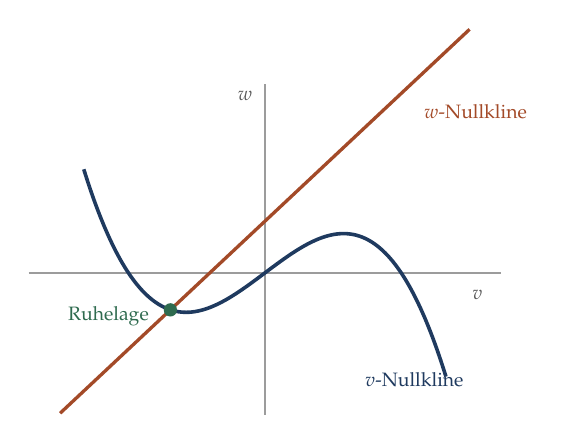
\begin{tikzpicture}[scale=1.0]
\draw[grau!60, line width=0.7pt] (-3.0,0) -- (3.0,0);
\draw[grau!60, line width=0.7pt] (0,-1.8) -- (0,2.4);
\draw[tief, line width=1.3pt, smooth, samples=70, domain=-2.3:2.3]
  plot (\x, {0.75*(\x - \x*\x*\x/3)});
\draw[akzent, line width=1.2pt] (-2.6,{0.75*(-2.6+0.7)/0.8}) -- (2.6,{0.75*(2.6+0.7)/0.8});
\fill[gruen] (-1.2,{0.75*(-1.2+0.7)/0.8}) circle (2.4pt);
\node[font=\scriptsize, color=tief, anchor=west] at (1.15,-1.35) {$v$-Nullkline};
\node[font=\scriptsize, color=akzent, anchor=west] at (1.9,2.05) {$w$-Nullkline};
\node[font=\scriptsize, color=gruen, anchor=east] at (-1.35,-0.55) {Ruhelage};
\node[font=\scriptsize, color=grau] at (2.7,-0.28) {$v$};
\node[font=\scriptsize, color=grau] at (-0.25,2.25) {$w$};
\end{tikzpicture}
\end{center}

\begin{center}
\begin{minipage}{0.88\textwidth}
\kursiv{Entscheidend ist, \kursiv{wo} die Gerade die Kurve schneidet. Schneidet sie den äußeren, fallenden Ast, so ist der Punkt stabil --- die Zelle ruht. Schneidet sie den mittleren, steigenden Ast, so ist er instabil --- und die Zelle feuert dauernd.}
\end{minipage}
\end{center}
\end{merksatz}

\begin{merksatz}
\boxtitel{Die Stabilität, mit den Werkzeugen aus Kapitel 6}
\schritt{Die Jacobi-Matrix}
\[ \frac{\partial f}{\partial v} = 1 - v^2, \qquad \frac{\partial f}{\partial w} = -1 \]
\[ \frac{\partial g}{\partial v} = \varepsilon, \qquad \frac{\partial g}{\partial w} = -\varepsilon b \]

\schritt{Spur und Determinante}
\[ T = (1-v^{*2}) - \varepsilon b \]
\[ D = (1-v^{*2})(-\varepsilon b) - (-1)(\varepsilon) = \varepsilon\bigl(1 - b(1-v^{*2})\bigr) \]

\schritt{Ohne Reiz --- $I = 0$}
Die Ruhelage liegt bei $v^{*} = -1{,}1994$, $w^{*} = -0{,}6243$.
\[ 1 - v^{*2} = 1 - 1{,}4386 = -0{,}4386 \]
\[ T = -0{,}4386 - 0{,}064 = -0{,}5026 \]
\[ D = (-0{,}4386)(-0{,}064) + 0{,}08 = 0{,}0281 + 0{,}08 = 0{,}1081 \]
\[ T^2 - 4D = 0{,}2526 - 0{,}4323 = -0{,}1797 < 0 \]

$T<0$, $D>0$, Diskriminante negativ: \textbf{stabiler Strudel.} Die Zelle ruht.
\end{merksatz}

\begin{merksatz}
\boxtitel{Satz 12.3 --- wann die Zelle zu feuern beginnt}
Die Ruhelage verliert ihre Stabilität genau dann, wenn
\[ v^{*2} = 1 - \varepsilon\,b . \]

\schritt{Beweis}
Nach Satz 6.3 ist der Punkt stabil, solange $T<0$ und $D>0$. Die Determinante
\[ D = \varepsilon\bigl(1-b(1-v^{*2})\bigr) \]
ist bei unseren Werten stets positiv. Entscheidend ist also $T$:
\[ T = 0 \quad\Longleftrightarrow\quad 1-v^{*2} = \varepsilon b \quad\Longleftrightarrow\quad v^{*2} = 1-\varepsilon b . \qquad \blacksquare \]

\schritt{Die Zahlen}
\[ v^{*} = \pm\sqrt{1 - 0{,}08 \cdot 0{,}8} = \pm\sqrt{0{,}936} = \pm 0{,}9675 \]

Das sind genau die Punkte, an denen die kubische Kurve ihre Scheitel hat --- denn dort ist $1-v^2 \approx 0$.

\schritt{Die zugehörigen Reizströme}
Aus der $v$-Nullkline $I = w - v + v^3/3$ mit $w = (v+a)/b$:
\begin{center}
\renewcommand{\arraystretch}{1.48}
\begin{tabular}{@{}P{2.0cm}P{2.0cm}P{2.6cm}@{}}
\toprule
$v^{*}$ & $w^{*}$ & $I$\\
\midrule
$-0{,}9675$ & $-0{,}3343$ & $\mathbf{0{,}331}$\\
$+0{,}9675$ & $+2{,}0843$ & $\mathbf{1{,}419}$\\
\bottomrule
\end{tabular}
\end{center}

\begin{center}
\begin{minipage}{0.9\textwidth}
\textbf{Für $0{,}331 < I < 1{,}419$ feuert die Zelle dauernd. Außerhalb ruht sie.}
\end{minipage}
\end{center}
\end{merksatz}

\begin{merksatz}
\boxtitel{Der Übergang in Zahlen}
\begin{center}
{\small
\renewcommand{\arraystretch}{1.45}
\begin{tabular}{@{}P{1.4cm}P{1.8cm}P{1.8cm}P{1.6cm}P{1.8cm}@{}}
\toprule
$I$ & $v^{*}$ & $T$ & $D$ & \textbf{Zustand}\\
\midrule
$0{,}0$ & $-1{,}199$ & $-0{,}503$ & $0{,}108$ & \textcolor{gruen}{Ruhe}\\
$0{,}2$ & $-1{,}069$ & $-0{,}208$ & $0{,}089$ & \textcolor{gruen}{Ruhe}\\
$0{,}3$ & $-0{,}993$ & $-0{,}051$ & $0{,}079$ & \textcolor{gruen}{Ruhe}\\
$\mathbf{0{,}331}$ & $-0{,}968$ & $\mathbf{0{,}000}$ & $0{,}076$ & \textcolor{akzent}{\textbf{Hopf}}\\
$0{,}4$ & $-0{,}907$ & $+0{,}114$ & $0{,}069$ & \textcolor{akzent}{Dauerfeuer}\\
$1{,}0$ & $+0{,}409$ & $+0{,}769$ & $0{,}027$ & \textcolor{akzent}{Dauerfeuer}\\
$\mathbf{1{,}419}$ & $+0{,}968$ & $\mathbf{0{,}000}$ & $0{,}076$ & \textcolor{akzent}{\textbf{Hopf}}\\
$1{,}8$ & $+1{,}228$ & $-0{,}573$ & $0{,}113$ & \textcolor{gruen}{Ruhe}\\
\bottomrule
\end{tabular}}
\end{center}

\begin{center}
\begin{minipage}{0.9\textwidth}
\textbf{Das ist die Hopf-Bifurkation aus Kapitel~6, an einem biologischen Beispiel.} Der Punkt $(T,D)$ wandert über die senkrechte Achse des Diagramms --- und aus Ruhe wird Schwingung.
\end{minipage}
\end{center}

\schritt{Die zweite Schwelle ist bemerkenswert}
Bei sehr starkem Reiz hört die Zelle wieder auf zu feuern und verharrt in einem dauerhaft erregten Zustand.

\begin{center}
\begin{minipage}{0.88\textwidth}
\kursiv{Das ist keine Eigenart des Modells, sondern beobachtbar: Man nennt es \Begriff{Depolarisationsblock}. Er tritt bei sehr starker Reizung auf --- und ist der vermutete Wirkmechanismus mehrerer Arzneistoffe, die auf Nervenzellen dämpfend wirken.}
\end{minipage}
\end{center}
\end{merksatz}

\section{Erregbarkeit}

\begin{merksatz}
\boxtitel{Wie die Schwelle ohne Schwellenwert entsteht}
Bei $I=0$ ist die Ruhelage stabil --- jede Störung klingt ab. Trotzdem gibt es ein Alles-oder-Nichts.

\schritt{Der Grund}
Der Weg zurück zur Ruhelage kann auf zwei völlig verschiedenen Wegen verlaufen:

\begin{center}
{\small
\renewcommand{\arraystretch}{1.5}
\begin{tabular}{@{}P{2.4cm}P{6.2cm}@{}}
\toprule
\textbf{Kleine Störung} & $v$ bleibt links vom mittleren Ast. Die Bahn läuft unmittelbar zur Ruhelage zurück.\\
\textbf{Große Störung} & $v$ überschreitet den mittleren Ast. Die Bahn wird nach rechts auf den anderen Ast gerissen, läuft ihn hinauf, springt zurück --- ein voller Ausschlag.\\
\bottomrule
\end{tabular}}
\end{center}

\begin{center}
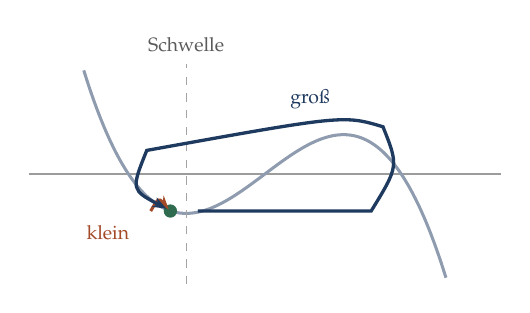
\begin{tikzpicture}[scale=1.0]
\draw[grau!60, line width=0.7pt] (-3.0,0) -- (3.0,0);
\draw[tief!50, line width=1.1pt, smooth, samples=70, domain=-2.3:2.3]
  plot (\x, {0.75*(\x - \x*\x*\x/3)});
\fill[gruen] (-1.2,-0.47) circle (2.4pt);
\draw[grau!55, dashed] (-1.0,-1.4) -- (-1.0,1.4);
\node[font=\scriptsize, color=grau] at (-1.0,1.65) {Schwelle};
\draw[akzent, line width=1.1pt, -{Stealth[length=5pt]}] (-1.45,-0.47) .. controls (-1.35,-0.3) .. (-1.22,-0.45);
\draw[tief, line width=1.2pt, -{Stealth[length=5pt]}]
  (-0.85,-0.47) -- (1.35,-0.47) .. controls (1.7,0.1) .. (1.5,0.6)
  .. controls (1.0,0.75) .. (-1.5,0.3) .. controls (-1.7,-0.2) .. (-1.25,-0.44);
\node[font=\scriptsize, color=akzent, anchor=east] at (-1.6,-0.75) {klein};
\node[font=\scriptsize, color=tief, anchor=west] at (0.2,0.95) {groß};
\end{tikzpicture}
\end{center}

\begin{center}
\begin{minipage}{0.9\textwidth}
\textbf{Es gibt keinen Schwellenwert in den Gleichungen.} Die Schwelle entsteht aus der Form der kubischen Nullkline --- aus der Lage des mittleren, abstoßenden Astes.
\end{minipage}
\end{center}

\begin{center}
\begin{minipage}{0.88\textwidth}
\kursiv{Das ist die Antwort auf die Frage aus Abschnitt 12.1. Ein Schaltverhalten braucht keinen Schalter. Es genügt, dass zwei Vorgänge verschieden schnell ablaufen und einer von ihnen sich selbst verstärkt.}
\end{minipage}
\end{center}
\end{merksatz}

\begin{merksatz}
\boxtitel{Und die Refraktärzeit}
Nach einem Ausschlag ist $w$ erhöht --- die Erholungsgröße. Solange sie nicht abgebaut ist, liegt die Bahn oberhalb, und die Schwelle ist weiter rechts.

\begin{center}
\renewcommand{\arraystretch}{1.5}
\begin{tabular}{@{}P{2.6cm}P{6.0cm}@{}}
\toprule
\textbf{Absolut} & Unmittelbar danach ist kein Ausschlag möglich, gleichgültig wie stark gereizt wird.\\
\textbf{Relativ} & Etwas später ist einer möglich, aber nur bei stärkerem Reiz.\\
\bottomrule
\end{tabular}
\end{center}

\begin{center}
\begin{minipage}{0.88\textwidth}
\kursiv{Beide Formen fallen im Modell ab, ohne eigens eingebaut zu sein. Die Refraktärzeit ist der Grund, warum die Erregung im Axon nur in eine Richtung läuft --- rückwärts trifft sie auf frisch erregtes, unerregbares Gewebe.}
\end{minipage}
\end{center}
\end{merksatz}

\section{Der Bruchfall}

\begin{warnung}
\boxtitelr{Was FitzHugh-Nagumo nicht kann}
\begin{center}
{\small
\renewcommand{\arraystretch}{1.5}
\begin{tabular}{@{}P{2.4cm}P{6.2cm}@{}}
\toprule
\textbf{Keine Ionen} & $v$ und $w$ haben keine unmittelbare stoffliche Bedeutung. Man kann keine Wirkung eines Kanalblockers vorhersagen.\\
\textbf{Keine Amplituden} & Die Größe des Ausschlags ist eine Modellgröße, keine Spannung in Millivolt.\\
\textbf{Ein Raumpunkt} & Die Ausbreitung entlang eines Axons fehlt; dafür braucht man eine Gleichung mit Ortsableitung.\\
\bottomrule
\end{tabular}}
\end{center}

\begin{center}
\begin{minipage}{0.9\textwidth}
\textbf{Das Modell erklärt, \kursiv{warum} es ein Alles-oder-Nichts gibt. Es sagt nicht vorher, \kursiv{wie} die Zelle auf einen bestimmten Stoff reagiert.}
\end{minipage}
\end{center}

\begin{center}
\begin{minipage}{0.88\textwidth}
\kursiv{Damit ist die Arbeitsteilung benannt, die dieses Kapitel trägt: Hodgkin-Huxley ist das Modell für Vorhersagen, FitzHugh-Nagumo das Modell für Einsicht. Beide sind nötig, und keines ersetzt das andere.}
\end{minipage}
\end{center}
\end{warnung}

\begin{warnung}
\boxtitelr{Und was auch Hodgkin-Huxley nicht leistet}
\begin{center}
{\small
\renewcommand{\arraystretch}{1.5}
\begin{tabular}{@{}P{2.6cm}P{6.0cm}@{}}
\toprule
\textbf{Stetige Größen} & $m$, $h$ und $n$ sind Anteile offener Kanäle. Bei wenigen Kanälen ist das Öffnen zufällig --- die Zelle feuert dann gelegentlich spontan.\\
\textbf{Eine Zellart} & Die Parameter stammen vom Riesenaxon des Tintenfischs. Andere Zellen haben andere Kanäle und völlig anderes Verhalten.\\
\textbf{Feste Parameter} & Kanaldichten ändern sich über Stunden bis Tage --- die Zelle regelt ihre eigene Erregbarkeit.\\
\bottomrule
\end{tabular}}
\end{center}

\begin{center}
\begin{minipage}{0.88\textwidth}
\kursiv{Die letzte Zeile ist ein Forschungsfeld für sich: Nervenzellen halten ihre Feuerrate über lange Zeit in einem Zielbereich, indem sie die Zahl ihrer Kanäle anpassen. Das ist eine Rückkopplung auf einer viel langsameren Zeitskala --- und Modelle, die sie einbauen, erklären, warum sehr verschiedene Kanalausstattungen dasselbe Verhalten erzeugen können.}
\end{minipage}
\end{center}
\end{warnung}

\section{Übungsaufgaben}

\begin{aufgabe}
\boxtitel{Aufgabe 12.1 --- Nernst-Spannungen und Ruhepotential}
Berechnen Sie $E_K$ und $E_{\mathrm{Na}}$ für die Werte aus Abschnitt 12.1 und bestimmen Sie die Ruhespannung, wenn die Kaliumleitfähigkeit $25$-mal so groß ist wie die Natriumleitfähigkeit.

\loesung
\schritt{Schritt 1 --- Die Nernst-Spannungen}
\[ E_K = 61{,}5 \cdot \lg\frac{5}{140} = 61{,}5 \cdot \lg 0{,}03571 = 61{,}5 \cdot (-1{,}4472) = -89{,}0\ \mathrm{mV} \]
\[ E_{\mathrm{Na}} = 61{,}5 \cdot \lg\frac{145}{15} = 61{,}5 \cdot \lg 9{,}667 = 61{,}5 \cdot 0{,}9853 = +60{,}6\ \mathrm{mV} \]

\schritt{Schritt 2 --- Die Ruhespannung}
Im Ruhezustand ist der Gesamtstrom null:
\[ g_K(V-E_K) + g_{\mathrm{Na}}(V-E_{\mathrm{Na}}) = 0 \]
\[ V\,(g_K+g_{\mathrm{Na}}) = g_KE_K + g_{\mathrm{Na}}E_{\mathrm{Na}} \]
\[ V = \frac{g_KE_K + g_{\mathrm{Na}}E_{\mathrm{Na}}}{g_K+g_{\mathrm{Na}}} \]

\begin{center}
\begin{minipage}{0.88\textwidth}
\kursiv{Die Ruhespannung ist also ein mit den Leitfähigkeiten \kursiv{gewichtetes Mittel} der Nernst-Spannungen --- dieselbe Rechenfigur wie beim Simpson-Paradoxon in Band 17, Kapitel~3.}
\end{minipage}
\end{center}

\schritt{Schritt 3 --- Einsetzen}
Mit $g_K = 25\,g_{\mathrm{Na}}$:
\[ V = \frac{25 \cdot (-89{,}0) + 1 \cdot 60{,}6}{26} = \frac{-2225 + 60{,}6}{26} = \frac{-2164{,}4}{26} = -83{,}2\ \mathrm{mV} \]

\schritt{Schritt 4 --- Die Empfindlichkeit}
\begin{center}
\renewcommand{\arraystretch}{1.45}
\begin{tabular}{@{}P{2.4cm}P{2.4cm}P{2.6cm}@{}}
\toprule
$g_K/g_{\mathrm{Na}}$ & $V$ & \\
\midrule
$100$ & $-87{,}5$ mV & sehr nahe an $E_K$\\
$25$ & $-83{,}2$ mV & \\
$10$ & $-75{,}4$ mV & \\
$1$ & $-14{,}2$ mV & \\
$0{,}1$ & $+47{,}0$ mV & nahe an $E_{\mathrm{Na}}$\\
\bottomrule
\end{tabular}
\end{center}

\schritt{Schritt 5 --- Die Deutung}
\begin{center}
\begin{minipage}{0.9\textwidth}
\textbf{Die Spannung folgt stets derjenigen Ionenart, für die die Membran gerade am durchlässigsten ist.}
\end{minipage}
\end{center}

\begin{center}
\begin{minipage}{0.88\textwidth}
\kursiv{Das ist der ganze Mechanismus des Aktionspotentials: Öffnen sich die Natriumkanäle, so kehrt sich das Verhältnis kurzzeitig um, und die Spannung springt Richtung $+60$ mV. Schließen sie wieder und öffnen die Kaliumkanäle, so fällt sie zurück --- vorübergehend sogar unter die Ruhespannung, weil das Verhältnis dann noch günstiger für Kalium ist als in Ruhe.}
\end{minipage}
\end{center}

\schritt{Schritt 6 --- Eine klinische Anwendung}
Steigt die äußere Kaliumkonzentration von $5$ auf $8$ mmol/l:
\[ E_K = 61{,}5 \cdot \lg\frac{8}{140} = 61{,}5 \cdot (-1{,}2430) = -76{,}4\ \mathrm{mV} \]
\[ V = \frac{25 \cdot (-76{,}4) + 60{,}6}{26} = \frac{-1910 + 60{,}6}{26} = -71{,}1\ \mathrm{mV} \]

Die Zelle wird um $12$ mV depolarisiert --- näher an die Schwelle.

\begin{center}
\begin{minipage}{0.86\textwidth}
\kursiv{Daher die Gefährlichkeit einer erhöhten Kaliumkonzentration im Blut: Die Zellen liegen näher an der Schwelle und werden zunächst übererregbar, bei weiterem Anstieg dann unerregbar --- der Depolarisationsblock aus Abschnitt 12.4. Am Herzen ist das lebensbedrohlich.}
\end{minipage}
\end{center}
\end{aufgabe}

\begin{aufgabe}
\boxtitel{Aufgabe 12.2 --- Die Feuerschwelle verschieben}
Wie ändert sich der Bereich des Dauerfeuers, wenn $\varepsilon$ von $0{,}08$ auf $0{,}3$ steigt? Deuten Sie das Ergebnis.

\loesung
\schritt{Schritt 1 --- Die Bedingung}
Nach Satz 12.3 liegt die Hopf-Bifurkation bei
\[ v^{*2} = 1 - \varepsilon b \]

\schritt{Schritt 2 --- Die beiden Fälle}
\[ \varepsilon = 0{,}08: \quad v^{*} = \pm\sqrt{1-0{,}064} = \pm 0{,}9675 \]
\[ \varepsilon = 0{,}30: \quad v^{*} = \pm\sqrt{1-0{,}24} = \pm\sqrt{0{,}76} = \pm 0{,}8718 \]

\schritt{Schritt 3 --- Die zugehörigen Ströme}
Mit $I = \frac{v+a}{b} - v + \frac{v^3}{3}$:

\kursiv{Für $v = -0{,}8718$:}
\[ w = \frac{-0{,}8718+0{,}7}{0{,}8} = -0{,}2148 \]
\[ v^3/3 = \frac{-0{,}6626}{3} = -0{,}2209 \]
\[ I = -0{,}2148 + 0{,}8718 - 0{,}2209 = 0{,}4361 \]

\kursiv{Für $v = +0{,}8718$:}
\[ w = \frac{1{,}5718}{0{,}8} = 1{,}9648, \qquad I = 1{,}9648 - 0{,}8718 + 0{,}2209 = 1{,}3139 \]

\schritt{Schritt 4 --- Der Vergleich}
\begin{center}
\renewcommand{\arraystretch}{1.48}
\begin{tabular}{@{}P{1.8cm}P{2.0cm}P{2.0cm}P{2.0cm}@{}}
\toprule
$\varepsilon$ & \textbf{unten} & \textbf{oben} & \textbf{Breite}\\
\midrule
$0{,}08$ & $0{,}331$ & $1{,}419$ & $1{,}088$\\
$0{,}30$ & $0{,}436$ & $1{,}314$ & $0{,}878$\\
\bottomrule
\end{tabular}
\end{center}

\schritt{Schritt 5 --- Die Deutung}
\begin{center}
\begin{minipage}{0.9\textwidth}
\textbf{Eine schnellere Erholung verengt den Bereich des Dauerfeuers von beiden Seiten.}
\end{minipage}
\end{center}

Der Grund: $w$ folgt der Spannung rascher und bremst früher. Die verzögerte Rückkopplung, die das Schwingen erzeugt, wird schwächer.

\begin{center}
\begin{minipage}{0.88\textwidth}
\kursiv{Bei $\varepsilon b > 1$ --- also $\varepsilon > 1{,}25$ --- verschwindet der Bereich ganz: Dann hat $v^{*2} = 1-\varepsilon b$ keine reelle Lösung, und die Ruhelage ist für \kursiv{jeden} Strom stabil. Die Zelle wäre dann nicht mehr erregbar. Das ist der rechnerische Kern dessen, was ein dämpfender Wirkstoff bewirkt.}
\end{minipage}
\end{center}

\schritt{Schritt 6 --- Der Grenzwert}
\[ \varepsilon_c = \frac{1}{b} = \frac{1}{0{,}8} = 1{,}25 \]

\kursiv{Probe bei $\varepsilon = 1{,}25$:} $v^{*2} = 1 - 1{,}25\cdot0{,}8 = 0$, also $v^{*} = 0$ --- die beiden Bifurkationspunkte fallen zusammen und verschwinden danach. \checkmark
\end{aufgabe}

\begin{aufgabe}
\boxtitel{Aufgabe 12.3 --- Die passive Antwort}
Eine Zelle mit $\tau = 10$ ms und Ruhespannung $-70$ mV erhält einen Strom, der die Spannung auf $-50$ mV treiben würde. Die Schwelle liegt bei $-55$ mV. Wird die Zelle erregt --- und wann?

\loesung
\schritt{Schritt 1 --- Die Lösung aufstellen}
Nach Satz 12.1:
\[ V(t) = V_\infty + (V_0-V_\infty)\,e^{-t/\tau} = -50 + (-70+50)\,e^{-t/10} = -50 - 20\,e^{-t/10} \]
mit $t$ in Millisekunden.

\schritt{Schritt 2 --- Die Probe}
\[ V(0) = -50 - 20 = -70 \quad \checkmark \qquad V(\infty) = -50 \quad \checkmark \]

\schritt{Schritt 3 --- Wann die Schwelle erreicht wird}
\[ -55 = -50 - 20\,e^{-t/10} \]
\[ -5 = -20\,e^{-t/10} \quad\Longrightarrow\quad e^{-t/10} = 0{,}25 \]
\[ -\frac{t}{10} = \ln 0{,}25 = -1{,}386 \quad\Longrightarrow\quad t = 13{,}86\ \mathrm{ms} \]

\textbf{Ja, nach knapp $14$ ms.}

\schritt{Schritt 4 --- Die Kontrolle in Zeitkonstanten}
Von $-70$ auf $-50$ ist die Spanne $20$ mV; bis $-55$ sind $15$ mV zurückzulegen, also $75\,\%$. Nach der Tabelle aus Kapitel~10 entspricht das genau zwei Zeitkonstanten:
\[ t = 2 \cdot 10 = 20\ \mathrm{ms}\ ? \]

Das stimmt nicht. Prüfen wir: $1 - e^{-2} = 0{,}865$, also $86{,}5\,\%$. Zwei Zeitkonstanten wären zu viel.

\kursiv{Richtig:} $75\,\%$ entspricht $e^{-t/\tau} = 0{,}25$, also $t/\tau = \ln 4 = 1{,}386$. \checkmark

\begin{center}
\begin{minipage}{0.86\textwidth}
\kursiv{Die Verwechslung ist lehrreich: $75\,\%$ ist der Wert nach \kursiv{zwei Halbwertszeiten}, nicht nach zwei Zeitkonstanten. Es gilt $t_{1/2} = \tau\ln 2 = 6{,}93$ ms. Zeitkonstante und Halbwertszeit unterscheiden sich um den Faktor $\ln 2$ --- ein Fehler, der leicht unterläuft.}
\end{minipage}
\end{center}

\schritt{Schritt 5 --- Ein schwächerer Reiz}
Würde der Strom die Spannung nur auf $-58$ mV treiben:
\[ V(t) = -58 - 12\,e^{-t/10} \]
Der Endwert $-58$ liegt \kursiv{unter} der Schwelle $-55$. Die Zelle wird nie erregt, gleichgültig wie lange gereizt wird.

\begin{center}
\begin{minipage}{0.9\textwidth}
\textbf{Es gibt eine Mindeststromstärke, unterhalb derer keine Erregung möglich ist} --- die \Begriff{Rheobase}.
\end{minipage}
\end{center}

\schritt{Schritt 6 --- Die Strom-Zeit-Beziehung}
Aus der Lösung folgt allgemein: Ist $V_\infty$ um den Faktor $q > 1$ über der Schwelle, so wird sie erreicht bei
\[ t = \tau\,\ln\frac{q}{q-1} . \]

\begin{center}
\renewcommand{\arraystretch}{1.45}
\begin{tabular}{@{}P{2.6cm}P{2.2cm}P{2.4cm}@{}}
\toprule
\textbf{Reiz} & $q$ & \textbf{Zeit}\\
\midrule
knapp über Rheobase & $1{,}1$ & $24{,}0$ ms\\
$1{,}33$-fach & $1{,}33$ & $13{,}9$ ms\\
doppelt & $2$ & $6{,}9$ ms\\
vierfach & $4$ & $2{,}9$ ms\\
\bottomrule
\end{tabular}
\end{center}

\begin{center}
\begin{minipage}{0.88\textwidth}
\kursiv{Diese Beziehung zwischen Reizstärke und nötiger Reizdauer wird in der Neurologie gemessen und heißt \kursiv{Reizzeit-Spannungs-Kurve}. Die Zeit bei doppelter Rheobase --- hier $6{,}9$ ms --- heißt \Begriff{Chronaxie} und ist eine Kennzahl der Erregbarkeit. Sie beträgt genau $\tau\ln 2$, also die Halbwertszeit der Membran.}
\end{minipage}
\end{center}
\end{aufgabe}

\begin{geschichte}
\boxtitelg{Ein Tintenfisch und zwei Sommer}
\Person{Alan Hodgkin} (1914--1998) und \Person{Andrew Huxley} (1917--2012) begannen ihre Untersuchungen 1939 an der Meeresstation in Plymouth. Ihr Versuchsobjekt war das Riesenaxon des Tintenfischs --- mit bis zu einem Millimeter Durchmesser dick genug, um eine Elektrode einzuführen.

\begin{center}
\begin{minipage}{0.9\textwidth}
\kursiv{Sie maßen als Erste die Spannung im Inneren einer Nervenzelle und fanden etwas Unerwartetes: Das Aktionspotential schießt über null hinaus ins Positive. Die damals herrschende Lehre sagte, die Membran werde lediglich vorübergehend für alle Ionen durchlässig --- dann hätte die Spannung höchstens null erreichen dürfen.}
\end{minipage}
\end{center}

Der Krieg unterbrach die Arbeit für sieben Jahre. Erst 1948 und 1949 --- in zwei Sommern in Plymouth --- entstanden die Messungen, auf denen das Modell beruht.

\schritt{Die Rechnung}
Huxley löste die vier Gleichungen 1951 von Hand an einer mechanischen Tischrechenmaschine. Für einen einzigen Spannungsverlauf brauchte er etwa drei Wochen.

\begin{center}
\begin{minipage}{0.9\textwidth}
\kursiv{Er berichtete später, der entscheidende Augenblick sei gewesen, als die errechnete Kurve erstmals von selbst einen vollständigen Ausschlag erzeugte --- mit Überschießen, Rückkehr und Nachschwankung, ohne dass etwas davon eingebaut worden wäre. Die vier Gleichungen und die gemessenen Parameter hatten gereicht.}
\end{minipage}
\end{center}

Hodgkin und Huxley erhielten 1963 den Nobelpreis. Ihre Arbeit von 1952 gilt als eine der erfolgreichsten mathematischen Modellierungen der Biologie überhaupt.

\schritt{Die Vereinfachung}
\Person{Richard FitzHugh} veröffentlichte 1961 die Reduktion auf zwei Gleichungen; \Person{Jin-ichi Nagumo} baute 1962 unabhängig eine elektrische Schaltung mit demselben Verhalten.

\begin{center}
\begin{minipage}{0.9\textwidth}
\kursiv{FitzHughs Begründung war didaktisch: Mit vier Gleichungen lässt sich kein Phasenporträt zeichnen. Er fasste die schnelle Aktivierung $m$ mit der Spannung zusammen und die beiden langsamen Größen $h$ und $n$ zu einer --- und behielt damit genau die Trennung in schnell und langsam, auf der alles beruht.}
\end{minipage}
\end{center}
\end{geschichte}

\begin{forschung}
\boxtitelp{Erregbarkeit heute}
\begin{center}
{\small
\renewcommand{\arraystretch}{1.45}
\begin{tabular}{@{}P{2.8cm}P{5.4cm}@{}}
\toprule
\textbf{Herzmodelle} & Modelle einzelner Herzmuskelzellen umfassen heute Dutzende von Strömen; sie werden zur Prüfung von Arzneistoffen auf Rhythmusgefährdung eingesetzt.\\
\textbf{Ganze Organe} & Aus Zellmodellen und Bildgebung zusammengesetzte Herzmodelle --- zur Planung von Eingriffen bei Rhythmusstörungen.\\
\textbf{Netzwerke} & Tausende gekoppelter Zellmodelle; die Frage ist, welche Muster dabei entstehen.\\
\bottomrule
\end{tabular}}
\end{center}

\schritt{Zur ersten Zeile}
Seit etwa 2013 wird geprüft, ob Zellmodelle die herkömmliche Prüfung auf Rhythmusgefährdung ersetzen oder ergänzen können. Der bisherige Prüfansatz --- die Wirkung auf einen einzelnen Ionenkanal --- hatte wirksame Stoffe aussortiert, die in Wahrheit unbedenklich waren.

\begin{center}
\begin{minipage}{0.88\textwidth}
\kursiv{Der Grund ist genau das Zusammenspiel aus Kapitel~6: Ein Stoff, der einen Strom hemmt und einen gegenläufigen ebenfalls, kann die Gesamtwirkung aufheben. Nur ein Modell, das beide enthält, sieht das --- die Betrachtung eines einzelnen Kanals nicht.}
\end{minipage}
\end{center}

\schritt{Die Rechenzeit}
Was Huxley drei Wochen kostete, dauert heute Millisekunden. Ein vollständiges Herzmodell mit Millionen von Zellen läuft in Stunden.

\begin{center}
\begin{minipage}{0.88\textwidth}
\kursiv{Die Beschränkung hat sich damit verschoben --- von der Rechenzeit zu den Parametern. Ein Modell mit hundert Strömen braucht hunderte von Messgrößen, und viele davon stammen aus verschiedenen Zellarten, Temperaturen und Jahrzehnten. Das ist die dritte Warnung aus dem Vorwort, nun in der Herzmodellierung.}
\end{minipage}
\end{center}
\end{forschung}

\begin{merksatz}
\boxtitel{Was Sie jetzt können}
\begin{center}
\renewcommand{\arraystretch}{1.5}
\begin{tabular}{@{}P{3.0cm}P{5.6cm}@{}}
\toprule
\textbf{Nernst} & Gleichgewichtsspannung je Ionenart\\
\textbf{Satz 12.1} & passive Membran als Anflutung, $\tau = R_mC_m$\\
\textbf{Definition 12.2} & FitzHugh-Nagumo: schnell und langsam\\
\textbf{Satz 12.3} & Hopf-Bifurkation bei $v^{*2} = 1-\varepsilon b$\\
\textbf{Erregbarkeit} & Schwelle ohne Schwellenwert\\
\bottomrule
\end{tabular}
\end{center}

\begin{center}
\begin{minipage}{0.88\textwidth}
\kursiv{Damit endet Teil~IV. Ab Kapitel~13 geht es um Wachstum, das man nicht will --- und um die Frage, warum eine Behandlung, die alles vernichten soll, manchmal weniger erreicht als eine, die eindämmt.}
\end{minipage}
\end{center}
\end{merksatz}

\part{Krankheit}

\chapter{Tumorwachstum und Therapie}

\section{Warum nicht logistisch}

\begin{merksatz}
\boxtitel{Die Beobachtung}
Ein Tumor wächst anfangs rasch und verlangsamt sich. So weit passt das logistische Modell aus Kapitel~2.

\begin{center}
\begin{minipage}{0.9\textwidth}
\textbf{Es passt nicht: Die Verlangsamung beginnt viel früher als bei halber Endgröße.} Gemessen wird der Wendepunkt bei etwa einem Drittel --- nicht bei der Hälfte.
\end{minipage}
\end{center}

\schritt{Woran das liegt}
\begin{center}
{\small
\renewcommand{\arraystretch}{1.5}
\begin{tabular}{@{}P{3.0cm}P{5.6cm}@{}}
\toprule
\textbf{Versorgung} & Der Kern eines wachsenden Knotens wird von Gefäßen abgeschnitten, lange bevor der Platz ausgeht.\\
\textbf{Geometrie} & Nur die Randschicht teilt sich. Der teilungsaktive Anteil sinkt wie $1/\text{Radius}$.\\
\textbf{Zell\-eigenschaften} & Zellen in Zellhaufen teilen sich langsamer, unabhängig von der Versorgung.\\
\bottomrule
\end{tabular}}
\end{center}

\begin{center}
\begin{minipage}{0.88\textwidth}
\kursiv{Man braucht ein Modell, bei dem die Bremsung früher einsetzt und milder verläuft --- also nicht linear mit dem Bestand, sondern logarithmisch.}
\end{minipage}
\end{center}
\end{merksatz}

\begin{definition}
\boxtitelm{Definition 13.1 --- das Gompertz-Modell}
\[ \frac{\dd N}{\dd t} \;=\; r\,N\,\ln\frac{K}{N} \]
mit $0 < N < K$.
\end{definition}

\begin{merksatz}
\boxtitel{Der Vergleich der Bremsterme}
\begin{center}
{\small
\renewcommand{\arraystretch}{1.5}
\begin{tabular}{@{}P{2.0cm}P{2.6cm}P{3.4cm}@{}}
\toprule
& \textbf{logistisch} & \textbf{Gompertz}\\
\midrule
Bremsterm & $1 - N/K$ & $\ln(K/N)$\\
bei $N \to 0$ & $\to 1$ & \textcolor{akzent}{$\to \infty$}\\
bei $N = K$ & $0$ & $0$\\
Wendepunkt & $K/2$ & $\mathbf{K/e \approx 0{,}368\,K}$\\
\bottomrule
\end{tabular}}
\end{center}

\begin{center}
\begin{minipage}{0.88\textwidth}
\kursiv{Die zweite Zeile ist bemerkenswert und zugleich die Schwäche des Modells: Bei sehr kleinem Bestand wird die Wachstumsrate je Zelle beliebig groß. Das ist unsinnig --- eine einzelne Zelle kann sich nicht beliebig schnell teilen. Wir kommen im Bruchfall darauf zurück.}
\end{minipage}
\end{center}
\end{merksatz}

\section{Die Lösung}

\begin{merksatz}
\boxtitel{Satz 13.2}
Die Lösung von Definition 13.1 mit $N(0) = N_0$ lautet
\[ N(t) = K\,\exp\left(-\ln\frac{K}{N_0}\cdot e^{-rt}\right) . \]
\end{merksatz}

\begin{merksatz}
\boxtitel{Beweis --- eine Substitution genügt}
\schritt{Schritt 1 --- Die richtige Größe}
Wir setzen
\[ u(t) := \ln\frac{K}{N(t)} = \ln K - \ln N . \]

\schritt{Schritt 2 --- Ableiten}
\[ \frac{\dd u}{\dd t} = -\frac{1}{N}\frac{\dd N}{\dd t} \]

Die Gleichung einsetzen:
\[ \frac{\dd u}{\dd t} = -\frac{1}{N}\cdot r\,N\,\ln\frac{K}{N} = -r\,\ln\frac{K}{N} = -r\,u \]

\begin{center}
\begin{minipage}{0.9\textwidth}
\textbf{Das ist die Zerfallsgleichung aus Kapitel~1.} Die Substitution hat das Gompertz-Modell auf den einfachsten Fall zurückgeführt.
\end{minipage}
\end{center}

\schritt{Schritt 3 --- Lösen}
\[ u(t) = u_0\,e^{-rt} \qquad\text{mit}\qquad u_0 = \ln\frac{K}{N_0} \]

\schritt{Schritt 4 --- Zurücksetzen}
\[ \ln\frac{K}{N} = \ln\frac{K}{N_0}\cdot e^{-rt} \]
\[ \frac{K}{N} = \exp\left(\ln\frac{K}{N_0}\cdot e^{-rt}\right) \]
\[ N(t) = K\,\exp\left(-\ln\frac{K}{N_0}\cdot e^{-rt}\right) . \]

\schritt{Schritt 5 --- Die Proben}
\kursiv{Bei $t=0$:} $e^{-r\cdot0} = 1$, also
\[ N(0) = K\exp\left(-\ln\frac{K}{N_0}\right) = K\cdot\frac{N_0}{K} = N_0 . \quad \checkmark \]

\kursiv{Für $t\to\infty$:} $e^{-rt} \to 0$, also $N \to K e^{0} = K$. \checkmark $\blacksquare$

\begin{center}
\begin{minipage}{0.88\textwidth}
\kursiv{Der Beweis ist kürzer als der des logistischen Modells in Kapitel~2 --- weil die richtige Substitution alles erledigt. \textbf{Die Größe $\ln(K/N)$ zerfällt exponentiell}; das ist die eigentliche Aussage des Modells und leichter zu merken als die Lösungsformel.}
\end{minipage}
\end{center}
\end{merksatz}

\begin{merksatz}
\boxtitel{Satz 13.3 --- der Wendepunkt}
Der Wendepunkt liegt bei $N = K/e \approx 0{,}368\,K$.

\schritt{Beweis}
\[ \frac{\dd N}{\dd t} = r\,N\,(\ln K - \ln N) \]
Nach $t$ ableiten, mit Produktregel:
\[ \frac{\dd^2 N}{\dd t^2} = r\frac{\dd N}{\dd t}(\ln K - \ln N) + rN\left(-\frac{1}{N}\frac{\dd N}{\dd t}\right) \]
\[ = r\frac{\dd N}{\dd t}\left(\ln\frac{K}{N} - 1\right) \]

Da $\dd N/\dd t > 0$, verschwindet dies genau dann, wenn
\[ \ln\frac{K}{N} = 1 \quad\Longleftrightarrow\quad \frac{K}{N} = e \quad\Longleftrightarrow\quad N = \frac{K}{e} . \qquad \blacksquare \]

\schritt{Der größte Zuwachs}
\[ \left.\frac{\dd N}{\dd t}\right|_{\max} = r\cdot\frac{K}{e}\cdot 1 = \frac{rK}{e} \approx 0{,}368\,rK \]

\begin{center}
\begin{minipage}{0.88\textwidth}
\kursiv{Zum Vergleich: Beim logistischen Modell war es $rK/4 = 0{,}25\,rK$ bei $N = K/2$. Der Gompertz-Verlauf erreicht seinen Höhepunkt früher und höher --- er steigt steiler an und flacht dann langsamer ab. Er ist \kursiv{unsymmetrisch}, und genau darin liegt der Unterschied zu Kapitel~2.}
\end{minipage}
\end{center}

\begin{center}
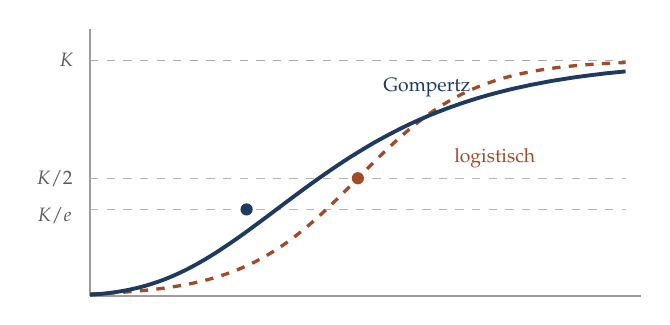
\begin{tikzpicture}[scale=1.0]
\draw[grau!60, line width=0.7pt] (0,0) -- (7.0,0);
\draw[grau!60, line width=0.7pt] (0,0) -- (0,3.4);
\draw[grau!50, dashed] (0,3.0) -- (6.8,3.0);
\node[font=\scriptsize, color=grau] at (-0.3,3.0) {$K$};
\draw[grau!45, dashed] (0,1.5) -- (6.8,1.5);
\draw[grau!45, dashed] (0,1.104) -- (6.8,1.104);
\node[font=\scriptsize, color=grau] at (-0.45,1.5) {$K/2$};
\node[font=\scriptsize, color=grau] at (-0.45,1.02) {$K/e$};
\draw[akzent, line width=1.2pt, dashed, smooth, samples=80, domain=0:6.8]
  plot (\x, {3.0/(1+exp(-1.35*(\x-3.4)))});
\draw[tief, line width=1.4pt, smooth, samples=80, domain=0:6.8]
  plot (\x, {3.0*exp(-5.0*exp(-0.68*\x))});
\fill[tief] (1.987,1.104) circle (2.2pt);
\fill[akzent] (3.4,1.5) circle (2.2pt);
\node[font=\scriptsize, color=tief, anchor=west] at (3.6,2.65) {Gompertz};
\node[font=\scriptsize, color=akzent, anchor=west] at (4.5,1.75) {logistisch};
\end{tikzpicture}
\end{center}
\end{merksatz}

\section{Ein Tumor, durchgerechnet}

\begin{merksatz}
\boxtitel{Die Größenordnungen}
\begin{center}
{\small
\renewcommand{\arraystretch}{1.48}
\begin{tabular}{@{}P{2.4cm}P{2.2cm}P{3.4cm}@{}}
\toprule
\textbf{Zellzahl} & \textbf{Masse} & \textbf{Bedeutung}\\
\midrule
$1$ & --- & erste entartete Zelle\\
$10^{6}$ & $1$ mg & Zellhaufen, ohne Gefäße\\
$10^{9}$ & $1$ g & \textcolor{akzent}{Nachweisgrenze, etwa $1$ cm}\\
$10^{12}$ & $1$ kg & meist tödliche Last\\
\bottomrule
\end{tabular}}
\end{center}

\kursiv{Faustregel:} etwa $10^{9}$ Zellen je Gramm.

\schritt{Die Parameter}
Wir setzen $K = 10^{12}$ und wählen $r$ so, dass die Verdopplungszeit bei Nachweisgröße etwa $100$ Tage beträgt --- ein für viele solide Tumoren typischer Wert.

\[ T_2 = \frac{\ln 2}{r\,\ln(K/N)} \quad\Longrightarrow\quad r = \frac{\ln 2}{T_2\,\ln(K/N)} = \frac{0{,}6931}{100 \cdot 6{,}908} = 0{,}001\ \mathrm{d}^{-1} \]
\end{merksatz}

\begin{merksatz}
\boxtitel{Der Verlauf}
\begin{center}
{\small
\renewcommand{\arraystretch}{1.46}
\begin{tabular}{@{}P{1.8cm}P{1.8cm}P{2.2cm}P{2.4cm}@{}}
\toprule
$N$ & $\ln(K/N)$ & $T_2$ & \textbf{Zeit ab 1 Zelle}\\
\midrule
$1$ & $27{,}63$ & $25$ d & $0$\\
$10^{3}$ & $20{,}72$ & $33$ d & $0{,}79$ Jahre\\
$10^{6}$ & $13{,}82$ & $50$ d & $1{,}90$ Jahre\\
$\mathbf{10^{9}}$ & $6{,}91$ & $100$ d & $\mathbf{3{,}80}$ Jahre\\
$10^{10}$ & $4{,}61$ & $151$ d & $4{,}91$ Jahre\\
$10^{11}$ & $2{,}30$ & $301$ d & $6{,}81$ Jahre\\
$K/e$ & $1{,}00$ & $693$ d & $9{,}09$ Jahre\\
$5\cdot10^{11}$ & $0{,}69$ & $1000$ d & $10{,}10$ Jahre\\
\bottomrule
\end{tabular}}
\end{center}

\kursiv{Rechnung für die letzte Spalte:} Aus $\ln(K/N) = \ln(K/N_0)\,e^{-rt}$ folgt
\[ t = -\frac{1}{r}\,\ln\frac{\ln(K/N)}{\ln(K/N_0)} = -1000\cdot\ln\frac{6{,}908}{27{,}631} = -1000\cdot\ln 0{,}25 = 1386\ \mathrm{d} . \]
\end{merksatz}

\begin{warnung}
\boxtitelr{Die verborgene Vorgeschichte}
\begin{center}
\begin{minipage}{0.9\textwidth}
\textbf{Vom Beginn bis zur Nachweisgrenze vergehen etwa vier Jahre. Vom Nachweis bis zur tödlichen Last weitere sechs.}
\end{minipage}
\end{center}

\begin{center}
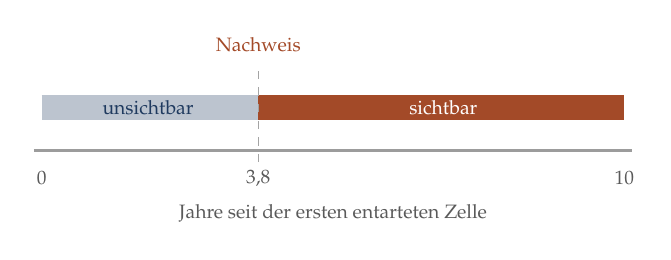
\begin{tikzpicture}[scale=1.0]
\draw[grau!60, line width=0.8pt] (0,0) -- (7.6,0);
\draw[tief!30, line width=9pt] (0.1,0.55) -- (2.85,0.55);
\draw[akzent, line width=9pt] (2.85,0.55) -- (7.5,0.55);
\node[font=\scriptsize, color=tief] at (1.45,0.55) {unsichtbar};
\node[font=\scriptsize, color=white] at (5.2,0.55) {sichtbar};
\foreach \x/\lab in {0.1/0, 2.85/{3{,}8}, 7.5/{10}}
  \node[font=\scriptsize, color=grau] at (\x,-0.35) {\lab};
\node[font=\scriptsize, color=grau] at (3.8,-0.8) {Jahre seit der ersten entarteten Zelle};
\draw[grau!55, dashed] (2.85,-0.15) -- (2.85,1.1);
\node[font=\scriptsize, color=akzent] at (2.85,1.35) {Nachweis};
\end{tikzpicture}
\end{center}

\schritt{Drei Folgerungen}
\begin{center}
{\small
\renewcommand{\arraystretch}{1.5}
\begin{tabular}{@{}P{2.8cm}P{5.8cm}@{}}
\toprule
\textbf{Streuung} & Zum Zeitpunkt der Entdeckung ist der Tumor Jahre alt. Absiedlungen können längst erfolgt sein.\\
\textbf{Ursachensuche} & Was einen Tumor ausgelöst hat, liegt Jahre vor der Diagnose. Befragungen zum letzten Jahr treffen die falsche Zeit.\\
\textbf{Früh\-erkennung} & Sie verlegt den Nachweis nach links --- mit der Vorlaufzeitverzerrung aus Band 17, Kapitel~12.\\
\bottomrule
\end{tabular}}
\end{center}

\begin{center}
\begin{minipage}{0.88\textwidth}
\kursiv{Die zweite Zeile ist ein methodisches Argument, das leicht übersehen wird: Eine Fall-Kontroll-Studie zu Tumorursachen muss nach Belastungen fragen, die zehn oder mehr Jahre zurückliegen --- und Erinnerung über solche Zeiträume ist unzuverlässig. Das ist eine Messverzerrung, die aus der Wachstumskinetik folgt.}
\end{minipage}
\end{center}
\end{warnung}

\begin{warnung}
\boxtitelr{Und die Deutung von Verlaufskontrollen}
Wächst ein bekannter Tumor langsamer als vorher, so kann das dreierlei bedeuten:

\begin{center}
\renewcommand{\arraystretch}{1.5}
\begin{tabular}{@{}P{2.4cm}P{6.2cm}@{}}
\toprule
\textbf{Therapie wirkt} & $r$ ist gesunken.\\
\textbf{Nichts} & Gompertz-Wachstum verlangsamt sich \kursiv{von selbst}.\\
\textbf{Beides} & Die häufigste Lage.\\
\bottomrule
\end{tabular}
\end{center}

\begin{center}
\begin{minipage}{0.9\textwidth}
\textbf{Ohne Vergleichsgruppe lässt sich das nicht trennen.} Die natürliche Verlangsamung sieht aus wie ein Behandlungserfolg.
\end{minipage}
\end{center}

\begin{center}
\begin{minipage}{0.88\textwidth}
\kursiv{Das ist derselbe Sachverhalt wie die Regression zur Mitte in Band 17, Kapitel~10: Ein Verlauf, der ohnehin eingetreten wäre, wird der Maßnahme zugeschrieben. Und die Abhilfe ist dieselbe --- Randomisierung.}
\end{minipage}
\end{center}
\end{warnung}

\section{Die Wirkung einer Behandlung}

\begin{merksatz}
\boxtitel{Die Annahme vom festen Anteil}
\begin{center}
\begin{minipage}{0.9\textwidth}
\textbf{Eine gegebene Dosis tötet stets denselben \kursiv{Anteil} der vorhandenen Zellen --- nicht dieselbe Zahl.}
\end{minipage}
\end{center}

Man nennt das die \Begriff{Log-kill-Annahme}. Eine Behandlung, die $99{,}9\,\%$ tötet, senkt die Zellzahl um drei Zehnerpotenzen --- gleichgültig, ob $10^{12}$ oder $10^{6}$ Zellen vorhanden waren.

\schritt{Warum das plausibel ist}
Jede Zelle wird unabhängig von den anderen mit derselben Wahrscheinlichkeit getroffen. Das ist dieselbe Annahme wie beim Zerfall in Kapitel~1 --- nur auf die Dosis statt auf die Zeit bezogen.

\schritt{Die unbequeme Folgerung}
\begin{center}
{\small
\renewcommand{\arraystretch}{1.48}
\begin{tabular}{@{}P{2.4cm}P{2.4cm}P{2.8cm}@{}}
\toprule
\textbf{vorher} & \textbf{nachher} & \textbf{getötet}\\
\midrule
$10^{12}$ & $10^{9}$ & $999$ Milliarden\\
$10^{9}$ & $10^{6}$ & $999$ Millionen\\
$10^{3}$ & $1$ & $999$\\
\bottomrule
\end{tabular}}
\end{center}

\begin{center}
\begin{minipage}{0.9\textwidth}
\textbf{Um von $10^{12}$ auf null zu kommen, braucht man nicht eine, sondern viele gleich wirksame Gaben.} Und die letzte Zelle ist genauso schwer zu treffen wie die erste Milliarde.
\end{minipage}
\end{center}

\begin{center}
\begin{minipage}{0.88\textwidth}
\kursiv{Das erklärt, warum Chemotherapien in Zyklen gegeben werden und warum ein vollständiges Verschwinden im Bild --- unter $10^{9}$ Zellen --- keine Heilung bedeutet. Zwischen \enquote{nicht nachweisbar} und \enquote{nicht vorhanden} liegen bis zu neun Zehnerpotenzen.}
\end{minipage}
\end{center}
\end{merksatz}

\begin{merksatz}
\boxtitel{Sechs Zyklen, durchgerechnet}
Ausgangslast $10^{12}$, je Zyklus drei Zehnerpotenzen, $21$ Tage Abstand.

\begin{center}
{\small
\renewcommand{\arraystretch}{1.46}
\begin{tabular}{@{}P{1.6cm}P{2.2cm}P{2.4cm}P{1.8cm}@{}}
\toprule
\textbf{Zyklus} & \textbf{nach Gabe} & \textbf{nach 21 d} & \textbf{Faktor}\\
\midrule
$1$ & $1{,}0\cdot10^{9}$ & $1{,}15\cdot10^{9}$ & $1{,}15$\\
$2$ & $1{,}15\cdot10^{6}$ & $1{,}53\cdot10^{6}$ & $1{,}33$\\
$3$ & $1{,}53\cdot10^{3}$ & $2{,}34\cdot10^{3}$ & $1{,}52$\\
$4$ & $2{,}34$ & $4{,}08$ & $1{,}74$\\
$5$ & $0{,}0041$ & $0{,}0081$ & $1{,}99$\\
$6$ & $8\cdot10^{-6}$ & --- & \textcolor{gruen}{Heilung}\\
\bottomrule
\end{tabular}}
\end{center}

\schritt{Die Beobachtung}
Der Wiederanwuchs zwischen den Zyklen wird von Zyklus zu Zyklus \kursiv{stärker} --- von Faktor $1{,}15$ auf $1{,}99$.

\begin{center}
\begin{minipage}{0.88\textwidth}
\kursiv{Der Grund steht in Definition 13.1: Je kleiner $N$, desto größer $\ln(K/N)$ und damit die Wachstumsrate je Zelle. Ein kleiner Resttumor wächst schneller nach als ein großer. Das ist die \Begriff{Norton-Simon-Hypothese} --- und aus ihr folgt die Empfehlung, die Abstände zwischen den Zyklen so kurz wie vertretbar zu halten.}
\end{minipage}
\end{center}

\schritt{Das Modell sagt Heilung vorher}
Nach sechs Zyklen liegt die berechnete Zellzahl weit unter eins. Nach diesem Modell wäre jeder Tumor heilbar.

\begin{center}
\begin{minipage}{0.9\textwidth}
\textbf{Er ist es nicht.} Der Grund fehlt in diesem Modell vollständig --- und ist der Gegenstand des nächsten Kapitels.
\end{minipage}
\end{center}
\end{merksatz}

\section{Der Bruchfall}

\begin{warnung}
\boxtitelr{Vier Lücken}
\begin{center}
{\small
\renewcommand{\arraystretch}{1.5}
\begin{tabular}{@{}P{2.4cm}P{6.2cm}@{}}
\toprule
\textbf{Keine Resistenz} & Alle Zellen sind gleich empfindlich. Kapitel~14.\\
\textbf{Keine ganzen Zahlen} & Bei $N = 0{,}0041$ rechnet das Modell weiter. Unterhalb weniger Zellen braucht man ein zufallsgestütztes Modell.\\
\textbf{$r$ fest} & Tumoren verändern sich; die Wachstumsrate ist keine Konstante.\\
\textbf{Unendliche Rate} & Bei $N \to 0$ geht $\ln(K/N) \to \infty$.\\
\bottomrule
\end{tabular}}
\end{center}

\schritt{Zur letzten Zeile}
Das Modell behauptet, eine einzelne übrig gebliebene Zelle teile sich alle $25$ Tage --- was noch plausibel ist. Bei $N = 10^{-6}$ wären es rechnerisch alle $17$ Tage, und das ist sinnlos.

\begin{center}
\begin{minipage}{0.88\textwidth}
\kursiv{Praktisch stört das wenig, weil der Bereich unter einer Zelle ohnehin außerhalb der Modellgültigkeit liegt. Man sollte aber wissen, dass die Zahlen dort nichts mehr bedeuten --- und insbesondere, dass \enquote{$N = 10^{-6}$} keine Aussage über Heilungswahrscheinlichkeit ist.}
\end{minipage}
\end{center}

\schritt{Was man stattdessen sagen kann}
Ist die berechnete mittlere Zellzahl $\mu$ sehr klein, so beträgt die Wahrscheinlichkeit, dass keine Zelle überlebt, näherungsweise
\[ \Pr[\text{Heilung}] = e^{-\mu} . \]

\begin{center}
\renewcommand{\arraystretch}{1.45}
\begin{tabular}{@{}P{2.0cm}P{2.6cm}P{2.4cm}@{}}
\toprule
$\mu$ & $e^{-\mu}$ & \\
\midrule
$5$ & $0{,}7\,\%$ & \\
$1$ & $36{,}8\,\%$ & \\
$0{,}1$ & $90{,}5\,\%$ & \\
$0{,}01$ & $99{,}0\,\%$ & \\
\bottomrule
\end{tabular}
\end{center}

\begin{center}
\begin{minipage}{0.88\textwidth}
\kursiv{Das ist die Poisson-Näherung --- und sie macht aus einer sinnlosen Zahl eine sinnvolle. Sie ist zugleich die Grundlage der Modelle zur Bestrahlungsplanung, wo die Heilungswahrscheinlichkeit genau so berechnet wird.}
\end{minipage}
\end{center}
\end{warnung}

\section{Übungsaufgaben}

\begin{aufgabe}
\boxtitel{Aufgabe 13.1 --- Die Vorgeschichte berechnen}
Ein Tumor wird mit $2$ cm Durchmesser entdeckt. Bei der Voruntersuchung zwölf Monate zuvor war nichts zu sehen. Die Verdopplungszeit bei dieser Größe beträgt $120$ Tage, $K = 10^{12}$. War der Tumor vor einem Jahr schon da?

\loesung
\schritt{Schritt 1 --- Die Zellzahl bestimmen}
Eine Kugel von $2$ cm Durchmesser hat das Volumen
\[ V = \frac{4}{3}\pi\left(1\ \mathrm{cm}\right)^{3} = 4{,}19\ \mathrm{cm^3} \approx 4{,}2\ \mathrm{g} \]
Mit $10^{9}$ Zellen je Gramm:
\[ N = 4{,}2\cdot10^{9} \]

\schritt{Schritt 2 --- Die Wachstumskonstante}
\[ \ln\frac{K}{N} = \ln\frac{10^{12}}{4{,}2\cdot10^{9}} = \ln 238{,}1 = 5{,}473 \]
\[ r = \frac{\ln 2}{T_2 \cdot \ln(K/N)} = \frac{0{,}6931}{120 \cdot 5{,}473} = 0{,}001055\ \mathrm{d}^{-1} \]

\schritt{Schritt 3 --- Rückwärts rechnen}
Aus $\ln(K/N_t) = \ln(K/N_0)e^{-rt}$ folgt rückwärts, also mit $t = -365$:
\[ \ln\frac{K}{N_{\text{vorher}}} = 5{,}473 \cdot e^{+0{,}001055 \cdot 365} = 5{,}473 \cdot e^{0{,}3851} = 5{,}473 \cdot 1{,}4698 = 8{,}044 \]

\schritt{Schritt 4 --- Die Zellzahl}
\[ \frac{K}{N} = e^{8{,}044} = 3117 \quad\Longrightarrow\quad N = \frac{10^{12}}{3117} = 3{,}21\cdot10^{8} \]

\schritt{Schritt 5 --- Die Größe}
\[ 3{,}21\cdot10^{8}\ \text{Zellen} = 0{,}32\ \mathrm{g} = 0{,}32\ \mathrm{cm^3} \]
\[ r = \sqrt[3]{\frac{3 \cdot 0{,}32}{4\pi}} = \sqrt[3]{0{,}0764} = 0{,}424\ \mathrm{cm} \]
Durchmesser: $0{,}85$ cm.

\schritt{Antwort}
\begin{center}
\begin{minipage}{0.9\textwidth}
\textbf{Ja --- der Tumor war vor einem Jahr bereits knapp $9$ mm groß.}
\end{minipage}
\end{center}

\schritt{Schritt 6 --- Die Folgerung}
Ein Knoten von $9$ mm liegt an der Nachweisgrenze vieler Verfahren, aber nicht darunter. Dass er nicht gesehen wurde, bedeutet nicht, dass er nicht da war.

\begin{center}
\begin{minipage}{0.88\textwidth}
\kursiv{Das ist ein Befund, der in der Begutachtung eine Rolle spielt: Ob ein Tumor bei einer früheren Untersuchung hätte erkannt werden müssen, lässt sich mit dieser Rechnung eingrenzen. Sie liefert eine Größenabschätzung, keine Gewissheit --- die Verdopplungszeit streut zwischen Tumoren erheblich.}
\end{minipage}
\end{center}

\schritt{Schritt 7 --- Und die Empfindlichkeit prüfen}
Bei $T_2 = 60$ Tagen statt $120$:
\[ r = 0{,}002110, \qquad \ln\frac{K}{N} = 5{,}473\,e^{0{,}7702} = 11{,}82 \]
\[ N = 10^{12}\,e^{-11{,}82} = 7{,}3\cdot10^{6} \ \text{Zellen} = 7{,}3\ \mathrm{mg} \]
Durchmesser: etwa $2{,}4$ mm --- unter jeder Nachweisgrenze.

\begin{center}
\begin{minipage}{0.86\textwidth}
\kursiv{Halbierte Verdopplungszeit, und die Antwort kehrt sich um. Die Rechnung ist so gut wie die Schätzung der Verdopplungszeit --- und die ist meist nicht bekannt.}
\end{minipage}
\end{center}
\end{aufgabe}

\begin{aufgabe}
\boxtitel{Aufgabe 13.2 --- Zyklusabstände vergleichen}
Ein Schema tötet je Gabe $99\,\%$ der Zellen. Vergleichen Sie Abstände von $14$, $21$ und $28$ Tagen bei einer Ausgangslast von $10^{11}$ und $r = 0{,}001$, $K = 10^{12}$. Wie viele Zyklen bis unter eine Zelle?

\loesung
\schritt{Schritt 1 --- Die Rechenschritte}
Je Zyklus: Zellzahl durch $100$ teilen, dann $\tau$ Tage Gompertz-Wachstum:
\[ \ln\frac{K}{N_{\text{neu}}} = \ln\frac{K}{N}\cdot e^{-r\tau} \]

\schritt{Schritt 2 --- Die Wachstumsfaktoren}
\begin{center}
\renewcommand{\arraystretch}{1.45}
\begin{tabular}{@{}P{1.8cm}P{2.2cm}P{2.8cm}@{}}
\toprule
$\tau$ & $e^{-r\tau}$ & \\
\midrule
$14$ d & $0{,}9861$ & \\
$21$ d & $0{,}9792$ & \\
$28$ d & $0{,}9724$ & \\
\bottomrule
\end{tabular}
\end{center}

\schritt{Schritt 3 --- Der Verlauf bei $\tau = 21$ Tagen}
Start: $N = 10^{11}$, also $\ln(K/N) = 2{,}303$.

\begin{center}
{\small
\renewcommand{\arraystretch}{1.44}
\begin{tabular}{@{}P{1.4cm}P{2.2cm}P{2.2cm}P{2.2cm}@{}}
\toprule
\textbf{Zykl.} & \textbf{nach Gabe} & $\ln(K/N)$ & \textbf{nach $21$ d}\\
\midrule
$1$ & $1{,}0\cdot10^{9}$ & $6{,}908$ & $1{,}16\cdot10^{9}$\\
$2$ & $1{,}16\cdot10^{7}$ & $11{,}36$ & $1{,}45\cdot10^{7}$\\
$3$ & $1{,}45\cdot10^{5}$ & $15{,}75$ & $1{,}94\cdot10^{5}$\\
$4$ & $1{,}94\cdot10^{3}$ & $20{,}06$ & $2{,}77\cdot10^{3}$\\
$5$ & $27{,}7$ & $24{,}31$ & $42{,}2$\\
$6$ & $0{,}422$ & $28{,}49$ & $0{,}68$\\
\bottomrule
\end{tabular}}
\end{center}

Nach dem \textbf{sechsten Zyklus} liegt die Zellzahl unter eins.

\schritt{Schritt 4 --- Der Vergleich der Abstände}
\begin{center}
{\small
\renewcommand{\arraystretch}{1.48}
\begin{tabular}{@{}P{1.8cm}P{2.2cm}P{2.2cm}P{2.0cm}@{}}
\toprule
$\tau$ & \textbf{Zyklen} & \textbf{Gesamtdauer} & \textbf{Rest nach 6}\\
\midrule
$14$ d & $6$ & $84$ d & $0{,}30$\\
$21$ d & $6$ & $126$ d & $0{,}68$\\
$28$ d & $7$ & $196$ d & $1{,}56$\\
\bottomrule
\end{tabular}}
\end{center}

\schritt{Schritt 5 --- Die Deutung}
\begin{center}
\begin{minipage}{0.9\textwidth}
\textbf{Der Unterschied ist gering, aber gerichtet: Kürzere Abstände lassen weniger Restzellen übrig.}
\end{minipage}
\end{center}

Mit der Poisson-Näherung aus Abschnitt 13.5:
\begin{center}
\renewcommand{\arraystretch}{1.45}
\begin{tabular}{@{}P{1.8cm}P{2.2cm}P{2.8cm}@{}}
\toprule
$\tau$ & $\mu$ & $\Pr[\text{Heilung}]$\\
\midrule
$14$ d & $0{,}30$ & $74{,}1\,\%$\\
$21$ d & $0{,}68$ & $50{,}7\,\%$\\
$28$ d & $1{,}56$ & $21{,}0\,\%$\\
\bottomrule
\end{tabular}
\end{center}

\begin{center}
\begin{minipage}{0.88\textwidth}
\kursiv{Aus einem scheinbar kleinen Unterschied in der Restzellzahl wird ein großer in der Heilungswahrscheinlichkeit --- weil die Exponentialfunktion dazwischensteht. Das ist der rechnerische Kern der \Begriff{dosisdichten Therapie}: dieselben Gaben, kürzere Abstände. Studien haben für mehrere Tumorarten einen Vorteil gezeigt.}
\end{minipage}
\end{center}

\schritt{Schritt 6 --- Der Vorbehalt}
Kürzere Abstände bedeuten weniger Erholungszeit für gesundes Gewebe. Der Nutzen ist erkauft, und ob er überwiegt, entscheidet die Studie, nicht das Modell.
\end{aufgabe}

\begin{aufgabe}
\boxtitel{Aufgabe 13.3 --- Gompertz und Logistik vergleichen}
Zeigen Sie, dass sich beide Modelle bei kleinem $N$ ähnlich verhalten, und beziffern Sie, wann sie sich trennen.

\loesung
\schritt{Schritt 1 --- Die Wachstumsraten je Zelle}
\[ \text{logistisch: } \frac{1}{N}\frac{\dd N}{\dd t} = r_L\left(1-\frac{N}{K}\right) \]
\[ \text{Gompertz: } \frac{1}{N}\frac{\dd N}{\dd t} = r_G\,\ln\frac{K}{N} \]

\schritt{Schritt 2 --- Auf denselben Ausgangswert bringen}
Bei sehr kleinem $N$ ist die logistische Rate $\approx r_L$. Die Gompertz-Rate hängt von $N$ ab; wir passen bei $N_0 = 10^{6}$ an:
\[ r_L = r_G\,\ln\frac{K}{N_0} = 0{,}001 \cdot 13{,}816 = 0{,}01382\ \mathrm{d}^{-1} \]

\schritt{Schritt 3 --- Der Vergleich}
\begin{center}
{\small
\renewcommand{\arraystretch}{1.46}
\begin{tabular}{@{}P{1.8cm}P{2.2cm}P{2.2cm}P{1.8cm}@{}}
\toprule
$N$ & \textbf{logistisch} & \textbf{Gompertz} & \textbf{Verhältnis}\\
\midrule
$10^{6}$ & $0{,}01382$ & $0{,}01382$ & $1{,}00$\\
$10^{8}$ & $0{,}01382$ & $0{,}00921$ & $0{,}67$\\
$10^{9}$ & $0{,}01381$ & $0{,}00691$ & $0{,}50$\\
$10^{10}$ & $0{,}01368$ & $0{,}00461$ & $0{,}34$\\
$10^{11}$ & $0{,}01244$ & $0{,}00230$ & $0{,}19$\\
$5\cdot10^{11}$ & $0{,}00691$ & $0{,}00069$ & $0{,}10$\\
\bottomrule
\end{tabular}}
\end{center}

\kursiv{Rechnung für $N=10^{10}$:} logistisch $0{,}01382(1-0{,}01) = 0{,}01368$; Gompertz $0{,}001\cdot\ln(100) = 0{,}004605$.

\schritt{Schritt 4 --- Die Deutung}
\begin{center}
\begin{minipage}{0.9\textwidth}
\textbf{Das logistische Modell bremst praktisch gar nicht, solange $N \ll K$.} Erst bei einem Prozent der Endgröße hat es $1\,\%$ verloren. Gompertz hat dort bereits zwei Drittel der Rate eingebüßt.
\end{minipage}
\end{center}

\schritt{Schritt 5 --- Wo sie sich um die Hälfte unterscheiden}
Gesucht ist $N$ mit
\[ r_G\ln\frac{K}{N} = \frac12\,r_L = \frac12\,r_G\ln\frac{K}{N_0} \]
\[ \ln\frac{K}{N} = \frac{13{,}816}{2} = 6{,}908 \quad\Longrightarrow\quad \frac{K}{N} = 10^{3} \quad\Longrightarrow\quad N = 10^{9} \]

\textbf{Genau an der Nachweisgrenze} --- was die Tabelle bestätigt.

\schritt{Schritt 6 --- Warum das die Modellwahl entscheidet}
\begin{center}
\begin{minipage}{0.88\textwidth}
\kursiv{Im Bereich, den man \kursiv{sieht} --- von $10^{9}$ bis $10^{12}$ ---, unterscheiden sich die Modelle erheblich. Genau dort werden die Daten erhoben, und genau dort passt Gompertz besser. Im unsichtbaren Bereich sind sie kaum zu unterscheiden, und dort wäre es auch gleichgültig.}
\end{minipage}
\end{center}

\begin{center}
\begin{minipage}{0.88\textwidth}
\kursiv{Das ist eine allgemeine Einsicht zur Modellwahl: Zwei Modelle unterscheiden zu können verlangt, dass man in dem Bereich misst, wo sie auseinandergehen. Bei Tumoren ist das glücklicherweise der beobachtbare --- bei der Epidemieendgröße in Kapitel~7 war es umgekehrt.}
\end{minipage}
\end{center}
\end{aufgabe}

\begin{geschichte}
\boxtitelg{Eine Sterbetafel und ein Tumor}
\Person{Benjamin Gompertz} (1779--1865) war Versicherungsmathematiker in London --- und als Jude von der Universität ausgeschlossen; er bildete sich selbst aus.

1825 veröffentlichte er eine Arbeit über Sterbetafeln mit einer einfachen Behauptung: \textbf{Die Sterberate wächst mit dem Alter exponentiell.}

\begin{center}
\begin{minipage}{0.9\textwidth}
\kursiv{Das Gompertz-Gesetz gilt bis heute erstaunlich gut --- zwischen etwa dreißig und neunzig Jahren verdoppelt sich die Sterbewahrscheinlichkeit etwa alle acht Jahre, in allen untersuchten Bevölkerungen und über zwei Jahrhunderte hinweg. Es ist eine der beständigsten empirischen Regelmäßigkeiten der Biologie.}
\end{minipage}
\end{center}

\schritt{Der Weg zum Tumorwachstum}
Die Verbindung ist rein formal: Gompertz' Sterbetafel und die Wachstumskurve dieses Kapitels führen auf dieselbe Funktion, weil in beiden Fällen eine Größe exponentiell mit der Zeit abnimmt --- dort die Überlebenswahrscheinlichkeit, hier $\ln(K/N)$.

\Person{Anna Kane Laird} zeigte 1964, dass die Funktion Tumorwachstumsdaten außergewöhnlich gut beschreibt --- besser als jedes andere damals geprüfte Modell.

\begin{center}
\begin{minipage}{0.9\textwidth}
\kursiv{Laird prüfte Daten von neunzehn Tumorarten in Maus, Ratte und Kaninchen und fand die Gompertz-Form durchweg bestätigt. Bemerkenswert ist, dass sie keine Begründung dafür angeben konnte --- und es bis heute keine allgemein anerkannte gibt. Das Modell ist gut, weil es passt, nicht weil man wüsste, warum.}
\end{minipage}
\end{center}

\schritt{Die Log-kill-Annahme}
\Person{Howard Skipper} formulierte sie in den 1960er Jahren aufgrund von Versuchen an einer Mäuseleukämie. Sein Befund war damals überraschend und bestimmt bis heute, wie Chemotherapieschemata entworfen werden.

\begin{center}
\begin{minipage}{0.9\textwidth}
\kursiv{Skipper zeigte zugleich, dass die Heilung nur gelingt, wenn die \kursiv{letzte} Zelle getötet wird --- daher der Grundsatz, die Behandlung über das sichtbare Verschwinden hinaus fortzusetzen. Das war eine Umkehr der bisherigen Praxis.}
\end{minipage}
\end{center}
\end{geschichte}

\begin{forschung}
\boxtitelp{Tumormodellierung heute}
\begin{center}
{\small
\renewcommand{\arraystretch}{1.45}
\begin{tabular}{@{}P{2.8cm}P{5.4cm}@{}}
\toprule
\textbf{Modell\-vergleiche} & Systematische Prüfungen an Tierdaten finden regelmäßig, dass einfache Modelle mit wenigen Parametern besser vorhersagen als komplizierte.\\
\textbf{Räumliche Modelle} & Tumoren als wachsende Gewebe mit Sauerstoffgefälle und Gefäßversorgung.\\
\textbf{Vorhersage am Einzelfall} & Aus zwei bis drei Bildkontrollen das weitere Wachstum schätzen.\\
\bottomrule
\end{tabular}}
\end{center}

\schritt{Zur ersten Zeile}
Vergleiche zwischen exponentiellem, logistischem, Gompertz- und Potenzgesetzmodell an großen Datensammlungen zeigen: Die Gompertz-Form beschreibt vorhandene Daten am besten, das einfachere Potenzgesetz sagt künftiges Wachstum oft besser vorher.

\begin{center}
\begin{minipage}{0.88\textwidth}
\kursiv{Das ist derselbe Sachverhalt wie bei Pearls Bevölkerungsvorhersage in Kapitel~2: Gute Anpassung und gute Vorhersage sind zweierlei. Ein Modell mit einer Kapazitätsgrenze schätzt diese Grenze aus Daten, die weit davon entfernt liegen --- und die Schätzung ist entsprechend unzuverlässig.}
\end{minipage}
\end{center}

\schritt{Zur dritten Zeile}
Der praktisch interessanteste Ansatz: Aus wenigen Verlaufskontrollen die Parameter schätzen und den weiteren Verlauf --- mit und ohne Behandlung --- vorhersagen.

\begin{center}
\begin{minipage}{0.88\textwidth}
\kursiv{Die Schwierigkeit ist dieselbe wie in Kapitel~2: Zwei Messpunkte bestimmen zwei Parameter, aber ohne jede Sicherheit. Man braucht Bevölkerungsmodelle wie in Kapitel~10 --- die Verteilung der Parameter über viele Patienten als Vorwissen, verfeinert durch die Messungen am einzelnen.}
\end{minipage}
\end{center}
\end{forschung}

\begin{merksatz}
\boxtitel{Was Sie jetzt können}
\begin{center}
\renewcommand{\arraystretch}{1.5}
\begin{tabular}{@{}P{3.0cm}P{5.6cm}@{}}
\toprule
\textbf{Definition 13.1} & logarithmische statt linearer Bremsung\\
\textbf{Satz 13.2} & Lösung über die Substitution $u = \ln(K/N)$\\
\textbf{Satz 13.3} & Wendepunkt bei $K/e$, nicht $K/2$\\
\textbf{Log-kill} & fester Anteil, nicht feste Zahl\\
\textbf{Poisson} & $\Pr[\text{Heilung}] = e^{-\mu}$\\
\bottomrule
\end{tabular}
\end{center}

\begin{center}
\begin{minipage}{0.88\textwidth}
\kursiv{Dieses Kapitel sagte Heilung vorher, wo es keine gibt. Im nächsten fügen wir das ein, was fehlte --- und finden dabei ein Behandlungsprinzip, das dem gewohnten widerspricht.}
\end{minipage}
\end{center}
\end{merksatz}

\chapter{Resistenz und Evolution}

\section{Was fehlte}

\begin{merksatz}
\boxtitel{Der Widerspruch aus Kapitel 13}
Das Log-kill-Modell sagte vollständige Heilung vorher. Tatsächlich kehren viele Tumoren wieder, und viele Infektionen sprechen nach einiger Zeit nicht mehr an.

\begin{center}
\begin{minipage}{0.9\textwidth}
\textbf{Der fehlende Baustein: Nicht alle Zellen sind gleich empfindlich.} Ein kleiner Teil überlebt jede Gabe --- und genau dieser Teil vermehrt sich danach.
\end{minipage}
\end{center}

\schritt{Die Frage, die dahintersteht}
\begin{center}
\renewcommand{\arraystretch}{1.5}
\begin{tabular}{@{}P{2.4cm}P{6.2cm}@{}}
\toprule
\textbf{Erworben} & Die Behandlung \kursiv{macht} Zellen unempfindlich.\\
\textbf{Vorbestehend} & Unempfindliche Zellen waren schon da; die Behandlung \kursiv{wählt} sie aus.\\
\bottomrule
\end{tabular}
\end{center}

\begin{center}
\begin{minipage}{0.88\textwidth}
\kursiv{Die Frage klingt akademisch und ist es nicht: Beide Fälle verlangen völlig verschiedene Behandlungsstrategien. Abschnitt 14.3 zeigt, wie man sie unterscheidet --- mit einem Versuch, der ohne jede molekulare Untersuchung auskommt.}
\end{minipage}
\end{center}
\end{merksatz}

\section{Wann Resistenz entsteht}

\begin{merksatz}
\boxtitel{Satz 14.1 --- die Goldie-Coldman-Abschätzung}
Entstehen unempfindliche Zellen bei jeder Teilung mit der Wahrscheinlichkeit $\mu$, so beträgt bei einer Zellzahl $N$ die Wahrscheinlichkeit, dass \kursiv{keine} vorhanden ist, näherungsweise
\[ \Pr[\text{keine Resistenz}] \approx e^{-\mu N} . \]

\schritt{Begründung}
Um von einer Zelle auf $N$ zu kommen, sind etwa $N$ Teilungen nötig --- jede Zelle außer der ersten entstand durch eine.

Die erwartete Zahl unempfindlicher Zellen ist also etwa $\mu N$. Sind die Ereignisse selten und unabhängig, so folgt ihre Zahl näherungsweise einer Poisson-Verteilung, und die Wahrscheinlichkeit für null Ereignisse ist $e^{-\mu N}$. $\blacksquare$

\begin{center}
\begin{minipage}{0.88\textwidth}
\kursiv{Es ist dieselbe Poisson-Näherung wie am Ende von Kapitel~13 --- nur diesmal für das Auftreten statt für das Überleben.}
\end{minipage}
\end{center}
\end{merksatz}

\begin{warnung}
\boxtitelr{Die Zahlen sind unbequem}
Mit $\mu = 10^{-6}$ je Teilung:

\begin{center}
{\small
\renewcommand{\arraystretch}{1.48}
\begin{tabular}{@{}P{1.8cm}P{2.4cm}P{2.8cm}@{}}
\toprule
$N$ & $\mu N$ & $\Pr[\text{keine}]$\\
\midrule
$10^{3}$ & $0{,}001$ & $99{,}9\,\%$\\
$10^{4}$ & $0{,}01$ & $99{,}0\,\%$\\
$10^{5}$ & $0{,}1$ & $90{,}5\,\%$\\
$\mathbf{10^{6}}$ & $\mathbf{1}$ & $\mathbf{36{,}8\,\%}$\\
$10^{7}$ & $10$ & $0{,}005\,\%$\\
$10^{9}$ & $1000$ & \textcolor{akzent}{praktisch null}\\
\bottomrule
\end{tabular}}
\end{center}

\schritt{Die kritische Größe}
\[ N_c = \frac{1}{\mu} = 10^{6} \ \text{Zellen} = 1\ \mathrm{mg} \]

\begin{center}
\begin{minipage}{0.9\textwidth}
\textbf{Ein Tumor von einem Milligramm enthält mit Wahrscheinlichkeit $63\,\%$ bereits unempfindliche Zellen.} Die Nachweisgrenze liegt tausendfach höher.
\end{minipage}
\end{center}

\begin{center}
\begin{minipage}{0.88\textwidth}
\kursiv{Damit ist die Lage beschrieben, in der jede Behandlung beginnt: \textbf{Zum Zeitpunkt der Diagnose sind unempfindliche Zellen mit Sicherheit vorhanden.} Nicht, weil die Behandlung sie erzeugt hätte --- sondern weil sie in einem Tumor dieser Größe zwangsläufig entstehen.}
\end{minipage}
\end{center}

\schritt{Die praktische Folgerung, die Goldie und Coldman zogen}
Je früher behandelt wird und je mehr voneinander unabhängige Mittel gleichzeitig gegeben werden, desto geringer die Wahrscheinlichkeit, dass eine Zelle gegen \kursiv{alle} unempfindlich ist.

Bei zwei unabhängigen Mitteln:
\[ \Pr[\text{gegen beide}] = \mu^2 = 10^{-12} \quad\Longrightarrow\quad N_c = 10^{12} . \]

\begin{center}
\begin{minipage}{0.88\textwidth}
\kursiv{Das ist die rechnerische Begründung der Kombinationstherapie --- in der Onkologie wie bei Tuberkulose und HIV, wo regelmäßig drei oder vier Mittel gleichzeitig gegeben werden. Die Voraussetzung ist \kursiv{Unabhängigkeit}: Die Resistenzmechanismen dürfen einander nicht bedingen. Trifft das nicht zu, bricht die Rechnung zusammen.}
\end{minipage}
\end{center}
\end{warnung}

\section{Vorher oder nachher --- der Versuch von Luria und Delbrück}

\begin{merksatz}
\boxtitel{Die Frage und der Kunstgriff}
1943 war umstritten, ob Bakterien durch den Kontakt mit einem Virus unempfindlich \kursiv{werden} oder ob unempfindliche Bakterien bereits vorhanden sind.

\begin{center}
\begin{minipage}{0.9\textwidth}
\textbf{Luria und Delbrück entschieden die Frage ohne jede Beobachtung des Vorgangs --- allein durch die \kursiv{Streuung} der Ergebnisse.}
\end{minipage}
\end{center}

\schritt{Der Versuchsaufbau}
Man lässt viele getrennte Kulturen aus wenigen Zellen anwachsen, setzt dann jede dem Virus aus und zählt die überlebenden Kolonien.
\end{merksatz}

\begin{merksatz}
\boxtitel{Satz 14.2 --- die beiden Vorhersagen}
\begin{center}
{\small
\renewcommand{\arraystretch}{1.55}
\begin{tabular}{@{}P{2.2cm}P{3.0cm}P{3.0cm}@{}}
\toprule
& \textbf{erworben} & \textbf{vorbestehend}\\
\midrule
Wann & bei Kontakt & während des Wachstums\\
Zahl je Kultur & Poisson & \textcolor{akzent}{stark gestreut}\\
$\operatorname{Var}/\text{Mittel}$ & $\approx 1$ & \textcolor{akzent}{$\gg 1$}\\
\bottomrule
\end{tabular}}
\end{center}

\schritt{Warum bei Erwerb Poisson}
Jede der $N$ Zellen wird beim Kontakt unabhängig mit derselben kleinen Wahrscheinlichkeit unempfindlich. Das ist genau die Lage, in der die Poisson-Verteilung gilt --- und für sie ist die Varianz gleich dem Mittelwert.

\schritt{Warum bei Vorbestehen nicht}
Eine Mutation, die \kursiv{früh} im Wachstum auftritt, wird mit der Kultur vervielfältigt. Aus einer einzigen frühen Mutation werden Tausende von Nachkommen.

\begin{center}
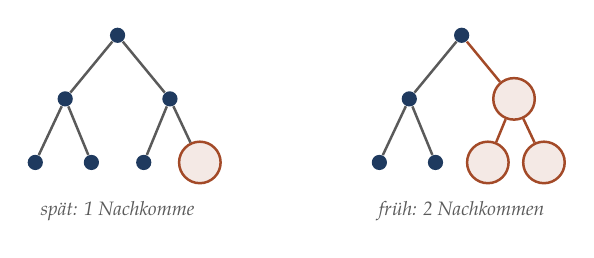
\begin{tikzpicture}[scale=0.95]
\begin{scope}
\node[knoten] (w) at (0,1.7) {};
\node[knoten] (a) at (-0.7,0.85) {}; \node[knoten] (b) at (0.7,0.85) {};
\node[knoten] (a1) at (-1.1,0) {}; \node[knoten] (a2) at (-0.35,0) {};
\node[knoten] (b1) at (0.35,0) {}; \node[knotenr] (b2) at (1.1,0) {};
\draw[kante] (w)--(a); \draw[kante] (w)--(b);
\draw[kante] (a)--(a1); \draw[kante] (a)--(a2);
\draw[kante] (b)--(b1); \draw[kante] (b)--(b2);
\node[font=\scriptsize\itshape, color=grau] at (0,-0.65) {spät: 1 Nachkomme};
\end{scope}
\begin{scope}[xshift=4.6cm]
\node[knoten] (w) at (0,1.7) {};
\node[knoten] (a) at (-0.7,0.85) {}; \node[knotenr] (b) at (0.7,0.85) {};
\node[knoten] (a1) at (-1.1,0) {}; \node[knoten] (a2) at (-0.35,0) {};
\node[knotenr] (b1) at (0.35,0) {}; \node[knotenr] (b2) at (1.1,0) {};
\draw[kante] (w)--(a); \draw[kante, akzent] (w)--(b);
\draw[kante] (a)--(a1); \draw[kante] (a)--(a2);
\draw[kante, akzent] (b)--(b1); \draw[kante, akzent] (b)--(b2);
\node[font=\scriptsize\itshape, color=grau] at (0,-0.65) {früh: 2 Nachkommen};
\end{scope}
\end{tikzpicture}
\end{center}

\begin{center}
\begin{minipage}{0.9\textwidth}
\textbf{In den meisten Kulturen trat keine frühe Mutation auf --- dort findet man wenige oder keine Überlebenden. In den wenigen mit früher Mutation findet man sehr viele.} Das erzeugt eine enorme Streuung.
\end{minipage}
\end{center}
\end{merksatz}

\begin{merksatz}
\boxtitel{Ein Zahlenbeispiel}
Zwanzig Kulturen, gezählte Kolonien:
\[ 1,\ 0,\ 3,\ 0,\ 0,\ 5,\ 0,\ 5,\ 0,\ 6,\ 107,\ 0,\ 0,\ 0,\ 1,\ 0,\ 0,\ 64,\ 0,\ 35 \]

\schritt{Mittelwert}
\[ \MW = \frac{1+3+5+5+6+107+1+64+35}{20} = \frac{227}{20} = 11{,}35 \]

\schritt{Varianz}
\[ \sum x_i^2 = 1+9+25+25+36+11449+1+4096+1225 = 16\,867 \]
Nach dem Verschiebungssatz (Band 17, Satz 2.11):
\[ \sum(x_i-\MW)^2 = 16\,867 - 20 \cdot 11{,}35^2 = 16\,867 - 2576{,}5 = 14\,290{,}5 \]
\[ s^2 = \frac{14\,290{,}5}{19} = 752{,}1 \]

\schritt{Das Verhältnis}
\[ \frac{s^2}{\MW} = \frac{752{,}1}{11{,}35} = 66{,}3 \]

\begin{center}
\begin{minipage}{0.9\textwidth}
\textbf{Bei Poisson-Verteilung müsste dieses Verhältnis nahe bei $1$ liegen. Es ist $66$.}
\end{minipage}
\end{center}

\begin{center}
\begin{minipage}{0.88\textwidth}
\kursiv{Damit ist die Frage entschieden: \textbf{Die Mutationen bestanden bereits, bevor das Virus hinzukam.} Die Auslese erzeugt die Unempfindlichkeit nicht, sie legt sie frei. Elf der zwanzig Kulturen hatten keinen einzigen Überlebenden, eine hatte hundertsieben --- ein Muster, das eine Poisson-Verteilung mit Mittelwert $11$ praktisch nie hervorbringt.}
\end{minipage}
\end{center}

\schritt{Die Kontrollrechnung}
Bei Poisson mit $\lambda = 11{,}35$ wäre
\[ \Pr[X = 0] = e^{-11{,}35} = 1{,}2\cdot10^{-5} . \]
In zwanzig Kulturen erwartete man $0{,}00024$ Nullen --- beobachtet wurden elf.

\begin{center}
\begin{minipage}{0.88\textwidth}
\kursiv{Das ist kein knapper Befund, sondern ein vernichtender. Luria und Delbrück erhielten dafür 1969 den Nobelpreis, gemeinsam mit Hershey --- die Arbeit gilt als Beginn der Molekulargenetik der Bakterien.}
\end{minipage}
\end{center}
\end{merksatz}

\begin{merksatz}
\boxtitel{Warum das bis heute zählt}
\begin{center}
{\small
\renewcommand{\arraystretch}{1.5}
\begin{tabular}{@{}P{2.4cm}P{6.2cm}@{}}
\toprule
\textbf{Antibiotika} & Resistente Keime bestehen vor der Behandlung. Die Behandlung wählt sie aus.\\
\textbf{Tumoren} & Unempfindliche Zellklone bestehen vor der Chemotherapie --- Satz 14.1.\\
\textbf{Messverfahren} & Die Schwankungsanalyse ist bis heute das Standardverfahren zur Messung von Mutationsraten.\\
\bottomrule
\end{tabular}}
\end{center}

\begin{center}
\begin{minipage}{0.88\textwidth}
\kursiv{Die erste Zeile hat eine Folgerung, die der verbreiteten Vorstellung widerspricht: Ein Antibiotikum \kursiv{erzeugt} keine Resistenz. Es entfernt die Konkurrenz der empfindlichen Keime --- genau die Lage aus Kapitel~5. Der schädliche Übergebrauch von Antibiotika wirkt nicht, indem er Mutationen auslöst, sondern indem er auswählt.}
\end{minipage}
\end{center}
\end{merksatz}

\section{Zwei Strategien}

\begin{merksatz}
\boxtitel{Das Modell}
Wir verbinden das Konkurrenzmodell aus Kapitel~5 mit einer Behandlung:
\[ \frac{\dd S}{\dd t} = r_S\,S\left(1-\frac{S+R}{K}\right) - d(t)\,S \]
\[ \frac{\dd R}{\dd t} = r_R\,R\left(1-\frac{S+R}{K}\right) \]

\begin{center}
{\small
\renewcommand{\arraystretch}{1.48}
\begin{tabular}{@{}P{1.6cm}P{3.0cm}P{3.4cm}@{}}
\toprule
$S$ & empfindliche Zellen & wachsen schneller\\
$R$ & unempfindliche & \textcolor{akzent}{Fitnesskosten: $r_R < r_S$}\\
$d(t)$ & Behandlungsstärke & wirkt nur auf $S$\\
\bottomrule
\end{tabular}}
\end{center}

\schritt{Der entscheidende Punkt}
Beide Arten konkurrieren um denselben Platz --- der Term $(1-\frac{S+R}{K})$ steht in beiden Gleichungen.

\begin{center}
\begin{minipage}{0.9\textwidth}
\textbf{Solange viele empfindliche Zellen da sind, wächst auch die unempfindliche Population kaum.} Vernichtet man die empfindlichen, so entfällt diese Bremse.
\end{minipage}
\end{center}
\end{merksatz}

\begin{merksatz}
\boxtitel{Die Rechnung}
$K = 2\cdot10^{11}$, $r_S = 0{,}010$, $r_R = 0{,}007$, $d_{\max} = 0{,}05$ je Tag; Ausgangslast $S_0 = 10^{11}$, $R_0 = 10^{6}$.

\schritt{Strategie 1 --- Höchstdosis, dauerhaft}
\begin{center}
{\small
\renewcommand{\arraystretch}{1.44}
\begin{tabular}{@{}P{1.6cm}P{2.2cm}P{2.2cm}P{2.2cm}@{}}
\toprule
\textbf{Tag} & $S$ & $R$ & \textbf{gesamt}\\
\midrule
$0$ & $9{,}95\cdot10^{10}$ & $10^{6}$ & $10^{11}$\\
$500$ & $175$ & $3{,}1\cdot10^{7}$ & $3{,}1\cdot10^{7}$\\
$1000$ & $0$ & $10^{9}$ & $10^{9}$\\
$1500$ & $0$ & $2{,}9\cdot10^{10}$ & $2{,}9\cdot10^{10}$\\
$2000$ & $0$ & $1{,}7\cdot10^{11}$ & \textcolor{akzent}{$1{,}7\cdot10^{11}$}\\
\bottomrule
\end{tabular}}
\end{center}

\textbf{Fortschreiten nach $2070$ Tagen $= 5{,}7$ Jahre.}

\schritt{Strategie 2 --- eindämmen}
Behandelt wird nur, solange die Gesamtlast über dem Ausgangswert liegt; sie wird ausgesetzt, sobald die Hälfte erreicht ist.

\begin{center}
{\small
\renewcommand{\arraystretch}{1.44}
\begin{tabular}{@{}P{1.6cm}P{2.2cm}P{2.2cm}P{2.2cm}@{}}
\toprule
\textbf{Tag} & $S$ & $R$ & \textbf{gesamt}\\
\midrule
$0$ & $9{,}95\cdot10^{10}$ & $10^{6}$ & $10^{11}$\\
$500$ & $9{,}8\cdot10^{10}$ & $9{,}2\cdot10^{6}$ & $9{,}8\cdot10^{10}$\\
$1000$ & $9{,}6\cdot10^{10}$ & $8{,}4\cdot10^{7}$ & $9{,}6\cdot10^{10}$\\
$1500$ & $9{,}3\cdot10^{10}$ & $7{,}7\cdot10^{8}$ & $9{,}4\cdot10^{10}$\\
$2000$ & $8{,}0\cdot10^{10}$ & $7{,}1\cdot10^{9}$ & $8{,}7\cdot10^{10}$\\
$2500$ & $9{,}4\cdot10^{9}$ & $6{,}4\cdot10^{10}$ & $7{,}3\cdot10^{10}$\\
\bottomrule
\end{tabular}}
\end{center}

\textbf{Fortschreiten nach $2925$ Tagen $= 8{,}0$ Jahre.}

\schritt{Der Vergleich}
\begin{center}
\renewcommand{\arraystretch}{1.5}
\begin{tabular}{@{}P{2.8cm}P{2.2cm}P{2.4cm}@{}}
\toprule
& \textbf{Höchstdosis} & \textbf{Eindämmung}\\
\midrule
Anfangserfolg & \textcolor{gruen}{vollständig} & \textcolor{mittel}{keiner}\\
$R$ nach $1000$ d & $10^{9}$ & $\mathbf{8{,}4\cdot10^{7}}$\\
Fortschreiten & $5{,}7$ Jahre & $\mathbf{8{,}0}$ Jahre\\
\bottomrule
\end{tabular}
\end{center}

\begin{center}
\begin{minipage}{0.9\textwidth}
\textbf{Die Strategie, die schlechter aussieht, wirkt länger.} Zwei Jahre und vier Monate mehr --- weil die empfindlichen Zellen die unempfindlichen um mehr als eine Zehnerpotenz zurückhalten.
\end{minipage}
\end{center}
\end{merksatz}

\begin{warnung}
\boxtitelr{Was dieses Ergebnis nicht besagt}
\begin{center}
{\small
\renewcommand{\arraystretch}{1.5}
\begin{tabular}{@{}P{2.4cm}P{6.2cm}@{}}
\toprule
\textbf{Keine Heilung} & Beide Strategien führen zum Fortschreiten. Das Modell vergleicht Aufschub, nicht Heilung.\\
\textbf{Voraussetzung} & Der Vorteil hängt daran, dass Resistenz \kursiv{Kosten} hat. Ist $r_R = r_S$, verschwindet er.\\
\textbf{Nicht übertragbar} & Wo Heilung möglich ist --- kleine Tumorlast, wirksame Kombination ---, ist die Höchstdosis richtig.\\
\bottomrule
\end{tabular}}
\end{center}

\begin{center}
\begin{minipage}{0.88\textwidth}
\kursiv{Die dritte Zeile ist die wichtigste Einschränkung. Bei heilbaren Erkrankungen --- vielen Leukämien, Hodenkrebs, Lymphomen --- gilt weiterhin Skippers Grundsatz aus Kapitel~13: die letzte Zelle treffen. Der Eindämmungsansatz gilt für Lagen, in denen Heilung ohnehin ausgeschlossen ist.}
\end{minipage}
\end{center}

\schritt{Der Stand der Prüfung}
Der Ansatz wird seit etwa 2016 in Studien geprüft, zuerst beim fortgeschrittenen Prostatakarzinom. Erste Ergebnisse waren ermutigend; belastbare Nachweise aus größeren randomisierten Studien standen zuletzt noch aus.

\begin{center}
\begin{minipage}{0.88\textwidth}
\kursiv{Es ist ein seltener Fall, in dem ein mathematisches Modell eine Behandlungsstrategie \kursiv{vorgeschlagen} hat, statt eine vorhandene zu beschreiben. Ob sie sich bewährt, entscheidet die Studie --- nach den Regeln aus Band 17, Kapitel~12.}
\end{minipage}
\end{center}
\end{warnung}

\section{Zurück nach Neustadt}

\begin{merksatz}
\boxtitel{Dieselbe Rechnung für Antibiotika}
Der Leitfall schließt sich. In Kapitel~1 verdrängte der empfindliche Stamm den unempfindlichen; in Kapitel~5 taten es die Konkurrenzgleichungen.

\begin{center}
{\small
\renewcommand{\arraystretch}{1.5}
\begin{tabular}{@{}P{2.4cm}P{6.2cm}@{}}
\toprule
\textbf{Kapitel 1} & Fitnesskosten: $r_U < r_E$, der Anteil des unempfindlichen Stamms fällt.\\
\textbf{Kapitel 5} & Konkurrenz um dieselbe Nische; $E$ verdrängt $R$ vollständig.\\
\textbf{Kapitel 14} & Unter Behandlung kehrt sich beides um.\\
\bottomrule
\end{tabular}}
\end{center}

\schritt{Die Unterschiede zur Onkologie}
\begin{center}
{\small
\renewcommand{\arraystretch}{1.5}
\begin{tabular}{@{}P{2.2cm}P{2.8cm}P{3.2cm}@{}}
\toprule
& \textbf{Tumor} & \textbf{Erreger}\\
\midrule
Übertragung & \textcolor{gruen}{keine} & \textcolor{akzent}{ja}\\
Heilung & oft nicht & \textcolor{gruen}{meist}\\
Zielgröße & Aufschub & \textcolor{gruen}{Beseitigung}\\
\bottomrule
\end{tabular}}
\end{center}

\begin{center}
\begin{minipage}{0.9\textwidth}
\textbf{Deshalb überträgt sich der Eindämmungsgedanke nicht.} Ein eingedämmter Erreger wird weitergegeben; ein eingedämmter Tumor nicht.
\end{minipage}
\end{center}

\begin{center}
\begin{minipage}{0.88\textwidth}
\kursiv{Die Frage nach der richtigen Behandlungsdauer bei Infektionen ist trotzdem offen. Die überkommene Regel, eine Antibiotikagabe stets bis zum Ende durchzuführen, wird seit einigen Jahren in Frage gestellt: Für zahlreiche Infektionen zeigten Studien, dass kürzere Behandlungen ebenso wirksam sind --- und jeder zusätzliche Tag wirkt auswählend auf die gesamte Körperflora.}
\end{minipage}
\end{center}

\schritt{Worauf es ankommt}
\begin{center}
\renewcommand{\arraystretch}{1.5}
\begin{tabular}{@{}P{2.6cm}P{6.0cm}@{}}
\toprule
\textbf{Am Krankheitsherd} & Dort muss die Konzentration hoch genug sein, um auch teilweise unempfindliche Keime zu treffen.\\
\textbf{In der übrigen Flora} & Dort wirkt jede Gabe auswählend, ohne Nutzen.\\
\bottomrule
\end{tabular}
\end{center}

\begin{center}
\begin{minipage}{0.88\textwidth}
\kursiv{Das ist die Verbindung zu Kapitel~10: Die Resistenzentwicklung hängt nicht nur von der Gesamtdosis ab, sondern vom zeitlichen Verlauf des Spiegels --- und davon, wie lange er in dem Bereich liegt, der auswählt, ohne abzutöten. Diesen Bereich nennt man das \Begriff{Selektionsfenster}.}
\end{minipage}
\end{center}
\end{merksatz}

\section{Der Bruchfall}

\begin{warnung}
\boxtitelr{Was auch dieses Modell nicht enthält}
\begin{center}
{\small
\renewcommand{\arraystretch}{1.5}
\begin{tabular}{@{}P{2.4cm}P{6.2cm}@{}}
\toprule
\textbf{Zwei Arten} & Tatsächlich gibt es viele Klone mit verschiedenen Empfindlichkeiten und verschiedenen Kosten.\\
\textbf{Feste Kosten} & Zusatzmutationen können die Kosten der Resistenz ausgleichen --- dann verschwindet der Vorteil der Eindämmung.\\
\textbf{Kein Raum} & Die Konkurrenz setzt Durchmischung voraus. In einem festen Tumor konkurrieren nur benachbarte Zellen.\\
\textbf{Keine Mutation} & $R$ entsteht im Modell nicht neu; es war von Anfang an da.\\
\bottomrule
\end{tabular}}
\end{center}

\schritt{Zur zweiten Zeile}
Das ist die ernsteste Einschränkung, und sie ist beobachtet: Bakterien erwerben regelmäßig Zusatzmutationen, die die Wachstumsnachteile der Resistenz aufheben, ohne die Resistenz aufzugeben.

\begin{center}
\begin{minipage}{0.9\textwidth}
\textbf{Aus $r_R < r_S$ wird dann $r_R \approx r_S$ --- und die Hoffnung, Resistenzen verschwänden nach Absetzen von selbst, erfüllt sich nicht.}
\end{minipage}
\end{center}

\schritt{Zur dritten Zeile}
In einem festen Tumor ist das Massenwirkungsgesetz verletzt --- wieder dieselbe Durchmischungsannahme wie in den Kapiteln~4, 7, 9 und 11.

\begin{center}
\begin{minipage}{0.88\textwidth}
\kursiv{Räumliche Modelle zeigen, dass die Konkurrenz zwischen Klonen dort schwächer ist als im durchmischten Fall: Ein unempfindlicher Klon in einer eigenen Ecke spürt die empfindlichen Zellen nicht. Der Vorteil der Eindämmung fällt entsprechend kleiner aus --- und hängt davon ab, wie stark die Klone durchmischt sind.}
\end{minipage}
\end{center}
\end{warnung}

\section{Übungsaufgaben}

\begin{aufgabe}
\boxtitel{Aufgabe 14.1 --- Wann Kombinationstherapie hilft}
Zwei Mittel mit Mutationsraten $\mu_1 = 10^{-6}$ und $\mu_2 = 10^{-7}$. Bestimmen Sie die kritische Zellzahl für jedes Mittel allein und für die Kombination. Was ändert sich, wenn die Resistenzmechanismen nicht unabhängig sind?

\loesung
\schritt{Schritt 1 --- Einzeln}
\[ N_{c,1} = \frac{1}{\mu_1} = 10^{6}, \qquad N_{c,2} = \frac{1}{\mu_2} = 10^{7} \]

\schritt{Schritt 2 --- Kombination bei Unabhängigkeit}
\[ \mu_{12} = \mu_1\,\mu_2 = 10^{-13} \quad\Longrightarrow\quad N_c = 10^{13} \]

\begin{center}
\begin{minipage}{0.9\textwidth}
\textbf{Das liegt über der tödlichen Tumorlast von $10^{12}$.} Nach diesem Modell wäre jeder Tumor mit der Kombination heilbar.
\end{minipage}
\end{center}

\schritt{Schritt 3 --- Die Wahrscheinlichkeiten bei $N = 10^{11}$}
\begin{center}
\renewcommand{\arraystretch}{1.48}
\begin{tabular}{@{}P{2.6cm}P{2.2cm}P{2.8cm}@{}}
\toprule
& $\mu N$ & $\Pr[\text{keine}]$\\
\midrule
Mittel 1 allein & $10^{5}$ & praktisch null\\
Mittel 2 allein & $10^{4}$ & praktisch null\\
Kombination & $0{,}01$ & $\mathbf{99{,}0\,\%}$\\
\bottomrule
\end{tabular}
\end{center}

\schritt{Schritt 4 --- Ohne Unabhängigkeit}
Sind die Mechanismen gekoppelt --- etwa weil beide Mittel durch dieselbe Ausschleuspumpe entfernt werden ---, so gilt
\[ \mu_{12} = \mu_1 \cdot \Pr[\text{gegen 2} \mid \text{gegen 1}] . \]

Ist diese bedingte Wahrscheinlichkeit etwa $0{,}1$ statt $10^{-7}$:
\[ \mu_{12} = 10^{-6} \cdot 0{,}1 = 10^{-7} \quad\Longrightarrow\quad N_c = 10^{7} \]

\begin{center}
\begin{minipage}{0.9\textwidth}
\textbf{Die kritische Zellzahl fällt von $10^{13}$ auf $10^{7}$ --- um sechs Zehnerpotenzen.} Die Kombination ist dann kaum besser als das schwächere Einzelmittel.
\end{minipage}
\end{center}

\schritt{Schritt 5 --- Die Folgerung}
\begin{center}
\begin{minipage}{0.88\textwidth}
\kursiv{Der Nutzen einer Kombination hängt nicht davon ab, wie viele Mittel man gibt, sondern wie \kursiv{verschieden} sie wirken. Zwei Mittel mit demselben Angriffspunkt sind praktisch ein Mittel. Deshalb werden Kombinationen nach Wirkmechanismen zusammengestellt --- bei Tuberkulose, bei HIV und in der Onkologie.}
\end{minipage}
\end{center}

\schritt{Schritt 6 --- Und die Kehrseite}
\begin{center}
\begin{minipage}{0.88\textwidth}
\kursiv{Mehrfachresistenz entsteht nicht durch mehrfache unabhängige Mutation --- das wäre nach dieser Rechnung zu unwahrscheinlich. Sie entsteht überwiegend durch Mechanismen, die \kursiv{gleichzeitig} gegen mehrere Mittel schützen, oder durch Weitergabe fertiger Resistenzgene zwischen Bakterien. Beides verletzt die Unabhängigkeitsannahme grundlegend.}
\end{minipage}
\end{center}
\end{aufgabe}

\begin{aufgabe}
\boxtitel{Aufgabe 14.2 --- Eine Schwankungsanalyse auswerten}
Zehn Kulturen liefern die Kolonienzahlen
\[ 2,\ 0,\ 0,\ 41,\ 0,\ 3,\ 0,\ 0,\ 15,\ 0 . \]
Entscheiden Sie, ob die Resistenz vorbestehend oder erworben ist.

\loesung
\schritt{Schritt 1 --- Mittelwert}
\[ \MW = \frac{2+41+3+15}{10} = \frac{61}{10} = 6{,}1 \]

\schritt{Schritt 2 --- Varianz über den Verschiebungssatz}
\[ \sum x_i^2 = 4 + 1681 + 9 + 225 = 1919 \]
\[ \sum(x_i-\MW)^2 = 1919 - 10\cdot6{,}1^2 = 1919 - 372{,}1 = 1546{,}9 \]
\[ s^2 = \frac{1546{,}9}{9} = 171{,}9 \]

\schritt{Schritt 3 --- Das Verhältnis}
\[ \frac{s^2}{\MW} = \frac{171{,}9}{6{,}1} = 28{,}2 \]

\schritt{Schritt 4 --- Die Prüfung}
Bei Poisson-Verteilung wäre das Verhältnis etwa $1$. Genauer: Die Größe
\[ \chi^2 = \frac{(n-1)\,s^2}{\MW} = 9 \cdot 28{,}2 = 253{,}8 \]
folgt unter der Poisson-Annahme näherungsweise einer $\chi^2$-Verteilung mit $9$ Freiheitsgraden.

Der kritische Wert beträgt $\chi^2_{9;\,0{,}95} = 16{,}92$. Wegen $253{,}8 \gg 16{,}92$ ist die Poisson-Annahme klar verworfen.

\schritt{Schritt 5 --- Die Kontrolle über die Nullen}
Bei Poisson mit $\lambda = 6{,}1$:
\[ \Pr[X=0] = e^{-6{,}1} = 0{,}00224 \]
Erwartet: $10 \cdot 0{,}00224 = 0{,}022$ Nullen. Beobachtet: \textbf{sechs}.

\begin{center}
\begin{minipage}{0.88\textwidth}
\kursiv{Diese Kontrolle ist anschaulicher als der $\chi^2$-Wert und führt zum selben Schluss. Sie ist auch robuster: Der eine Wert $41$ bestimmt die Varianz fast allein --- eine Größe mit Bruchpunkt null, wie Band 17, Kapitel~2 zeigt. Die Zahl der Nullen hängt nicht daran.}
\end{minipage}
\end{center}

\schritt{Antwort}
\begin{center}
\begin{minipage}{0.9\textwidth}
\textbf{Die Resistenz ist vorbestehend.} Sechs von zehn Kulturen enthielten keine einzige resistente Zelle; in vieren trat die Mutation auf, in einer davon früh.
\end{minipage}
\end{center}

\schritt{Schritt 6 --- Die Mutationsrate abschätzen}
Aus dem Anteil der Kulturen ohne Mutante lässt sich die Rate schätzen. Sei $m$ die erwartete Zahl von \kursiv{Mutationsereignissen} je Kultur:
\[ \Pr[\text{keine}] = e^{-m} = \frac{6}{10} \quad\Longrightarrow\quad m = -\ln 0{,}6 = 0{,}511 \]

Bei einer Endzellzahl von etwa $10^{8}$ je Kultur:
\[ \mu = \frac{m}{N} = \frac{0{,}511}{10^{8}} = 5{,}1\cdot10^{-9} \ \text{je Teilung} \]

\begin{center}
\begin{minipage}{0.86\textwidth}
\kursiv{Bemerkenswert ist, dass man dazu nur die \kursiv{Nullen} braucht --- nicht die Kolonienzahlen selbst. Man nennt das die Nullklassen-Methode; sie ist bis heute die einfachste und zuverlässigste Art, aus einem Schwankungsversuch eine Mutationsrate zu gewinnen. Der Mittelwert der Kolonienzahlen taugt dafür nicht, weil er von wenigen frühen Mutationen beherrscht wird.}
\end{minipage}
\end{center}
\end{aufgabe}

\begin{aufgabe}
\boxtitel{Aufgabe 14.3 --- Wann sich Eindämmung lohnt}
Leiten Sie eine Bedingung dafür her, wann die unempfindliche Population unter Eindämmung langsamer wächst als unter Höchstdosis, und prüfen Sie sie an den Zahlen aus Abschnitt 14.4.

\loesung
\schritt{Schritt 1 --- Die Wachstumsrate von $R$}
\[ \frac{1}{R}\frac{\dd R}{\dd t} = r_R\left(1 - \frac{S+R}{K}\right) \]

Sie hängt nur von der \kursiv{Gesamtlast} ab --- $R$ unterscheidet nicht, ob der Platz von empfindlichen oder unempfindlichen Zellen belegt ist.

\schritt{Schritt 2 --- Die beiden Strategien}
\begin{center}
\renewcommand{\arraystretch}{1.5}
\begin{tabular}{@{}P{2.6cm}P{2.4cm}P{2.8cm}@{}}
\toprule
& \textbf{Gesamtlast} & \textbf{Rate von $R$}\\
\midrule
Höchstdosis & $\approx R$ (klein) & $\approx r_R$\\
Eindämmung & $\approx L$ (gehalten) & $r_R(1-L/K)$\\
\bottomrule
\end{tabular}
\end{center}

\schritt{Schritt 3 --- Der Faktor}
\[ \frac{\text{Rate bei Eindämmung}}{\text{Rate bei Höchstdosis}} = 1 - \frac{L}{K} \]

\begin{center}
\begin{minipage}{0.9\textwidth}
\textbf{Die Eindämmung verlangsamt das Wachstum der unempfindlichen Population stets --- und zwar um genau den Anteil der gehaltenen Last an der Kapazität.}
\end{minipage}
\end{center}

\schritt{Schritt 4 --- Für die Zahlen aus Abschnitt 14.4}
$L \approx 10^{11}$, $K = 2\cdot10^{11}$:
\[ 1 - \frac{10^{11}}{2\cdot10^{11}} = 0{,}50 \]

Die Rate von $R$ ist also halbiert: $0{,}007 \to 0{,}0035$ je Tag.

\schritt{Schritt 5 --- Die Verdopplungszeiten}
\begin{center}
\renewcommand{\arraystretch}{1.48}
\begin{tabular}{@{}P{2.6cm}P{2.2cm}P{2.6cm}@{}}
\toprule
& \textbf{Rate} & $T_2$\\
\midrule
Höchstdosis & $0{,}0070$ & $99$ Tage\\
Eindämmung & $0{,}0035$ & $\mathbf{198}$ Tage\\
\bottomrule
\end{tabular}
\end{center}

\schritt{Schritt 6 --- Die Probe an der Simulation}
Von $10^{6}$ auf $10^{9}$ sind drei Zehnerpotenzen, also
\[ \log_2 10^{3} = \frac{6{,}908}{0{,}693} = 9{,}97 \ \text{Verdopplungen} . \]

\begin{center}
\renewcommand{\arraystretch}{1.45}
\begin{tabular}{@{}P{2.6cm}P{2.6cm}P{2.4cm}@{}}
\toprule
& \textbf{berechnet} & \textbf{Simulation}\\
\midrule
Höchstdosis & $987$ d & $\approx 1000$ d \checkmark\\
Eindämmung & $1974$ d & $\approx 2100$ d \checkmark\\
\bottomrule
\end{tabular}
\end{center}

\schritt{Schritt 7 --- Die Bedingung}
\begin{center}
\begin{minipage}{0.9\textwidth}
\textbf{Der Vorteil ist umso größer, je näher die gehaltene Last an der Kapazitätsgrenze liegt.}
\end{minipage}
\end{center}

\begin{center}
\renewcommand{\arraystretch}{1.45}
\begin{tabular}{@{}P{1.8cm}P{2.8cm}P{2.4cm}@{}}
\toprule
$L/K$ & \textbf{Verlangsamung} & \\
\midrule
$0{,}1$ & Faktor $1{,}1$ & \textcolor{akzent}{kaum}\\
$0{,}5$ & Faktor $2$ & \\
$0{,}8$ & Faktor $5$ & \\
$0{,}9$ & Faktor $10$ & \textcolor{gruen}{erheblich}\\
\bottomrule
\end{tabular}
\end{center}

\begin{center}
\begin{minipage}{0.88\textwidth}
\kursiv{Und darin liegt zugleich der Widerspruch, den die Strategie aushalten muss: Der Nutzen ist am größten, wenn man die Krankheitslast hoch hält --- also genau dann, wenn die Beschwerden am stärksten sind. Die Abwägung zwischen aufgeschobenem Fortschreiten und gegenwärtiger Belastung ist keine Frage, die ein Modell beantworten kann.}
\end{minipage}
\end{center}
\end{aufgabe}

\begin{geschichte}
\boxtitelg{Ein Spielautomat und eine Entscheidung}
\Person{Salvador Luria} (1912--1991) kam der entscheidende Gedanke 1942 bei einem Fakultätsball in Indiana --- beim Zusehen, wie ein Kollege an einem Spielautomaten spielte.

\begin{center}
\begin{minipage}{0.9\textwidth}
\kursiv{Luria bemerkte, dass der Automat meist nichts auszahlte und gelegentlich sehr viel. Er erkannte darin das Muster, das er bei seinen Bakterienkulturen sah --- und begriff, dass die \kursiv{Streuung} die Frage beantworten könnte, die die Mittelwerte offenließen.}
\end{minipage}
\end{center}

\Person{Max Delbrück} (1906--1981), Physiker und aus Deutschland emigriert, lieferte die mathematische Behandlung. Die gemeinsame Arbeit erschien 1943 in \kursiv{Genetics}.

\schritt{Warum die Arbeit so wichtig wurde}
Sie zeigte erstmals, dass Bakterien Gene im selben Sinn haben wie höhere Lebewesen und dass darauf Auslese wirkt. Bis dahin galten Bakterien vielen als formbar durch ihre Umgebung.

\begin{center}
\begin{minipage}{0.9\textwidth}
\kursiv{Methodisch ist sie ein Musterbeispiel: Eine Frage über einen unbeobachtbaren Vorgang wurde durch eine Aussage über die \kursiv{Verteilung} beobachtbarer Ergebnisse entschieden. Nicht der Mittelwert trug die Antwort, sondern die Varianz.}
\end{minipage}
\end{center}

\schritt{Die Onkologie}
\Person{James Goldie} und \Person{Andrew Coldman} übertrugen den Gedanken 1979 auf Tumoren. Ihre Arbeit begründete die Regel, früh und mit mehreren Mitteln gleichzeitig zu behandeln.

\schritt{Die Umkehr}
\Person{Robert Gatenby} schlug ab etwa 2009 vor, bei nicht heilbaren Tumoren umzudenken und auf Eindämmung statt Vernichtung zu zielen.

\begin{center}
\begin{minipage}{0.9\textwidth}
\kursiv{Seine Begründung stammt aus der Schädlingsbekämpfung --- und ist damit ein später Nachfahre von Volterras Prinzip aus Kapitel~4: Wer alles Empfindliche entfernt, begünstigt das Unempfindliche. In der Landwirtschaft hatte man diese Lehre Jahrzehnte früher gezogen, mit den Rückzugsflächen, auf denen bewusst unbehandelte Schädlinge überleben.}
\end{minipage}
\end{center}
\end{geschichte}

\begin{forschung}
\boxtitelp{Resistenz als Forschungsfeld}
\begin{center}
{\small
\renewcommand{\arraystretch}{1.45}
\begin{tabular}{@{}P{2.8cm}P{5.4cm}@{}}
\toprule
\textbf{Kollateral\-sensitivität} & Resistenz gegen ein Mittel geht manchmal mit \kursiv{erhöhter} Empfindlichkeit gegen ein anderes einher. Man sucht Folgen von Mitteln, bei denen jeder Fluchtweg in eine Falle führt.\\
\textbf{Wechselnde Gaben} & Abwechselndes Geben zweier Mittel statt gleichzeitiger Gabe; die Wirksamkeit hängt empfindlich von der Reihenfolge ab.\\
\textbf{Vorhersage aus Sequenzdaten} & Aus dem Erbgut eines Erregers die Empfindlichkeit vorhersagen, statt sie anzuzüchten.\\
\bottomrule
\end{tabular}}
\end{center}

Die erste Zeile ist der Anschluss an den Phagenfaden aus Kapitel~4. Bakterien, die einen Oberflächenrezeptor verlieren, um einem Phagen zu entgehen, verlieren damit manchmal auch die Ausschleuspumpe, die sie gegen Antibiotika schützte.

\begin{center}
\begin{minipage}{0.88\textwidth}
\kursiv{Das ist kein Zufall, sondern ein Muster: Resistenzmechanismen kosten etwas, und was sie kosten, macht anderswo verwundbar. Die Frage, ob sich daraus verlässliche Behandlungsfolgen bauen lassen, ist offen --- die Kollateralsensitivität ist zwischen Stämmen uneinheitlich und damit schwer planbar.}
\end{minipage}
\end{center}

\schritt{Die Lage bei Antibiotika}
Die Zahl neu zugelassener Wirkstoffe ist seit Jahrzehnten gering, während Resistenzen zunehmen.

\begin{center}
\begin{minipage}{0.88\textwidth}
\kursiv{Der Grund ist wirtschaftlich und wird durch die Mathematik dieses Kapitels verschärft: Ein neues Antibiotikum soll möglichst selten eingesetzt werden, um seine Wirksamkeit zu erhalten. Ein Mittel, dessen Nutzen darin besteht, nicht verwendet zu werden, findet keinen Markt. Vorschläge zur Lösung --- etwa feste Zahlungen unabhängig von der Menge --- werden erprobt.}
\end{minipage}
\end{center}
\end{forschung}

\begin{merksatz}
\boxtitel{Was Sie jetzt können}
\begin{center}
\renewcommand{\arraystretch}{1.5}
\begin{tabular}{@{}P{3.0cm}P{5.6cm}@{}}
\toprule
\textbf{Satz 14.1} & $\Pr[\text{keine}] = e^{-\mu N}$; kritisch bei $N = 1/\mu$\\
\textbf{Satz 14.2} & Varianz entscheidet: vorbestehend oder erworben\\
\textbf{Kombination} & wirkt nur bei unabhängigen Mechanismen\\
\textbf{Eindämmung} & verlangsamt $R$ um den Faktor $1-L/K$\\
\textbf{Der Leitfall} & schließt sich: Auswahl, nicht Erzeugung\\
\bottomrule
\end{tabular}
\end{center}

\begin{center}
\begin{minipage}{0.88\textwidth}
\kursiv{Damit endet Teil~V. Das letzte Kapitel fragt, was Modelle in der Biologie und Medizin heute leisten --- und was sie grundsätzlich nicht leisten können.}
\end{minipage}
\end{center}
\end{merksatz}

\part{Aktueller Stand}

\chapter{Was Modelle leisten}

\section{Eine Bilanz}

\begin{merksatz}
\boxtitel{Die vierzehn Kapitel, geordnet nach dem, was sie leisten}
\begin{center}
{\small
\renewcommand{\arraystretch}{1.5}
\begin{tabular}{@{}P{2.8cm}P{2.2cm}P{3.2cm}@{}}
\toprule
\textbf{Leistung} & \textbf{Kapitel} & \textbf{Beispiel}\\
\midrule
Größen abschätzen & $1$, $10$, $13$ & vier Halbwertszeiten\\
Schwellen finden & $7$, $8$, $12$ & $\Rnull = 1$\\
Überraschungen & $3$, $4$, $14$ & Volterras Prinzip\\
Annahmen prüfen & $5$, $9$, $11$ & Durchmischung\\
Einsicht erzeugen & $6$, $12$ & Schwelle ohne Schwellenwert\\
\bottomrule
\end{tabular}}
\end{center}

\begin{center}
\begin{minipage}{0.88\textwidth}
\kursiv{Bemerkenswert ist, was \kursiv{nicht} in der Liste steht: genaue Vorhersagen. Kein Modell dieses Bandes hat eine Zahl geliefert, auf die man sich verlassen könnte. Die Leistung liegt woanders.}
\end{minipage}
\end{center}
\end{merksatz}

\section{Vier Muster, die überall wiederkehrten}

\begin{merksatz}
\boxtitel{Muster 1 --- die Durchmischungsannahme}
\begin{center}
{\small
\renewcommand{\arraystretch}{1.48}
\begin{tabular}{@{}P{1.8cm}P{3.0cm}P{3.4cm}@{}}
\toprule
\textbf{Kapitel} & \textbf{Wo} & \textbf{Folge der Verletzung}\\
\midrule
$4$ & Räuber trifft Beute & Zyklen schwächer\\
$5$ & Arten konkurrieren & Koexistenz möglich\\
$7$ & Jeder trifft jeden & Endgröße überschätzt\\
$9$ & Kontaktnetze & Schwelle verschoben\\
$11$ & Enzym trifft Substrat & Umsatz anders\\
$14$ & Klone konkurrieren & Eindämmung schwächer\\
\bottomrule
\end{tabular}}
\end{center}

\begin{center}
\begin{minipage}{0.9\textwidth}
\textbf{Sechs Kapitel, dieselbe schwächste Stelle.} Das Massenwirkungsgesetz stammt aus der Chemie, wo es für gerührte Lösungen gilt. In der Biologie ist nichts gerührt.
\end{minipage}
\end{center}

\begin{center}
\begin{minipage}{0.88\textwidth}
\kursiv{Und die Richtung des Fehlers ist meist dieselbe: Die Annahme überschätzt die Zahl der Begegnungen zwischen \kursiv{verschiedenen} Gruppen. Ausbreitung, Konkurrenz und Umsatz fallen in der Wirklichkeit schwächer aus als berechnet.}
\end{minipage}
\end{center}
\end{merksatz}

\begin{merksatz}
\boxtitel{Muster 2 --- verzögerte Rückkopplung erzeugt Schwingungen}
\begin{center}
{\small
\renewcommand{\arraystretch}{1.48}
\begin{tabular}{@{}P{1.8cm}P{5.8cm}@{}}
\toprule
$3$ & Diskrete Zeitschritte statt stetiger Änderung --- Zyklen und Chaos.\\
$4$ & Der Räuber folgt der Beute mit einem Viertel Umlauf Verzögerung.\\
$8$ & Impfbereitschaft folgt der wahrgenommenen Gefahr, die der Krankheitslast folgt.\\
$12$ & Die Erholungsgröße $w$ folgt der Spannung langsam --- das Aktionspotential.\\
\bottomrule
\end{tabular}}
\end{center}

\begin{center}
\begin{minipage}{0.9\textwidth}
\textbf{Eine Rückkopplung, die sofort wirkt, stabilisiert. Eine, die verzögert wirkt, schwingt.} Das ist der einzige Satz, den man aus diesem Band mitnehmen sollte, wenn man nur einen mitnimmt.
\end{minipage}
\end{center}
\end{merksatz}

\begin{merksatz}
\boxtitel{Muster 3 --- schnell und langsam}
\begin{center}
{\small
\renewcommand{\arraystretch}{1.48}
\begin{tabular}{@{}P{1.8cm}P{2.6cm}P{3.6cm}@{}}
\toprule
\textbf{Kap.} & \textbf{schnell} & \textbf{langsam}\\
\midrule
$10$ & Verteilung & Ausscheidung\\
$11$ & Komplexbildung & Substratverbrauch\\
$12$ & Spannung & Erholung\\
$13$ & Zelltötung & Nachwachsen\\
\bottomrule
\end{tabular}}
\end{center}

\begin{center}
\begin{minipage}{0.88\textwidth}
\kursiv{Überall dort erlaubt die Trennung eine Vereinfachung: Der schnelle Vorgang wird als augenblicklich eingestellt behandelt --- die Quasi-Stationarität aus Kapitel~11, die Verteilungsphase aus Kapitel~10, die Nullkline aus Kapitel~12. Diese Trennung ist das mächtigste Vereinfachungswerkzeug der Biomathematik.}
\end{minipage}
\end{center}
\end{merksatz}

\begin{merksatz}
\boxtitel{Muster 4 --- Schwellen}
\begin{center}
{\small
\renewcommand{\arraystretch}{1.48}
\begin{tabular}{@{}P{1.8cm}P{2.4cm}P{3.8cm}@{}}
\toprule
\textbf{Kap.} & \textbf{Schwelle} & \textbf{Was sie trennt}\\
\midrule
$3$ & $a = 3$ & Einpendeln / Zyklus\\
$5$ & $\alpha_{12}\alpha_{21} = 1$ & Koexistenz / Verdrängung\\
$6$ & $T = 0$ & Ruhe / Schwingung\\
$7$ & $\Rnull = 1$ & Erlöschen / Epidemie\\
$12$ & $v^{*2} = 1-\varepsilon b$ & Ruhe / Dauerfeuer\\
$14$ & $\mu N = 1$ & Heilbar / nicht\\
\bottomrule
\end{tabular}}
\end{center}

\begin{center}
\begin{minipage}{0.9\textwidth}
\textbf{Alle sechs Schwellen sind Bifurkationen im Sinne von Kapitel~6.} Sie trennen nicht wenig von viel, sondern das eine Verhalten vom anderen.
\end{minipage}
\end{center}

\begin{center}
\begin{minipage}{0.88\textwidth}
\kursiv{Darin liegt die eigentliche Leistung der Modellierung: Ein Modell findet Schwellen, die man ohne es nicht sähe --- und an denen eine kleine Änderung der Bedingungen eine große Änderung des Verhaltens bewirkt. Das ist mehr wert als jede Zahlenvorhersage.}
\end{minipage}
\end{center}
\end{merksatz}

\section{Das Parameterproblem}

\begin{warnung}
\boxtitelr{Die Grenze, die immer wiederkam}
\begin{center}
{\small
\renewcommand{\arraystretch}{1.5}
\begin{tabular}{@{}P{1.8cm}P{6.2cm}@{}}
\toprule
$2$ & $K$ ist vor dem Wendepunkt nicht schätzbar --- Pearls Fehlvorhersage.\\
$7$ & $\pm20\,\%$ in $\Rnull$ verdoppeln die Gipfelhöhe.\\
$9$ & $\langle k^2\rangle$ hängt an den wenigen extremen Werten.\\
$11$ & $V_{\max}$ wird nie erreicht und daher schlecht geschätzt.\\
$13$ & Halbierte Verdopplungszeit kehrt die Antwort um.\\
\bottomrule
\end{tabular}}
\end{center}

\begin{center}
\begin{minipage}{0.9\textwidth}
\textbf{Die Gleichungen sind nicht das Problem. Die Zahlen darin sind es.}
\end{minipage}
\end{center}

\schritt{Die drei Arten von Schwierigkeit}
\begin{center}
{\small
\renewcommand{\arraystretch}{1.5}
\begin{tabular}{@{}P{3.0cm}P{5.6cm}@{}}
\toprule
\textbf{Nicht messbar} & Die Größe ist im Modell wohldefiniert und in der Wirklichkeit nicht auffindbar --- etwa die Kapazitätsgrenze eines Tumors.\\
\textbf{Nicht bestimmbar} & Verschiedene Parameterkombinationen liefern dieselben Daten. Man nennt das fehlende \Begriff{Identifizierbarkeit}.\\
\textbf{Nicht konstant} & Die Größe ändert sich mit Bedin\-gungen, Zeit und Verhalten --- die erste Warnung aus dem Vorwort.\\
\bottomrule
\end{tabular}}
\end{center}

\begin{center}
\begin{minipage}{0.88\textwidth}
\kursiv{Die mittlere Zeile lässt sich prüfen, bevor man Daten erhebt: Man untersucht, ob die Abbildung von den Parametern auf die beobachtbaren Größen umkehrbar ist. Ein Modell, das diese Prüfung nicht besteht, liefert Parameterschätzungen mit engen Vertrauensbereichen, die nichts bedeuten --- ein Fehler, der in der Literatur häufig ist.}
\end{minipage}
\end{center}
\end{warnung}

\begin{warnung}
\boxtitelr{Und der Preis der Verfeinerung}
Jede zusätzliche Kammer, jede Altersgruppe, jeder Mechanismus bringt neue Parameter.

\begin{center}
\renewcommand{\arraystretch}{1.5}
\begin{tabular}{@{}P{2.6cm}P{2.4cm}P{2.6cm}@{}}
\toprule
\textbf{Modell} & \textbf{Parameter} & \textbf{Anpassung}\\
\midrule
SIR & $2$ & \textcolor{mittel}{grob}\\
SEIR mit Altersgruppen & $\sim 20$ & besser\\
Vollständiges Netzwerkmodell & $> 100$ & \textcolor{gruen}{sehr gut}\\
\bottomrule
\end{tabular}
\end{center}

\begin{center}
\begin{minipage}{0.9\textwidth}
\textbf{Die Anpassung wird besser, die Vorhersage nicht.} Ein Modell mit hundert Parametern lässt sich an fast jede Beobachtung anpassen --- und sagt gerade deshalb wenig.
\end{minipage}
\end{center}

\begin{center}
\begin{minipage}{0.88\textwidth}
\kursiv{Das ist die dritte Warnung aus dem Vorwort, bestätigt. Sie ist keine Aufforderung zur Einfachheit um jeden Preis: Manche Fragen --- etwa die Wirkung von Schulschließungen --- lassen sich ohne Altersstruktur gar nicht stellen. Die Regel lautet: so viel Verfeinerung wie die Frage verlangt, und keine mehr.}
\end{minipage}
\end{center}
\end{warnung}

\section{Wenn das Modell die Wirklichkeit ändert}

\begin{merksatz}
\boxtitel{Eine Eigenart, die es in der Physik nicht gibt}
\begin{center}
\begin{minipage}{0.9\textwidth}
\textbf{Ein Planet ändert seine Bahn nicht, weil jemand sie berechnet hat. Eine Bevölkerung ändert ihr Verhalten, wenn eine Vorhersage veröffentlicht wird.}
\end{minipage}
\end{center}

\schritt{Die Folge}
\begin{center}
{\small
\renewcommand{\arraystretch}{1.5}
\begin{tabular}{@{}P{2.8cm}P{5.8cm}@{}}
\toprule
\textbf{Wirkt die Warnung} & Die Vorhersage trifft nicht ein --- \kursiv{weil} sie gemacht wurde.\\
\textbf{Wird sie ignoriert} & Sie trifft ein, und man wirft der Modellierung vor, zu spät gewarnt zu haben.\\
\textbf{Beurteilung} & In beiden Fällen lässt sich nicht mehr feststellen, ob das Modell gut war.\\
\bottomrule
\end{tabular}}
\end{center}

\begin{center}
\begin{minipage}{0.88\textwidth}
\kursiv{Das ist kein rhetorisches Problem, sondern ein logisches: Ein Modell, dessen Vorhersage das Verhalten ändert, sagt nicht vorher, was geschehen wird, sondern was geschähe, wenn nichts geschähe. Das ist eine andere Aussage --- und sie wird regelmäßig als die erste gelesen.}
\end{minipage}
\end{center}

\schritt{Der Umgang damit}
\begin{center}
\renewcommand{\arraystretch}{1.5}
\begin{tabular}{@{}P{2.4cm}P{6.2cm}@{}}
\toprule
\textbf{Szenarien} & Statt einer Vorhersage rechnet man mehrere Verläufe unter verschiedenen Annahmen über das Verhalten.\\
\textbf{Bänder} & Unsicherheitsbereiche statt einzelner Kurven.\\
\textbf{Benennen} & Ausdrücklich sagen, welche Annahmen über Verhalten eingegangen sind.\\
\bottomrule
\end{tabular}
\end{center}

\begin{center}
\begin{minipage}{0.88\textwidth}
\kursiv{Die Ensemble-Rechnung aus Kapitel~3 ist der erprobte Umgang mit unsicheren Anfangswerten. Für unsicheres \kursiv{Verhalten} gibt es kein entsprechend ausgereiftes Verfahren --- und das ist eine der offenen Fragen des Gebiets.}
\end{minipage}
\end{center}
\end{merksatz}

\section{Mechanismus oder Vorhersage}

\begin{merksatz}
\boxtitel{Zwei Zugänge}
\begin{center}
{\small
\renewcommand{\arraystretch}{1.52}
\begin{tabular}{@{}P{2.0cm}P{2.9cm}P{3.3cm}@{}}
\toprule
& \textbf{Mechanistisch} & \textbf{Daten\-getrieben}\\
\midrule
Aufbau & aus Annahmen & aus Beispielen\\
Parameter & wenige, deutbar & viele, nicht deutbar\\
Übertragbar & \textcolor{gruen}{auf neue Lagen} & \textcolor{akzent}{nur auf ähnliche}\\
Eingriffe & \textcolor{gruen}{vorhersagbar} & \textcolor{akzent}{nicht}\\
Genauigkeit & \textcolor{mittel}{mäßig} & \textcolor{gruen}{oft hoch}\\
\bottomrule
\end{tabular}}
\end{center}

\begin{center}
\begin{minipage}{0.88\textwidth}
\kursiv{Die vierte Zeile ist die entscheidende. Ein Modell, das nur aus Daten gelernt hat, kann nicht sagen, was geschähe, wenn man eingreift --- weil es keine Beispiele für den Eingriff gesehen hat. Genau das aber will man in der Medizin wissen. Das ist dieselbe Unterscheidung wie zwischen Vorhersage und Kausalität in Band 17, Kapitel~15.}
\end{minipage}
\end{center}

\schritt{Der Mittelweg}
Man baut die bekannte Struktur ein und lässt nur das Unbekannte lernen. Der Erhaltungssatz aus Kapitel~7, die Sättigungsform aus Kapitel~11, die Kammerstruktur aus Kapitel~10 werden vorgegeben; was innerhalb dieser Struktur unbekannt ist, wird aus Daten geschätzt.

\begin{center}
\begin{minipage}{0.88\textwidth}
\kursiv{Solche Verfahren sind seit etwa 2019 ein aktives Feld. Ihr Vorteil ist, dass sie mit weniger Daten auskommen und deutbare Größen liefern. Ihre Schwierigkeit: Die vorgegebene Struktur muss stimmen --- sonst lernt das Verfahren die Abweichung als Rauschen.}
\end{minipage}
\end{center}
\end{merksatz}

\section{Wo das Fach heute steht}

\begin{merksatz}
\boxtitel{Die offenen Fragen}
\begin{center}
{\small
\renewcommand{\arraystretch}{1.5}
\begin{tabular}{@{}P{3.2cm}P{5.4cm}@{}}
\toprule
\textbf{Verhalten einbeziehen} & Modelle, in denen Menschen auf die Lage reagieren --- unausgereift.\\
\textbf{Vielskalig} & Molekül, Zelle, Organ, Mensch, Bevölkerung in einem Modell --- rechnerisch möglich, methodisch offen.\\
\textbf{Unsicherheit berichten} & Wie berichtet man Bän\-der so, dass sie verstanden werden?\\
\textbf{Modellwahl} & Wann ist ein Modell gut genug? Es gibt keine allgemeine Antwort.\\
\bottomrule
\end{tabular}}
\end{center}

\begin{center}
\begin{minipage}{0.88\textwidth}
\kursiv{Die dritte Zeile ist weniger mathematisch, als sie klingt, und vielleicht die wichtigste. Ein Band, das als Bereich berichtet wird, wird in der Öffentlichkeit regelmäßig auf seinen ungünstigsten Rand verkürzt --- oder auf seine Mitte. Beides verfälscht.}
\end{minipage}
\end{center}
\end{merksatz}

\begin{merksatz}
\boxtitel{Sechs Sätze, die bleiben}
\begin{center}
{\small
\renewcommand{\arraystretch}{1.55}
\begin{tabular}{@{}P{0.7cm}P{7.7cm}@{}}
\toprule
$1$ & Nichts wächst lange exponentiell. Wer eine Wachstumsrate hochrechnet, muss sagen, wo das Modell endet.\\
$2$ & Verzögerte Rückkopplung erzeugt Schwingungen. Sofortige stabilisiert.\\
$3$ & Eine Schwelle entsteht aus der Form der Gleichungen, nicht aus einem eingebauten Schwellenwert.\\
$4$ & Nicht der Mittelwert bestimmt die Ausbreitung, sondern die Streuung.\\
$5$ & Ein Modell, das man an alles anpassen kann, sagt nichts vorher.\\
$6$ & Jedes Modell ist falsch. Die brauchbaren sind die, deren Grenzen man kennt.\\
\bottomrule
\end{tabular}}
\end{center}
\end{merksatz}

\begin{merksatz}
\boxtitel{Ein Schlusswort}
\begin{center}
\begin{minipage}{0.9\textwidth}
Dieser Band begann mit der Feststellung, dass jedes seiner Modelle falsch ist, und mit der Frage, welche Auskunft sie trotzdem geben.

Fünfzehn Kapitel später lässt sich die Antwort benennen. Kein Modell dieses Bandes hat vorhergesagt, was geschehen wird. Jedes hat gezeigt, \kursiv{woran es liegt} --- warum eine Kultur sättigt, warum ein Eingriff der Beute nützt, warum eine Epidemie über ihre Schwelle hinausschießt, warum eine Nervenzelle schaltet, obwohl nichts in ihr schaltet, warum die Behandlung mit der besseren Anfangswirkung die schlechtere sein kann.

Das ist weniger, als man von einem Modell erhofft, und mehr, als man ohne Mathematik bekäme. Die Einsichten dieses Bandes sind nicht in Zahlen formulierbar, sondern in Bedingungen: \kursiv{wenn} die Rückkopplung verzögert ist, \kursiv{dann} schwingt es. \kursiv{Wenn} die Streuung groß ist, \kursiv{dann} sinkt die Schwelle. Solche Sätze gelten unabhängig davon, wie gut die Parameter bekannt sind.
\end{minipage}
\end{center}

\begin{center}
\begin{minipage}{0.88\textwidth}
\kursiv{Und sie sind der Grund, warum die Biomathematik trotz ihrer unsicheren Zahlen ein ernstes Fach ist. Sie liefert nicht die Antwort, sondern die Frage in der Form, in der sie beantwortbar wird --- und weist dabei regelmäßig auf Zusammenhänge hin, die ohne sie unsichtbar blieben. Das ist die Leistung, um die es von Anfang an ging.}
\end{minipage}
\end{center}
\end{merksatz}

\appendix
\part{Anhang}

\newcommand{\lit}[3]{\vspace{5pt}\noindent\textbf{[#1]} #2\par\nopagebreak\vspace{1pt}{\small\itshape\color{grau} #3}\par\vspace{2pt}}

\chapter{Formelsammlung und Übersicht}

\section{Wachstum}

\begin{merksatz}
\boxtitel{Eine Population}
\begin{center}
{\small
\renewcommand{\arraystretch}{1.62}
\begin{tabular}{@{}P{4.4cm}P{4.2cm}@{}}
\toprule
$\dfrac{\dd N}{\dd t} = rN$ & exponentiell (1.1)\\
$N(t) = N_0e^{rt}$ & Satz 1.2\\
$T_2 = \dfrac{\ln 2}{r}$ & Satz 1.3\\
$T_{1/2} = \dfrac{\ln 2}{k}$ & Zerfall\\
$\dfrac{\dd N}{\dd t} = rN\left(1-\dfrac{N}{K}\right)$ & logistisch (2.1)\\
$N(t) = \dfrac{K}{1+Be^{-rt}}$, $B = \dfrac{K-N_0}{N_0}$ & Satz 2.2\\
Wendepunkt bei $K/2$; $\dot N_{\max} = rK/4$ & Satz 2.3\\
$t_p = \dfrac{1}{r}\ln\dfrac{pB}{1-p}$ & Zeit bis Anteil $p$\\
$\dfrac{\dd N}{\dd t} = rN\ln\dfrac{K}{N}$ & Gompertz (13.1)\\
$\ln\dfrac{K}{N} = \ln\dfrac{K}{N_0}e^{-rt}$ & Satz 13.2\\
Wendepunkt bei $K/e$; $\dot N_{\max} = rK/e$ & Satz 13.3\\
$x_{n+1} = ax_n(1-x_n)$ & logistische Abbildung (3.1)\\
$x^{*} = 0$ und $1-1/a$ & Satz 3.3\\
stabil $\iff |f'(x^{*})|<1$ & Satz 3.4\\
$\delta = 4{,}6692\ldots$ & Feigenbaum\\
\bottomrule
\end{tabular}}
\end{center}
\end{merksatz}

\section{Wechselwirkung}

\begin{merksatz}
\boxtitel{Zwei Populationen}
\begin{center}
{\small
\renewcommand{\arraystretch}{1.62}
\begin{tabular}{@{}P{4.6cm}P{4.0cm}@{}}
\toprule
$\dot x = x(a-by)$, $\dot y = y(-c+dx)$ & Lotka-Volterra (4.1)\\
$(x^{*},y^{*}) = (c/d,\ a/b)$ & Satz 4.2, überkreuz\\
$V = dx - c\ln x + by - a\ln y$ & Erhaltungsgröße (4.3)\\
$\overline x = c/d$, $\overline y = a/b$ & Satz 4.4\\
$T = 2\pi/\sqrt{ac}$ & Periode\\
$\overline x = \dfrac{c+h}{d}$, $\overline y = \dfrac{a-h}{b}$ & Volterras Prinzip\\
$\dot x = r_1x\left(1-\dfrac{x+\alpha_{12}y}{K_1}\right)$ & Konkurrenz (5.1)\\
$\alpha_{12} < \dfrac{K_1}{K_2}$ und $\alpha_{21} < \dfrac{K_2}{K_1}$ & Koexistenz (5.3)\\
$x^{*} = \dfrac{K_1-\alpha_{12}K_2}{1-\alpha_{12}\alpha_{21}}$ & Satz 5.4\\
\bottomrule
\end{tabular}}
\end{center}
\end{merksatz}

\begin{merksatz}
\boxtitel{Stabilität}
\begin{center}
{\small
\renewcommand{\arraystretch}{1.62}
\begin{tabular}{@{}P{4.4cm}P{4.2cm}@{}}
\toprule
$J = \begin{pmatrix} f_x & f_y\\ g_x & g_y\end{pmatrix}$ & Definition 6.1\\
$T = \operatorname{spur}J$, $D = \det J$ & \\
$\lambda_{1,2} = \dfrac{T\pm\sqrt{T^2-4D}}{2}$ & \\
stabil $\iff T<0$ und $D>0$ & Satz 6.3\\
$D<0$ & Sattel\\
$T^2-4D<0$ & Strudel; $>0$ Knoten\\
$T=0$, $D>0$ & Zentrum (unentschieden)\\
$T=0$ überquert & Hopf-Bifurkation\\
\bottomrule
\end{tabular}}
\end{center}
\end{merksatz}

\section{Ausbreitung}

\begin{merksatz}
\boxtitel{Epidemien}
\begin{center}
{\small
\renewcommand{\arraystretch}{1.62}
\begin{tabular}{@{}P{4.4cm}P{4.2cm}@{}}
\toprule
$\dot S = -\beta SI/N$, $\dot I = \beta SI/N - \gamma I$ & SIR (7.1)\\
$\Rnull = \beta/\gamma$ & Satz 7.2\\
$\mathcal{R}_{\text{eff}} = \Rnull\,S/N$ & \\
$\Rnull = 1 + r/\gamma$ & aus der Wachstumsrate\\
$\dfrac{I_{\max}}{N} = 1-\dfrac{1+\ln\Rnull}{\Rnull}$ & Satz 7.3\\
$S$ am Gipfel $= N/\Rnull$ & \\
$s_\infty = e^{-\Rnull(1-s_\infty)}$ & Satz 7.4\\
$p_c = 1-1/\Rnull$ & Satz 8.1\\
$p > p_c/\varepsilon$ & mit Wirksamkeit\\
$S^{*}/N = 1/\Rnull$ & endemisch\\
$A \approx L/(\Rnull-1)$ & Satz 8.2\\
$\Rnull = T\left(\dfrac{\langle k^2\rangle}{\langle k\rangle}-1\right)$ & Satz 9.2, Netz\\
$\dfrac{\langle k^2\rangle}{\langle k\rangle} \ge \langle k\rangle$ & Freundschaftsparadoxon\\
\bottomrule
\end{tabular}}
\end{center}
\end{merksatz}

\section{Der Körper}

\begin{merksatz}
\boxtitel{Pharmakokinetik und Kinetik}
\begin{center}
{\small
\renewcommand{\arraystretch}{1.62}
\begin{tabular}{@{}P{4.4cm}P{4.2cm}@{}}
\toprule
$\mathrm{CL} = k\,V$, $t_{1/2} = \dfrac{\ln2\,V}{\mathrm{CL}}$ & Definition 10.1\\
$c(t) = c_\infty(1-e^{-kt})$, $c_\infty = R/\mathrm{CL}$ & Satz 10.2\\
$1-(1/2)^n$ nach $n$ Halbwertszeiten & Satz 10.3\\
$c_{\max} = \dfrac{D/V}{1-r}$, $r = e^{-k\tau}$ & Satz 10.4\\
$c_{\max}/c_{\min} = 2^{\tau/t_{1/2}}$ & \\
$D_{\text{Auf}} = c_{\text{Ziel}}\,V$ & aus $V$, nicht $\mathrm{CL}$\\
$\mathrm{AUC} = F\,D/\mathrm{CL}$ & \\
$t_{\max} = \dfrac{\ln(k_a/k)}{k_a-k}$ & Bateman\\
$v = \dfrac{V_{\max}[S]}{K_M+[S]}$ & Satz 11.1\\
$K_M = \dfrac{k_{-1}+k_2}{k_1}$ & keine Bindungsstärke\\
$K_{M,\text{eff}} = K_M(1+[I]/K_i)$ & kompetitiv\\
$\theta = \dfrac{[L]^n}{K^n+[L]^n}$ & Hill\\
$[L]_{90}/[L]_{10} = 81^{1/n}$ & Steilheit\\
$E = \dfrac{61{,}5}{z}\lg\dfrac{c_a}{c_i}$ mV & Nernst\\
$\tau = R_mC_m$ & Satz 12.1\\
$v^{*2} = 1-\varepsilon b$ & Satz 12.3, Hopf\\
\bottomrule
\end{tabular}}
\end{center}
\end{merksatz}

\section{Krankheit}

\begin{merksatz}
\boxtitel{Tumor und Resistenz}
\begin{center}
{\small
\renewcommand{\arraystretch}{1.62}
\begin{tabular}{@{}P{4.4cm}P{4.2cm}@{}}
\toprule
Log-kill: fester Anteil je Gabe & 13.4\\
$\Pr[\text{Heilung}] = e^{-\mu}$ & Poisson, 13.5\\
$\Pr[\text{keine Resistenz}] = e^{-\mu N}$ & Satz 14.1\\
$N_c = 1/\mu$ & kritische Zellzahl\\
$\mu_{12} = \mu_1\mu_2$ & nur bei Unabhängigkeit\\
$\operatorname{Var}/\text{Mittel} \gg 1$ & Satz 14.2, vorbestehend\\
$\Pr[\text{keine Mutante}] = e^{-m}$ & Nullklassen-Methode\\
Faktor $1-L/K$ & Verlangsamung bei Eindämmung\\
\bottomrule
\end{tabular}}
\end{center}
\end{merksatz}

\section{Die Landkarte des Bandes}

\begin{merksatz}
\boxtitel{Welcher Satz wo --- und worauf er beruht}
\begin{center}
{\small
\renewcommand{\arraystretch}{1.42}
\begin{tabular}{@{}P{3.6cm}P{1.2cm}P{3.4cm}@{}}
\toprule
\textbf{Ergebnis} & \textbf{Kap.} & \textbf{Beruht auf}\\
\midrule
$N = N_0e^{rt}$ & $1$ & Trennung der Veränderlichen\\
$T_2$ bestandsunabhängig & $1$ & $e^{rt}$ kürzt sich\\
Logistische Lösung & $2$ & Partialbruch\-zerlegung\\
Wendepunkt $K/2$ & $2$ & zweite Ableitung\\
Symmetrie & $2$ & $B$ fällt heraus\\
Fixpunktstabilität & $3$ & Tangentennäherung\\
Perioden\-verdopplung & $3$ & $|f'|$ überschreitet $1$\\
Gleichgewicht überkreuz & $4$ & beide Gleichungen null\\
Erhaltungsgröße & $4$ & Terme heben sich auf\\
\textbf{Volterras Prinzip} & $4$ & $\ln x$ über eine Periode\\
Koexistenz\-bedingung & $5$ & Lage der Nullklinen\\
Satz 5.3 bewiesen & $6$ & $D > 0$\\
Lotka-Volterra ist Zentrum & $6$ & $T=0$\\
$\Rnull = \beta/\gamma$ & $7$ & $\dd I/\dd t > 0$\\
Gipfelhöhe & $7$ & $\dd I/\dd S$ integrieren\\
Endgröße & $7$ & dieselbe Gleichung bei $I=0$\\
Zwei Lösungen & $7$ & Konvexität\\
Herdenschwelle & $8$ & $S/N = 1-p$\\
Altersverschiebung & $8$ & $A = L/(\Rnull-1)$\\
Netz-$\Rnull$ & $9$ & Auswahl über Kanten\\
Anflutung & $10$ & wie Satz 10.2\\
Michaelis-Menten & $11$ & Quasi-Stationarität\\
Hill-Steilheit & $11$ & $\theta/(1-\theta)$\\
Erregbarkeit & $12$ & kubische Nullkline\\
Gompertz-Lösung & $13$ & Substitution $\ln(K/N)$\\
Goldie-Coldman & $14$ & Poisson\\
Luria-Delbrück & $14$ & Varianz gegen Mittelwert\\
\bottomrule
\end{tabular}}
\end{center}
\end{merksatz}

\begin{merksatz}
\boxtitel{Was in diesem Band \kursiv{nicht} bewiesen wurde}
\begin{center}
{\small
\renewcommand{\arraystretch}{1.5}
\begin{tabular}{@{}P{3.4cm}P{1.4cm}P{3.4cm}@{}}
\toprule
\textbf{Ergebnis} & \textbf{Kap.} & \textbf{Wo es steht}\\
\midrule
Trennung der Veränderlichen & $1$ & Band 14, Teil~I\\
Taylor in zwei Veränderlichen & $6$ & Band 3, Teil~V\\
Eigenwerte und Lösungen & $6$ & Band 2, Teil~IV\\
Bateman-Funktion & $10$ & Band 14, Teil~II\\
Feigenbaum-Universalität & $3$ & Strogatz\zit{27}\\
Luria-Delbrück-Verteilung & $14$ & Otto \& Day\zit{24}\\
\bottomrule
\end{tabular}}
\end{center}

\begin{center}
\begin{minipage}{0.88\textwidth}
\kursiv{Sechs Auslassungen, jede im Text benannt, mit Begründung und Fundstelle. Das ist die einzige zulässige Form, die Regel dieses Werkes zu brechen: offen und mit Quellenangabe.}
\end{minipage}
\end{center}
\end{merksatz}

\section{Zeittafel}

\begin{merksatz}
\boxtitel{Von Malthus bis zur adaptiven Therapie}
\begin{center}
{\small
\renewcommand{\arraystretch}{1.36}
\begin{tabular}{@{}P{1.4cm}P{2.8cm}P{4.0cm}@{}}
\toprule
\textbf{Jahr} & \textbf{Person} & \textbf{Ereignis}\\
\midrule
$1798$ & Malthus & geometrisches Wachstum\\
$1825$ & Gompertz & Sterbegesetz\\
$1838$ & Verhulst & logistische Gleichung\\
$1859$ & Darwin & Auslese aus Überproduktion\\
$1890$ & Poincaré & Phasenporträt, Chaos\\
$1892$ & Ljapunow & Stabilitätssatz\\
$1902$ & Nernst & Gleichgewichtsspannung\\
$1910$ & Hill & Sättigungsgleichung\\
$1911$ & Ross & Schwellenwert bei Malaria\\
$1913$ & Michaelis, Menten & Enzymkinetik\\
$1920$ & Lotka & chemische Schwingungen\\
$1925$ & Briggs, Haldane & Quasi-Stationarität\\
$1926$ & Volterra & Räuber-Beute, Prinzip\\
$1927$ & Kermack, McKendrick & SIR-Modell\\
$1932$ & Widmark & Alkoholabbau\\
$1934$ & Gause & Konkurrenzausschluss\\
$1943$ & Luria, Delbrück & Schwankungsversuch\\
$1952$ & Hodgkin, Huxley & Aktionspotential\\
$1953$ & Dost & Begriff Pharmakokinetik\\
$1961$ & FitzHugh & Reduktion auf zwei Gleichungen\\
$1963$ & Lorenz & Wettermodell, Chaos\\
$1964$ & Laird & Gompertz für Tumoren\\
$1971$ & Rosenzweig & Anreicherungsparadoxon\\
$1972$ & May & Vielfalt und Stabilität\\
$1975$ & Feigenbaum & die Konstante\\
$1976$ & May & einfache Modelle, komplexe Dynamik\\
$1979$ & Goldie, Coldman & Resistenz und Tumorgröße\\
$1991$ & Feld & Freundschaftsparadoxon\\
$1999$ & Barabási, Albert & Netze mit Potenzgesetz\\
$2001$ & Pastor-Satorras & Ausbreitung ohne Schwelle\\
$2005$ & Lloyd-Smith & Überstreuung\\
$2009$ & Gatenby & adaptive Therapie\\
\bottomrule
\end{tabular}}
\end{center}
\end{merksatz}

\section{Glossar}

\begin{merksatz}
\boxtitel{Begriffe von A bis Z}
\begin{center}
{\small
\renewcommand{\arraystretch}{1.3}
\begin{longtable}{@{}P{3.6cm}P{5.0cm}@{}}
\toprule
\textbf{Begriff} & \textbf{Bedeutung}\\
\midrule
\endhead
Allee-Effekt & negative Rate bei kleinem Bestand (2)\\
Anreicherungs\-paradoxon & reichere Umwelt, instabiler (6)\\
AUC & Fläche unter der Spiegelkurve (10)\\
Bateman-Funktion & Spiegel nach oraler Gabe (10)\\
Bifurkation & Verhaltenswechsel bei Parameteränderung (6)\\
Bioverfügbarkeit & Anteil, der ins Blut gelangt (10)\\
Chronaxie & $\tau\ln2$, Erregbarkeitsmaß (12)\\
Clearance & geklärtes Volumen je Zeit (10)\\
Depolarisations\-block & Unerregbarkeit bei starkem Reiz (12)\\
Fitnesskosten & Wachstumsnachteil der Resistenz (1, 14)\\
Fixpunkt & $f(x^{*}) = x^{*}$ (3.2)\\
Freundschafts\-paradoxon & $\langle k^2\rangle/\langle k\rangle \ge \langle k\rangle$ (9)\\
Gompertz-Modell & logarithmische Bremsung (13.1)\\
Gradverteilung & Anteil mit je $k$ Kontakten (9.1)\\
Grenzzyklus & isolierte geschlossene Bahn (4)\\
Herdenschwelle & $1-1/\Rnull$ (8.1)\\
Hill-Koeffizient & Maß der Kooperativität (11)\\
Hopf-Bifurkation & aus Ruhe wird Schwingung (6, 12)\\
Identifizierbarkeit & Parameter aus Daten bestimmbar (15)\\
Jacobi-Matrix & Tangente in zwei Veränderlichen (6.1)\\
Kapazitätsgrenze & $K$ im logistischen Modell (2.1)\\
Kollateral\-sensitivität & Resistenz erzeugt andere Schwäche (14)\\
Kolonisations\-resistenz & Vorrangeffekt als Schutz (5)\\
Konkurrenz\-ausschluss & gleiche Nische, keine Koexistenz (5)\\
Log-kill & fester Anteil je Gabe (13)\\
Lyapunow-Exponent & Rate des Fehlerwachstums (3)\\
Massenwirkung & Begegnungen $\propto x\cdot y$ (4)\\
Michaelis-Konstante & Halbsättigung (11.1)\\
Nernst-Spannung & Gleichgewicht je Ionenart (12)\\
Nullkline & Menge mit $\dot x = 0$ (5.2)\\
Phasenporträt & $y$ gegen $x$ statt über $t$ (4)\\
Quasi-Stationarität & schneller Vorgang eingestellt (11)\\
$\Rnull$ & Basisreproduktionszahl (7.2)\\
Refraktärzeit & Unerregbarkeit nach Ausschlag (12)\\
Rheobase & Mindestreizstärke (12)\\
Riegelungsimpfung & Impfen im Umfeld eines Falls (8)\\
Sattelpunkt & $D<0$, stets instabil (6)\\
Selektionsfenster & Spiegel wählt aus, ohne zu töten (14)\\
Strukturelle In\-stabilität & Verhalten bei kleiner Änderung weg (4)\\
Superspreading & wenige verursachen die meisten Fälle (9)\\
Überschwingen & Endgröße über der Schwelle (7)\\
Überstreuung & Varianz über dem Mittelwert (9)\\
Verteilungs\-volumen & $D/c_0$ (10.1)\\
Vorrangeffekt & wer zuerst da ist, bleibt (5)\\
Wendepunkt & größter Zuwachs (2.3, 13.3)\\
Zeitkonstante & $R_mC_m$ (12.1)\\
\bottomrule
\end{longtable}}
\end{center}
\end{merksatz}

\chapter{Kommentierte Quellen}

Achtundzwanzig Werke, eingeordnet: Zu jedem steht, wofür man es aufschlägt und was es leistet, das andere nicht leisten.

\lit{1}{Alon, U.: \textit{An Introduction to Systems Biology}. 2.\ Aufl., Chapman \& Hall 2019.}{Über Rückkopplungsschaltungen in Zellen --- Schalter, Schwingungen, Anpassung. Alon schreibt ungewöhnlich knapp und zeigt, wie wenige Bauteile genügen, um bestimmtes Verhalten zu erzeugen. Die Fortsetzung von Kapitel 11 und 12 auf der Ebene der Genregulation.}

\lit{2}{Anderson, R., May, R.: \textit{Infectious Diseases of Humans}. Oxford 1991.}{Das Werk, das die Epidemiemodellierung als Fach begründete. Behandelt Kapitel 7 und 8 in voller Breite --- Altersstruktur, Impfstrategien, endemische Gleichgewichte, Parasiten. Trotz des Alters unverzichtbar; die Datenbeispiele sind sorgfältig und immer noch lehrreich.}

\lit{3}{Bacaër, N.: \textit{A Short History of Mathematical Population Dynamics}. Springer 2011.}{Vierzig kurze Kapitel, je eines zu einer historischen Arbeit --- von Fibonacci über Malthus, Verhulst und Volterra bis zu Kermack und McKendrick. Jedes enthält die Rechnung im Original. Die beste Quelle für die Geschichtskästen dieses Bandes.}

\lit{4}{Bohl, E.: \textit{Mathematik in der Biologie}. 4.\ Aufl., Springer 2006.}{\textbf{Auf Deutsch und für Anfänger geeignet.} Bohl führt die nötige Mathematik parallel zu den biologischen Fragen ein und verlangt wenig Vorkenntnis. Wo dieser Band zu schnell war, ist Bohl der Einstieg.}

\lit{5}{Britton, N.: \textit{Essential Mathematical Biology}. Springer 2003.}{Eine gut aufgebaute Einführung mittleren Anspruchs, die die Themen dieses Bandes in derselben Reihenfolge behandelt --- von Populationen über Epidemien zu Erregbarkeit und Musterbildung. Mit Übungsaufgaben, allerdings ohne ausführliche Lösungen.}

\lit{6}{Derendorf, H., Gramatté, T., Schäfer, H., Staab, A.: \textit{Pharmakokinetik kompakt}. 3.\ Aufl., Wissenschaftliche Verlagsgesellschaft 2011.}{\textbf{Auf Deutsch, für Kapitel 10 die praktische Ergänzung.} Behandelt Mehrkammermodelle, nichtlineare Kinetik und die Anpassung bei Organfunktionsstörungen ausführlicher, als es hier möglich war --- mit Rechenbeispielen aus der Klinik.}

\lit{7}{Diekmann, O., Heesterbeek, H., Britton, T.: \textit{Mathematical Tools for Understanding Infectious Disease Dynamics}. Princeton 2013.}{Die theoretisch anspruchsvollste Darstellung der Epidemiemodellierung. Hier steht die allgemeine Definition von $\mathcal{R}_0$ über den größten Eigenwert der nächsten Generation --- und damit der saubere Rahmen für alles, was Kapitel 7 bis 9 nur andeuten.}

\lit{8}{Edelstein-Keshet, L.: \textit{Mathematical Models in Biology}. SIAM 2005 (Nachdruck von 1988).}{Ein Lehrbuch, das aus der Lehre entstanden ist und das merkt man. Besonders stark bei diskreten Modellen und Phasenporträts; die Kapitel zu Kapitel 3 und 6 dieses Bandes sind dort ausführlicher und mit vielen durchgerechneten Beispielen.}

\lit{9}{Ellner, S., Guckenheimer, J.: \textit{Dynamic Models in Biology}. Princeton 2006.}{Verbindet Theorie mit Rechnerarbeit --- jedes Kapitel enthält Programmieraufgaben. Für Leser, die die Modelle dieses Bandes selbst durchrechnen wollen, der praktischste Einstieg.}

\lit{10}{Ermentrout, B., Terman, D.: \textit{Mathematical Foundations of Neuroscience}. Springer 2010.}{Die Vertiefung zu Kapitel 12. Behandelt Hodgkin-Huxley vollständig, die Reduktion auf zwei Gleichungen, Bifurkationsanalyse erregbarer Systeme und gekoppelte Neuronennetze. Anspruchsvoll, aber sehr klar.}

\lit{11}{Gatenby, R., Brown, J.: \textit{Integrating evolutionary dynamics into cancer therapy}. Nature Reviews Clinical Oncology 17, 2020.}{Die Übersichtsarbeit zur adaptiven Therapie aus Kapitel 14 --- von ihrem Urheber. Lesenswert auch als Beispiel dafür, wie ein mathematisches Argument eine klinische Strategie begründet und welchen Widerstand das findet.}

\lit{12}{Goldie, J., Coldman, A.: \textit{A mathematic model for relating the drug sensitivity of tumors to their spontaneous mutation rate}. Cancer Treatment Reports 63, 1979.}{Sechs Seiten, die die Onkologie verändert haben. Die Rechnung ist die aus Satz 14.1; ihre Folgerung --- früh und kombiniert behandeln --- bestimmt bis heute den Entwurf von Therapieschemata.}

\lit{13}{Hethcote, H.: \textit{The Mathematics of Infectious Diseases}. SIAM Review 42, 2000.}{Eine Übersicht über die gesamte Modellfamilie: SIS, SIR, SEIR, mit und ohne Demographie, jeweils mit Schwellenbedingung und Gleichgewichten. Frei verfügbar und als Nachschlagewerk ausgezeichnet.}

\lit{14}{Hodgkin, A., Huxley, A.: \textit{A quantitative description of membrane current}. Journal of Physiology 117, 1952.}{Die Arbeit aus Kapitel 12. Bemerkenswert lesbar, mit vollständiger Angabe der Messungen und der Rechnung. Man sieht dem Text an, dass jede Kurve wochenlange Handrechnung gekostet hat.}

\lit{15}{Izhikevich, E.: \textit{Dynamical Systems in Neuroscience}. MIT Press 2007.}{\textbf{Das Buch, das Erregbarkeit vollständig über Bifurkationen erklärt.} Izhikevich ordnet alle bekannten Neuronen\-typen danach, welche Bifurkation ihrem Übergang zum Feuern zugrunde liegt --- ein Ord\-nungs\-prinzip, das Kapitel 12 nur streift. Reich bebildert.}

\lit{16}{Keeling, M., Rohani, P.: \textit{Modeling Infectious Diseases in Humans and Animals}. Princeton 2008.}{\textbf{Für Teil III die maßgebliche Darstellung.} Vom SIR-Modell über Altersstruktur, Raum und Netzwerke bis zu stochastischen Modellen --- mit Programmen zu jedem Abschnitt. Wer selbst Epidemiemodelle bauen will, beginnt hier.}

\lit{17}{Kermack, W., McKendrick, A.: \textit{A contribution to the mathematical theory of epidemics}. Proceedings of the Royal Society A 115, 1927.}{Die Urarbeit. Enthält Modell, Schwellensatz und Endgrößengleichung --- alles, was Kapitel 7 behandelt. Die Herleitung ist allgemeiner als die heute übliche und deshalb stellenweise schwer zu lesen; das Ergebnis ist dasselbe.}

\lit{18}{Lloyd-Smith, J. u.\,a.: \textit{Superspreading and the effect of individual variation on disease emergence}. Nature 438, 2005.}{Die Arbeit hinter Abschnitt 9.4. Zeigt an Daten mehrerer Ausbrüche, wie stark die Übertragungszahlen streuen --- und dass dieselbe Reproduktionszahl je nach Streuung völlig verschiedene Ausbruchsmuster erzeugt.}

\lit{19}{Luria, S., Delbrück, M.: \textit{Mutations of bacteria from virus sensitivity to virus resistance}. Genetics 28, 1943.}{Der Schwankungsversuch aus Kapitel 14. Methodisch ein Musterbeispiel: Eine Frage über einen unbeobachtbaren Vorgang wird durch die Verteilung beobachtbarer Ergebnisse entschieden. Frei verfügbar und erstaunlich gut lesbar.}

\lit{20}{May, R.: \textit{Simple mathematical models with very complicated dynamics}. Nature 261, 1976.}{Der Aufsatz, der das Chaos in die Biologie brachte. Fünf Seiten, mit der Aufforderung, die Gleichung selbst durchzuspielen. Mays Warnung vor überzogenen Erwartungen an Vorhersagen ist heute so aktuell wie damals.}

\lit{21}{Murray, J.: \textit{Mathematical Biology}, Band I und II. 3.\ Aufl., Springer 2002/2003.}{\textbf{Das Standardwerk des Fachs}, in zwei Bänden und rund $1500$ Seiten. Band I behandelt alles, was in diesem Band steht; Band II geht zu Musterbildung, Wellen und räumlichen Modellen über. Kein Buch zum Durchlesen, aber das erste zum Nachschlagen.}

\lit{22}{Nöbauer, W., Timischl, W.: \textit{Mathematische Modelle in der Biologie}. Vieweg 1979.}{\textbf{Auf Deutsch und knapp.} Ein älteres, aber sauber geschriebenes Buch, das die klassischen Modelle --- Wachstum, Konkurrenz, Epidemien, Genetik --- mit voll\-ständigen Rech\-nungen dar\-stellt. Für Leser, die eine deutsch\-sprachige Zweit\-darstellung suchen.}

\lit{23}{Nowak, M.: \textit{Evolutionary Dynamics}. Harvard 2006.}{Die mathematische Behandlung der Evolution: Auslese, Mutation, Spieltheorie, Wirt-Erreger-Systeme. Die Kapitel zur Virusdynamik und zur Resistenzentstehung sind die natürliche Fortsetzung von Kapitel 14.}

\lit{24}{Otto, S., Day, T.: \textit{A Biologist's Guide to Mathematical Modeling in Ecology and Evolution}. Princeton 2007.}{\textbf{Das Buch darüber, wie man ein Modell \kursiv{baut}} --- nicht wie man vorhandene löst. Führt durch den gesamten Weg von der biologischen Frage über die Annahmen zur Gleichung und zurück zur Deutung. Umfangreiche mathematische Anhänge für Leser ohne Vorkenntnisse.}

\lit{25}{Rowland, M., Tozer, T.: \textit{Clinical Pharmacokinetics and Pharmacodynamics}. 5.\ Aufl., Wolters Kluwer 2019.}{Das Standardwerk zu Kapitel 10, aus der klinischen Anwendung heraus geschrieben. Behandelt auch die Pharmakodynamik --- den Weg vom Spiegel zur Wirkung ---, der in diesem Band nur über die Hill-Kurve angedeutet wurde.}

\lit{26}{Segel, L., Edelstein-Keshet, L.: \textit{A Primer on Mathematical Models in Biology}. SIAM 2013.}{Besonders stark bei der Trennung von Zeitskalen und der Quasi-Stationarität aus Kapitel 11 --- Segel hat die zugehörige Theorie wesentlich entwickelt. Zeigt, wann die Näherung zulässig ist und wie groß ihr Fehler wird.}

\lit{27}{Strogatz, S.: \textit{Nonlinear Dynamics and Chaos}. 2.\ Aufl., Westview 2015.}{\textbf{Das beste Lehrbuch über dynamische Systeme, das es gibt.} Phasenporträts, Stabilität, Bifurkationen, Chaos --- alles, was Kapitel 3 und 6 brauchen, mit ungewöhnlich guten Erklärungen und vielen biologischen Beispielen. Auch für Leser ohne Vorkenntnisse zugänglich.}

\lit{28}{Wodarz, D., Komarova, N.: \textit{Dynamics of Cancer}. World Scientific 2014.}{Die mathematische Behandlung der Krebsentstehung und -behandlung: Mutationsakkumulation, Resistenz, Therapieschemata, Stammzellmodelle. Die Vertiefung zu den Kapiteln 13 und 14.}

\begin{merksatz}
\boxtitel{Wenn Sie nur drei Bücher kaufen}
\begin{center}
\renewcommand{\arraystretch}{1.6}
\begin{tabular}{@{}P{1.0cm}P{2.8cm}P{4.4cm}@{}}
\toprule
\textbf{[27]} & \textbf{Strogatz} & \textbf{Für die Werkzeuge}\\
\textbf{[24]} & \textbf{Otto, Day} & Für das Modellieren selbst\\
\textbf{[21]} & \textbf{Murray} & \textbf{Zum Nachschlagen}\\
\bottomrule
\end{tabular}
\end{center}

\begin{center}
\begin{minipage}{0.88\textwidth}
\kursiv{Strogatz lehrt das Denken in Phasenporträts und Bifurkationen --- danach sieht man die Kapitel 3 bis 6 dieses Bandes als eine einzige zusammenhängende Sache. Otto und Day beantworten die Frage, die kein anderes Buch ernsthaft stellt: Wie kommt man von einer biologischen Frage zu einer Gleichung? Murray ist das Nachschlagewerk, in dem alles steht.}
\end{minipage}
\end{center}

\begin{center}
\begin{minipage}{0.88\textwidth}
\kursiv{Drei kurze Ergänzungen, alle frei verfügbar: [20] May mit fünf Seiten, die man nicht vergisst, [19] Luria und Delbrück als methodisches Musterstück, und [13] Hethcote als Übersicht über die Epidemiemodelle. Auf Deutsch: [4] Bohl als Einstieg und [6] Derendorf für die Pharmakokinetik.}
\end{minipage}
\end{center}
\end{merksatz}

\bigskip
\begin{flushright}
\itshape\color{grau}
Alle Modelle sind falsch.\\
Brauchbar sind die,\\
deren Grenzen man kennt.\\[10pt]
\normalfont\color{grau}\upshape
--- der Anfang dieses Bandes\\
\itshape und sein Maßstab.
\end{flushright}


\end{document}
